\documentclass[twoside]{book}

% Packages required by doxygen
\usepackage{fixltx2e}
\usepackage{calc}
\usepackage{doxygen}
\usepackage[export]{adjustbox} % also loads graphicx
\usepackage{graphicx}
\usepackage[utf8]{inputenc}
\usepackage{makeidx}
\usepackage{multicol}
\usepackage{multirow}
\PassOptionsToPackage{warn}{textcomp}
\usepackage{textcomp}
\usepackage[nointegrals]{wasysym}
\usepackage[table]{xcolor}

% Font selection
\usepackage[T1]{fontenc}
\usepackage[scaled=.90]{helvet}
\usepackage{courier}
\usepackage{amssymb}
\usepackage{sectsty}
\renewcommand{\familydefault}{\sfdefault}
\allsectionsfont{%
  \fontseries{bc}\selectfont%
  \color{darkgray}%
}
\renewcommand{\DoxyLabelFont}{%
  \fontseries{bc}\selectfont%
  \color{darkgray}%
}
\newcommand{\+}{\discretionary{\mbox{\scriptsize$\hookleftarrow$}}{}{}}

% Page & text layout
\usepackage{geometry}
\geometry{%
  a4paper,%
  top=2.5cm,%
  bottom=2.5cm,%
  left=2.5cm,%
  right=2.5cm%
}
\tolerance=750
\hfuzz=15pt
\hbadness=750
\setlength{\emergencystretch}{15pt}
\setlength{\parindent}{0cm}
\setlength{\parskip}{3ex plus 2ex minus 2ex}
\makeatletter
\renewcommand{\paragraph}{%
  \@startsection{paragraph}{4}{0ex}{-1.0ex}{1.0ex}{%
    \normalfont\normalsize\bfseries\SS@parafont%
  }%
}
\renewcommand{\subparagraph}{%
  \@startsection{subparagraph}{5}{0ex}{-1.0ex}{1.0ex}{%
    \normalfont\normalsize\bfseries\SS@subparafont%
  }%
}
\makeatother

% Headers & footers
\usepackage{fancyhdr}
\pagestyle{fancyplain}
\fancyhead[LE]{\fancyplain{}{\bfseries\thepage}}
\fancyhead[CE]{\fancyplain{}{}}
\fancyhead[RE]{\fancyplain{}{\bfseries\leftmark}}
\fancyhead[LO]{\fancyplain{}{\bfseries\rightmark}}
\fancyhead[CO]{\fancyplain{}{}}
\fancyhead[RO]{\fancyplain{}{\bfseries\thepage}}
\fancyfoot[LE]{\fancyplain{}{}}
\fancyfoot[CE]{\fancyplain{}{}}
\fancyfoot[RE]{\fancyplain{}{\bfseries\scriptsize Generated by Doxygen }}
\fancyfoot[LO]{\fancyplain{}{\bfseries\scriptsize Generated by Doxygen }}
\fancyfoot[CO]{\fancyplain{}{}}
\fancyfoot[RO]{\fancyplain{}{}}
\renewcommand{\footrulewidth}{0.4pt}
\renewcommand{\chaptermark}[1]{%
  \markboth{#1}{}%
}
\renewcommand{\sectionmark}[1]{%
  \markright{\thesection\ #1}%
}

% Indices & bibliography
\usepackage{natbib}
\usepackage[titles]{tocloft}
\setcounter{tocdepth}{3}
\setcounter{secnumdepth}{5}
\makeindex

% Hyperlinks (required, but should be loaded last)
\usepackage{ifpdf}
\ifpdf
  \usepackage[pdftex,pagebackref=true]{hyperref}
\else
  \usepackage[ps2pdf,pagebackref=true]{hyperref}
\fi
\hypersetup{%
  colorlinks=true,%
  linkcolor=blue,%
  citecolor=blue,%
  unicode%
}

% Custom commands
\newcommand{\clearemptydoublepage}{%
  \newpage{\pagestyle{empty}\cleardoublepage}%
}

\usepackage{caption}
\captionsetup{labelsep=space,justification=centering,font={bf},singlelinecheck=off,skip=4pt,position=top}

%===== C O N T E N T S =====

\begin{document}

% Titlepage & ToC
\hypersetup{pageanchor=false,
             bookmarksnumbered=true,
             pdfencoding=unicode
            }
\pagenumbering{alph}
\begin{titlepage}
\vspace*{7cm}
\begin{center}%
{\Large Smart E\+N\+G\+I\+NE }\\
\vspace*{1cm}
{\large Generated by Doxygen 1.8.13}\\
\end{center}
\end{titlepage}
\clearemptydoublepage
\pagenumbering{roman}
\tableofcontents
\clearemptydoublepage
\pagenumbering{arabic}
\hypersetup{pageanchor=true}

%--- Begin generated contents ---
\chapter{Hierarchical Index}
\section{Class Hierarchy}
This inheritance list is sorted roughly, but not completely, alphabetically\+:\begin{DoxyCompactList}
\item \contentsline{section}{Map\+Layer\+:\+:Animation\+State}{\pageref{structMapLayer_1_1AnimationState}}{}
\item \contentsline{section}{Sekander\+:\+:Asset\+Manager}{\pageref{classSekander_1_1AssetManager}}{}
\item \contentsline{section}{Sekander\+:\+:b0x\+\_\+2d\+\_\+\+S\+H\+A\+P\+ES}{\pageref{structSekander_1_1b0x__2d__SHAPES}}{}
\item \contentsline{section}{Sekander\+:\+:Button}{\pageref{classSekander_1_1Button}}{}
\item Drawable\begin{DoxyCompactList}
\item \contentsline{section}{Map\+Layer}{\pageref{classMapLayer}}{}
\item \contentsline{section}{Map\+Layer\+:\+:Chunk}{\pageref{classMapLayer_1_1Chunk}}{}
\item \contentsline{section}{Map\+Layer\+:\+:Chunk\+:\+:Chunk\+Array}{\pageref{classMapLayer_1_1Chunk_1_1ChunkArray}}{}
\item \contentsline{section}{Tile\+Map}{\pageref{classTileMap}}{}
\end{DoxyCompactList}
\item \contentsline{section}{Sekander\+:\+:Entity\+Manager}{\pageref{classSekander_1_1EntityManager}}{}
\item \contentsline{section}{Sekander\+:\+:Game}{\pageref{classSekander_1_1Game}}{}
\item \contentsline{section}{Sekander\+:\+:Game\+Data}{\pageref{structSekander_1_1GameData}}{}
\item \contentsline{section}{Sekander\+:\+:Game\+World}{\pageref{classSekander_1_1GameWorld}}{}
\begin{DoxyCompactList}
\item \contentsline{section}{Sekander\+:\+:Bullet}{\pageref{classSekander_1_1Bullet}}{}
\item \contentsline{section}{Sekander\+:\+:Enemy}{\pageref{classSekander_1_1Enemy}}{}
\item \contentsline{section}{Sekander\+:\+:Gun}{\pageref{classSekander_1_1Gun}}{}
\item \contentsline{section}{Sekander\+:\+:Main\+\_\+\+Player}{\pageref{classSekander_1_1Main__Player}}{}
\end{DoxyCompactList}
\item \contentsline{section}{Sekander\+:\+:H\+UD}{\pageref{classSekander_1_1HUD}}{}
\item \contentsline{section}{Sekander\+:\+:Input\+Manager}{\pageref{classSekander_1_1InputManager}}{}
\item \contentsline{section}{Sekander\+:\+:Loading\+Game\+Objects}{\pageref{classSekander_1_1LoadingGameObjects}}{}
\item Sprite\begin{DoxyCompactList}
\item \contentsline{section}{Sekander\+:\+:Entity}{\pageref{classSekander_1_1Entity}}{}
\end{DoxyCompactList}
\item \contentsline{section}{Sekander\+:\+:State}{\pageref{classSekander_1_1State}}{}
\begin{DoxyCompactList}
\item \contentsline{section}{Sekander\+:\+:Game\+Over\+State}{\pageref{classSekander_1_1GameOverState}}{}
\item \contentsline{section}{Sekander\+:\+:Game\+State}{\pageref{classSekander_1_1GameState}}{}
\item \contentsline{section}{Sekander\+:\+:Main\+Menu\+State}{\pageref{classSekander_1_1MainMenuState}}{}
\item \contentsline{section}{Sekander\+:\+:Splash\+State}{\pageref{classSekander_1_1SplashState}}{}
\end{DoxyCompactList}
\item \contentsline{section}{Sekander\+:\+:State\+Machine}{\pageref{classSekander_1_1StateMachine}}{}
\item Transformable\begin{DoxyCompactList}
\item \contentsline{section}{Map\+Layer\+:\+:Chunk}{\pageref{classMapLayer_1_1Chunk}}{}
\item \contentsline{section}{Tile\+Map}{\pageref{classTileMap}}{}
\end{DoxyCompactList}
\end{DoxyCompactList}

\chapter{Class Index}
\section{Class List}
Here are the classes, structs, unions and interfaces with brief descriptions\+:\begin{DoxyCompactList}
\item\contentsline{section}{\hyperlink{structMapLayer_1_1AnimationState}{Map\+Layer\+::\+Animation\+State} }{\pageref{structMapLayer_1_1AnimationState}}{}
\item\contentsline{section}{\hyperlink{structb0x__2d__SHAPES}{b0x\+\_\+2d\+\_\+\+S\+H\+A\+P\+ES} }{\pageref{structb0x__2d__SHAPES}}{}
\item\contentsline{section}{\hyperlink{structCharacter}{Character} \\*Holds all state information relevant to a character as loaded using Free\+Type }{\pageref{structCharacter}}{}
\item\contentsline{section}{\hyperlink{classMapLayer_1_1Chunk}{Map\+Layer\+::\+Chunk} }{\pageref{classMapLayer_1_1Chunk}}{}
\item\contentsline{section}{\hyperlink{classMapLayer_1_1Chunk_1_1ChunkArray}{Map\+Layer\+::\+Chunk\+::\+Chunk\+Array} }{\pageref{classMapLayer_1_1Chunk_1_1ChunkArray}}{}
\item\contentsline{section}{\hyperlink{classEntity}{Entity} }{\pageref{classEntity}}{}
\item\contentsline{section}{\hyperlink{classEntityManager}{Entity\+Manager} }{\pageref{classEntityManager}}{}
\item\contentsline{section}{\hyperlink{classGame}{Game} }{\pageref{classGame}}{}
\item\contentsline{section}{\hyperlink{classgame__text}{game\+\_\+text} }{\pageref{classgame__text}}{}
\item\contentsline{section}{\hyperlink{structGameData}{Game\+Data} }{\pageref{structGameData}}{}
\item\contentsline{section}{\hyperlink{classGameOverState}{Game\+Over\+State} }{\pageref{classGameOverState}}{}
\item\contentsline{section}{\hyperlink{classGamePlayState}{Game\+Play\+State} }{\pageref{classGamePlayState}}{}
\item\contentsline{section}{\hyperlink{classLine}{Line} }{\pageref{classLine}}{}
\item\contentsline{section}{\hyperlink{classLoadingGameObjects}{Loading\+Game\+Objects} }{\pageref{classLoadingGameObjects}}{}
\item\contentsline{section}{\hyperlink{classMainMenuState}{Main\+Menu\+State} }{\pageref{classMainMenuState}}{}
\item\contentsline{section}{\hyperlink{classmap}{map} }{\pageref{classmap}}{}
\item\contentsline{section}{\hyperlink{classMapLayer}{Map\+Layer} }{\pageref{classMapLayer}}{}
\item\contentsline{section}{\hyperlink{classOrthographic__camera}{Orthographic\+\_\+camera} }{\pageref{classOrthographic__camera}}{}
\item\contentsline{section}{\hyperlink{classResourceManager}{Resource\+Manager} }{\pageref{classResourceManager}}{}
\item\contentsline{section}{\hyperlink{classShader}{Shader} }{\pageref{classShader}}{}
\item\contentsline{section}{\hyperlink{classSplashState}{Splash\+State} }{\pageref{classSplashState}}{}
\item\contentsline{section}{\hyperlink{classsprite}{sprite} }{\pageref{classsprite}}{}
\item\contentsline{section}{\hyperlink{classSpriteRenderer}{Sprite\+Renderer} }{\pageref{classSpriteRenderer}}{}
\item\contentsline{section}{\hyperlink{classState}{State} }{\pageref{classState}}{}
\item\contentsline{section}{\hyperlink{classStateMachine}{State\+Machine} }{\pageref{classStateMachine}}{}
\item\contentsline{section}{\hyperlink{structstbi__io__callbacks}{stbi\+\_\+io\+\_\+callbacks} }{\pageref{structstbi__io__callbacks}}{}
\item\contentsline{section}{\hyperlink{classTextRenderer}{Text\+Renderer} }{\pageref{classTextRenderer}}{}
\item\contentsline{section}{\hyperlink{classTexture2D}{Texture2D} }{\pageref{classTexture2D}}{}
\end{DoxyCompactList}

\chapter{File Index}
\section{File List}
Here is a list of all files with brief descriptions\+:\begin{DoxyCompactList}
\item\contentsline{section}{/mnt/hdd/\+C0de/\+Engines/\+S\+F\+M\+L/\+S\+F\+M\+L\+\_\+\+Engine/include/\hyperlink{AssetManager_8hpp}{Asset\+Manager.\+hpp} }{\pageref{AssetManager_8hpp}}{}
\item\contentsline{section}{/mnt/hdd/\+C0de/\+Engines/\+S\+F\+M\+L/\+S\+F\+M\+L\+\_\+\+Engine/include/\hyperlink{Bullet_8hpp}{Bullet.\+hpp} }{\pageref{Bullet_8hpp}}{}
\item\contentsline{section}{/mnt/hdd/\+C0de/\+Engines/\+S\+F\+M\+L/\+S\+F\+M\+L\+\_\+\+Engine/include/\hyperlink{Button_8hpp}{Button.\+hpp} }{\pageref{Button_8hpp}}{}
\item\contentsline{section}{/mnt/hdd/\+C0de/\+Engines/\+S\+F\+M\+L/\+S\+F\+M\+L\+\_\+\+Engine/include/\hyperlink{DEFINITIONS_8hpp}{D\+E\+F\+I\+N\+I\+T\+I\+O\+N\+S.\+hpp} }{\pageref{DEFINITIONS_8hpp}}{}
\item\contentsline{section}{/mnt/hdd/\+C0de/\+Engines/\+S\+F\+M\+L/\+S\+F\+M\+L\+\_\+\+Engine/include/\hyperlink{Enemy_8hpp}{Enemy.\+hpp} }{\pageref{Enemy_8hpp}}{}
\item\contentsline{section}{/mnt/hdd/\+C0de/\+Engines/\+S\+F\+M\+L/\+S\+F\+M\+L\+\_\+\+Engine/include/\hyperlink{entity_8h}{entity.\+h} }{\pageref{entity_8h}}{}
\item\contentsline{section}{/mnt/hdd/\+C0de/\+Engines/\+S\+F\+M\+L/\+S\+F\+M\+L\+\_\+\+Engine/include/\hyperlink{entity__manager_8h}{entity\+\_\+manager.\+h} }{\pageref{entity__manager_8h}}{}
\item\contentsline{section}{/mnt/hdd/\+C0de/\+Engines/\+S\+F\+M\+L/\+S\+F\+M\+L\+\_\+\+Engine/include/\hyperlink{Game_8hpp}{Game.\+hpp} }{\pageref{Game_8hpp}}{}
\item\contentsline{section}{/mnt/hdd/\+C0de/\+Engines/\+S\+F\+M\+L/\+S\+F\+M\+L\+\_\+\+Engine/include/\hyperlink{GameOverState_8hpp}{Game\+Over\+State.\+hpp} }{\pageref{GameOverState_8hpp}}{}
\item\contentsline{section}{/mnt/hdd/\+C0de/\+Engines/\+S\+F\+M\+L/\+S\+F\+M\+L\+\_\+\+Engine/include/\hyperlink{GameState_8hpp}{Game\+State.\+hpp} }{\pageref{GameState_8hpp}}{}
\item\contentsline{section}{/mnt/hdd/\+C0de/\+Engines/\+S\+F\+M\+L/\+S\+F\+M\+L\+\_\+\+Engine/include/\hyperlink{GameWorld_8hpp}{Game\+World.\+hpp} }{\pageref{GameWorld_8hpp}}{}
\item\contentsline{section}{/mnt/hdd/\+C0de/\+Engines/\+S\+F\+M\+L/\+S\+F\+M\+L\+\_\+\+Engine/include/\hyperlink{Gun_8hpp}{Gun.\+hpp} }{\pageref{Gun_8hpp}}{}
\item\contentsline{section}{/mnt/hdd/\+C0de/\+Engines/\+S\+F\+M\+L/\+S\+F\+M\+L\+\_\+\+Engine/include/\hyperlink{HUD_8hpp}{H\+U\+D.\+hpp} }{\pageref{HUD_8hpp}}{}
\item\contentsline{section}{/mnt/hdd/\+C0de/\+Engines/\+S\+F\+M\+L/\+S\+F\+M\+L\+\_\+\+Engine/include/\hyperlink{InputManager_8hpp}{Input\+Manager.\+hpp} }{\pageref{InputManager_8hpp}}{}
\item\contentsline{section}{/mnt/hdd/\+C0de/\+Engines/\+S\+F\+M\+L/\+S\+F\+M\+L\+\_\+\+Engine/include/\hyperlink{LoadingGameObjects_8hpp}{Loading\+Game\+Objects.\+hpp} }{\pageref{LoadingGameObjects_8hpp}}{}
\item\contentsline{section}{/mnt/hdd/\+C0de/\+Engines/\+S\+F\+M\+L/\+S\+F\+M\+L\+\_\+\+Engine/include/\hyperlink{Main__Player_8hpp}{Main\+\_\+\+Player.\+hpp} }{\pageref{Main__Player_8hpp}}{}
\item\contentsline{section}{/mnt/hdd/\+C0de/\+Engines/\+S\+F\+M\+L/\+S\+F\+M\+L\+\_\+\+Engine/include/\hyperlink{MainMenuState_8hpp}{Main\+Menu\+State.\+hpp} }{\pageref{MainMenuState_8hpp}}{}
\item\contentsline{section}{/mnt/hdd/\+C0de/\+Engines/\+S\+F\+M\+L/\+S\+F\+M\+L\+\_\+\+Engine/include/\hyperlink{SFMLOrthogonalLayer_8hpp}{S\+F\+M\+L\+Orthogonal\+Layer.\+hpp} }{\pageref{SFMLOrthogonalLayer_8hpp}}{}
\item\contentsline{section}{/mnt/hdd/\+C0de/\+Engines/\+S\+F\+M\+L/\+S\+F\+M\+L\+\_\+\+Engine/include/\hyperlink{SplashState_8hpp}{Splash\+State.\+hpp} }{\pageref{SplashState_8hpp}}{}
\item\contentsline{section}{/mnt/hdd/\+C0de/\+Engines/\+S\+F\+M\+L/\+S\+F\+M\+L\+\_\+\+Engine/include/\hyperlink{State_8hpp}{State.\+hpp} }{\pageref{State_8hpp}}{}
\item\contentsline{section}{/mnt/hdd/\+C0de/\+Engines/\+S\+F\+M\+L/\+S\+F\+M\+L\+\_\+\+Engine/include/\hyperlink{StateMachine_8hpp}{State\+Machine.\+hpp} }{\pageref{StateMachine_8hpp}}{}
\item\contentsline{section}{/mnt/hdd/\+C0de/\+Engines/\+S\+F\+M\+L/\+S\+F\+M\+L\+\_\+\+Engine/include/\hyperlink{TileMap_8hpp}{Tile\+Map.\+hpp} }{\pageref{TileMap_8hpp}}{}
\item\contentsline{section}{/mnt/hdd/\+C0de/\+Engines/\+S\+F\+M\+L/\+S\+F\+M\+L\+\_\+\+Engine/src/\hyperlink{AssetManager_8cpp}{Asset\+Manager.\+cpp} }{\pageref{AssetManager_8cpp}}{}
\item\contentsline{section}{/mnt/hdd/\+C0de/\+Engines/\+S\+F\+M\+L/\+S\+F\+M\+L\+\_\+\+Engine/src/\hyperlink{Bullet_8cpp}{Bullet.\+cpp} }{\pageref{Bullet_8cpp}}{}
\item\contentsline{section}{/mnt/hdd/\+C0de/\+Engines/\+S\+F\+M\+L/\+S\+F\+M\+L\+\_\+\+Engine/src/\hyperlink{Enemy_8cpp}{Enemy.\+cpp} }{\pageref{Enemy_8cpp}}{}
\item\contentsline{section}{/mnt/hdd/\+C0de/\+Engines/\+S\+F\+M\+L/\+S\+F\+M\+L\+\_\+\+Engine/src/\hyperlink{entity_8cpp}{entity.\+cpp} }{\pageref{entity_8cpp}}{}
\item\contentsline{section}{/mnt/hdd/\+C0de/\+Engines/\+S\+F\+M\+L/\+S\+F\+M\+L\+\_\+\+Engine/src/\hyperlink{entity__manager_8cpp}{entity\+\_\+manager.\+cpp} }{\pageref{entity__manager_8cpp}}{}
\item\contentsline{section}{/mnt/hdd/\+C0de/\+Engines/\+S\+F\+M\+L/\+S\+F\+M\+L\+\_\+\+Engine/src/\hyperlink{Game_8cpp}{Game.\+cpp} }{\pageref{Game_8cpp}}{}
\item\contentsline{section}{/mnt/hdd/\+C0de/\+Engines/\+S\+F\+M\+L/\+S\+F\+M\+L\+\_\+\+Engine/src/\hyperlink{GameOverState_8cpp}{Game\+Over\+State.\+cpp} }{\pageref{GameOverState_8cpp}}{}
\item\contentsline{section}{/mnt/hdd/\+C0de/\+Engines/\+S\+F\+M\+L/\+S\+F\+M\+L\+\_\+\+Engine/src/\hyperlink{GameState_8cpp}{Game\+State.\+cpp} }{\pageref{GameState_8cpp}}{}
\item\contentsline{section}{/mnt/hdd/\+C0de/\+Engines/\+S\+F\+M\+L/\+S\+F\+M\+L\+\_\+\+Engine/src/\hyperlink{GameWorld_8cpp}{Game\+World.\+cpp} }{\pageref{GameWorld_8cpp}}{}
\item\contentsline{section}{/mnt/hdd/\+C0de/\+Engines/\+S\+F\+M\+L/\+S\+F\+M\+L\+\_\+\+Engine/src/\hyperlink{Gun_8cpp}{Gun.\+cpp} }{\pageref{Gun_8cpp}}{}
\item\contentsline{section}{/mnt/hdd/\+C0de/\+Engines/\+S\+F\+M\+L/\+S\+F\+M\+L\+\_\+\+Engine/src/\hyperlink{HUD_8cpp}{H\+U\+D.\+cpp} }{\pageref{HUD_8cpp}}{}
\item\contentsline{section}{/mnt/hdd/\+C0de/\+Engines/\+S\+F\+M\+L/\+S\+F\+M\+L\+\_\+\+Engine/src/\hyperlink{InputManager_8cpp}{Input\+Manager.\+cpp} }{\pageref{InputManager_8cpp}}{}
\item\contentsline{section}{/mnt/hdd/\+C0de/\+Engines/\+S\+F\+M\+L/\+S\+F\+M\+L\+\_\+\+Engine/src/\hyperlink{LoadingGameObjects_8cpp}{Loading\+Game\+Objects.\+cpp} }{\pageref{LoadingGameObjects_8cpp}}{}
\item\contentsline{section}{/mnt/hdd/\+C0de/\+Engines/\+S\+F\+M\+L/\+S\+F\+M\+L\+\_\+\+Engine/src/\hyperlink{main_8cpp}{main.\+cpp} }{\pageref{main_8cpp}}{}
\item\contentsline{section}{/mnt/hdd/\+C0de/\+Engines/\+S\+F\+M\+L/\+S\+F\+M\+L\+\_\+\+Engine/src/\hyperlink{Main__Player_8cpp}{Main\+\_\+\+Player.\+cpp} }{\pageref{Main__Player_8cpp}}{}
\item\contentsline{section}{/mnt/hdd/\+C0de/\+Engines/\+S\+F\+M\+L/\+S\+F\+M\+L\+\_\+\+Engine/src/\hyperlink{MainMenuState_8cpp}{Main\+Menu\+State.\+cpp} }{\pageref{MainMenuState_8cpp}}{}
\item\contentsline{section}{/mnt/hdd/\+C0de/\+Engines/\+S\+F\+M\+L/\+S\+F\+M\+L\+\_\+\+Engine/src/\hyperlink{SplashState_8cpp}{Splash\+State.\+cpp} }{\pageref{SplashState_8cpp}}{}
\item\contentsline{section}{/mnt/hdd/\+C0de/\+Engines/\+S\+F\+M\+L/\+S\+F\+M\+L\+\_\+\+Engine/src/\hyperlink{StateMachine_8cpp}{State\+Machine.\+cpp} }{\pageref{StateMachine_8cpp}}{}
\end{DoxyCompactList}

\chapter{Class Documentation}
\hypertarget{structMapLayer_1_1AnimationState}{}\section{Map\+Layer\+:\+:Animation\+State Struct Reference}
\label{structMapLayer_1_1AnimationState}\index{Map\+Layer\+::\+Animation\+State@{Map\+Layer\+::\+Animation\+State}}


Collaboration diagram for Map\+Layer\+:\+:Animation\+State\+:
\nopagebreak
\begin{figure}[H]
\begin{center}
\leavevmode
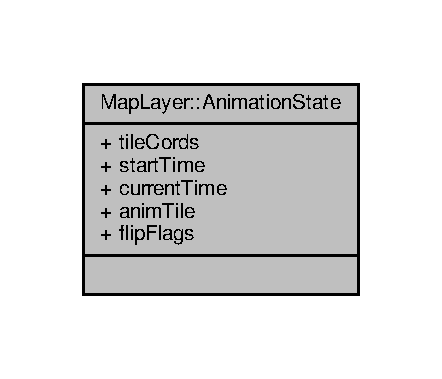
\includegraphics[width=212pt]{structMapLayer_1_1AnimationState__coll__graph}
\end{center}
\end{figure}
\subsection*{Public Attributes}
\begin{DoxyCompactItemize}
\item 
sf\+::\+Vector2u \hyperlink{structMapLayer_1_1AnimationState_ab37c9495a8dce1f661f1f4e46b77f17f}{tile\+Cords}
\item 
sf\+::\+Time \hyperlink{structMapLayer_1_1AnimationState_aa9d9ceefb1f56dac58bc7660a1ba7898}{start\+Time}
\item 
sf\+::\+Time \hyperlink{structMapLayer_1_1AnimationState_a836c7a2799636527b08eeeb1783069e8}{current\+Time}
\item 
tmx\+::\+Tileset\+::\+Tile \hyperlink{structMapLayer_1_1AnimationState_aabe80ae4711c86db562b3e7b5e3bb6d1}{anim\+Tile}
\item 
std\+::uint8\+\_\+t \hyperlink{structMapLayer_1_1AnimationState_aa880baa2bb7e1e2f02d37ce7a6c0dc8a}{flip\+Flags}
\end{DoxyCompactItemize}


\subsection{Member Data Documentation}
\mbox{\Hypertarget{structMapLayer_1_1AnimationState_aabe80ae4711c86db562b3e7b5e3bb6d1}\label{structMapLayer_1_1AnimationState_aabe80ae4711c86db562b3e7b5e3bb6d1}} 
\index{Map\+Layer\+::\+Animation\+State@{Map\+Layer\+::\+Animation\+State}!anim\+Tile@{anim\+Tile}}
\index{anim\+Tile@{anim\+Tile}!Map\+Layer\+::\+Animation\+State@{Map\+Layer\+::\+Animation\+State}}
\subsubsection{\texorpdfstring{anim\+Tile}{animTile}}
{\footnotesize\ttfamily tmx\+::\+Tileset\+::\+Tile Map\+Layer\+::\+Animation\+State\+::anim\+Tile}

\mbox{\Hypertarget{structMapLayer_1_1AnimationState_a836c7a2799636527b08eeeb1783069e8}\label{structMapLayer_1_1AnimationState_a836c7a2799636527b08eeeb1783069e8}} 
\index{Map\+Layer\+::\+Animation\+State@{Map\+Layer\+::\+Animation\+State}!current\+Time@{current\+Time}}
\index{current\+Time@{current\+Time}!Map\+Layer\+::\+Animation\+State@{Map\+Layer\+::\+Animation\+State}}
\subsubsection{\texorpdfstring{current\+Time}{currentTime}}
{\footnotesize\ttfamily sf\+::\+Time Map\+Layer\+::\+Animation\+State\+::current\+Time}

\mbox{\Hypertarget{structMapLayer_1_1AnimationState_aa880baa2bb7e1e2f02d37ce7a6c0dc8a}\label{structMapLayer_1_1AnimationState_aa880baa2bb7e1e2f02d37ce7a6c0dc8a}} 
\index{Map\+Layer\+::\+Animation\+State@{Map\+Layer\+::\+Animation\+State}!flip\+Flags@{flip\+Flags}}
\index{flip\+Flags@{flip\+Flags}!Map\+Layer\+::\+Animation\+State@{Map\+Layer\+::\+Animation\+State}}
\subsubsection{\texorpdfstring{flip\+Flags}{flipFlags}}
{\footnotesize\ttfamily std\+::uint8\+\_\+t Map\+Layer\+::\+Animation\+State\+::flip\+Flags}

\mbox{\Hypertarget{structMapLayer_1_1AnimationState_aa9d9ceefb1f56dac58bc7660a1ba7898}\label{structMapLayer_1_1AnimationState_aa9d9ceefb1f56dac58bc7660a1ba7898}} 
\index{Map\+Layer\+::\+Animation\+State@{Map\+Layer\+::\+Animation\+State}!start\+Time@{start\+Time}}
\index{start\+Time@{start\+Time}!Map\+Layer\+::\+Animation\+State@{Map\+Layer\+::\+Animation\+State}}
\subsubsection{\texorpdfstring{start\+Time}{startTime}}
{\footnotesize\ttfamily sf\+::\+Time Map\+Layer\+::\+Animation\+State\+::start\+Time}

\mbox{\Hypertarget{structMapLayer_1_1AnimationState_ab37c9495a8dce1f661f1f4e46b77f17f}\label{structMapLayer_1_1AnimationState_ab37c9495a8dce1f661f1f4e46b77f17f}} 
\index{Map\+Layer\+::\+Animation\+State@{Map\+Layer\+::\+Animation\+State}!tile\+Cords@{tile\+Cords}}
\index{tile\+Cords@{tile\+Cords}!Map\+Layer\+::\+Animation\+State@{Map\+Layer\+::\+Animation\+State}}
\subsubsection{\texorpdfstring{tile\+Cords}{tileCords}}
{\footnotesize\ttfamily sf\+::\+Vector2u Map\+Layer\+::\+Animation\+State\+::tile\+Cords}



The documentation for this struct was generated from the following file\+:\begin{DoxyCompactItemize}
\item 
/mnt/hdd/\+C0de/\+Engines/\+S\+F\+M\+L/\+S\+F\+M\+L\+\_\+\+Engine/include/\hyperlink{SFMLOrthogonalLayer_8hpp}{S\+F\+M\+L\+Orthogonal\+Layer.\+hpp}\end{DoxyCompactItemize}

\hypertarget{structb0x__2d__SHAPES}{}\section{b0x\+\_\+2d\+\_\+\+S\+H\+A\+P\+ES Struct Reference}
\label{structb0x__2d__SHAPES}\index{b0x\+\_\+2d\+\_\+\+S\+H\+A\+P\+ES@{b0x\+\_\+2d\+\_\+\+S\+H\+A\+P\+ES}}


{\ttfamily \#include $<$entity.\+h$>$}



Collaboration diagram for b0x\+\_\+2d\+\_\+\+S\+H\+A\+P\+ES\+:
\nopagebreak
\begin{figure}[H]
\begin{center}
\leavevmode
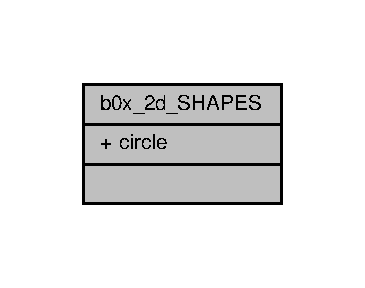
\includegraphics[width=175pt]{structb0x__2d__SHAPES__coll__graph}
\end{center}
\end{figure}
\subsection*{Public Attributes}
\begin{DoxyCompactItemize}
\item 
b2\+Circle\+Shape \hyperlink{structb0x__2d__SHAPES_ac328aa711add03e4823470a27d286122}{circle}
\end{DoxyCompactItemize}


\subsection{Member Data Documentation}
\mbox{\Hypertarget{structb0x__2d__SHAPES_ac328aa711add03e4823470a27d286122}\label{structb0x__2d__SHAPES_ac328aa711add03e4823470a27d286122}} 
\index{b0x\+\_\+2d\+\_\+\+S\+H\+A\+P\+ES@{b0x\+\_\+2d\+\_\+\+S\+H\+A\+P\+ES}!circle@{circle}}
\index{circle@{circle}!b0x\+\_\+2d\+\_\+\+S\+H\+A\+P\+ES@{b0x\+\_\+2d\+\_\+\+S\+H\+A\+P\+ES}}
\subsubsection{\texorpdfstring{circle}{circle}}
{\footnotesize\ttfamily b2\+Circle\+Shape b0x\+\_\+2d\+\_\+\+S\+H\+A\+P\+E\+S\+::circle}



The documentation for this struct was generated from the following file\+:\begin{DoxyCompactItemize}
\item 
/mnt/hdd/\+C0de/smart\+\_\+engine/include/\hyperlink{entity_8h}{entity.\+h}\end{DoxyCompactItemize}

\hypertarget{structCharacter}{}\section{Character Struct Reference}
\label{structCharacter}\index{Character@{Character}}


Holds all state information relevant to a character as loaded using Free\+Type.  




{\ttfamily \#include $<$text\+\_\+renderer.\+h$>$}



Collaboration diagram for Character\+:
\nopagebreak
\begin{figure}[H]
\begin{center}
\leavevmode
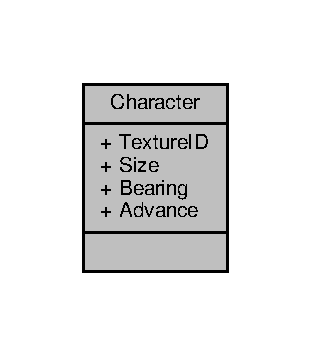
\includegraphics[width=149pt]{structCharacter__coll__graph}
\end{center}
\end{figure}
\subsection*{Public Attributes}
\begin{DoxyCompactItemize}
\item 
unsigned int \hyperlink{structCharacter_a411760a6a33f2cb54dd6a0138e038a46}{Texture\+ID}
\item 
glm\+::ivec2 \hyperlink{structCharacter_aaaa598050e0ef590fe6903fd2bab40b8}{Size}
\item 
glm\+::ivec2 \hyperlink{structCharacter_afef98bf9c7f5313d96476f6f3f85f872}{Bearing}
\item 
unsigned int \hyperlink{structCharacter_a5338c0800545802a63f8e4945573cbe7}{Advance}
\end{DoxyCompactItemize}


\subsection{Detailed Description}
Holds all state information relevant to a character as loaded using Free\+Type. 

\subsection{Member Data Documentation}
\mbox{\Hypertarget{structCharacter_a5338c0800545802a63f8e4945573cbe7}\label{structCharacter_a5338c0800545802a63f8e4945573cbe7}} 
\index{Character@{Character}!Advance@{Advance}}
\index{Advance@{Advance}!Character@{Character}}
\subsubsection{\texorpdfstring{Advance}{Advance}}
{\footnotesize\ttfamily unsigned int Character\+::\+Advance}

\mbox{\Hypertarget{structCharacter_afef98bf9c7f5313d96476f6f3f85f872}\label{structCharacter_afef98bf9c7f5313d96476f6f3f85f872}} 
\index{Character@{Character}!Bearing@{Bearing}}
\index{Bearing@{Bearing}!Character@{Character}}
\subsubsection{\texorpdfstring{Bearing}{Bearing}}
{\footnotesize\ttfamily glm\+::ivec2 Character\+::\+Bearing}

\mbox{\Hypertarget{structCharacter_aaaa598050e0ef590fe6903fd2bab40b8}\label{structCharacter_aaaa598050e0ef590fe6903fd2bab40b8}} 
\index{Character@{Character}!Size@{Size}}
\index{Size@{Size}!Character@{Character}}
\subsubsection{\texorpdfstring{Size}{Size}}
{\footnotesize\ttfamily glm\+::ivec2 Character\+::\+Size}

\mbox{\Hypertarget{structCharacter_a411760a6a33f2cb54dd6a0138e038a46}\label{structCharacter_a411760a6a33f2cb54dd6a0138e038a46}} 
\index{Character@{Character}!Texture\+ID@{Texture\+ID}}
\index{Texture\+ID@{Texture\+ID}!Character@{Character}}
\subsubsection{\texorpdfstring{Texture\+ID}{TextureID}}
{\footnotesize\ttfamily unsigned int Character\+::\+Texture\+ID}



The documentation for this struct was generated from the following file\+:\begin{DoxyCompactItemize}
\item 
/mnt/hdd/\+C0de/smart\+\_\+engine/include/\hyperlink{text__renderer_8h}{text\+\_\+renderer.\+h}\end{DoxyCompactItemize}

\hypertarget{classMapLayer_1_1Chunk}{}\section{Map\+Layer\+:\+:Chunk Class Reference}
\label{classMapLayer_1_1Chunk}\index{Map\+Layer\+::\+Chunk@{Map\+Layer\+::\+Chunk}}


Inheritance diagram for Map\+Layer\+:\+:Chunk\+:
\nopagebreak
\begin{figure}[H]
\begin{center}
\leavevmode
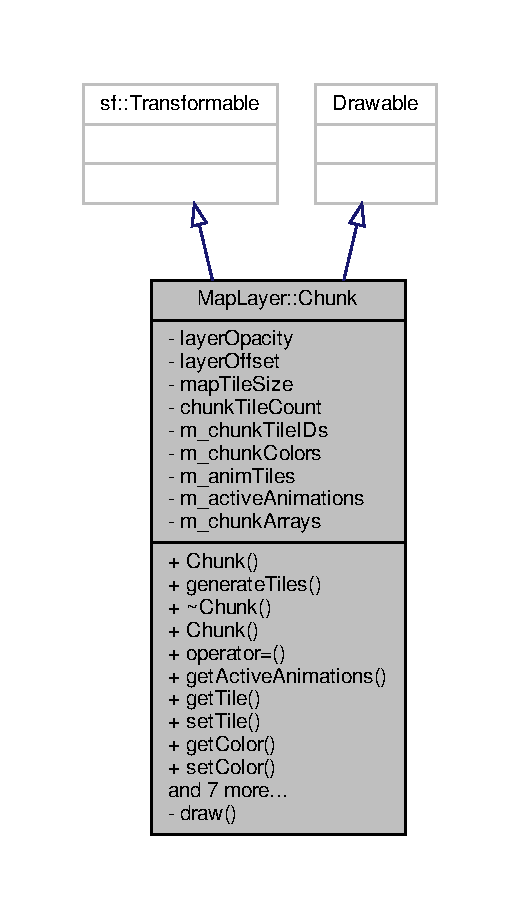
\includegraphics[width=235pt]{classMapLayer_1_1Chunk__inherit__graph}
\end{center}
\end{figure}


Collaboration diagram for Map\+Layer\+:\+:Chunk\+:
\nopagebreak
\begin{figure}[H]
\begin{center}
\leavevmode
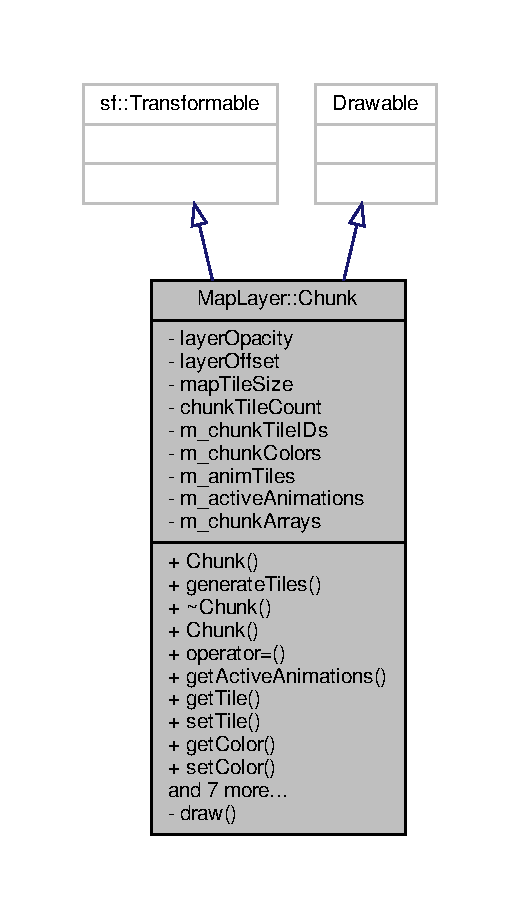
\includegraphics[width=235pt]{classMapLayer_1_1Chunk__coll__graph}
\end{center}
\end{figure}
\subsection*{Classes}
\begin{DoxyCompactItemize}
\item 
class \hyperlink{classMapLayer_1_1Chunk_1_1ChunkArray}{Chunk\+Array}
\end{DoxyCompactItemize}
\subsection*{Public Types}
\begin{DoxyCompactItemize}
\item 
using \hyperlink{classMapLayer_1_1Chunk_ab1df4d3621c5d9f83c2edb46d0744078}{Ptr} = std\+::unique\+\_\+ptr$<$ \hyperlink{classMapLayer_1_1Chunk}{Chunk} $>$
\item 
using \hyperlink{classMapLayer_1_1Chunk_a2137a288bfd4120eb3e4db5934b802f3}{Tile} = std\+::array$<$ sf\+::\+Vertex, 4u $>$
\end{DoxyCompactItemize}
\subsection*{Public Member Functions}
\begin{DoxyCompactItemize}
\item 
\hyperlink{classMapLayer_1_1Chunk_a793a265040a7e0e117d47463b5d1f762}{Chunk} (const tmx\+::\+Tile\+Layer \&layer, std\+::vector$<$ const tmx\+::\+Tileset $\ast$$>$ tilesets, const sf\+::\+Vector2f \&position, const sf\+::\+Vector2f \&tile\+Count, const sf\+::\+Vector2u \&tile\+Size, std\+::size\+\_\+t row\+Size, \hyperlink{classMapLayer_a64011087426e436e3cb8374570378d68}{Texture\+Resource} \&tr, const std\+::map$<$ std\+::uint32\+\_\+t, tmx\+::\+Tileset\+::\+Tile $>$ \&anim\+Tiles)
\item 
void \hyperlink{classMapLayer_1_1Chunk_aa8e16ad1e2e77a00313c4ed92f0a87b7}{generate\+Tiles} (bool register\+Animation=false)
\item 
\hyperlink{classMapLayer_1_1Chunk_a868f8750a2139ead6a79ae6f228303f5}{$\sim$\+Chunk} ()=default
\item 
\hyperlink{classMapLayer_1_1Chunk_ad135fca4082657b3babebd9c5b3402a8}{Chunk} (const \hyperlink{classMapLayer_1_1Chunk}{Chunk} \&)=delete
\item 
\hyperlink{classMapLayer_1_1Chunk}{Chunk} \& \hyperlink{classMapLayer_1_1Chunk_aad57eee35df69297877377ac64dceb6f}{operator=} (const \hyperlink{classMapLayer_1_1Chunk}{Chunk} \&)=delete
\item 
std\+::vector$<$ \hyperlink{structMapLayer_1_1AnimationState}{Animation\+State} $>$ \& \hyperlink{classMapLayer_1_1Chunk_adc0fdad3f30d7ff327b2a538efc8c949}{get\+Active\+Animations} ()
\item 
tmx\+::\+Tile\+Layer\+::\+Tile \hyperlink{classMapLayer_1_1Chunk_ae70972baf5ed18a69709f180e62f4eb5}{get\+Tile} (int x, int y) const
\item 
void \hyperlink{classMapLayer_1_1Chunk_a557343f1e955e78b6f68623007fb9a7a}{set\+Tile} (int x, int y, tmx\+::\+Tile\+Layer\+::\+Tile tile, bool refresh)
\item 
sf\+::\+Color \hyperlink{classMapLayer_1_1Chunk_aeee5ad34f7c428e1fd290b2a1a695397}{get\+Color} (int x, int y) const
\item 
void \hyperlink{classMapLayer_1_1Chunk_addf26b112e46bc6995f03a886cf46dc8}{set\+Color} (int x, int y, sf\+::\+Color color, bool refresh)
\item 
void \hyperlink{classMapLayer_1_1Chunk_abf755ab4f7b9430aae29a631eb2ee48e}{maybe\+Regenerate} (bool refresh)
\item 
int \hyperlink{classMapLayer_1_1Chunk_a3df37cf62d435f242780c6ae3cf0f339}{calc\+Index\+From} (int x, int y) const
\item 
bool \hyperlink{classMapLayer_1_1Chunk_ad7e91d957e932e8c4235f5008cbd03c8}{empty} () const
\item 
void \hyperlink{classMapLayer_1_1Chunk_a6de781e426b23c3b33e34a1ea70eb14f}{flipY} (sf\+::\+Vector2f $\ast$v0, sf\+::\+Vector2f $\ast$v1, sf\+::\+Vector2f $\ast$v2, sf\+::\+Vector2f $\ast$v3)
\item 
void \hyperlink{classMapLayer_1_1Chunk_a0bd785f9c54b97ae99417261210b9579}{flipX} (sf\+::\+Vector2f $\ast$v0, sf\+::\+Vector2f $\ast$v1, sf\+::\+Vector2f $\ast$v2, sf\+::\+Vector2f $\ast$v3)
\item 
void \hyperlink{classMapLayer_1_1Chunk_a82346cb03113d15eb2b135c082257b0e}{flipD} (sf\+::\+Vector2f $\ast$v0, sf\+::\+Vector2f $\ast$v1, sf\+::\+Vector2f $\ast$v2, sf\+::\+Vector2f $\ast$v3)
\item 
void \hyperlink{classMapLayer_1_1Chunk_ac90c3c9041c12cf6955707966c20d0cc}{do\+Flips} (std\+::uint8\+\_\+t bits, sf\+::\+Vector2f $\ast$v0, sf\+::\+Vector2f $\ast$v1, sf\+::\+Vector2f $\ast$v2, sf\+::\+Vector2f $\ast$v3)
\end{DoxyCompactItemize}
\subsection*{Private Member Functions}
\begin{DoxyCompactItemize}
\item 
void \hyperlink{classMapLayer_1_1Chunk_ab2f932fad581f2dd23d1570ebb4c76b9}{draw} (sf\+::\+Render\+Target \&rt, sf\+::\+Render\+States states) const override
\end{DoxyCompactItemize}
\subsection*{Private Attributes}
\begin{DoxyCompactItemize}
\item 
sf\+::\+Uint8 \hyperlink{classMapLayer_1_1Chunk_a2540be672f38d7f6826eebb944881429}{layer\+Opacity}
\item 
sf\+::\+Vector2f \hyperlink{classMapLayer_1_1Chunk_a58aafb7ea1d939755673bef91bfe313e}{layer\+Offset}
\item 
sf\+::\+Vector2u \hyperlink{classMapLayer_1_1Chunk_a010215bc42e515278da75b680c88dcdf}{map\+Tile\+Size}
\item 
sf\+::\+Vector2f \hyperlink{classMapLayer_1_1Chunk_a48d8fc51f7358f229818659ae7869485}{chunk\+Tile\+Count}
\item 
std\+::vector$<$ tmx\+::\+Tile\+Layer\+::\+Tile $>$ \hyperlink{classMapLayer_1_1Chunk_ab40e4c80d3c205fc62db6a1c90e6afe7}{m\+\_\+chunk\+Tile\+I\+Ds}
\item 
std\+::vector$<$ sf\+::\+Color $>$ \hyperlink{classMapLayer_1_1Chunk_ab09b61a5d77f4acad152ac60db3cd333}{m\+\_\+chunk\+Colors}
\item 
std\+::map$<$ std\+::uint32\+\_\+t, tmx\+::\+Tileset\+::\+Tile $>$ \hyperlink{classMapLayer_1_1Chunk_a70854589957a8232358b04f971c1a1ec}{m\+\_\+anim\+Tiles}
\item 
std\+::vector$<$ \hyperlink{structMapLayer_1_1AnimationState}{Animation\+State} $>$ \hyperlink{classMapLayer_1_1Chunk_a8b618ddd7286a02a668fb9f8404427b6}{m\+\_\+active\+Animations}
\item 
std\+::vector$<$ \hyperlink{classMapLayer_1_1Chunk_1_1ChunkArray_a6d944dee2fc89a76d7a252405e2732b0}{Chunk\+Array\+::\+Ptr} $>$ \hyperlink{classMapLayer_1_1Chunk_ab264049d7a576a9b8efd88df159704bf}{m\+\_\+chunk\+Arrays}
\end{DoxyCompactItemize}


\subsection{Member Typedef Documentation}
\mbox{\Hypertarget{classMapLayer_1_1Chunk_ab1df4d3621c5d9f83c2edb46d0744078}\label{classMapLayer_1_1Chunk_ab1df4d3621c5d9f83c2edb46d0744078}} 
\index{Map\+Layer\+::\+Chunk@{Map\+Layer\+::\+Chunk}!Ptr@{Ptr}}
\index{Ptr@{Ptr}!Map\+Layer\+::\+Chunk@{Map\+Layer\+::\+Chunk}}
\subsubsection{\texorpdfstring{Ptr}{Ptr}}
{\footnotesize\ttfamily using \hyperlink{classMapLayer_1_1Chunk_ab1df4d3621c5d9f83c2edb46d0744078}{Map\+Layer\+::\+Chunk\+::\+Ptr} =  std\+::unique\+\_\+ptr$<$\hyperlink{classMapLayer_1_1Chunk}{Chunk}$>$}

\mbox{\Hypertarget{classMapLayer_1_1Chunk_a2137a288bfd4120eb3e4db5934b802f3}\label{classMapLayer_1_1Chunk_a2137a288bfd4120eb3e4db5934b802f3}} 
\index{Map\+Layer\+::\+Chunk@{Map\+Layer\+::\+Chunk}!Tile@{Tile}}
\index{Tile@{Tile}!Map\+Layer\+::\+Chunk@{Map\+Layer\+::\+Chunk}}
\subsubsection{\texorpdfstring{Tile}{Tile}}
{\footnotesize\ttfamily using \hyperlink{classMapLayer_1_1Chunk_a2137a288bfd4120eb3e4db5934b802f3}{Map\+Layer\+::\+Chunk\+::\+Tile} =  std\+::array$<$sf\+::\+Vertex, 4u$>$}



\subsection{Constructor \& Destructor Documentation}
\mbox{\Hypertarget{classMapLayer_1_1Chunk_a793a265040a7e0e117d47463b5d1f762}\label{classMapLayer_1_1Chunk_a793a265040a7e0e117d47463b5d1f762}} 
\index{Map\+Layer\+::\+Chunk@{Map\+Layer\+::\+Chunk}!Chunk@{Chunk}}
\index{Chunk@{Chunk}!Map\+Layer\+::\+Chunk@{Map\+Layer\+::\+Chunk}}
\subsubsection{\texorpdfstring{Chunk()}{Chunk()}\hspace{0.1cm}{\footnotesize\ttfamily [1/2]}}
{\footnotesize\ttfamily Map\+Layer\+::\+Chunk\+::\+Chunk (\begin{DoxyParamCaption}\item[{const tmx\+::\+Tile\+Layer \&}]{layer,  }\item[{std\+::vector$<$ const tmx\+::\+Tileset $\ast$$>$}]{tilesets,  }\item[{const sf\+::\+Vector2f \&}]{position,  }\item[{const sf\+::\+Vector2f \&}]{tile\+Count,  }\item[{const sf\+::\+Vector2u \&}]{tile\+Size,  }\item[{std\+::size\+\_\+t}]{row\+Size,  }\item[{\hyperlink{classMapLayer_a64011087426e436e3cb8374570378d68}{Texture\+Resource} \&}]{tr,  }\item[{const std\+::map$<$ std\+::uint32\+\_\+t, tmx\+::\+Tileset\+::\+Tile $>$ \&}]{anim\+Tiles }\end{DoxyParamCaption})\hspace{0.3cm}{\ttfamily [inline]}}

\mbox{\Hypertarget{classMapLayer_1_1Chunk_a868f8750a2139ead6a79ae6f228303f5}\label{classMapLayer_1_1Chunk_a868f8750a2139ead6a79ae6f228303f5}} 
\index{Map\+Layer\+::\+Chunk@{Map\+Layer\+::\+Chunk}!````~Chunk@{$\sim$\+Chunk}}
\index{````~Chunk@{$\sim$\+Chunk}!Map\+Layer\+::\+Chunk@{Map\+Layer\+::\+Chunk}}
\subsubsection{\texorpdfstring{$\sim$\+Chunk()}{~Chunk()}}
{\footnotesize\ttfamily Map\+Layer\+::\+Chunk\+::$\sim$\+Chunk (\begin{DoxyParamCaption}{ }\end{DoxyParamCaption})\hspace{0.3cm}{\ttfamily [default]}}

\mbox{\Hypertarget{classMapLayer_1_1Chunk_ad135fca4082657b3babebd9c5b3402a8}\label{classMapLayer_1_1Chunk_ad135fca4082657b3babebd9c5b3402a8}} 
\index{Map\+Layer\+::\+Chunk@{Map\+Layer\+::\+Chunk}!Chunk@{Chunk}}
\index{Chunk@{Chunk}!Map\+Layer\+::\+Chunk@{Map\+Layer\+::\+Chunk}}
\subsubsection{\texorpdfstring{Chunk()}{Chunk()}\hspace{0.1cm}{\footnotesize\ttfamily [2/2]}}
{\footnotesize\ttfamily Map\+Layer\+::\+Chunk\+::\+Chunk (\begin{DoxyParamCaption}\item[{const \hyperlink{classMapLayer_1_1Chunk}{Chunk} \&}]{ }\end{DoxyParamCaption})\hspace{0.3cm}{\ttfamily [delete]}}



\subsection{Member Function Documentation}
\mbox{\Hypertarget{classMapLayer_1_1Chunk_a3df37cf62d435f242780c6ae3cf0f339}\label{classMapLayer_1_1Chunk_a3df37cf62d435f242780c6ae3cf0f339}} 
\index{Map\+Layer\+::\+Chunk@{Map\+Layer\+::\+Chunk}!calc\+Index\+From@{calc\+Index\+From}}
\index{calc\+Index\+From@{calc\+Index\+From}!Map\+Layer\+::\+Chunk@{Map\+Layer\+::\+Chunk}}
\subsubsection{\texorpdfstring{calc\+Index\+From()}{calcIndexFrom()}}
{\footnotesize\ttfamily int Map\+Layer\+::\+Chunk\+::calc\+Index\+From (\begin{DoxyParamCaption}\item[{int}]{x,  }\item[{int}]{y }\end{DoxyParamCaption}) const\hspace{0.3cm}{\ttfamily [inline]}}

\mbox{\Hypertarget{classMapLayer_1_1Chunk_ac90c3c9041c12cf6955707966c20d0cc}\label{classMapLayer_1_1Chunk_ac90c3c9041c12cf6955707966c20d0cc}} 
\index{Map\+Layer\+::\+Chunk@{Map\+Layer\+::\+Chunk}!do\+Flips@{do\+Flips}}
\index{do\+Flips@{do\+Flips}!Map\+Layer\+::\+Chunk@{Map\+Layer\+::\+Chunk}}
\subsubsection{\texorpdfstring{do\+Flips()}{doFlips()}}
{\footnotesize\ttfamily void Map\+Layer\+::\+Chunk\+::do\+Flips (\begin{DoxyParamCaption}\item[{std\+::uint8\+\_\+t}]{bits,  }\item[{sf\+::\+Vector2f $\ast$}]{v0,  }\item[{sf\+::\+Vector2f $\ast$}]{v1,  }\item[{sf\+::\+Vector2f $\ast$}]{v2,  }\item[{sf\+::\+Vector2f $\ast$}]{v3 }\end{DoxyParamCaption})\hspace{0.3cm}{\ttfamily [inline]}}

\mbox{\Hypertarget{classMapLayer_1_1Chunk_ab2f932fad581f2dd23d1570ebb4c76b9}\label{classMapLayer_1_1Chunk_ab2f932fad581f2dd23d1570ebb4c76b9}} 
\index{Map\+Layer\+::\+Chunk@{Map\+Layer\+::\+Chunk}!draw@{draw}}
\index{draw@{draw}!Map\+Layer\+::\+Chunk@{Map\+Layer\+::\+Chunk}}
\subsubsection{\texorpdfstring{draw()}{draw()}}
{\footnotesize\ttfamily void Map\+Layer\+::\+Chunk\+::draw (\begin{DoxyParamCaption}\item[{sf\+::\+Render\+Target \&}]{rt,  }\item[{sf\+::\+Render\+States}]{states }\end{DoxyParamCaption}) const\hspace{0.3cm}{\ttfamily [inline]}, {\ttfamily [override]}, {\ttfamily [private]}}

\mbox{\Hypertarget{classMapLayer_1_1Chunk_ad7e91d957e932e8c4235f5008cbd03c8}\label{classMapLayer_1_1Chunk_ad7e91d957e932e8c4235f5008cbd03c8}} 
\index{Map\+Layer\+::\+Chunk@{Map\+Layer\+::\+Chunk}!empty@{empty}}
\index{empty@{empty}!Map\+Layer\+::\+Chunk@{Map\+Layer\+::\+Chunk}}
\subsubsection{\texorpdfstring{empty()}{empty()}}
{\footnotesize\ttfamily bool Map\+Layer\+::\+Chunk\+::empty (\begin{DoxyParamCaption}{ }\end{DoxyParamCaption}) const\hspace{0.3cm}{\ttfamily [inline]}}

\mbox{\Hypertarget{classMapLayer_1_1Chunk_a82346cb03113d15eb2b135c082257b0e}\label{classMapLayer_1_1Chunk_a82346cb03113d15eb2b135c082257b0e}} 
\index{Map\+Layer\+::\+Chunk@{Map\+Layer\+::\+Chunk}!flipD@{flipD}}
\index{flipD@{flipD}!Map\+Layer\+::\+Chunk@{Map\+Layer\+::\+Chunk}}
\subsubsection{\texorpdfstring{flip\+D()}{flipD()}}
{\footnotesize\ttfamily void Map\+Layer\+::\+Chunk\+::flipD (\begin{DoxyParamCaption}\item[{sf\+::\+Vector2f $\ast$}]{v0,  }\item[{sf\+::\+Vector2f $\ast$}]{v1,  }\item[{sf\+::\+Vector2f $\ast$}]{v2,  }\item[{sf\+::\+Vector2f $\ast$}]{v3 }\end{DoxyParamCaption})\hspace{0.3cm}{\ttfamily [inline]}}

\mbox{\Hypertarget{classMapLayer_1_1Chunk_a0bd785f9c54b97ae99417261210b9579}\label{classMapLayer_1_1Chunk_a0bd785f9c54b97ae99417261210b9579}} 
\index{Map\+Layer\+::\+Chunk@{Map\+Layer\+::\+Chunk}!flipX@{flipX}}
\index{flipX@{flipX}!Map\+Layer\+::\+Chunk@{Map\+Layer\+::\+Chunk}}
\subsubsection{\texorpdfstring{flip\+X()}{flipX()}}
{\footnotesize\ttfamily void Map\+Layer\+::\+Chunk\+::flipX (\begin{DoxyParamCaption}\item[{sf\+::\+Vector2f $\ast$}]{v0,  }\item[{sf\+::\+Vector2f $\ast$}]{v1,  }\item[{sf\+::\+Vector2f $\ast$}]{v2,  }\item[{sf\+::\+Vector2f $\ast$}]{v3 }\end{DoxyParamCaption})\hspace{0.3cm}{\ttfamily [inline]}}

\mbox{\Hypertarget{classMapLayer_1_1Chunk_a6de781e426b23c3b33e34a1ea70eb14f}\label{classMapLayer_1_1Chunk_a6de781e426b23c3b33e34a1ea70eb14f}} 
\index{Map\+Layer\+::\+Chunk@{Map\+Layer\+::\+Chunk}!flipY@{flipY}}
\index{flipY@{flipY}!Map\+Layer\+::\+Chunk@{Map\+Layer\+::\+Chunk}}
\subsubsection{\texorpdfstring{flip\+Y()}{flipY()}}
{\footnotesize\ttfamily void Map\+Layer\+::\+Chunk\+::flipY (\begin{DoxyParamCaption}\item[{sf\+::\+Vector2f $\ast$}]{v0,  }\item[{sf\+::\+Vector2f $\ast$}]{v1,  }\item[{sf\+::\+Vector2f $\ast$}]{v2,  }\item[{sf\+::\+Vector2f $\ast$}]{v3 }\end{DoxyParamCaption})\hspace{0.3cm}{\ttfamily [inline]}}

\mbox{\Hypertarget{classMapLayer_1_1Chunk_aa8e16ad1e2e77a00313c4ed92f0a87b7}\label{classMapLayer_1_1Chunk_aa8e16ad1e2e77a00313c4ed92f0a87b7}} 
\index{Map\+Layer\+::\+Chunk@{Map\+Layer\+::\+Chunk}!generate\+Tiles@{generate\+Tiles}}
\index{generate\+Tiles@{generate\+Tiles}!Map\+Layer\+::\+Chunk@{Map\+Layer\+::\+Chunk}}
\subsubsection{\texorpdfstring{generate\+Tiles()}{generateTiles()}}
{\footnotesize\ttfamily void Map\+Layer\+::\+Chunk\+::generate\+Tiles (\begin{DoxyParamCaption}\item[{bool}]{register\+Animation = {\ttfamily false} }\end{DoxyParamCaption})\hspace{0.3cm}{\ttfamily [inline]}}

\mbox{\Hypertarget{classMapLayer_1_1Chunk_adc0fdad3f30d7ff327b2a538efc8c949}\label{classMapLayer_1_1Chunk_adc0fdad3f30d7ff327b2a538efc8c949}} 
\index{Map\+Layer\+::\+Chunk@{Map\+Layer\+::\+Chunk}!get\+Active\+Animations@{get\+Active\+Animations}}
\index{get\+Active\+Animations@{get\+Active\+Animations}!Map\+Layer\+::\+Chunk@{Map\+Layer\+::\+Chunk}}
\subsubsection{\texorpdfstring{get\+Active\+Animations()}{getActiveAnimations()}}
{\footnotesize\ttfamily std\+::vector$<$\hyperlink{structMapLayer_1_1AnimationState}{Animation\+State}$>$\& Map\+Layer\+::\+Chunk\+::get\+Active\+Animations (\begin{DoxyParamCaption}{ }\end{DoxyParamCaption})\hspace{0.3cm}{\ttfamily [inline]}}

\mbox{\Hypertarget{classMapLayer_1_1Chunk_aeee5ad34f7c428e1fd290b2a1a695397}\label{classMapLayer_1_1Chunk_aeee5ad34f7c428e1fd290b2a1a695397}} 
\index{Map\+Layer\+::\+Chunk@{Map\+Layer\+::\+Chunk}!get\+Color@{get\+Color}}
\index{get\+Color@{get\+Color}!Map\+Layer\+::\+Chunk@{Map\+Layer\+::\+Chunk}}
\subsubsection{\texorpdfstring{get\+Color()}{getColor()}}
{\footnotesize\ttfamily sf\+::\+Color Map\+Layer\+::\+Chunk\+::get\+Color (\begin{DoxyParamCaption}\item[{int}]{x,  }\item[{int}]{y }\end{DoxyParamCaption}) const\hspace{0.3cm}{\ttfamily [inline]}}

\mbox{\Hypertarget{classMapLayer_1_1Chunk_ae70972baf5ed18a69709f180e62f4eb5}\label{classMapLayer_1_1Chunk_ae70972baf5ed18a69709f180e62f4eb5}} 
\index{Map\+Layer\+::\+Chunk@{Map\+Layer\+::\+Chunk}!get\+Tile@{get\+Tile}}
\index{get\+Tile@{get\+Tile}!Map\+Layer\+::\+Chunk@{Map\+Layer\+::\+Chunk}}
\subsubsection{\texorpdfstring{get\+Tile()}{getTile()}}
{\footnotesize\ttfamily tmx\+::\+Tile\+Layer\+::\+Tile Map\+Layer\+::\+Chunk\+::get\+Tile (\begin{DoxyParamCaption}\item[{int}]{x,  }\item[{int}]{y }\end{DoxyParamCaption}) const\hspace{0.3cm}{\ttfamily [inline]}}

\mbox{\Hypertarget{classMapLayer_1_1Chunk_abf755ab4f7b9430aae29a631eb2ee48e}\label{classMapLayer_1_1Chunk_abf755ab4f7b9430aae29a631eb2ee48e}} 
\index{Map\+Layer\+::\+Chunk@{Map\+Layer\+::\+Chunk}!maybe\+Regenerate@{maybe\+Regenerate}}
\index{maybe\+Regenerate@{maybe\+Regenerate}!Map\+Layer\+::\+Chunk@{Map\+Layer\+::\+Chunk}}
\subsubsection{\texorpdfstring{maybe\+Regenerate()}{maybeRegenerate()}}
{\footnotesize\ttfamily void Map\+Layer\+::\+Chunk\+::maybe\+Regenerate (\begin{DoxyParamCaption}\item[{bool}]{refresh }\end{DoxyParamCaption})\hspace{0.3cm}{\ttfamily [inline]}}

\mbox{\Hypertarget{classMapLayer_1_1Chunk_aad57eee35df69297877377ac64dceb6f}\label{classMapLayer_1_1Chunk_aad57eee35df69297877377ac64dceb6f}} 
\index{Map\+Layer\+::\+Chunk@{Map\+Layer\+::\+Chunk}!operator=@{operator=}}
\index{operator=@{operator=}!Map\+Layer\+::\+Chunk@{Map\+Layer\+::\+Chunk}}
\subsubsection{\texorpdfstring{operator=()}{operator=()}}
{\footnotesize\ttfamily \hyperlink{classMapLayer_1_1Chunk}{Chunk}\& Map\+Layer\+::\+Chunk\+::operator= (\begin{DoxyParamCaption}\item[{const \hyperlink{classMapLayer_1_1Chunk}{Chunk} \&}]{ }\end{DoxyParamCaption})\hspace{0.3cm}{\ttfamily [delete]}}

\mbox{\Hypertarget{classMapLayer_1_1Chunk_addf26b112e46bc6995f03a886cf46dc8}\label{classMapLayer_1_1Chunk_addf26b112e46bc6995f03a886cf46dc8}} 
\index{Map\+Layer\+::\+Chunk@{Map\+Layer\+::\+Chunk}!set\+Color@{set\+Color}}
\index{set\+Color@{set\+Color}!Map\+Layer\+::\+Chunk@{Map\+Layer\+::\+Chunk}}
\subsubsection{\texorpdfstring{set\+Color()}{setColor()}}
{\footnotesize\ttfamily void Map\+Layer\+::\+Chunk\+::set\+Color (\begin{DoxyParamCaption}\item[{int}]{x,  }\item[{int}]{y,  }\item[{sf\+::\+Color}]{color,  }\item[{bool}]{refresh }\end{DoxyParamCaption})\hspace{0.3cm}{\ttfamily [inline]}}

\mbox{\Hypertarget{classMapLayer_1_1Chunk_a557343f1e955e78b6f68623007fb9a7a}\label{classMapLayer_1_1Chunk_a557343f1e955e78b6f68623007fb9a7a}} 
\index{Map\+Layer\+::\+Chunk@{Map\+Layer\+::\+Chunk}!set\+Tile@{set\+Tile}}
\index{set\+Tile@{set\+Tile}!Map\+Layer\+::\+Chunk@{Map\+Layer\+::\+Chunk}}
\subsubsection{\texorpdfstring{set\+Tile()}{setTile()}}
{\footnotesize\ttfamily void Map\+Layer\+::\+Chunk\+::set\+Tile (\begin{DoxyParamCaption}\item[{int}]{x,  }\item[{int}]{y,  }\item[{tmx\+::\+Tile\+Layer\+::\+Tile}]{tile,  }\item[{bool}]{refresh }\end{DoxyParamCaption})\hspace{0.3cm}{\ttfamily [inline]}}



\subsection{Member Data Documentation}
\mbox{\Hypertarget{classMapLayer_1_1Chunk_a48d8fc51f7358f229818659ae7869485}\label{classMapLayer_1_1Chunk_a48d8fc51f7358f229818659ae7869485}} 
\index{Map\+Layer\+::\+Chunk@{Map\+Layer\+::\+Chunk}!chunk\+Tile\+Count@{chunk\+Tile\+Count}}
\index{chunk\+Tile\+Count@{chunk\+Tile\+Count}!Map\+Layer\+::\+Chunk@{Map\+Layer\+::\+Chunk}}
\subsubsection{\texorpdfstring{chunk\+Tile\+Count}{chunkTileCount}}
{\footnotesize\ttfamily sf\+::\+Vector2f Map\+Layer\+::\+Chunk\+::chunk\+Tile\+Count\hspace{0.3cm}{\ttfamily [private]}}

\mbox{\Hypertarget{classMapLayer_1_1Chunk_a58aafb7ea1d939755673bef91bfe313e}\label{classMapLayer_1_1Chunk_a58aafb7ea1d939755673bef91bfe313e}} 
\index{Map\+Layer\+::\+Chunk@{Map\+Layer\+::\+Chunk}!layer\+Offset@{layer\+Offset}}
\index{layer\+Offset@{layer\+Offset}!Map\+Layer\+::\+Chunk@{Map\+Layer\+::\+Chunk}}
\subsubsection{\texorpdfstring{layer\+Offset}{layerOffset}}
{\footnotesize\ttfamily sf\+::\+Vector2f Map\+Layer\+::\+Chunk\+::layer\+Offset\hspace{0.3cm}{\ttfamily [private]}}

\mbox{\Hypertarget{classMapLayer_1_1Chunk_a2540be672f38d7f6826eebb944881429}\label{classMapLayer_1_1Chunk_a2540be672f38d7f6826eebb944881429}} 
\index{Map\+Layer\+::\+Chunk@{Map\+Layer\+::\+Chunk}!layer\+Opacity@{layer\+Opacity}}
\index{layer\+Opacity@{layer\+Opacity}!Map\+Layer\+::\+Chunk@{Map\+Layer\+::\+Chunk}}
\subsubsection{\texorpdfstring{layer\+Opacity}{layerOpacity}}
{\footnotesize\ttfamily sf\+::\+Uint8 Map\+Layer\+::\+Chunk\+::layer\+Opacity\hspace{0.3cm}{\ttfamily [private]}}

\mbox{\Hypertarget{classMapLayer_1_1Chunk_a8b618ddd7286a02a668fb9f8404427b6}\label{classMapLayer_1_1Chunk_a8b618ddd7286a02a668fb9f8404427b6}} 
\index{Map\+Layer\+::\+Chunk@{Map\+Layer\+::\+Chunk}!m\+\_\+active\+Animations@{m\+\_\+active\+Animations}}
\index{m\+\_\+active\+Animations@{m\+\_\+active\+Animations}!Map\+Layer\+::\+Chunk@{Map\+Layer\+::\+Chunk}}
\subsubsection{\texorpdfstring{m\+\_\+active\+Animations}{m\_activeAnimations}}
{\footnotesize\ttfamily std\+::vector$<$\hyperlink{structMapLayer_1_1AnimationState}{Animation\+State}$>$ Map\+Layer\+::\+Chunk\+::m\+\_\+active\+Animations\hspace{0.3cm}{\ttfamily [private]}}

\mbox{\Hypertarget{classMapLayer_1_1Chunk_a70854589957a8232358b04f971c1a1ec}\label{classMapLayer_1_1Chunk_a70854589957a8232358b04f971c1a1ec}} 
\index{Map\+Layer\+::\+Chunk@{Map\+Layer\+::\+Chunk}!m\+\_\+anim\+Tiles@{m\+\_\+anim\+Tiles}}
\index{m\+\_\+anim\+Tiles@{m\+\_\+anim\+Tiles}!Map\+Layer\+::\+Chunk@{Map\+Layer\+::\+Chunk}}
\subsubsection{\texorpdfstring{m\+\_\+anim\+Tiles}{m\_animTiles}}
{\footnotesize\ttfamily std\+::map$<$std\+::uint32\+\_\+t, tmx\+::\+Tileset\+::\+Tile$>$ Map\+Layer\+::\+Chunk\+::m\+\_\+anim\+Tiles\hspace{0.3cm}{\ttfamily [private]}}

\mbox{\Hypertarget{classMapLayer_1_1Chunk_ab264049d7a576a9b8efd88df159704bf}\label{classMapLayer_1_1Chunk_ab264049d7a576a9b8efd88df159704bf}} 
\index{Map\+Layer\+::\+Chunk@{Map\+Layer\+::\+Chunk}!m\+\_\+chunk\+Arrays@{m\+\_\+chunk\+Arrays}}
\index{m\+\_\+chunk\+Arrays@{m\+\_\+chunk\+Arrays}!Map\+Layer\+::\+Chunk@{Map\+Layer\+::\+Chunk}}
\subsubsection{\texorpdfstring{m\+\_\+chunk\+Arrays}{m\_chunkArrays}}
{\footnotesize\ttfamily std\+::vector$<$\hyperlink{classMapLayer_1_1Chunk_1_1ChunkArray_a6d944dee2fc89a76d7a252405e2732b0}{Chunk\+Array\+::\+Ptr}$>$ Map\+Layer\+::\+Chunk\+::m\+\_\+chunk\+Arrays\hspace{0.3cm}{\ttfamily [private]}}

\mbox{\Hypertarget{classMapLayer_1_1Chunk_ab09b61a5d77f4acad152ac60db3cd333}\label{classMapLayer_1_1Chunk_ab09b61a5d77f4acad152ac60db3cd333}} 
\index{Map\+Layer\+::\+Chunk@{Map\+Layer\+::\+Chunk}!m\+\_\+chunk\+Colors@{m\+\_\+chunk\+Colors}}
\index{m\+\_\+chunk\+Colors@{m\+\_\+chunk\+Colors}!Map\+Layer\+::\+Chunk@{Map\+Layer\+::\+Chunk}}
\subsubsection{\texorpdfstring{m\+\_\+chunk\+Colors}{m\_chunkColors}}
{\footnotesize\ttfamily std\+::vector$<$sf\+::\+Color$>$ Map\+Layer\+::\+Chunk\+::m\+\_\+chunk\+Colors\hspace{0.3cm}{\ttfamily [private]}}

\mbox{\Hypertarget{classMapLayer_1_1Chunk_ab40e4c80d3c205fc62db6a1c90e6afe7}\label{classMapLayer_1_1Chunk_ab40e4c80d3c205fc62db6a1c90e6afe7}} 
\index{Map\+Layer\+::\+Chunk@{Map\+Layer\+::\+Chunk}!m\+\_\+chunk\+Tile\+I\+Ds@{m\+\_\+chunk\+Tile\+I\+Ds}}
\index{m\+\_\+chunk\+Tile\+I\+Ds@{m\+\_\+chunk\+Tile\+I\+Ds}!Map\+Layer\+::\+Chunk@{Map\+Layer\+::\+Chunk}}
\subsubsection{\texorpdfstring{m\+\_\+chunk\+Tile\+I\+Ds}{m\_chunkTileIDs}}
{\footnotesize\ttfamily std\+::vector$<$tmx\+::\+Tile\+Layer\+::\+Tile$>$ Map\+Layer\+::\+Chunk\+::m\+\_\+chunk\+Tile\+I\+Ds\hspace{0.3cm}{\ttfamily [private]}}

\mbox{\Hypertarget{classMapLayer_1_1Chunk_a010215bc42e515278da75b680c88dcdf}\label{classMapLayer_1_1Chunk_a010215bc42e515278da75b680c88dcdf}} 
\index{Map\+Layer\+::\+Chunk@{Map\+Layer\+::\+Chunk}!map\+Tile\+Size@{map\+Tile\+Size}}
\index{map\+Tile\+Size@{map\+Tile\+Size}!Map\+Layer\+::\+Chunk@{Map\+Layer\+::\+Chunk}}
\subsubsection{\texorpdfstring{map\+Tile\+Size}{mapTileSize}}
{\footnotesize\ttfamily sf\+::\+Vector2u Map\+Layer\+::\+Chunk\+::map\+Tile\+Size\hspace{0.3cm}{\ttfamily [private]}}



The documentation for this class was generated from the following file\+:\begin{DoxyCompactItemize}
\item 
/mnt/hdd/\+C0de/\+Engines/\+S\+F\+M\+L/\+S\+F\+M\+L\+\_\+\+Engine/include/\hyperlink{SFMLOrthogonalLayer_8hpp}{S\+F\+M\+L\+Orthogonal\+Layer.\+hpp}\end{DoxyCompactItemize}

\hypertarget{classMapLayer_1_1Chunk_1_1ChunkArray}{}\section{Map\+Layer\+:\+:Chunk\+:\+:Chunk\+Array Class Reference}
\label{classMapLayer_1_1Chunk_1_1ChunkArray}\index{Map\+Layer\+::\+Chunk\+::\+Chunk\+Array@{Map\+Layer\+::\+Chunk\+::\+Chunk\+Array}}


Inheritance diagram for Map\+Layer\+:\+:Chunk\+:\+:Chunk\+Array\+:
\nopagebreak
\begin{figure}[H]
\begin{center}
\leavevmode
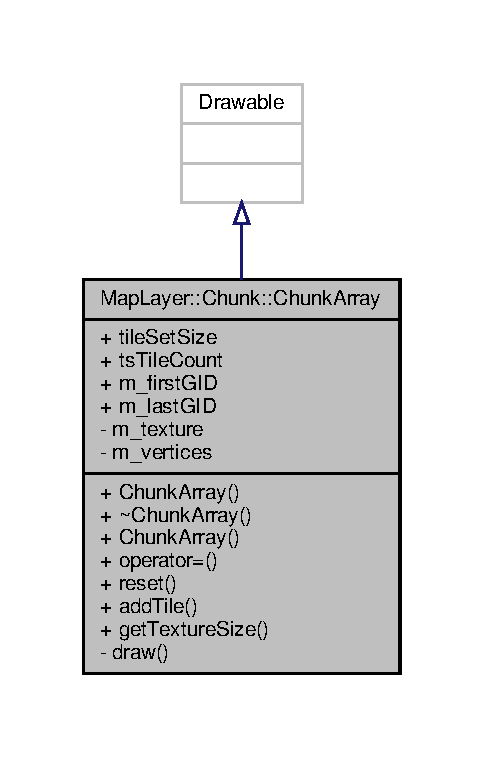
\includegraphics[width=232pt]{classMapLayer_1_1Chunk_1_1ChunkArray__inherit__graph}
\end{center}
\end{figure}


Collaboration diagram for Map\+Layer\+:\+:Chunk\+:\+:Chunk\+Array\+:
\nopagebreak
\begin{figure}[H]
\begin{center}
\leavevmode
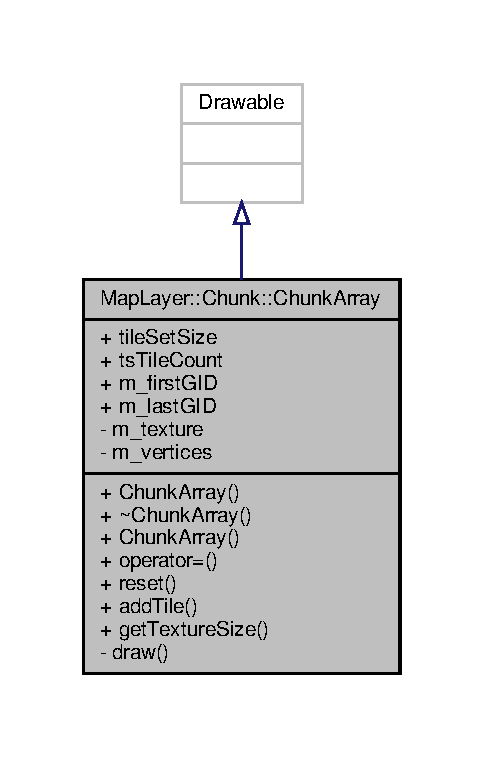
\includegraphics[width=232pt]{classMapLayer_1_1Chunk_1_1ChunkArray__coll__graph}
\end{center}
\end{figure}
\subsection*{Public Types}
\begin{DoxyCompactItemize}
\item 
using \hyperlink{classMapLayer_1_1Chunk_1_1ChunkArray_a6d944dee2fc89a76d7a252405e2732b0}{Ptr} = std\+::unique\+\_\+ptr$<$ \hyperlink{classMapLayer_1_1Chunk_1_1ChunkArray}{Chunk\+Array} $>$
\end{DoxyCompactItemize}
\subsection*{Public Member Functions}
\begin{DoxyCompactItemize}
\item 
\hyperlink{classMapLayer_1_1Chunk_1_1ChunkArray_a566f7f2c8c1fd2405ed8a359a9cf8717}{Chunk\+Array} (const sf\+::\+Texture \&t, const tmx\+::\+Tileset \&ts)
\item 
\hyperlink{classMapLayer_1_1Chunk_1_1ChunkArray_a032e0fa8a35d86815109eb0e1296c567}{$\sim$\+Chunk\+Array} ()=default
\item 
\hyperlink{classMapLayer_1_1Chunk_1_1ChunkArray_a85a82c50eae1a835b7a355813b560cbf}{Chunk\+Array} (const \hyperlink{classMapLayer_1_1Chunk_1_1ChunkArray}{Chunk\+Array} \&)=delete
\item 
\hyperlink{classMapLayer_1_1Chunk_1_1ChunkArray}{Chunk\+Array} \& \hyperlink{classMapLayer_1_1Chunk_1_1ChunkArray_ad5c7843e61bbddfb1be30ec93d75510f}{operator=} (const \hyperlink{classMapLayer_1_1Chunk_1_1ChunkArray}{Chunk\+Array} \&)=delete
\item 
void \hyperlink{classMapLayer_1_1Chunk_1_1ChunkArray_a4f93efce951889766d0336525e697cdd}{reset} ()
\item 
void \hyperlink{classMapLayer_1_1Chunk_1_1ChunkArray_a5d3cc7cca03c66402b6a73978e1440dc}{add\+Tile} (const \hyperlink{classMapLayer_1_1Chunk_a2137a288bfd4120eb3e4db5934b802f3}{Chunk\+::\+Tile} \&tile)
\item 
sf\+::\+Vector2u \hyperlink{classMapLayer_1_1Chunk_1_1ChunkArray_a6de1bdb0370138d0b63b8817da6fb2a2}{get\+Texture\+Size} () const
\end{DoxyCompactItemize}
\subsection*{Public Attributes}
\begin{DoxyCompactItemize}
\item 
tmx\+::\+Vector2u \hyperlink{classMapLayer_1_1Chunk_1_1ChunkArray_a2338cdb0f900b21dd175ac86f7d4d984}{tile\+Set\+Size}
\item 
sf\+::\+Vector2u \hyperlink{classMapLayer_1_1Chunk_1_1ChunkArray_a2248df4d35f691b2b2afe3aeb02f50ed}{ts\+Tile\+Count}
\item 
std\+::uint32\+\_\+t \hyperlink{classMapLayer_1_1Chunk_1_1ChunkArray_a5f4d6066ddf867552b992d8215fbffcb}{m\+\_\+first\+G\+ID}
\item 
std\+::uint32\+\_\+t \hyperlink{classMapLayer_1_1Chunk_1_1ChunkArray_a02890e0578dbc2550e74ac1734b6c608}{m\+\_\+last\+G\+ID}
\end{DoxyCompactItemize}
\subsection*{Private Member Functions}
\begin{DoxyCompactItemize}
\item 
void \hyperlink{classMapLayer_1_1Chunk_1_1ChunkArray_a9eb79b994907878e26c521a4d0c111b4}{draw} (sf\+::\+Render\+Target \&rt, sf\+::\+Render\+States states) const override
\end{DoxyCompactItemize}
\subsection*{Private Attributes}
\begin{DoxyCompactItemize}
\item 
const sf\+::\+Texture \& \hyperlink{classMapLayer_1_1Chunk_1_1ChunkArray_a84294fb3f90d1363a3095a978f0b89f8}{m\+\_\+texture}
\item 
std\+::vector$<$ sf\+::\+Vertex $>$ \hyperlink{classMapLayer_1_1Chunk_1_1ChunkArray_a43fbfdccc94de7aa7e3f822d93789dc6}{m\+\_\+vertices}
\end{DoxyCompactItemize}


\subsection{Member Typedef Documentation}
\mbox{\Hypertarget{classMapLayer_1_1Chunk_1_1ChunkArray_a6d944dee2fc89a76d7a252405e2732b0}\label{classMapLayer_1_1Chunk_1_1ChunkArray_a6d944dee2fc89a76d7a252405e2732b0}} 
\index{Map\+Layer\+::\+Chunk\+::\+Chunk\+Array@{Map\+Layer\+::\+Chunk\+::\+Chunk\+Array}!Ptr@{Ptr}}
\index{Ptr@{Ptr}!Map\+Layer\+::\+Chunk\+::\+Chunk\+Array@{Map\+Layer\+::\+Chunk\+::\+Chunk\+Array}}
\subsubsection{\texorpdfstring{Ptr}{Ptr}}
{\footnotesize\ttfamily using \hyperlink{classMapLayer_1_1Chunk_1_1ChunkArray_a6d944dee2fc89a76d7a252405e2732b0}{Map\+Layer\+::\+Chunk\+::\+Chunk\+Array\+::\+Ptr} =  std\+::unique\+\_\+ptr$<$\hyperlink{classMapLayer_1_1Chunk_1_1ChunkArray}{Chunk\+Array}$>$}



\subsection{Constructor \& Destructor Documentation}
\mbox{\Hypertarget{classMapLayer_1_1Chunk_1_1ChunkArray_a566f7f2c8c1fd2405ed8a359a9cf8717}\label{classMapLayer_1_1Chunk_1_1ChunkArray_a566f7f2c8c1fd2405ed8a359a9cf8717}} 
\index{Map\+Layer\+::\+Chunk\+::\+Chunk\+Array@{Map\+Layer\+::\+Chunk\+::\+Chunk\+Array}!Chunk\+Array@{Chunk\+Array}}
\index{Chunk\+Array@{Chunk\+Array}!Map\+Layer\+::\+Chunk\+::\+Chunk\+Array@{Map\+Layer\+::\+Chunk\+::\+Chunk\+Array}}
\subsubsection{\texorpdfstring{Chunk\+Array()}{ChunkArray()}\hspace{0.1cm}{\footnotesize\ttfamily [1/2]}}
{\footnotesize\ttfamily Map\+Layer\+::\+Chunk\+::\+Chunk\+Array\+::\+Chunk\+Array (\begin{DoxyParamCaption}\item[{const sf\+::\+Texture \&}]{t,  }\item[{const tmx\+::\+Tileset \&}]{ts }\end{DoxyParamCaption})\hspace{0.3cm}{\ttfamily [inline]}, {\ttfamily [explicit]}}

\mbox{\Hypertarget{classMapLayer_1_1Chunk_1_1ChunkArray_a032e0fa8a35d86815109eb0e1296c567}\label{classMapLayer_1_1Chunk_1_1ChunkArray_a032e0fa8a35d86815109eb0e1296c567}} 
\index{Map\+Layer\+::\+Chunk\+::\+Chunk\+Array@{Map\+Layer\+::\+Chunk\+::\+Chunk\+Array}!````~Chunk\+Array@{$\sim$\+Chunk\+Array}}
\index{````~Chunk\+Array@{$\sim$\+Chunk\+Array}!Map\+Layer\+::\+Chunk\+::\+Chunk\+Array@{Map\+Layer\+::\+Chunk\+::\+Chunk\+Array}}
\subsubsection{\texorpdfstring{$\sim$\+Chunk\+Array()}{~ChunkArray()}}
{\footnotesize\ttfamily Map\+Layer\+::\+Chunk\+::\+Chunk\+Array\+::$\sim$\+Chunk\+Array (\begin{DoxyParamCaption}{ }\end{DoxyParamCaption})\hspace{0.3cm}{\ttfamily [default]}}

\mbox{\Hypertarget{classMapLayer_1_1Chunk_1_1ChunkArray_a85a82c50eae1a835b7a355813b560cbf}\label{classMapLayer_1_1Chunk_1_1ChunkArray_a85a82c50eae1a835b7a355813b560cbf}} 
\index{Map\+Layer\+::\+Chunk\+::\+Chunk\+Array@{Map\+Layer\+::\+Chunk\+::\+Chunk\+Array}!Chunk\+Array@{Chunk\+Array}}
\index{Chunk\+Array@{Chunk\+Array}!Map\+Layer\+::\+Chunk\+::\+Chunk\+Array@{Map\+Layer\+::\+Chunk\+::\+Chunk\+Array}}
\subsubsection{\texorpdfstring{Chunk\+Array()}{ChunkArray()}\hspace{0.1cm}{\footnotesize\ttfamily [2/2]}}
{\footnotesize\ttfamily Map\+Layer\+::\+Chunk\+::\+Chunk\+Array\+::\+Chunk\+Array (\begin{DoxyParamCaption}\item[{const \hyperlink{classMapLayer_1_1Chunk_1_1ChunkArray}{Chunk\+Array} \&}]{ }\end{DoxyParamCaption})\hspace{0.3cm}{\ttfamily [delete]}}



\subsection{Member Function Documentation}
\mbox{\Hypertarget{classMapLayer_1_1Chunk_1_1ChunkArray_a5d3cc7cca03c66402b6a73978e1440dc}\label{classMapLayer_1_1Chunk_1_1ChunkArray_a5d3cc7cca03c66402b6a73978e1440dc}} 
\index{Map\+Layer\+::\+Chunk\+::\+Chunk\+Array@{Map\+Layer\+::\+Chunk\+::\+Chunk\+Array}!add\+Tile@{add\+Tile}}
\index{add\+Tile@{add\+Tile}!Map\+Layer\+::\+Chunk\+::\+Chunk\+Array@{Map\+Layer\+::\+Chunk\+::\+Chunk\+Array}}
\subsubsection{\texorpdfstring{add\+Tile()}{addTile()}}
{\footnotesize\ttfamily void Map\+Layer\+::\+Chunk\+::\+Chunk\+Array\+::add\+Tile (\begin{DoxyParamCaption}\item[{const \hyperlink{classMapLayer_1_1Chunk_a2137a288bfd4120eb3e4db5934b802f3}{Chunk\+::\+Tile} \&}]{tile }\end{DoxyParamCaption})\hspace{0.3cm}{\ttfamily [inline]}}

\mbox{\Hypertarget{classMapLayer_1_1Chunk_1_1ChunkArray_a9eb79b994907878e26c521a4d0c111b4}\label{classMapLayer_1_1Chunk_1_1ChunkArray_a9eb79b994907878e26c521a4d0c111b4}} 
\index{Map\+Layer\+::\+Chunk\+::\+Chunk\+Array@{Map\+Layer\+::\+Chunk\+::\+Chunk\+Array}!draw@{draw}}
\index{draw@{draw}!Map\+Layer\+::\+Chunk\+::\+Chunk\+Array@{Map\+Layer\+::\+Chunk\+::\+Chunk\+Array}}
\subsubsection{\texorpdfstring{draw()}{draw()}}
{\footnotesize\ttfamily void Map\+Layer\+::\+Chunk\+::\+Chunk\+Array\+::draw (\begin{DoxyParamCaption}\item[{sf\+::\+Render\+Target \&}]{rt,  }\item[{sf\+::\+Render\+States}]{states }\end{DoxyParamCaption}) const\hspace{0.3cm}{\ttfamily [inline]}, {\ttfamily [override]}, {\ttfamily [private]}}

\mbox{\Hypertarget{classMapLayer_1_1Chunk_1_1ChunkArray_a6de1bdb0370138d0b63b8817da6fb2a2}\label{classMapLayer_1_1Chunk_1_1ChunkArray_a6de1bdb0370138d0b63b8817da6fb2a2}} 
\index{Map\+Layer\+::\+Chunk\+::\+Chunk\+Array@{Map\+Layer\+::\+Chunk\+::\+Chunk\+Array}!get\+Texture\+Size@{get\+Texture\+Size}}
\index{get\+Texture\+Size@{get\+Texture\+Size}!Map\+Layer\+::\+Chunk\+::\+Chunk\+Array@{Map\+Layer\+::\+Chunk\+::\+Chunk\+Array}}
\subsubsection{\texorpdfstring{get\+Texture\+Size()}{getTextureSize()}}
{\footnotesize\ttfamily sf\+::\+Vector2u Map\+Layer\+::\+Chunk\+::\+Chunk\+Array\+::get\+Texture\+Size (\begin{DoxyParamCaption}{ }\end{DoxyParamCaption}) const\hspace{0.3cm}{\ttfamily [inline]}}

\mbox{\Hypertarget{classMapLayer_1_1Chunk_1_1ChunkArray_ad5c7843e61bbddfb1be30ec93d75510f}\label{classMapLayer_1_1Chunk_1_1ChunkArray_ad5c7843e61bbddfb1be30ec93d75510f}} 
\index{Map\+Layer\+::\+Chunk\+::\+Chunk\+Array@{Map\+Layer\+::\+Chunk\+::\+Chunk\+Array}!operator=@{operator=}}
\index{operator=@{operator=}!Map\+Layer\+::\+Chunk\+::\+Chunk\+Array@{Map\+Layer\+::\+Chunk\+::\+Chunk\+Array}}
\subsubsection{\texorpdfstring{operator=()}{operator=()}}
{\footnotesize\ttfamily \hyperlink{classMapLayer_1_1Chunk_1_1ChunkArray}{Chunk\+Array}\& Map\+Layer\+::\+Chunk\+::\+Chunk\+Array\+::operator= (\begin{DoxyParamCaption}\item[{const \hyperlink{classMapLayer_1_1Chunk_1_1ChunkArray}{Chunk\+Array} \&}]{ }\end{DoxyParamCaption})\hspace{0.3cm}{\ttfamily [delete]}}

\mbox{\Hypertarget{classMapLayer_1_1Chunk_1_1ChunkArray_a4f93efce951889766d0336525e697cdd}\label{classMapLayer_1_1Chunk_1_1ChunkArray_a4f93efce951889766d0336525e697cdd}} 
\index{Map\+Layer\+::\+Chunk\+::\+Chunk\+Array@{Map\+Layer\+::\+Chunk\+::\+Chunk\+Array}!reset@{reset}}
\index{reset@{reset}!Map\+Layer\+::\+Chunk\+::\+Chunk\+Array@{Map\+Layer\+::\+Chunk\+::\+Chunk\+Array}}
\subsubsection{\texorpdfstring{reset()}{reset()}}
{\footnotesize\ttfamily void Map\+Layer\+::\+Chunk\+::\+Chunk\+Array\+::reset (\begin{DoxyParamCaption}{ }\end{DoxyParamCaption})\hspace{0.3cm}{\ttfamily [inline]}}



\subsection{Member Data Documentation}
\mbox{\Hypertarget{classMapLayer_1_1Chunk_1_1ChunkArray_a5f4d6066ddf867552b992d8215fbffcb}\label{classMapLayer_1_1Chunk_1_1ChunkArray_a5f4d6066ddf867552b992d8215fbffcb}} 
\index{Map\+Layer\+::\+Chunk\+::\+Chunk\+Array@{Map\+Layer\+::\+Chunk\+::\+Chunk\+Array}!m\+\_\+first\+G\+ID@{m\+\_\+first\+G\+ID}}
\index{m\+\_\+first\+G\+ID@{m\+\_\+first\+G\+ID}!Map\+Layer\+::\+Chunk\+::\+Chunk\+Array@{Map\+Layer\+::\+Chunk\+::\+Chunk\+Array}}
\subsubsection{\texorpdfstring{m\+\_\+first\+G\+ID}{m\_firstGID}}
{\footnotesize\ttfamily std\+::uint32\+\_\+t Map\+Layer\+::\+Chunk\+::\+Chunk\+Array\+::m\+\_\+first\+G\+ID}

\mbox{\Hypertarget{classMapLayer_1_1Chunk_1_1ChunkArray_a02890e0578dbc2550e74ac1734b6c608}\label{classMapLayer_1_1Chunk_1_1ChunkArray_a02890e0578dbc2550e74ac1734b6c608}} 
\index{Map\+Layer\+::\+Chunk\+::\+Chunk\+Array@{Map\+Layer\+::\+Chunk\+::\+Chunk\+Array}!m\+\_\+last\+G\+ID@{m\+\_\+last\+G\+ID}}
\index{m\+\_\+last\+G\+ID@{m\+\_\+last\+G\+ID}!Map\+Layer\+::\+Chunk\+::\+Chunk\+Array@{Map\+Layer\+::\+Chunk\+::\+Chunk\+Array}}
\subsubsection{\texorpdfstring{m\+\_\+last\+G\+ID}{m\_lastGID}}
{\footnotesize\ttfamily std\+::uint32\+\_\+t Map\+Layer\+::\+Chunk\+::\+Chunk\+Array\+::m\+\_\+last\+G\+ID}

\mbox{\Hypertarget{classMapLayer_1_1Chunk_1_1ChunkArray_a84294fb3f90d1363a3095a978f0b89f8}\label{classMapLayer_1_1Chunk_1_1ChunkArray_a84294fb3f90d1363a3095a978f0b89f8}} 
\index{Map\+Layer\+::\+Chunk\+::\+Chunk\+Array@{Map\+Layer\+::\+Chunk\+::\+Chunk\+Array}!m\+\_\+texture@{m\+\_\+texture}}
\index{m\+\_\+texture@{m\+\_\+texture}!Map\+Layer\+::\+Chunk\+::\+Chunk\+Array@{Map\+Layer\+::\+Chunk\+::\+Chunk\+Array}}
\subsubsection{\texorpdfstring{m\+\_\+texture}{m\_texture}}
{\footnotesize\ttfamily const sf\+::\+Texture\& Map\+Layer\+::\+Chunk\+::\+Chunk\+Array\+::m\+\_\+texture\hspace{0.3cm}{\ttfamily [private]}}

\mbox{\Hypertarget{classMapLayer_1_1Chunk_1_1ChunkArray_a43fbfdccc94de7aa7e3f822d93789dc6}\label{classMapLayer_1_1Chunk_1_1ChunkArray_a43fbfdccc94de7aa7e3f822d93789dc6}} 
\index{Map\+Layer\+::\+Chunk\+::\+Chunk\+Array@{Map\+Layer\+::\+Chunk\+::\+Chunk\+Array}!m\+\_\+vertices@{m\+\_\+vertices}}
\index{m\+\_\+vertices@{m\+\_\+vertices}!Map\+Layer\+::\+Chunk\+::\+Chunk\+Array@{Map\+Layer\+::\+Chunk\+::\+Chunk\+Array}}
\subsubsection{\texorpdfstring{m\+\_\+vertices}{m\_vertices}}
{\footnotesize\ttfamily std\+::vector$<$sf\+::\+Vertex$>$ Map\+Layer\+::\+Chunk\+::\+Chunk\+Array\+::m\+\_\+vertices\hspace{0.3cm}{\ttfamily [private]}}

\mbox{\Hypertarget{classMapLayer_1_1Chunk_1_1ChunkArray_a2338cdb0f900b21dd175ac86f7d4d984}\label{classMapLayer_1_1Chunk_1_1ChunkArray_a2338cdb0f900b21dd175ac86f7d4d984}} 
\index{Map\+Layer\+::\+Chunk\+::\+Chunk\+Array@{Map\+Layer\+::\+Chunk\+::\+Chunk\+Array}!tile\+Set\+Size@{tile\+Set\+Size}}
\index{tile\+Set\+Size@{tile\+Set\+Size}!Map\+Layer\+::\+Chunk\+::\+Chunk\+Array@{Map\+Layer\+::\+Chunk\+::\+Chunk\+Array}}
\subsubsection{\texorpdfstring{tile\+Set\+Size}{tileSetSize}}
{\footnotesize\ttfamily tmx\+::\+Vector2u Map\+Layer\+::\+Chunk\+::\+Chunk\+Array\+::tile\+Set\+Size}

\mbox{\Hypertarget{classMapLayer_1_1Chunk_1_1ChunkArray_a2248df4d35f691b2b2afe3aeb02f50ed}\label{classMapLayer_1_1Chunk_1_1ChunkArray_a2248df4d35f691b2b2afe3aeb02f50ed}} 
\index{Map\+Layer\+::\+Chunk\+::\+Chunk\+Array@{Map\+Layer\+::\+Chunk\+::\+Chunk\+Array}!ts\+Tile\+Count@{ts\+Tile\+Count}}
\index{ts\+Tile\+Count@{ts\+Tile\+Count}!Map\+Layer\+::\+Chunk\+::\+Chunk\+Array@{Map\+Layer\+::\+Chunk\+::\+Chunk\+Array}}
\subsubsection{\texorpdfstring{ts\+Tile\+Count}{tsTileCount}}
{\footnotesize\ttfamily sf\+::\+Vector2u Map\+Layer\+::\+Chunk\+::\+Chunk\+Array\+::ts\+Tile\+Count}



The documentation for this class was generated from the following file\+:\begin{DoxyCompactItemize}
\item 
/mnt/hdd/\+C0de/smart\+\_\+engine/include/\hyperlink{SFMLOrthogonalLayer_8hpp}{S\+F\+M\+L\+Orthogonal\+Layer.\+hpp}\end{DoxyCompactItemize}

\hypertarget{classEntity}{}\section{Entity Class Reference}
\label{classEntity}\index{Entity@{Entity}}


{\ttfamily \#include $<$entity.\+h$>$}



Inheritance diagram for Entity\+:
\nopagebreak
\begin{figure}[H]
\begin{center}
\leavevmode
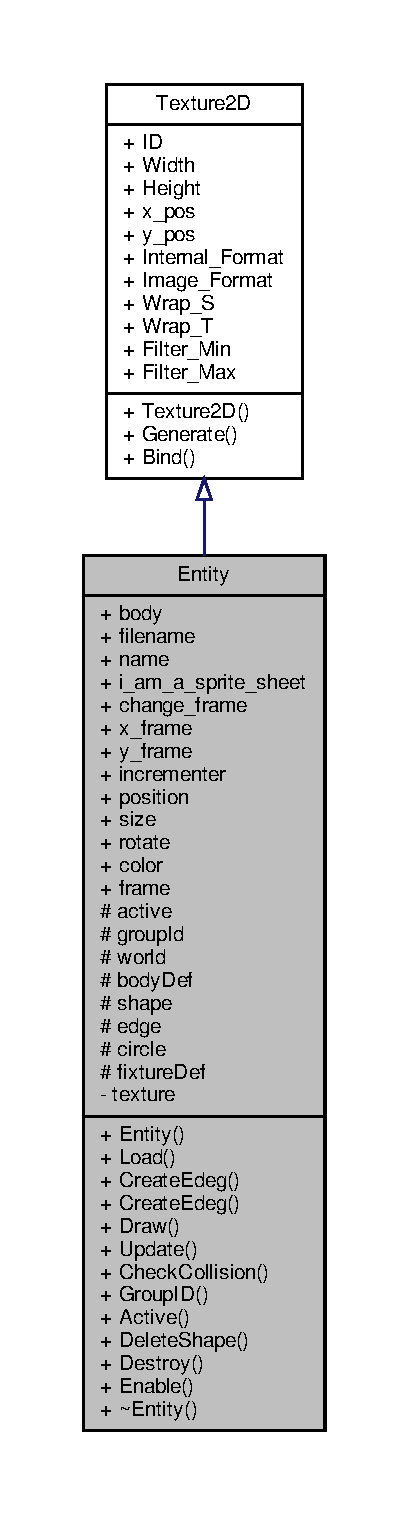
\includegraphics[height=550pt]{classEntity__inherit__graph}
\end{center}
\end{figure}


Collaboration diagram for Entity\+:
\nopagebreak
\begin{figure}[H]
\begin{center}
\leavevmode
\includegraphics[height=550pt]{classEntity__coll__graph}
\end{center}
\end{figure}
\subsection*{Public Member Functions}
\begin{DoxyCompactItemize}
\item 
\hyperlink{classEntity_a921d3ec8d8b5f758f82af131847b6edb}{Entity} (std\+::shared\+\_\+ptr$<$ b2\+World $>$ \hyperlink{classEntity_a83af93b5af6170706ebedb406caae509}{world})
\item 
void \hyperlink{classEntity_a2102aef307a324ec71ab31de73e52ee9}{Load} (const std\+::string \hyperlink{classEntity_a6a4de89770f168dbe6134fec0c5f2ad1}{filename}, bool dynamic, const std\+::string key, bool sprite\+\_\+sheet, bool change\+\_\+frames, bool set\+\_\+physics, const unsigned int x, const unsigned int y, float \hyperlink{classEntity_a97cf0dd2b95f85c3f611c30f7a9fbf68}{incrementer}, glm\+::vec2 pos, glm\+::vec2 \hyperlink{classEntity_a4cac664de0560de978d85456f5426baa}{size}, float rotation, glm\+::vec3 \hyperlink{classEntity_a688dc0de5b453c60a542a4dbdf06322e}{color})
\item 
void \hyperlink{classEntity_a7fefffa6364b37cda22e713ab316fcc5}{Create\+Edeg} (float, float, float, float)
\item 
void \hyperlink{classEntity_af26655d5ca92e2a075940fc17fe68b1f}{Create\+Edeg} ()
\item 
void \hyperlink{classEntity_af0befbcbae6115851975d763e7dda312}{Draw} ()
\item 
bool \hyperlink{classEntity_a4417060da59c34999fe3f0b912cacd16}{Update} ()
\item 
bool \hyperlink{classEntity_a3c39519c4beb655b319767606413b7d6}{Check\+Collision} (\hyperlink{classEntity}{Entity} $\ast$entity)
\item 
int \hyperlink{classEntity_af4549ca1382aea2706101bc26b749d47}{Group\+ID} ()
\item 
int \hyperlink{classEntity_ae71d6f69f40deb56a6357bb4bf750091}{Active} ()
\item 
void \hyperlink{classEntity_a5910a6f56586f89d31b34f175ad29ea1}{Delete\+Shape} ()
\item 
void \hyperlink{classEntity_aa75151fc607686b42d27f8c3ba73143d}{Destroy} ()
\item 
void \hyperlink{classEntity_ad940b54ddb93e1b2cc72012589576478}{Enable} ()
\item 
\hyperlink{classEntity_adf6d3f7cb1b2ba029b6b048a395cc8ae}{$\sim$\+Entity} ()
\end{DoxyCompactItemize}
\subsection*{Public Attributes}
\begin{DoxyCompactItemize}
\item 
b2\+Body $\ast$ \hyperlink{classEntity_a2b6ad094dc400a22a508aaccd956f9fd}{body}
\item 
std\+::string \hyperlink{classEntity_a6a4de89770f168dbe6134fec0c5f2ad1}{filename}
\item 
std\+::string \hyperlink{classEntity_a931b21fbdebb1a5963b4bcab5df128f5}{name}
\item 
bool \hyperlink{classEntity_a173e8f73ab7942235c1c3a4a1f4c40b0}{i\+\_\+am\+\_\+a\+\_\+sprite\+\_\+sheet}
\item 
bool \hyperlink{classEntity_a319afd83a878db68e6de473418e9a1f3}{change\+\_\+frame}
\item 
unsigned int \hyperlink{classEntity_ae38d1819b321f27f5771bf6d21af3c6f}{x\+\_\+frame}
\item 
unsigned int \hyperlink{classEntity_a778391410b1ff1f89fd6f06c8b636072}{y\+\_\+frame}
\item 
float \hyperlink{classEntity_a97cf0dd2b95f85c3f611c30f7a9fbf68}{incrementer}
\item 
glm\+::vec2 \hyperlink{classEntity_a01a4c7bdc113c1cbec8326a3f8d7d452}{position}
\item 
glm\+::vec2 \hyperlink{classEntity_a4cac664de0560de978d85456f5426baa}{size} = glm\+::vec2(10.\+0f, 10.\+0f)
\item 
float \hyperlink{classEntity_ad0baaae3c8c1c760bceb2e2c8676842b}{rotate} = 0.\+0f
\item 
glm\+::vec3 \hyperlink{classEntity_a688dc0de5b453c60a542a4dbdf06322e}{color} = glm\+::vec3(1.\+0f)
\item 
int \hyperlink{classEntity_a806d820393849740ea10917ef5a7f427}{frame}
\end{DoxyCompactItemize}
\subsection*{Protected Attributes}
\begin{DoxyCompactItemize}
\item 
int \hyperlink{classEntity_aeb5d37f9e2951abb86bb82f1875438a7}{active}
\item 
int \hyperlink{classEntity_a3caf6ab17eedfd51abe34e636ef9511f}{group\+Id}
\item 
std\+::shared\+\_\+ptr$<$ b2\+World $>$ \hyperlink{classEntity_a83af93b5af6170706ebedb406caae509}{world}
\item 
b2\+Body\+Def $\ast$ \hyperlink{classEntity_a84add379cdb92213cb236ea740a9c255}{body\+Def}
\item 
b2\+Polygon\+Shape $\ast$ \hyperlink{classEntity_ab8d8aadc7e72bc705718982d4804f491}{shape}
\item 
b2\+Edge\+Shape $\ast$ \hyperlink{classEntity_a0da995c93abd009e3a35bfb173526eaf}{edge}
\item 
b2\+Circle\+Shape $\ast$ \hyperlink{classEntity_aff413506dfd893191af8732c9acf28b0}{circle}
\item 
b2\+Fixture\+Def $\ast$ \hyperlink{classEntity_ac4eb27d6eca629016575130b40273a4b}{fixture\+Def}
\end{DoxyCompactItemize}
\subsection*{Private Attributes}
\begin{DoxyCompactItemize}
\item 
\hyperlink{classTexture2D}{Texture2D} $\ast$ \hyperlink{classEntity_a890913a7b3f4099622615ef0d589df77}{texture}
\end{DoxyCompactItemize}


\subsection{Constructor \& Destructor Documentation}
\mbox{\Hypertarget{classEntity_a921d3ec8d8b5f758f82af131847b6edb}\label{classEntity_a921d3ec8d8b5f758f82af131847b6edb}} 
\index{Entity@{Entity}!Entity@{Entity}}
\index{Entity@{Entity}!Entity@{Entity}}
\subsubsection{\texorpdfstring{Entity()}{Entity()}}
{\footnotesize\ttfamily Entity\+::\+Entity (\begin{DoxyParamCaption}\item[{std\+::shared\+\_\+ptr$<$ b2\+World $>$}]{world }\end{DoxyParamCaption})}

\mbox{\Hypertarget{classEntity_adf6d3f7cb1b2ba029b6b048a395cc8ae}\label{classEntity_adf6d3f7cb1b2ba029b6b048a395cc8ae}} 
\index{Entity@{Entity}!````~Entity@{$\sim$\+Entity}}
\index{````~Entity@{$\sim$\+Entity}!Entity@{Entity}}
\subsubsection{\texorpdfstring{$\sim$\+Entity()}{~Entity()}}
{\footnotesize\ttfamily Entity\+::$\sim$\+Entity (\begin{DoxyParamCaption}{ }\end{DoxyParamCaption})}



\subsection{Member Function Documentation}
\mbox{\Hypertarget{classEntity_ae71d6f69f40deb56a6357bb4bf750091}\label{classEntity_ae71d6f69f40deb56a6357bb4bf750091}} 
\index{Entity@{Entity}!Active@{Active}}
\index{Active@{Active}!Entity@{Entity}}
\subsubsection{\texorpdfstring{Active()}{Active()}}
{\footnotesize\ttfamily int Entity\+::\+Active (\begin{DoxyParamCaption}{ }\end{DoxyParamCaption})\hspace{0.3cm}{\ttfamily [inline]}}

\mbox{\Hypertarget{classEntity_a3c39519c4beb655b319767606413b7d6}\label{classEntity_a3c39519c4beb655b319767606413b7d6}} 
\index{Entity@{Entity}!Check\+Collision@{Check\+Collision}}
\index{Check\+Collision@{Check\+Collision}!Entity@{Entity}}
\subsubsection{\texorpdfstring{Check\+Collision()}{CheckCollision()}}
{\footnotesize\ttfamily bool Entity\+::\+Check\+Collision (\begin{DoxyParamCaption}\item[{\hyperlink{classEntity}{Entity} $\ast$}]{entity }\end{DoxyParamCaption})}

\mbox{\Hypertarget{classEntity_a7fefffa6364b37cda22e713ab316fcc5}\label{classEntity_a7fefffa6364b37cda22e713ab316fcc5}} 
\index{Entity@{Entity}!Create\+Edeg@{Create\+Edeg}}
\index{Create\+Edeg@{Create\+Edeg}!Entity@{Entity}}
\subsubsection{\texorpdfstring{Create\+Edeg()}{CreateEdeg()}\hspace{0.1cm}{\footnotesize\ttfamily [1/2]}}
{\footnotesize\ttfamily void Entity\+::\+Create\+Edeg (\begin{DoxyParamCaption}\item[{float}]{x\+\_\+point\+\_\+origin,  }\item[{float}]{y\+\_\+point\+\_\+origin,  }\item[{float}]{x\+\_\+point\+\_\+dest,  }\item[{float}]{y\+\_\+point\+\_\+dest }\end{DoxyParamCaption})}

\mbox{\Hypertarget{classEntity_af26655d5ca92e2a075940fc17fe68b1f}\label{classEntity_af26655d5ca92e2a075940fc17fe68b1f}} 
\index{Entity@{Entity}!Create\+Edeg@{Create\+Edeg}}
\index{Create\+Edeg@{Create\+Edeg}!Entity@{Entity}}
\subsubsection{\texorpdfstring{Create\+Edeg()}{CreateEdeg()}\hspace{0.1cm}{\footnotesize\ttfamily [2/2]}}
{\footnotesize\ttfamily void Entity\+::\+Create\+Edeg (\begin{DoxyParamCaption}{ }\end{DoxyParamCaption})}

\mbox{\Hypertarget{classEntity_a5910a6f56586f89d31b34f175ad29ea1}\label{classEntity_a5910a6f56586f89d31b34f175ad29ea1}} 
\index{Entity@{Entity}!Delete\+Shape@{Delete\+Shape}}
\index{Delete\+Shape@{Delete\+Shape}!Entity@{Entity}}
\subsubsection{\texorpdfstring{Delete\+Shape()}{DeleteShape()}}
{\footnotesize\ttfamily void Entity\+::\+Delete\+Shape (\begin{DoxyParamCaption}{ }\end{DoxyParamCaption})\hspace{0.3cm}{\ttfamily [inline]}}

\mbox{\Hypertarget{classEntity_aa75151fc607686b42d27f8c3ba73143d}\label{classEntity_aa75151fc607686b42d27f8c3ba73143d}} 
\index{Entity@{Entity}!Destroy@{Destroy}}
\index{Destroy@{Destroy}!Entity@{Entity}}
\subsubsection{\texorpdfstring{Destroy()}{Destroy()}}
{\footnotesize\ttfamily void Entity\+::\+Destroy (\begin{DoxyParamCaption}{ }\end{DoxyParamCaption})}

\mbox{\Hypertarget{classEntity_af0befbcbae6115851975d763e7dda312}\label{classEntity_af0befbcbae6115851975d763e7dda312}} 
\index{Entity@{Entity}!Draw@{Draw}}
\index{Draw@{Draw}!Entity@{Entity}}
\subsubsection{\texorpdfstring{Draw()}{Draw()}}
{\footnotesize\ttfamily void Entity\+::\+Draw (\begin{DoxyParamCaption}{ }\end{DoxyParamCaption})}

\mbox{\Hypertarget{classEntity_ad940b54ddb93e1b2cc72012589576478}\label{classEntity_ad940b54ddb93e1b2cc72012589576478}} 
\index{Entity@{Entity}!Enable@{Enable}}
\index{Enable@{Enable}!Entity@{Entity}}
\subsubsection{\texorpdfstring{Enable()}{Enable()}}
{\footnotesize\ttfamily void Entity\+::\+Enable (\begin{DoxyParamCaption}{ }\end{DoxyParamCaption})}

\mbox{\Hypertarget{classEntity_af4549ca1382aea2706101bc26b749d47}\label{classEntity_af4549ca1382aea2706101bc26b749d47}} 
\index{Entity@{Entity}!Group\+ID@{Group\+ID}}
\index{Group\+ID@{Group\+ID}!Entity@{Entity}}
\subsubsection{\texorpdfstring{Group\+I\+D()}{GroupID()}}
{\footnotesize\ttfamily int Entity\+::\+Group\+ID (\begin{DoxyParamCaption}{ }\end{DoxyParamCaption})\hspace{0.3cm}{\ttfamily [inline]}}

\mbox{\Hypertarget{classEntity_a2102aef307a324ec71ab31de73e52ee9}\label{classEntity_a2102aef307a324ec71ab31de73e52ee9}} 
\index{Entity@{Entity}!Load@{Load}}
\index{Load@{Load}!Entity@{Entity}}
\subsubsection{\texorpdfstring{Load()}{Load()}}
{\footnotesize\ttfamily void Entity\+::\+Load (\begin{DoxyParamCaption}\item[{const std\+::string}]{filename,  }\item[{bool}]{dynamic,  }\item[{const std\+::string}]{key,  }\item[{bool}]{sprite\+\_\+sheet,  }\item[{bool}]{change\+\_\+frames,  }\item[{bool}]{set\+\_\+physics,  }\item[{const unsigned int}]{x,  }\item[{const unsigned int}]{y,  }\item[{float}]{incrementer,  }\item[{glm\+::vec2}]{pos,  }\item[{glm\+::vec2}]{size,  }\item[{float}]{rotation,  }\item[{glm\+::vec3}]{color }\end{DoxyParamCaption})}

\mbox{\Hypertarget{classEntity_a4417060da59c34999fe3f0b912cacd16}\label{classEntity_a4417060da59c34999fe3f0b912cacd16}} 
\index{Entity@{Entity}!Update@{Update}}
\index{Update@{Update}!Entity@{Entity}}
\subsubsection{\texorpdfstring{Update()}{Update()}}
{\footnotesize\ttfamily bool Entity\+::\+Update (\begin{DoxyParamCaption}{ }\end{DoxyParamCaption})}



\subsection{Member Data Documentation}
\mbox{\Hypertarget{classEntity_aeb5d37f9e2951abb86bb82f1875438a7}\label{classEntity_aeb5d37f9e2951abb86bb82f1875438a7}} 
\index{Entity@{Entity}!active@{active}}
\index{active@{active}!Entity@{Entity}}
\subsubsection{\texorpdfstring{active}{active}}
{\footnotesize\ttfamily int Entity\+::active\hspace{0.3cm}{\ttfamily [protected]}}

\mbox{\Hypertarget{classEntity_a2b6ad094dc400a22a508aaccd956f9fd}\label{classEntity_a2b6ad094dc400a22a508aaccd956f9fd}} 
\index{Entity@{Entity}!body@{body}}
\index{body@{body}!Entity@{Entity}}
\subsubsection{\texorpdfstring{body}{body}}
{\footnotesize\ttfamily b2\+Body$\ast$ Entity\+::body}

\mbox{\Hypertarget{classEntity_a84add379cdb92213cb236ea740a9c255}\label{classEntity_a84add379cdb92213cb236ea740a9c255}} 
\index{Entity@{Entity}!body\+Def@{body\+Def}}
\index{body\+Def@{body\+Def}!Entity@{Entity}}
\subsubsection{\texorpdfstring{body\+Def}{bodyDef}}
{\footnotesize\ttfamily b2\+Body\+Def$\ast$ Entity\+::body\+Def\hspace{0.3cm}{\ttfamily [protected]}}

\mbox{\Hypertarget{classEntity_a319afd83a878db68e6de473418e9a1f3}\label{classEntity_a319afd83a878db68e6de473418e9a1f3}} 
\index{Entity@{Entity}!change\+\_\+frame@{change\+\_\+frame}}
\index{change\+\_\+frame@{change\+\_\+frame}!Entity@{Entity}}
\subsubsection{\texorpdfstring{change\+\_\+frame}{change\_frame}}
{\footnotesize\ttfamily bool Entity\+::change\+\_\+frame}

\mbox{\Hypertarget{classEntity_aff413506dfd893191af8732c9acf28b0}\label{classEntity_aff413506dfd893191af8732c9acf28b0}} 
\index{Entity@{Entity}!circle@{circle}}
\index{circle@{circle}!Entity@{Entity}}
\subsubsection{\texorpdfstring{circle}{circle}}
{\footnotesize\ttfamily b2\+Circle\+Shape$\ast$ Entity\+::circle\hspace{0.3cm}{\ttfamily [protected]}}

\mbox{\Hypertarget{classEntity_a688dc0de5b453c60a542a4dbdf06322e}\label{classEntity_a688dc0de5b453c60a542a4dbdf06322e}} 
\index{Entity@{Entity}!color@{color}}
\index{color@{color}!Entity@{Entity}}
\subsubsection{\texorpdfstring{color}{color}}
{\footnotesize\ttfamily glm\+::vec3 Entity\+::color = glm\+::vec3(1.\+0f)}

\mbox{\Hypertarget{classEntity_a0da995c93abd009e3a35bfb173526eaf}\label{classEntity_a0da995c93abd009e3a35bfb173526eaf}} 
\index{Entity@{Entity}!edge@{edge}}
\index{edge@{edge}!Entity@{Entity}}
\subsubsection{\texorpdfstring{edge}{edge}}
{\footnotesize\ttfamily b2\+Edge\+Shape$\ast$ Entity\+::edge\hspace{0.3cm}{\ttfamily [protected]}}

\mbox{\Hypertarget{classEntity_a6a4de89770f168dbe6134fec0c5f2ad1}\label{classEntity_a6a4de89770f168dbe6134fec0c5f2ad1}} 
\index{Entity@{Entity}!filename@{filename}}
\index{filename@{filename}!Entity@{Entity}}
\subsubsection{\texorpdfstring{filename}{filename}}
{\footnotesize\ttfamily std\+::string Entity\+::filename}

\mbox{\Hypertarget{classEntity_ac4eb27d6eca629016575130b40273a4b}\label{classEntity_ac4eb27d6eca629016575130b40273a4b}} 
\index{Entity@{Entity}!fixture\+Def@{fixture\+Def}}
\index{fixture\+Def@{fixture\+Def}!Entity@{Entity}}
\subsubsection{\texorpdfstring{fixture\+Def}{fixtureDef}}
{\footnotesize\ttfamily b2\+Fixture\+Def$\ast$ Entity\+::fixture\+Def\hspace{0.3cm}{\ttfamily [protected]}}

\mbox{\Hypertarget{classEntity_a806d820393849740ea10917ef5a7f427}\label{classEntity_a806d820393849740ea10917ef5a7f427}} 
\index{Entity@{Entity}!frame@{frame}}
\index{frame@{frame}!Entity@{Entity}}
\subsubsection{\texorpdfstring{frame}{frame}}
{\footnotesize\ttfamily int Entity\+::frame}

\mbox{\Hypertarget{classEntity_a3caf6ab17eedfd51abe34e636ef9511f}\label{classEntity_a3caf6ab17eedfd51abe34e636ef9511f}} 
\index{Entity@{Entity}!group\+Id@{group\+Id}}
\index{group\+Id@{group\+Id}!Entity@{Entity}}
\subsubsection{\texorpdfstring{group\+Id}{groupId}}
{\footnotesize\ttfamily int Entity\+::group\+Id\hspace{0.3cm}{\ttfamily [protected]}}

\mbox{\Hypertarget{classEntity_a173e8f73ab7942235c1c3a4a1f4c40b0}\label{classEntity_a173e8f73ab7942235c1c3a4a1f4c40b0}} 
\index{Entity@{Entity}!i\+\_\+am\+\_\+a\+\_\+sprite\+\_\+sheet@{i\+\_\+am\+\_\+a\+\_\+sprite\+\_\+sheet}}
\index{i\+\_\+am\+\_\+a\+\_\+sprite\+\_\+sheet@{i\+\_\+am\+\_\+a\+\_\+sprite\+\_\+sheet}!Entity@{Entity}}
\subsubsection{\texorpdfstring{i\+\_\+am\+\_\+a\+\_\+sprite\+\_\+sheet}{i\_am\_a\_sprite\_sheet}}
{\footnotesize\ttfamily bool Entity\+::i\+\_\+am\+\_\+a\+\_\+sprite\+\_\+sheet}

\mbox{\Hypertarget{classEntity_a97cf0dd2b95f85c3f611c30f7a9fbf68}\label{classEntity_a97cf0dd2b95f85c3f611c30f7a9fbf68}} 
\index{Entity@{Entity}!incrementer@{incrementer}}
\index{incrementer@{incrementer}!Entity@{Entity}}
\subsubsection{\texorpdfstring{incrementer}{incrementer}}
{\footnotesize\ttfamily float Entity\+::incrementer}

\mbox{\Hypertarget{classEntity_a931b21fbdebb1a5963b4bcab5df128f5}\label{classEntity_a931b21fbdebb1a5963b4bcab5df128f5}} 
\index{Entity@{Entity}!name@{name}}
\index{name@{name}!Entity@{Entity}}
\subsubsection{\texorpdfstring{name}{name}}
{\footnotesize\ttfamily std\+::string Entity\+::name}

\mbox{\Hypertarget{classEntity_a01a4c7bdc113c1cbec8326a3f8d7d452}\label{classEntity_a01a4c7bdc113c1cbec8326a3f8d7d452}} 
\index{Entity@{Entity}!position@{position}}
\index{position@{position}!Entity@{Entity}}
\subsubsection{\texorpdfstring{position}{position}}
{\footnotesize\ttfamily glm\+::vec2 Entity\+::position}

\mbox{\Hypertarget{classEntity_ad0baaae3c8c1c760bceb2e2c8676842b}\label{classEntity_ad0baaae3c8c1c760bceb2e2c8676842b}} 
\index{Entity@{Entity}!rotate@{rotate}}
\index{rotate@{rotate}!Entity@{Entity}}
\subsubsection{\texorpdfstring{rotate}{rotate}}
{\footnotesize\ttfamily float Entity\+::rotate = 0.\+0f}

\mbox{\Hypertarget{classEntity_ab8d8aadc7e72bc705718982d4804f491}\label{classEntity_ab8d8aadc7e72bc705718982d4804f491}} 
\index{Entity@{Entity}!shape@{shape}}
\index{shape@{shape}!Entity@{Entity}}
\subsubsection{\texorpdfstring{shape}{shape}}
{\footnotesize\ttfamily b2\+Polygon\+Shape$\ast$ Entity\+::shape\hspace{0.3cm}{\ttfamily [protected]}}

\mbox{\Hypertarget{classEntity_a4cac664de0560de978d85456f5426baa}\label{classEntity_a4cac664de0560de978d85456f5426baa}} 
\index{Entity@{Entity}!size@{size}}
\index{size@{size}!Entity@{Entity}}
\subsubsection{\texorpdfstring{size}{size}}
{\footnotesize\ttfamily glm\+::vec2 Entity\+::size = glm\+::vec2(10.\+0f, 10.\+0f)}

\mbox{\Hypertarget{classEntity_a890913a7b3f4099622615ef0d589df77}\label{classEntity_a890913a7b3f4099622615ef0d589df77}} 
\index{Entity@{Entity}!texture@{texture}}
\index{texture@{texture}!Entity@{Entity}}
\subsubsection{\texorpdfstring{texture}{texture}}
{\footnotesize\ttfamily \hyperlink{classTexture2D}{Texture2D}$\ast$ Entity\+::texture\hspace{0.3cm}{\ttfamily [private]}}

\mbox{\Hypertarget{classEntity_a83af93b5af6170706ebedb406caae509}\label{classEntity_a83af93b5af6170706ebedb406caae509}} 
\index{Entity@{Entity}!world@{world}}
\index{world@{world}!Entity@{Entity}}
\subsubsection{\texorpdfstring{world}{world}}
{\footnotesize\ttfamily std\+::shared\+\_\+ptr$<$b2\+World$>$ Entity\+::world\hspace{0.3cm}{\ttfamily [protected]}}

\mbox{\Hypertarget{classEntity_ae38d1819b321f27f5771bf6d21af3c6f}\label{classEntity_ae38d1819b321f27f5771bf6d21af3c6f}} 
\index{Entity@{Entity}!x\+\_\+frame@{x\+\_\+frame}}
\index{x\+\_\+frame@{x\+\_\+frame}!Entity@{Entity}}
\subsubsection{\texorpdfstring{x\+\_\+frame}{x\_frame}}
{\footnotesize\ttfamily unsigned int Entity\+::x\+\_\+frame}

\mbox{\Hypertarget{classEntity_a778391410b1ff1f89fd6f06c8b636072}\label{classEntity_a778391410b1ff1f89fd6f06c8b636072}} 
\index{Entity@{Entity}!y\+\_\+frame@{y\+\_\+frame}}
\index{y\+\_\+frame@{y\+\_\+frame}!Entity@{Entity}}
\subsubsection{\texorpdfstring{y\+\_\+frame}{y\_frame}}
{\footnotesize\ttfamily unsigned int Entity\+::y\+\_\+frame}



The documentation for this class was generated from the following files\+:\begin{DoxyCompactItemize}
\item 
/mnt/hdd/\+C0de/smart\+\_\+engine/include/\hyperlink{entity_8h}{entity.\+h}\item 
/mnt/hdd/\+C0de/smart\+\_\+engine/src/\hyperlink{entity_8cpp}{entity.\+cpp}\end{DoxyCompactItemize}

\hypertarget{classEntityManager}{}\section{Entity\+Manager Class Reference}
\label{classEntityManager}\index{Entity\+Manager@{Entity\+Manager}}


{\ttfamily \#include $<$entity\+\_\+manager.\+h$>$}



Collaboration diagram for Entity\+Manager\+:
\nopagebreak
\begin{figure}[H]
\begin{center}
\leavevmode
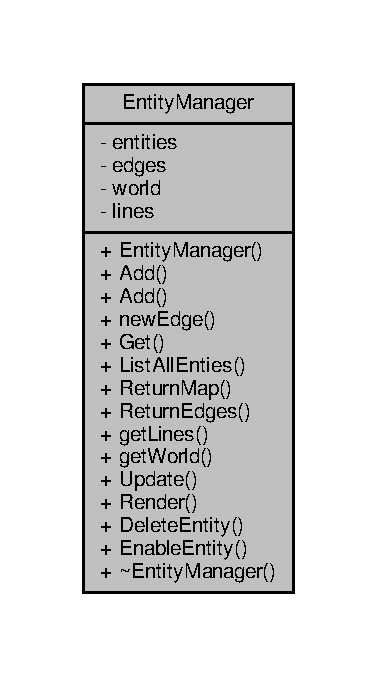
\includegraphics[width=181pt]{classEntityManager__coll__graph}
\end{center}
\end{figure}
\subsection*{Public Member Functions}
\begin{DoxyCompactItemize}
\item 
\hyperlink{classEntityManager_a7555637657d090171be6ceee8451de0a}{Entity\+Manager} ()
\item 
void \hyperlink{classEntityManager_a8724955e17641352db006a0050205d6d}{Add} (const std\+::string name, const std\+::string filename, bool dynamic, bool sprite\+\_\+sheet, bool change\+\_\+frames, bool set\+\_\+physics, const unsigned int x, const unsigned int y, float incrementer, glm\+::vec2 pos, glm\+::vec2 size, float rot, glm\+::vec3 color)
\item 
void \hyperlink{classEntityManager_a4d99f8a7949e50136c4665c2c53b31b3}{Add} (std\+::string name, std\+::string filename, bool dynamic, \hyperlink{entity__manager_8h_ad272ece963b9cc856176573f48fc6554}{shape\+\_\+options})
\item 
void \hyperlink{classEntityManager_a086131de1baa9936e0ffc6830bbe5039}{new\+Edge} (std\+::string, float x\+\_\+origin, float y\+\_\+origin, float x\+\_\+destination, float y\+\_\+destination, float color\+\_\+r=1.\+0f, float color\+\_\+g=1.\+0f, float color\+\_\+b=1.\+0f)
\item 
std\+::shared\+\_\+ptr$<$ \hyperlink{classEntity}{Entity} $>$ \hyperlink{classEntityManager_a8ece29270f575248ad03fad82f10b30b}{Get} (std\+::string name)
\item 
void \hyperlink{classEntityManager_ad16c34fbdcb0da9e9a3e1c59887d6e52}{List\+All\+Enties} ()
\item 
std\+::unordered\+\_\+map$<$ std\+::string, std\+::shared\+\_\+ptr$<$ \hyperlink{classEntity}{Entity} $>$ $>$ \hyperlink{classEntityManager_af1f233c05d50ee11a0c21cff1361e136}{Return\+Map} ()
\item 
std\+::unordered\+\_\+map$<$ std\+::string, std\+::shared\+\_\+ptr$<$ \hyperlink{classEntity}{Entity} $>$ $>$ \hyperlink{classEntityManager_a1b2f7559ef13126beebc8d0f5c32234c}{Return\+Edges} ()
\item 
std\+::vector$<$ std\+::shared\+\_\+ptr$<$ \hyperlink{classLine}{Line} $>$ $>$ \hyperlink{classEntityManager_a049eb8f4a36e91fe1b85d3fc8c7ef4e7}{get\+Lines} ()
\item 
std\+::shared\+\_\+ptr$<$ b2\+World $>$ \hyperlink{classEntityManager_ae684073af9ce6ab6e59cc9974c5f8a4c}{get\+World} ()
\item 
bool \hyperlink{classEntityManager_a1773a29978a78fc883eee2a037fab5bc}{Update} ()
\item 
void \hyperlink{classEntityManager_ad8bac9ea131d6b9dae9311dbc701d9ab}{Render} ()
\item 
void \hyperlink{classEntityManager_a9164014cb9331406a659d5ec61560f9d}{Delete\+Entity} ()
\item 
void \hyperlink{classEntityManager_a53286b6a783436258be418ec354dc584}{Enable\+Entity} ()
\item 
\hyperlink{classEntityManager_a71a36c9fb8d579a1a1ec108e0fccf175}{$\sim$\+Entity\+Manager} ()
\end{DoxyCompactItemize}
\subsection*{Private Attributes}
\begin{DoxyCompactItemize}
\item 
std\+::unordered\+\_\+map$<$ std\+::string, std\+::shared\+\_\+ptr$<$ \hyperlink{classEntity}{Entity} $>$ $>$ \hyperlink{classEntityManager_a9c442e6363c2269e9c95db90762367f3}{entities}
\item 
std\+::unordered\+\_\+map$<$ std\+::string, std\+::shared\+\_\+ptr$<$ \hyperlink{classEntity}{Entity} $>$ $>$ \hyperlink{classEntityManager_ae93f9beb111b9464327a70173411fda6}{edges}
\item 
std\+::shared\+\_\+ptr$<$ b2\+World $>$ \hyperlink{classEntityManager_ad2fdb512c0f27c7c60fbc9e6d2da4995}{world}
\item 
std\+::vector$<$ std\+::shared\+\_\+ptr$<$ \hyperlink{classLine}{Line} $>$ $>$ \hyperlink{classEntityManager_ae56b17654dc5fbdac4bb2359292cb369}{lines}
\end{DoxyCompactItemize}


\subsection{Constructor \& Destructor Documentation}
\mbox{\Hypertarget{classEntityManager_a7555637657d090171be6ceee8451de0a}\label{classEntityManager_a7555637657d090171be6ceee8451de0a}} 
\index{Entity\+Manager@{Entity\+Manager}!Entity\+Manager@{Entity\+Manager}}
\index{Entity\+Manager@{Entity\+Manager}!Entity\+Manager@{Entity\+Manager}}
\subsubsection{\texorpdfstring{Entity\+Manager()}{EntityManager()}}
{\footnotesize\ttfamily Entity\+Manager\+::\+Entity\+Manager (\begin{DoxyParamCaption}{ }\end{DoxyParamCaption})}

\mbox{\Hypertarget{classEntityManager_a71a36c9fb8d579a1a1ec108e0fccf175}\label{classEntityManager_a71a36c9fb8d579a1a1ec108e0fccf175}} 
\index{Entity\+Manager@{Entity\+Manager}!````~Entity\+Manager@{$\sim$\+Entity\+Manager}}
\index{````~Entity\+Manager@{$\sim$\+Entity\+Manager}!Entity\+Manager@{Entity\+Manager}}
\subsubsection{\texorpdfstring{$\sim$\+Entity\+Manager()}{~EntityManager()}}
{\footnotesize\ttfamily Entity\+Manager\+::$\sim$\+Entity\+Manager (\begin{DoxyParamCaption}{ }\end{DoxyParamCaption})}



\subsection{Member Function Documentation}
\mbox{\Hypertarget{classEntityManager_a8724955e17641352db006a0050205d6d}\label{classEntityManager_a8724955e17641352db006a0050205d6d}} 
\index{Entity\+Manager@{Entity\+Manager}!Add@{Add}}
\index{Add@{Add}!Entity\+Manager@{Entity\+Manager}}
\subsubsection{\texorpdfstring{Add()}{Add()}\hspace{0.1cm}{\footnotesize\ttfamily [1/2]}}
{\footnotesize\ttfamily void Entity\+Manager\+::\+Add (\begin{DoxyParamCaption}\item[{const std\+::string}]{name,  }\item[{const std\+::string}]{filename,  }\item[{bool}]{dynamic,  }\item[{bool}]{sprite\+\_\+sheet,  }\item[{bool}]{change\+\_\+frames,  }\item[{bool}]{set\+\_\+physics,  }\item[{const unsigned int}]{x,  }\item[{const unsigned int}]{y,  }\item[{float}]{incrementer,  }\item[{glm\+::vec2}]{pos,  }\item[{glm\+::vec2}]{size,  }\item[{float}]{rot,  }\item[{glm\+::vec3}]{color }\end{DoxyParamCaption})}

\mbox{\Hypertarget{classEntityManager_a4d99f8a7949e50136c4665c2c53b31b3}\label{classEntityManager_a4d99f8a7949e50136c4665c2c53b31b3}} 
\index{Entity\+Manager@{Entity\+Manager}!Add@{Add}}
\index{Add@{Add}!Entity\+Manager@{Entity\+Manager}}
\subsubsection{\texorpdfstring{Add()}{Add()}\hspace{0.1cm}{\footnotesize\ttfamily [2/2]}}
{\footnotesize\ttfamily void Entity\+Manager\+::\+Add (\begin{DoxyParamCaption}\item[{std\+::string}]{name,  }\item[{std\+::string}]{filename,  }\item[{bool}]{dynamic,  }\item[{\hyperlink{entity__manager_8h_ad272ece963b9cc856176573f48fc6554}{shape\+\_\+options}}]{shapes }\end{DoxyParamCaption})}

\mbox{\Hypertarget{classEntityManager_a9164014cb9331406a659d5ec61560f9d}\label{classEntityManager_a9164014cb9331406a659d5ec61560f9d}} 
\index{Entity\+Manager@{Entity\+Manager}!Delete\+Entity@{Delete\+Entity}}
\index{Delete\+Entity@{Delete\+Entity}!Entity\+Manager@{Entity\+Manager}}
\subsubsection{\texorpdfstring{Delete\+Entity()}{DeleteEntity()}}
{\footnotesize\ttfamily void Entity\+Manager\+::\+Delete\+Entity (\begin{DoxyParamCaption}{ }\end{DoxyParamCaption})}

\mbox{\Hypertarget{classEntityManager_a53286b6a783436258be418ec354dc584}\label{classEntityManager_a53286b6a783436258be418ec354dc584}} 
\index{Entity\+Manager@{Entity\+Manager}!Enable\+Entity@{Enable\+Entity}}
\index{Enable\+Entity@{Enable\+Entity}!Entity\+Manager@{Entity\+Manager}}
\subsubsection{\texorpdfstring{Enable\+Entity()}{EnableEntity()}}
{\footnotesize\ttfamily void Entity\+Manager\+::\+Enable\+Entity (\begin{DoxyParamCaption}{ }\end{DoxyParamCaption})}

\mbox{\Hypertarget{classEntityManager_a8ece29270f575248ad03fad82f10b30b}\label{classEntityManager_a8ece29270f575248ad03fad82f10b30b}} 
\index{Entity\+Manager@{Entity\+Manager}!Get@{Get}}
\index{Get@{Get}!Entity\+Manager@{Entity\+Manager}}
\subsubsection{\texorpdfstring{Get()}{Get()}}
{\footnotesize\ttfamily std\+::shared\+\_\+ptr$<$ \hyperlink{classEntity}{Entity} $>$ Entity\+Manager\+::\+Get (\begin{DoxyParamCaption}\item[{std\+::string}]{name }\end{DoxyParamCaption})}

\mbox{\Hypertarget{classEntityManager_a049eb8f4a36e91fe1b85d3fc8c7ef4e7}\label{classEntityManager_a049eb8f4a36e91fe1b85d3fc8c7ef4e7}} 
\index{Entity\+Manager@{Entity\+Manager}!get\+Lines@{get\+Lines}}
\index{get\+Lines@{get\+Lines}!Entity\+Manager@{Entity\+Manager}}
\subsubsection{\texorpdfstring{get\+Lines()}{getLines()}}
{\footnotesize\ttfamily std\+::vector$<$std\+::shared\+\_\+ptr$<$\hyperlink{classLine}{Line}$>$ $>$ Entity\+Manager\+::get\+Lines (\begin{DoxyParamCaption}{ }\end{DoxyParamCaption})\hspace{0.3cm}{\ttfamily [inline]}}

\mbox{\Hypertarget{classEntityManager_ae684073af9ce6ab6e59cc9974c5f8a4c}\label{classEntityManager_ae684073af9ce6ab6e59cc9974c5f8a4c}} 
\index{Entity\+Manager@{Entity\+Manager}!get\+World@{get\+World}}
\index{get\+World@{get\+World}!Entity\+Manager@{Entity\+Manager}}
\subsubsection{\texorpdfstring{get\+World()}{getWorld()}}
{\footnotesize\ttfamily std\+::shared\+\_\+ptr$<$b2\+World$>$ Entity\+Manager\+::get\+World (\begin{DoxyParamCaption}{ }\end{DoxyParamCaption})\hspace{0.3cm}{\ttfamily [inline]}}

\mbox{\Hypertarget{classEntityManager_ad16c34fbdcb0da9e9a3e1c59887d6e52}\label{classEntityManager_ad16c34fbdcb0da9e9a3e1c59887d6e52}} 
\index{Entity\+Manager@{Entity\+Manager}!List\+All\+Enties@{List\+All\+Enties}}
\index{List\+All\+Enties@{List\+All\+Enties}!Entity\+Manager@{Entity\+Manager}}
\subsubsection{\texorpdfstring{List\+All\+Enties()}{ListAllEnties()}}
{\footnotesize\ttfamily void Entity\+Manager\+::\+List\+All\+Enties (\begin{DoxyParamCaption}{ }\end{DoxyParamCaption})}

\mbox{\Hypertarget{classEntityManager_a086131de1baa9936e0ffc6830bbe5039}\label{classEntityManager_a086131de1baa9936e0ffc6830bbe5039}} 
\index{Entity\+Manager@{Entity\+Manager}!new\+Edge@{new\+Edge}}
\index{new\+Edge@{new\+Edge}!Entity\+Manager@{Entity\+Manager}}
\subsubsection{\texorpdfstring{new\+Edge()}{newEdge()}}
{\footnotesize\ttfamily void Entity\+Manager\+::new\+Edge (\begin{DoxyParamCaption}\item[{std\+::string}]{name,  }\item[{float}]{x\+\_\+origin,  }\item[{float}]{y\+\_\+origin,  }\item[{float}]{x\+\_\+destination,  }\item[{float}]{y\+\_\+destination,  }\item[{float}]{color\+\_\+r = {\ttfamily 1.0f},  }\item[{float}]{color\+\_\+g = {\ttfamily 1.0f},  }\item[{float}]{color\+\_\+b = {\ttfamily 1.0f} }\end{DoxyParamCaption})}

\mbox{\Hypertarget{classEntityManager_ad8bac9ea131d6b9dae9311dbc701d9ab}\label{classEntityManager_ad8bac9ea131d6b9dae9311dbc701d9ab}} 
\index{Entity\+Manager@{Entity\+Manager}!Render@{Render}}
\index{Render@{Render}!Entity\+Manager@{Entity\+Manager}}
\subsubsection{\texorpdfstring{Render()}{Render()}}
{\footnotesize\ttfamily void Entity\+Manager\+::\+Render (\begin{DoxyParamCaption}{ }\end{DoxyParamCaption})}

\mbox{\Hypertarget{classEntityManager_a1b2f7559ef13126beebc8d0f5c32234c}\label{classEntityManager_a1b2f7559ef13126beebc8d0f5c32234c}} 
\index{Entity\+Manager@{Entity\+Manager}!Return\+Edges@{Return\+Edges}}
\index{Return\+Edges@{Return\+Edges}!Entity\+Manager@{Entity\+Manager}}
\subsubsection{\texorpdfstring{Return\+Edges()}{ReturnEdges()}}
{\footnotesize\ttfamily std\+::unordered\+\_\+map$<$std\+::string, std\+::shared\+\_\+ptr$<$\hyperlink{classEntity}{Entity}$>$ $>$ Entity\+Manager\+::\+Return\+Edges (\begin{DoxyParamCaption}{ }\end{DoxyParamCaption})\hspace{0.3cm}{\ttfamily [inline]}}

\mbox{\Hypertarget{classEntityManager_af1f233c05d50ee11a0c21cff1361e136}\label{classEntityManager_af1f233c05d50ee11a0c21cff1361e136}} 
\index{Entity\+Manager@{Entity\+Manager}!Return\+Map@{Return\+Map}}
\index{Return\+Map@{Return\+Map}!Entity\+Manager@{Entity\+Manager}}
\subsubsection{\texorpdfstring{Return\+Map()}{ReturnMap()}}
{\footnotesize\ttfamily std\+::unordered\+\_\+map$<$std\+::string, std\+::shared\+\_\+ptr$<$\hyperlink{classEntity}{Entity}$>$ $>$ Entity\+Manager\+::\+Return\+Map (\begin{DoxyParamCaption}{ }\end{DoxyParamCaption})\hspace{0.3cm}{\ttfamily [inline]}}

\mbox{\Hypertarget{classEntityManager_a1773a29978a78fc883eee2a037fab5bc}\label{classEntityManager_a1773a29978a78fc883eee2a037fab5bc}} 
\index{Entity\+Manager@{Entity\+Manager}!Update@{Update}}
\index{Update@{Update}!Entity\+Manager@{Entity\+Manager}}
\subsubsection{\texorpdfstring{Update()}{Update()}}
{\footnotesize\ttfamily bool Entity\+Manager\+::\+Update (\begin{DoxyParamCaption}{ }\end{DoxyParamCaption})}



\subsection{Member Data Documentation}
\mbox{\Hypertarget{classEntityManager_ae93f9beb111b9464327a70173411fda6}\label{classEntityManager_ae93f9beb111b9464327a70173411fda6}} 
\index{Entity\+Manager@{Entity\+Manager}!edges@{edges}}
\index{edges@{edges}!Entity\+Manager@{Entity\+Manager}}
\subsubsection{\texorpdfstring{edges}{edges}}
{\footnotesize\ttfamily std\+::unordered\+\_\+map$<$std\+::string, std\+::shared\+\_\+ptr$<$\hyperlink{classEntity}{Entity}$>$ $>$ Entity\+Manager\+::edges\hspace{0.3cm}{\ttfamily [private]}}

\mbox{\Hypertarget{classEntityManager_a9c442e6363c2269e9c95db90762367f3}\label{classEntityManager_a9c442e6363c2269e9c95db90762367f3}} 
\index{Entity\+Manager@{Entity\+Manager}!entities@{entities}}
\index{entities@{entities}!Entity\+Manager@{Entity\+Manager}}
\subsubsection{\texorpdfstring{entities}{entities}}
{\footnotesize\ttfamily std\+::unordered\+\_\+map$<$std\+::string, std\+::shared\+\_\+ptr$<$\hyperlink{classEntity}{Entity}$>$ $>$ Entity\+Manager\+::entities\hspace{0.3cm}{\ttfamily [private]}}

\mbox{\Hypertarget{classEntityManager_ae56b17654dc5fbdac4bb2359292cb369}\label{classEntityManager_ae56b17654dc5fbdac4bb2359292cb369}} 
\index{Entity\+Manager@{Entity\+Manager}!lines@{lines}}
\index{lines@{lines}!Entity\+Manager@{Entity\+Manager}}
\subsubsection{\texorpdfstring{lines}{lines}}
{\footnotesize\ttfamily std\+::vector$<$std\+::shared\+\_\+ptr$<$\hyperlink{classLine}{Line}$>$ $>$ Entity\+Manager\+::lines\hspace{0.3cm}{\ttfamily [private]}}

\mbox{\Hypertarget{classEntityManager_ad2fdb512c0f27c7c60fbc9e6d2da4995}\label{classEntityManager_ad2fdb512c0f27c7c60fbc9e6d2da4995}} 
\index{Entity\+Manager@{Entity\+Manager}!world@{world}}
\index{world@{world}!Entity\+Manager@{Entity\+Manager}}
\subsubsection{\texorpdfstring{world}{world}}
{\footnotesize\ttfamily std\+::shared\+\_\+ptr$<$b2\+World$>$ Entity\+Manager\+::world\hspace{0.3cm}{\ttfamily [private]}}



The documentation for this class was generated from the following files\+:\begin{DoxyCompactItemize}
\item 
/mnt/hdd/\+C0de/smart\+\_\+engine/include/\hyperlink{entity__manager_8h}{entity\+\_\+manager.\+h}\item 
/mnt/hdd/\+C0de/smart\+\_\+engine/src/\hyperlink{entity__manager_8cpp}{entity\+\_\+manager.\+cpp}\end{DoxyCompactItemize}

\hypertarget{classGame}{}\section{Game Class Reference}
\label{classGame}\index{Game@{Game}}


{\ttfamily \#include $<$game.\+h$>$}



Collaboration diagram for Game\+:
\nopagebreak
\begin{figure}[H]
\begin{center}
\leavevmode
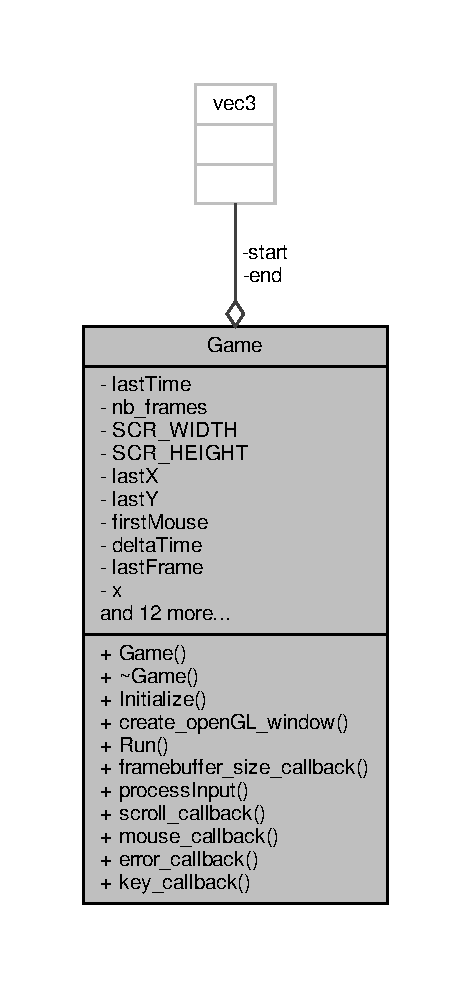
\includegraphics[width=226pt]{classGame__coll__graph}
\end{center}
\end{figure}
\subsection*{Public Member Functions}
\begin{DoxyCompactItemize}
\item 
\hyperlink{classGame_ad59df6562a58a614fda24622d3715b65}{Game} ()
\item 
\hyperlink{classGame_ae3d112ca6e0e55150d2fdbc704474530}{$\sim$\+Game} ()
\item 
void \hyperlink{classGame_adc01a7fae5261c95f7e6b41024e6c533}{Initialize} ()
\item 
G\+L\+F\+Wwindow $\ast$ \hyperlink{classGame_ad25806b818108918a7e5fc5bd71f5de3}{create\+\_\+open\+G\+L\+\_\+window} (int opengl\+\_\+major\+\_\+ver, int opengl\+\_\+minor\+\_\+ver, const char $\ast$win\+\_\+title, int screen\+\_\+width, int screen\+\_\+height)
\item 
void \hyperlink{classGame_a96341ca5b54d90adc3ecb3bf0bcd2312}{Run} ()
\item 
void \hyperlink{classGame_add1087a248a7e136debe003af25f9fa2}{framebuffer\+\_\+size\+\_\+callback} (G\+L\+F\+Wwindow $\ast$window, int width, int height)
\item 
void \hyperlink{classGame_a600b6bf8efd1874f5b5bdb8fdc48e549}{process\+Input} (G\+L\+F\+Wwindow $\ast$window)
\item 
void \hyperlink{classGame_ac3931568d19483386124d89aa0e2a762}{scroll\+\_\+callback} (G\+L\+F\+Wwindow $\ast$window, double xoffset, double yoffset)
\item 
void \hyperlink{classGame_ade7c4fb6814172307baa622f1b4bb566}{mouse\+\_\+callback} (G\+L\+F\+Wwindow $\ast$window, double xpos, double ypos)
\item 
void \hyperlink{classGame_a78d191af16100cc28477474bc0b1e2de}{error\+\_\+callback} (int error, const char $\ast$description)
\end{DoxyCompactItemize}
\subsection*{Static Public Member Functions}
\begin{DoxyCompactItemize}
\item 
static void \hyperlink{classGame_a1622ae34c02e33376dabde5294c9a8e8}{key\+\_\+callback} (G\+L\+F\+Wwindow $\ast$window, int key, int scancode, int action, int mods)
\end{DoxyCompactItemize}
\subsection*{Private Attributes}
\begin{DoxyCompactItemize}
\item 
double \hyperlink{classGame_ace2a5d0114bae5d7aed5019fb7594a74}{last\+Time} = glfw\+Get\+Time()
\item 
int \hyperlink{classGame_a63d5638d248bf98c40198a993acb7116}{nb\+\_\+frames} = 0
\item 
const unsigned int \hyperlink{classGame_ad2b1545413788030fd7e6188997f6f2e}{S\+C\+R\+\_\+\+W\+I\+D\+TH} = 1366
\item 
const unsigned int \hyperlink{classGame_a2c6e67480b144efbf5658a383dc59be6}{S\+C\+R\+\_\+\+H\+E\+I\+G\+HT} = 768
\item 
float \hyperlink{classGame_a842246f215e74d4bddcf3240023e9a69}{lastX} = \hyperlink{classGame_ad2b1545413788030fd7e6188997f6f2e}{S\+C\+R\+\_\+\+W\+I\+D\+TH} / 2.\+0f
\item 
float \hyperlink{classGame_a3d6e621544e978b995d29c23cce7b6ea}{lastY} = \hyperlink{classGame_a2c6e67480b144efbf5658a383dc59be6}{S\+C\+R\+\_\+\+H\+E\+I\+G\+HT} / 2.\+0f
\item 
bool \hyperlink{classGame_a30f99ca78c46117cea01501ef90fadd2}{first\+Mouse} = true
\item 
float \hyperlink{classGame_ad918e31c1644966465f822d912585f16}{delta\+Time} = 0.\+0f
\item 
float \hyperlink{classGame_a4001497330fe92f315d40cb1de2961ee}{last\+Frame} = 0.\+0f
\item 
float \hyperlink{classGame_aaf300d683d6896112e2e901b1024b172}{x}
\item 
float \hyperlink{classGame_a221bbe2ebb32e5ead7d84c6ed08bcbde}{y}
\item 
float \hyperlink{classGame_aafae5c26f5ffa6304824b102ddfedbc8}{r}
\item 
glm\+::vec3 \hyperlink{classGame_a3340408b0b220ba2fa7c21cc024be4ce}{start}
\item 
glm\+::vec3 \hyperlink{classGame_a241457bcabfa070bd4371f7cc20d4ed6}{end}
\item 
float \hyperlink{classGame_afef07f52dd1878b9d0b8aa1b30dbbad8}{x\+\_\+cam}
\item 
float \hyperlink{classGame_a40506d4bac4f3054bbc0ec46963d1405}{y\+\_\+cam}
\item 
float \hyperlink{classGame_a53313ed59bd68bd173dc09b91e982924}{z\+\_\+cam}
\item 
float \hyperlink{classGame_acced6cb4b6acb164ab77f5da29d20467}{r\+\_\+cam}
\item 
glm\+::vec2 \hyperlink{classGame_a84e44c43ed2393f78eb7d1db35af59aa}{z\+\_\+scale}
\item 
\hyperlink{game_8h_a513c9dd465a0df41dbb4daf40cc717c2}{Game\+Data\+Ref} \hyperlink{classGame_a8b54ceb7347e41f1e152c23bc91b618b}{\+\_\+data} = std\+::make\+\_\+shared$<$\hyperlink{structGameData}{Game\+Data}$>$()
\item 
bool \hyperlink{classGame_a03761c5c7c4b941cf1ce77e9867d9dfc}{main\+\_\+menu} = false
\item 
bool \hyperlink{classGame_a9eb1ade97d4575d24c23e480f2fa75fa}{splash} = false
\item 
bool \hyperlink{classGame_ae7f4287e9ee1d3b544679af31fb6da4f}{play} = false
\item 
bool \hyperlink{classGame_ae910a33b0b8246d3ece3d29503d98af7}{game\+\_\+over} = false
\end{DoxyCompactItemize}


\subsection{Constructor \& Destructor Documentation}
\mbox{\Hypertarget{classGame_ad59df6562a58a614fda24622d3715b65}\label{classGame_ad59df6562a58a614fda24622d3715b65}} 
\index{Game@{Game}!Game@{Game}}
\index{Game@{Game}!Game@{Game}}
\subsubsection{\texorpdfstring{Game()}{Game()}}
{\footnotesize\ttfamily Game\+::\+Game (\begin{DoxyParamCaption}{ }\end{DoxyParamCaption})}

\mbox{\Hypertarget{classGame_ae3d112ca6e0e55150d2fdbc704474530}\label{classGame_ae3d112ca6e0e55150d2fdbc704474530}} 
\index{Game@{Game}!````~Game@{$\sim$\+Game}}
\index{````~Game@{$\sim$\+Game}!Game@{Game}}
\subsubsection{\texorpdfstring{$\sim$\+Game()}{~Game()}}
{\footnotesize\ttfamily Game\+::$\sim$\+Game (\begin{DoxyParamCaption}{ }\end{DoxyParamCaption})}



\subsection{Member Function Documentation}
\mbox{\Hypertarget{classGame_ad25806b818108918a7e5fc5bd71f5de3}\label{classGame_ad25806b818108918a7e5fc5bd71f5de3}} 
\index{Game@{Game}!create\+\_\+open\+G\+L\+\_\+window@{create\+\_\+open\+G\+L\+\_\+window}}
\index{create\+\_\+open\+G\+L\+\_\+window@{create\+\_\+open\+G\+L\+\_\+window}!Game@{Game}}
\subsubsection{\texorpdfstring{create\+\_\+open\+G\+L\+\_\+window()}{create\_openGL\_window()}}
{\footnotesize\ttfamily G\+L\+F\+Wwindow $\ast$ Game\+::create\+\_\+open\+G\+L\+\_\+window (\begin{DoxyParamCaption}\item[{int}]{opengl\+\_\+major\+\_\+ver,  }\item[{int}]{opengl\+\_\+minor\+\_\+ver,  }\item[{const char $\ast$}]{win\+\_\+title,  }\item[{int}]{screen\+\_\+width,  }\item[{int}]{screen\+\_\+height }\end{DoxyParamCaption})}

\mbox{\Hypertarget{classGame_a78d191af16100cc28477474bc0b1e2de}\label{classGame_a78d191af16100cc28477474bc0b1e2de}} 
\index{Game@{Game}!error\+\_\+callback@{error\+\_\+callback}}
\index{error\+\_\+callback@{error\+\_\+callback}!Game@{Game}}
\subsubsection{\texorpdfstring{error\+\_\+callback()}{error\_callback()}}
{\footnotesize\ttfamily void Game\+::error\+\_\+callback (\begin{DoxyParamCaption}\item[{int}]{error,  }\item[{const char $\ast$}]{description }\end{DoxyParamCaption})}

\mbox{\Hypertarget{classGame_add1087a248a7e136debe003af25f9fa2}\label{classGame_add1087a248a7e136debe003af25f9fa2}} 
\index{Game@{Game}!framebuffer\+\_\+size\+\_\+callback@{framebuffer\+\_\+size\+\_\+callback}}
\index{framebuffer\+\_\+size\+\_\+callback@{framebuffer\+\_\+size\+\_\+callback}!Game@{Game}}
\subsubsection{\texorpdfstring{framebuffer\+\_\+size\+\_\+callback()}{framebuffer\_size\_callback()}}
{\footnotesize\ttfamily void Game\+::framebuffer\+\_\+size\+\_\+callback (\begin{DoxyParamCaption}\item[{G\+L\+F\+Wwindow $\ast$}]{window,  }\item[{int}]{width,  }\item[{int}]{height }\end{DoxyParamCaption})}

\mbox{\Hypertarget{classGame_adc01a7fae5261c95f7e6b41024e6c533}\label{classGame_adc01a7fae5261c95f7e6b41024e6c533}} 
\index{Game@{Game}!Initialize@{Initialize}}
\index{Initialize@{Initialize}!Game@{Game}}
\subsubsection{\texorpdfstring{Initialize()}{Initialize()}}
{\footnotesize\ttfamily void Game\+::\+Initialize (\begin{DoxyParamCaption}{ }\end{DoxyParamCaption})}

\mbox{\Hypertarget{classGame_a1622ae34c02e33376dabde5294c9a8e8}\label{classGame_a1622ae34c02e33376dabde5294c9a8e8}} 
\index{Game@{Game}!key\+\_\+callback@{key\+\_\+callback}}
\index{key\+\_\+callback@{key\+\_\+callback}!Game@{Game}}
\subsubsection{\texorpdfstring{key\+\_\+callback()}{key\_callback()}}
{\footnotesize\ttfamily static void Game\+::key\+\_\+callback (\begin{DoxyParamCaption}\item[{G\+L\+F\+Wwindow $\ast$}]{window,  }\item[{int}]{key,  }\item[{int}]{scancode,  }\item[{int}]{action,  }\item[{int}]{mods }\end{DoxyParamCaption})\hspace{0.3cm}{\ttfamily [static]}}

\mbox{\Hypertarget{classGame_ade7c4fb6814172307baa622f1b4bb566}\label{classGame_ade7c4fb6814172307baa622f1b4bb566}} 
\index{Game@{Game}!mouse\+\_\+callback@{mouse\+\_\+callback}}
\index{mouse\+\_\+callback@{mouse\+\_\+callback}!Game@{Game}}
\subsubsection{\texorpdfstring{mouse\+\_\+callback()}{mouse\_callback()}}
{\footnotesize\ttfamily void Game\+::mouse\+\_\+callback (\begin{DoxyParamCaption}\item[{G\+L\+F\+Wwindow $\ast$}]{window,  }\item[{double}]{xpos,  }\item[{double}]{ypos }\end{DoxyParamCaption})}

\mbox{\Hypertarget{classGame_a600b6bf8efd1874f5b5bdb8fdc48e549}\label{classGame_a600b6bf8efd1874f5b5bdb8fdc48e549}} 
\index{Game@{Game}!process\+Input@{process\+Input}}
\index{process\+Input@{process\+Input}!Game@{Game}}
\subsubsection{\texorpdfstring{process\+Input()}{processInput()}}
{\footnotesize\ttfamily void Game\+::process\+Input (\begin{DoxyParamCaption}\item[{G\+L\+F\+Wwindow $\ast$}]{window }\end{DoxyParamCaption})}

\mbox{\Hypertarget{classGame_a96341ca5b54d90adc3ecb3bf0bcd2312}\label{classGame_a96341ca5b54d90adc3ecb3bf0bcd2312}} 
\index{Game@{Game}!Run@{Run}}
\index{Run@{Run}!Game@{Game}}
\subsubsection{\texorpdfstring{Run()}{Run()}}
{\footnotesize\ttfamily void Game\+::\+Run (\begin{DoxyParamCaption}{ }\end{DoxyParamCaption})}

\mbox{\Hypertarget{classGame_ac3931568d19483386124d89aa0e2a762}\label{classGame_ac3931568d19483386124d89aa0e2a762}} 
\index{Game@{Game}!scroll\+\_\+callback@{scroll\+\_\+callback}}
\index{scroll\+\_\+callback@{scroll\+\_\+callback}!Game@{Game}}
\subsubsection{\texorpdfstring{scroll\+\_\+callback()}{scroll\_callback()}}
{\footnotesize\ttfamily void Game\+::scroll\+\_\+callback (\begin{DoxyParamCaption}\item[{G\+L\+F\+Wwindow $\ast$}]{window,  }\item[{double}]{xoffset,  }\item[{double}]{yoffset }\end{DoxyParamCaption})}



\subsection{Member Data Documentation}
\mbox{\Hypertarget{classGame_a8b54ceb7347e41f1e152c23bc91b618b}\label{classGame_a8b54ceb7347e41f1e152c23bc91b618b}} 
\index{Game@{Game}!\+\_\+data@{\+\_\+data}}
\index{\+\_\+data@{\+\_\+data}!Game@{Game}}
\subsubsection{\texorpdfstring{\+\_\+data}{\_data}}
{\footnotesize\ttfamily \hyperlink{game_8h_a513c9dd465a0df41dbb4daf40cc717c2}{Game\+Data\+Ref} Game\+::\+\_\+data = std\+::make\+\_\+shared$<$\hyperlink{structGameData}{Game\+Data}$>$()\hspace{0.3cm}{\ttfamily [private]}}

\mbox{\Hypertarget{classGame_ad918e31c1644966465f822d912585f16}\label{classGame_ad918e31c1644966465f822d912585f16}} 
\index{Game@{Game}!delta\+Time@{delta\+Time}}
\index{delta\+Time@{delta\+Time}!Game@{Game}}
\subsubsection{\texorpdfstring{delta\+Time}{deltaTime}}
{\footnotesize\ttfamily float Game\+::delta\+Time = 0.\+0f\hspace{0.3cm}{\ttfamily [private]}}

\mbox{\Hypertarget{classGame_a241457bcabfa070bd4371f7cc20d4ed6}\label{classGame_a241457bcabfa070bd4371f7cc20d4ed6}} 
\index{Game@{Game}!end@{end}}
\index{end@{end}!Game@{Game}}
\subsubsection{\texorpdfstring{end}{end}}
{\footnotesize\ttfamily glm\+::vec3 Game\+::end\hspace{0.3cm}{\ttfamily [private]}}

\mbox{\Hypertarget{classGame_a30f99ca78c46117cea01501ef90fadd2}\label{classGame_a30f99ca78c46117cea01501ef90fadd2}} 
\index{Game@{Game}!first\+Mouse@{first\+Mouse}}
\index{first\+Mouse@{first\+Mouse}!Game@{Game}}
\subsubsection{\texorpdfstring{first\+Mouse}{firstMouse}}
{\footnotesize\ttfamily bool Game\+::first\+Mouse = true\hspace{0.3cm}{\ttfamily [private]}}

\mbox{\Hypertarget{classGame_ae910a33b0b8246d3ece3d29503d98af7}\label{classGame_ae910a33b0b8246d3ece3d29503d98af7}} 
\index{Game@{Game}!game\+\_\+over@{game\+\_\+over}}
\index{game\+\_\+over@{game\+\_\+over}!Game@{Game}}
\subsubsection{\texorpdfstring{game\+\_\+over}{game\_over}}
{\footnotesize\ttfamily bool Game\+::game\+\_\+over = false\hspace{0.3cm}{\ttfamily [private]}}

\mbox{\Hypertarget{classGame_a4001497330fe92f315d40cb1de2961ee}\label{classGame_a4001497330fe92f315d40cb1de2961ee}} 
\index{Game@{Game}!last\+Frame@{last\+Frame}}
\index{last\+Frame@{last\+Frame}!Game@{Game}}
\subsubsection{\texorpdfstring{last\+Frame}{lastFrame}}
{\footnotesize\ttfamily float Game\+::last\+Frame = 0.\+0f\hspace{0.3cm}{\ttfamily [private]}}

\mbox{\Hypertarget{classGame_ace2a5d0114bae5d7aed5019fb7594a74}\label{classGame_ace2a5d0114bae5d7aed5019fb7594a74}} 
\index{Game@{Game}!last\+Time@{last\+Time}}
\index{last\+Time@{last\+Time}!Game@{Game}}
\subsubsection{\texorpdfstring{last\+Time}{lastTime}}
{\footnotesize\ttfamily double Game\+::last\+Time = glfw\+Get\+Time()\hspace{0.3cm}{\ttfamily [private]}}

\mbox{\Hypertarget{classGame_a842246f215e74d4bddcf3240023e9a69}\label{classGame_a842246f215e74d4bddcf3240023e9a69}} 
\index{Game@{Game}!lastX@{lastX}}
\index{lastX@{lastX}!Game@{Game}}
\subsubsection{\texorpdfstring{lastX}{lastX}}
{\footnotesize\ttfamily float Game\+::lastX = \hyperlink{classGame_ad2b1545413788030fd7e6188997f6f2e}{S\+C\+R\+\_\+\+W\+I\+D\+TH} / 2.\+0f\hspace{0.3cm}{\ttfamily [private]}}

\mbox{\Hypertarget{classGame_a3d6e621544e978b995d29c23cce7b6ea}\label{classGame_a3d6e621544e978b995d29c23cce7b6ea}} 
\index{Game@{Game}!lastY@{lastY}}
\index{lastY@{lastY}!Game@{Game}}
\subsubsection{\texorpdfstring{lastY}{lastY}}
{\footnotesize\ttfamily float Game\+::lastY = \hyperlink{classGame_a2c6e67480b144efbf5658a383dc59be6}{S\+C\+R\+\_\+\+H\+E\+I\+G\+HT} / 2.\+0f\hspace{0.3cm}{\ttfamily [private]}}

\mbox{\Hypertarget{classGame_a03761c5c7c4b941cf1ce77e9867d9dfc}\label{classGame_a03761c5c7c4b941cf1ce77e9867d9dfc}} 
\index{Game@{Game}!main\+\_\+menu@{main\+\_\+menu}}
\index{main\+\_\+menu@{main\+\_\+menu}!Game@{Game}}
\subsubsection{\texorpdfstring{main\+\_\+menu}{main\_menu}}
{\footnotesize\ttfamily bool Game\+::main\+\_\+menu = false\hspace{0.3cm}{\ttfamily [private]}}

\mbox{\Hypertarget{classGame_a63d5638d248bf98c40198a993acb7116}\label{classGame_a63d5638d248bf98c40198a993acb7116}} 
\index{Game@{Game}!nb\+\_\+frames@{nb\+\_\+frames}}
\index{nb\+\_\+frames@{nb\+\_\+frames}!Game@{Game}}
\subsubsection{\texorpdfstring{nb\+\_\+frames}{nb\_frames}}
{\footnotesize\ttfamily int Game\+::nb\+\_\+frames = 0\hspace{0.3cm}{\ttfamily [private]}}

\mbox{\Hypertarget{classGame_ae7f4287e9ee1d3b544679af31fb6da4f}\label{classGame_ae7f4287e9ee1d3b544679af31fb6da4f}} 
\index{Game@{Game}!play@{play}}
\index{play@{play}!Game@{Game}}
\subsubsection{\texorpdfstring{play}{play}}
{\footnotesize\ttfamily bool Game\+::play = false\hspace{0.3cm}{\ttfamily [private]}}

\mbox{\Hypertarget{classGame_aafae5c26f5ffa6304824b102ddfedbc8}\label{classGame_aafae5c26f5ffa6304824b102ddfedbc8}} 
\index{Game@{Game}!r@{r}}
\index{r@{r}!Game@{Game}}
\subsubsection{\texorpdfstring{r}{r}}
{\footnotesize\ttfamily float Game\+::r\hspace{0.3cm}{\ttfamily [private]}}

\mbox{\Hypertarget{classGame_acced6cb4b6acb164ab77f5da29d20467}\label{classGame_acced6cb4b6acb164ab77f5da29d20467}} 
\index{Game@{Game}!r\+\_\+cam@{r\+\_\+cam}}
\index{r\+\_\+cam@{r\+\_\+cam}!Game@{Game}}
\subsubsection{\texorpdfstring{r\+\_\+cam}{r\_cam}}
{\footnotesize\ttfamily float Game\+::r\+\_\+cam\hspace{0.3cm}{\ttfamily [private]}}

\mbox{\Hypertarget{classGame_a2c6e67480b144efbf5658a383dc59be6}\label{classGame_a2c6e67480b144efbf5658a383dc59be6}} 
\index{Game@{Game}!S\+C\+R\+\_\+\+H\+E\+I\+G\+HT@{S\+C\+R\+\_\+\+H\+E\+I\+G\+HT}}
\index{S\+C\+R\+\_\+\+H\+E\+I\+G\+HT@{S\+C\+R\+\_\+\+H\+E\+I\+G\+HT}!Game@{Game}}
\subsubsection{\texorpdfstring{S\+C\+R\+\_\+\+H\+E\+I\+G\+HT}{SCR\_HEIGHT}}
{\footnotesize\ttfamily const unsigned int Game\+::\+S\+C\+R\+\_\+\+H\+E\+I\+G\+HT = 768\hspace{0.3cm}{\ttfamily [private]}}

\mbox{\Hypertarget{classGame_ad2b1545413788030fd7e6188997f6f2e}\label{classGame_ad2b1545413788030fd7e6188997f6f2e}} 
\index{Game@{Game}!S\+C\+R\+\_\+\+W\+I\+D\+TH@{S\+C\+R\+\_\+\+W\+I\+D\+TH}}
\index{S\+C\+R\+\_\+\+W\+I\+D\+TH@{S\+C\+R\+\_\+\+W\+I\+D\+TH}!Game@{Game}}
\subsubsection{\texorpdfstring{S\+C\+R\+\_\+\+W\+I\+D\+TH}{SCR\_WIDTH}}
{\footnotesize\ttfamily const unsigned int Game\+::\+S\+C\+R\+\_\+\+W\+I\+D\+TH = 1366\hspace{0.3cm}{\ttfamily [private]}}

\mbox{\Hypertarget{classGame_a9eb1ade97d4575d24c23e480f2fa75fa}\label{classGame_a9eb1ade97d4575d24c23e480f2fa75fa}} 
\index{Game@{Game}!splash@{splash}}
\index{splash@{splash}!Game@{Game}}
\subsubsection{\texorpdfstring{splash}{splash}}
{\footnotesize\ttfamily bool Game\+::splash = false\hspace{0.3cm}{\ttfamily [private]}}

\mbox{\Hypertarget{classGame_a3340408b0b220ba2fa7c21cc024be4ce}\label{classGame_a3340408b0b220ba2fa7c21cc024be4ce}} 
\index{Game@{Game}!start@{start}}
\index{start@{start}!Game@{Game}}
\subsubsection{\texorpdfstring{start}{start}}
{\footnotesize\ttfamily glm\+::vec3 Game\+::start\hspace{0.3cm}{\ttfamily [private]}}

\mbox{\Hypertarget{classGame_aaf300d683d6896112e2e901b1024b172}\label{classGame_aaf300d683d6896112e2e901b1024b172}} 
\index{Game@{Game}!x@{x}}
\index{x@{x}!Game@{Game}}
\subsubsection{\texorpdfstring{x}{x}}
{\footnotesize\ttfamily float Game\+::x\hspace{0.3cm}{\ttfamily [private]}}

\mbox{\Hypertarget{classGame_afef07f52dd1878b9d0b8aa1b30dbbad8}\label{classGame_afef07f52dd1878b9d0b8aa1b30dbbad8}} 
\index{Game@{Game}!x\+\_\+cam@{x\+\_\+cam}}
\index{x\+\_\+cam@{x\+\_\+cam}!Game@{Game}}
\subsubsection{\texorpdfstring{x\+\_\+cam}{x\_cam}}
{\footnotesize\ttfamily float Game\+::x\+\_\+cam\hspace{0.3cm}{\ttfamily [private]}}

\mbox{\Hypertarget{classGame_a221bbe2ebb32e5ead7d84c6ed08bcbde}\label{classGame_a221bbe2ebb32e5ead7d84c6ed08bcbde}} 
\index{Game@{Game}!y@{y}}
\index{y@{y}!Game@{Game}}
\subsubsection{\texorpdfstring{y}{y}}
{\footnotesize\ttfamily float Game\+::y\hspace{0.3cm}{\ttfamily [private]}}

\mbox{\Hypertarget{classGame_a40506d4bac4f3054bbc0ec46963d1405}\label{classGame_a40506d4bac4f3054bbc0ec46963d1405}} 
\index{Game@{Game}!y\+\_\+cam@{y\+\_\+cam}}
\index{y\+\_\+cam@{y\+\_\+cam}!Game@{Game}}
\subsubsection{\texorpdfstring{y\+\_\+cam}{y\_cam}}
{\footnotesize\ttfamily float Game\+::y\+\_\+cam\hspace{0.3cm}{\ttfamily [private]}}

\mbox{\Hypertarget{classGame_a53313ed59bd68bd173dc09b91e982924}\label{classGame_a53313ed59bd68bd173dc09b91e982924}} 
\index{Game@{Game}!z\+\_\+cam@{z\+\_\+cam}}
\index{z\+\_\+cam@{z\+\_\+cam}!Game@{Game}}
\subsubsection{\texorpdfstring{z\+\_\+cam}{z\_cam}}
{\footnotesize\ttfamily float Game\+::z\+\_\+cam\hspace{0.3cm}{\ttfamily [private]}}

\mbox{\Hypertarget{classGame_a84e44c43ed2393f78eb7d1db35af59aa}\label{classGame_a84e44c43ed2393f78eb7d1db35af59aa}} 
\index{Game@{Game}!z\+\_\+scale@{z\+\_\+scale}}
\index{z\+\_\+scale@{z\+\_\+scale}!Game@{Game}}
\subsubsection{\texorpdfstring{z\+\_\+scale}{z\_scale}}
{\footnotesize\ttfamily glm\+::vec2 Game\+::z\+\_\+scale\hspace{0.3cm}{\ttfamily [private]}}



The documentation for this class was generated from the following files\+:\begin{DoxyCompactItemize}
\item 
/mnt/hdd/\+C0de/smart\+\_\+engine/include/\hyperlink{game_8h}{game.\+h}\item 
/mnt/hdd/\+C0de/smart\+\_\+engine/src/\hyperlink{game_8cpp}{game.\+cpp}\end{DoxyCompactItemize}

\hypertarget{classgame__text}{}\section{game\+\_\+text Class Reference}
\label{classgame__text}\index{game\+\_\+text@{game\+\_\+text}}


{\ttfamily \#include $<$game\+\_\+text.\+h$>$}



Collaboration diagram for game\+\_\+text\+:
\nopagebreak
\begin{figure}[H]
\begin{center}
\leavevmode
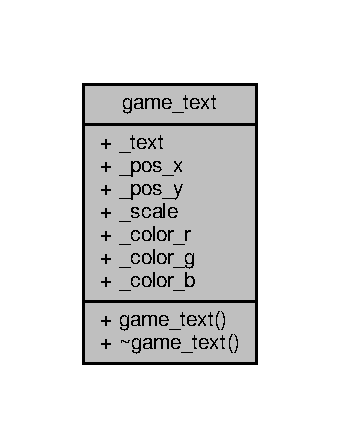
\includegraphics[width=163pt]{classgame__text__coll__graph}
\end{center}
\end{figure}
\subsection*{Public Member Functions}
\begin{DoxyCompactItemize}
\item 
\hyperlink{classgame__text_aeda16b6fac60f1d021bc0ff545771c15}{game\+\_\+text} (std\+::string text, float pos\+\_\+x, float pos\+\_\+y, float scale, float color\+\_\+r, float color\+\_\+g, float color\+\_\+b)
\item 
\hyperlink{classgame__text_a8ac8ab9bd95d07e4482ec2905b5084fc}{$\sim$game\+\_\+text} ()
\end{DoxyCompactItemize}
\subsection*{Public Attributes}
\begin{DoxyCompactItemize}
\item 
std\+::string \hyperlink{classgame__text_ab809f6489478aa8027743e0a624f5de4}{\+\_\+text}
\item 
float \hyperlink{classgame__text_a5209d8b266c524c6f421367d7f6ae075}{\+\_\+pos\+\_\+x}
\item 
float \hyperlink{classgame__text_a5d712db3c22f15d88a6539e63f5135ff}{\+\_\+pos\+\_\+y}
\item 
float \hyperlink{classgame__text_a53ca360266e5df36e8fb809652c45e4c}{\+\_\+scale}
\item 
float \hyperlink{classgame__text_a24db298442718dcf0bfc34be2cadca34}{\+\_\+color\+\_\+r}
\item 
float \hyperlink{classgame__text_aed136aa415fa6edcccdac0f4854b7ae2}{\+\_\+color\+\_\+g}
\item 
float \hyperlink{classgame__text_a7615b072f422ba82917c23e446b065de}{\+\_\+color\+\_\+b}
\end{DoxyCompactItemize}


\subsection{Constructor \& Destructor Documentation}
\mbox{\Hypertarget{classgame__text_aeda16b6fac60f1d021bc0ff545771c15}\label{classgame__text_aeda16b6fac60f1d021bc0ff545771c15}} 
\index{game\+\_\+text@{game\+\_\+text}!game\+\_\+text@{game\+\_\+text}}
\index{game\+\_\+text@{game\+\_\+text}!game\+\_\+text@{game\+\_\+text}}
\subsubsection{\texorpdfstring{game\+\_\+text()}{game\_text()}}
{\footnotesize\ttfamily game\+\_\+text\+::game\+\_\+text (\begin{DoxyParamCaption}\item[{std\+::string}]{text,  }\item[{float}]{pos\+\_\+x,  }\item[{float}]{pos\+\_\+y,  }\item[{float}]{scale,  }\item[{float}]{color\+\_\+r,  }\item[{float}]{color\+\_\+g,  }\item[{float}]{color\+\_\+b }\end{DoxyParamCaption})\hspace{0.3cm}{\ttfamily [inline]}}

\mbox{\Hypertarget{classgame__text_a8ac8ab9bd95d07e4482ec2905b5084fc}\label{classgame__text_a8ac8ab9bd95d07e4482ec2905b5084fc}} 
\index{game\+\_\+text@{game\+\_\+text}!````~game\+\_\+text@{$\sim$game\+\_\+text}}
\index{````~game\+\_\+text@{$\sim$game\+\_\+text}!game\+\_\+text@{game\+\_\+text}}
\subsubsection{\texorpdfstring{$\sim$game\+\_\+text()}{~game\_text()}}
{\footnotesize\ttfamily game\+\_\+text\+::$\sim$game\+\_\+text (\begin{DoxyParamCaption}{ }\end{DoxyParamCaption})\hspace{0.3cm}{\ttfamily [inline]}}



\subsection{Member Data Documentation}
\mbox{\Hypertarget{classgame__text_a7615b072f422ba82917c23e446b065de}\label{classgame__text_a7615b072f422ba82917c23e446b065de}} 
\index{game\+\_\+text@{game\+\_\+text}!\+\_\+color\+\_\+b@{\+\_\+color\+\_\+b}}
\index{\+\_\+color\+\_\+b@{\+\_\+color\+\_\+b}!game\+\_\+text@{game\+\_\+text}}
\subsubsection{\texorpdfstring{\+\_\+color\+\_\+b}{\_color\_b}}
{\footnotesize\ttfamily float game\+\_\+text\+::\+\_\+color\+\_\+b}

\mbox{\Hypertarget{classgame__text_aed136aa415fa6edcccdac0f4854b7ae2}\label{classgame__text_aed136aa415fa6edcccdac0f4854b7ae2}} 
\index{game\+\_\+text@{game\+\_\+text}!\+\_\+color\+\_\+g@{\+\_\+color\+\_\+g}}
\index{\+\_\+color\+\_\+g@{\+\_\+color\+\_\+g}!game\+\_\+text@{game\+\_\+text}}
\subsubsection{\texorpdfstring{\+\_\+color\+\_\+g}{\_color\_g}}
{\footnotesize\ttfamily float game\+\_\+text\+::\+\_\+color\+\_\+g}

\mbox{\Hypertarget{classgame__text_a24db298442718dcf0bfc34be2cadca34}\label{classgame__text_a24db298442718dcf0bfc34be2cadca34}} 
\index{game\+\_\+text@{game\+\_\+text}!\+\_\+color\+\_\+r@{\+\_\+color\+\_\+r}}
\index{\+\_\+color\+\_\+r@{\+\_\+color\+\_\+r}!game\+\_\+text@{game\+\_\+text}}
\subsubsection{\texorpdfstring{\+\_\+color\+\_\+r}{\_color\_r}}
{\footnotesize\ttfamily float game\+\_\+text\+::\+\_\+color\+\_\+r}

\mbox{\Hypertarget{classgame__text_a5209d8b266c524c6f421367d7f6ae075}\label{classgame__text_a5209d8b266c524c6f421367d7f6ae075}} 
\index{game\+\_\+text@{game\+\_\+text}!\+\_\+pos\+\_\+x@{\+\_\+pos\+\_\+x}}
\index{\+\_\+pos\+\_\+x@{\+\_\+pos\+\_\+x}!game\+\_\+text@{game\+\_\+text}}
\subsubsection{\texorpdfstring{\+\_\+pos\+\_\+x}{\_pos\_x}}
{\footnotesize\ttfamily float game\+\_\+text\+::\+\_\+pos\+\_\+x}

\mbox{\Hypertarget{classgame__text_a5d712db3c22f15d88a6539e63f5135ff}\label{classgame__text_a5d712db3c22f15d88a6539e63f5135ff}} 
\index{game\+\_\+text@{game\+\_\+text}!\+\_\+pos\+\_\+y@{\+\_\+pos\+\_\+y}}
\index{\+\_\+pos\+\_\+y@{\+\_\+pos\+\_\+y}!game\+\_\+text@{game\+\_\+text}}
\subsubsection{\texorpdfstring{\+\_\+pos\+\_\+y}{\_pos\_y}}
{\footnotesize\ttfamily float game\+\_\+text\+::\+\_\+pos\+\_\+y}

\mbox{\Hypertarget{classgame__text_a53ca360266e5df36e8fb809652c45e4c}\label{classgame__text_a53ca360266e5df36e8fb809652c45e4c}} 
\index{game\+\_\+text@{game\+\_\+text}!\+\_\+scale@{\+\_\+scale}}
\index{\+\_\+scale@{\+\_\+scale}!game\+\_\+text@{game\+\_\+text}}
\subsubsection{\texorpdfstring{\+\_\+scale}{\_scale}}
{\footnotesize\ttfamily float game\+\_\+text\+::\+\_\+scale}

\mbox{\Hypertarget{classgame__text_ab809f6489478aa8027743e0a624f5de4}\label{classgame__text_ab809f6489478aa8027743e0a624f5de4}} 
\index{game\+\_\+text@{game\+\_\+text}!\+\_\+text@{\+\_\+text}}
\index{\+\_\+text@{\+\_\+text}!game\+\_\+text@{game\+\_\+text}}
\subsubsection{\texorpdfstring{\+\_\+text}{\_text}}
{\footnotesize\ttfamily std\+::string game\+\_\+text\+::\+\_\+text}



The documentation for this class was generated from the following file\+:\begin{DoxyCompactItemize}
\item 
/mnt/hdd/\+C0de/smart\+\_\+engine/include/\hyperlink{game__text_8h}{game\+\_\+text.\+h}\end{DoxyCompactItemize}

\hypertarget{structGameData}{}\section{Game\+Data Struct Reference}
\label{structGameData}\index{Game\+Data@{Game\+Data}}


{\ttfamily \#include $<$game.\+h$>$}



Collaboration diagram for Game\+Data\+:
\nopagebreak
\begin{figure}[H]
\begin{center}
\leavevmode
\includegraphics[width=350pt]{structGameData__coll__graph}
\end{center}
\end{figure}
\subsection*{Public Attributes}
\begin{DoxyCompactItemize}
\item 
G\+L\+F\+Wwindow $\ast$ \hyperlink{structGameData_af9735787501e4c8c1d26787c322cd6dd}{window}
\item 
\hyperlink{classOrthographic__camera}{Orthographic\+\_\+camera} $\ast$ \hyperlink{structGameData_a9e133f6b5e0d19889e94505db479ca69}{o\+\_\+cam}
\item 
\hyperlink{classLoadingGameObjects}{Loading\+Game\+Objects} $\ast$ \hyperlink{structGameData_aaaddd2c1ea34ab4acc9a732879fd92ab}{ld}
\item 
\hyperlink{classEntityManager}{Entity\+Manager} $\ast$ \hyperlink{structGameData_afe20255f5a9a5a93b581cd333ac75853}{manager}
\item 
\hyperlink{classSpriteRenderer}{Sprite\+Renderer} $\ast$ \hyperlink{structGameData_a85da8dd3e426c436097a9f62b34a59f1}{render}
\item 
\hyperlink{classTextRenderer}{Text\+Renderer} $\ast$ \hyperlink{structGameData_a64a9de895cbaf5200a75085c894217f0}{text\+\_\+render}
\item 
\hyperlink{classStateMachine}{State\+Machine} $\ast$ \hyperlink{structGameData_a22d18ba95d18acdf0e77c8c1591c1ec7}{machine}
\end{DoxyCompactItemize}


\subsection{Member Data Documentation}
\mbox{\Hypertarget{structGameData_aaaddd2c1ea34ab4acc9a732879fd92ab}\label{structGameData_aaaddd2c1ea34ab4acc9a732879fd92ab}} 
\index{Game\+Data@{Game\+Data}!ld@{ld}}
\index{ld@{ld}!Game\+Data@{Game\+Data}}
\subsubsection{\texorpdfstring{ld}{ld}}
{\footnotesize\ttfamily \hyperlink{classLoadingGameObjects}{Loading\+Game\+Objects}$\ast$ Game\+Data\+::ld}

\mbox{\Hypertarget{structGameData_a22d18ba95d18acdf0e77c8c1591c1ec7}\label{structGameData_a22d18ba95d18acdf0e77c8c1591c1ec7}} 
\index{Game\+Data@{Game\+Data}!machine@{machine}}
\index{machine@{machine}!Game\+Data@{Game\+Data}}
\subsubsection{\texorpdfstring{machine}{machine}}
{\footnotesize\ttfamily \hyperlink{classStateMachine}{State\+Machine}$\ast$ Game\+Data\+::machine}

\mbox{\Hypertarget{structGameData_afe20255f5a9a5a93b581cd333ac75853}\label{structGameData_afe20255f5a9a5a93b581cd333ac75853}} 
\index{Game\+Data@{Game\+Data}!manager@{manager}}
\index{manager@{manager}!Game\+Data@{Game\+Data}}
\subsubsection{\texorpdfstring{manager}{manager}}
{\footnotesize\ttfamily \hyperlink{classEntityManager}{Entity\+Manager}$\ast$ Game\+Data\+::manager}

\mbox{\Hypertarget{structGameData_a9e133f6b5e0d19889e94505db479ca69}\label{structGameData_a9e133f6b5e0d19889e94505db479ca69}} 
\index{Game\+Data@{Game\+Data}!o\+\_\+cam@{o\+\_\+cam}}
\index{o\+\_\+cam@{o\+\_\+cam}!Game\+Data@{Game\+Data}}
\subsubsection{\texorpdfstring{o\+\_\+cam}{o\_cam}}
{\footnotesize\ttfamily \hyperlink{classOrthographic__camera}{Orthographic\+\_\+camera}$\ast$ Game\+Data\+::o\+\_\+cam}

\mbox{\Hypertarget{structGameData_a85da8dd3e426c436097a9f62b34a59f1}\label{structGameData_a85da8dd3e426c436097a9f62b34a59f1}} 
\index{Game\+Data@{Game\+Data}!render@{render}}
\index{render@{render}!Game\+Data@{Game\+Data}}
\subsubsection{\texorpdfstring{render}{render}}
{\footnotesize\ttfamily \hyperlink{classSpriteRenderer}{Sprite\+Renderer}$\ast$ Game\+Data\+::render}

\mbox{\Hypertarget{structGameData_a64a9de895cbaf5200a75085c894217f0}\label{structGameData_a64a9de895cbaf5200a75085c894217f0}} 
\index{Game\+Data@{Game\+Data}!text\+\_\+render@{text\+\_\+render}}
\index{text\+\_\+render@{text\+\_\+render}!Game\+Data@{Game\+Data}}
\subsubsection{\texorpdfstring{text\+\_\+render}{text\_render}}
{\footnotesize\ttfamily \hyperlink{classTextRenderer}{Text\+Renderer}$\ast$ Game\+Data\+::text\+\_\+render}

\mbox{\Hypertarget{structGameData_af9735787501e4c8c1d26787c322cd6dd}\label{structGameData_af9735787501e4c8c1d26787c322cd6dd}} 
\index{Game\+Data@{Game\+Data}!window@{window}}
\index{window@{window}!Game\+Data@{Game\+Data}}
\subsubsection{\texorpdfstring{window}{window}}
{\footnotesize\ttfamily G\+L\+F\+Wwindow$\ast$ Game\+Data\+::window}



The documentation for this struct was generated from the following file\+:\begin{DoxyCompactItemize}
\item 
/mnt/hdd/\+C0de/smart\+\_\+engine/include/\hyperlink{game_8h}{game.\+h}\end{DoxyCompactItemize}

\hypertarget{classGameOverState}{}\section{Game\+Over\+State Class Reference}
\label{classGameOverState}\index{Game\+Over\+State@{Game\+Over\+State}}


{\ttfamily \#include $<$game\+\_\+over\+\_\+state.\+h$>$}



Inheritance diagram for Game\+Over\+State\+:
\nopagebreak
\begin{figure}[H]
\begin{center}
\leavevmode
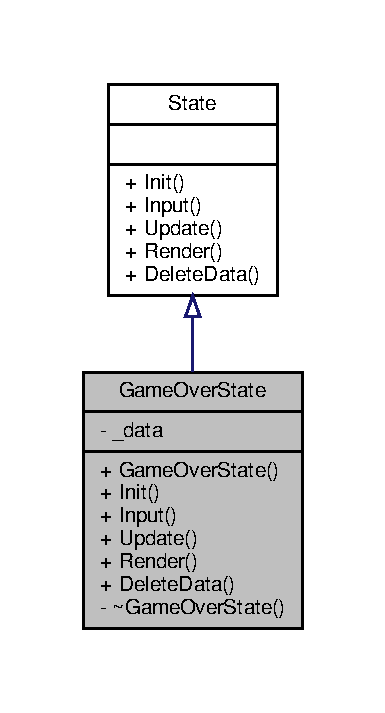
\includegraphics[width=185pt]{classGameOverState__inherit__graph}
\end{center}
\end{figure}


Collaboration diagram for Game\+Over\+State\+:
\nopagebreak
\begin{figure}[H]
\begin{center}
\leavevmode
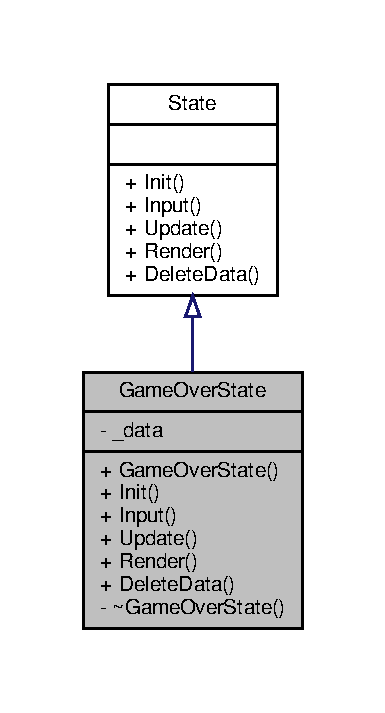
\includegraphics[width=185pt]{classGameOverState__coll__graph}
\end{center}
\end{figure}
\subsection*{Public Member Functions}
\begin{DoxyCompactItemize}
\item 
\hyperlink{classGameOverState_a90dea0468b4719169fd8f5d157e20baf}{Game\+Over\+State} (\hyperlink{game_8h_a513c9dd465a0df41dbb4daf40cc717c2}{Game\+Data\+Ref} data)
\item 
void \hyperlink{classGameOverState_aa3d4f165ff735552f16132e929d369c2}{Init} ()
\item 
void \hyperlink{classGameOverState_adb4be2a5c6292d020999c2da9588ebfc}{Input} (float delta)
\item 
void \hyperlink{classGameOverState_a4dc49d576a9435531f502660119800a9}{Update} (float delta)
\item 
void \hyperlink{classGameOverState_ac9c9ef71b0a12940ac5caa7763f23fdc}{Render} (float delta)
\item 
void \hyperlink{classGameOverState_afb6fa68ff0c5e4f83725de8059c4f7c8}{Delete\+Data} ()
\end{DoxyCompactItemize}
\subsection*{Private Member Functions}
\begin{DoxyCompactItemize}
\item 
\hyperlink{classGameOverState_a6450295ac3a2d64a19bdfe1ad70aacad}{$\sim$\+Game\+Over\+State} ()
\end{DoxyCompactItemize}
\subsection*{Private Attributes}
\begin{DoxyCompactItemize}
\item 
\hyperlink{game_8h_a513c9dd465a0df41dbb4daf40cc717c2}{Game\+Data\+Ref} \hyperlink{classGameOverState_aa3f7f4b44aff376ce1b4aec52fece514}{\+\_\+data}
\end{DoxyCompactItemize}


\subsection{Constructor \& Destructor Documentation}
\mbox{\Hypertarget{classGameOverState_a90dea0468b4719169fd8f5d157e20baf}\label{classGameOverState_a90dea0468b4719169fd8f5d157e20baf}} 
\index{Game\+Over\+State@{Game\+Over\+State}!Game\+Over\+State@{Game\+Over\+State}}
\index{Game\+Over\+State@{Game\+Over\+State}!Game\+Over\+State@{Game\+Over\+State}}
\subsubsection{\texorpdfstring{Game\+Over\+State()}{GameOverState()}}
{\footnotesize\ttfamily Game\+Over\+State\+::\+Game\+Over\+State (\begin{DoxyParamCaption}\item[{\hyperlink{game_8h_a513c9dd465a0df41dbb4daf40cc717c2}{Game\+Data\+Ref}}]{data }\end{DoxyParamCaption})}

\mbox{\Hypertarget{classGameOverState_a6450295ac3a2d64a19bdfe1ad70aacad}\label{classGameOverState_a6450295ac3a2d64a19bdfe1ad70aacad}} 
\index{Game\+Over\+State@{Game\+Over\+State}!````~Game\+Over\+State@{$\sim$\+Game\+Over\+State}}
\index{````~Game\+Over\+State@{$\sim$\+Game\+Over\+State}!Game\+Over\+State@{Game\+Over\+State}}
\subsubsection{\texorpdfstring{$\sim$\+Game\+Over\+State()}{~GameOverState()}}
{\footnotesize\ttfamily Game\+Over\+State\+::$\sim$\+Game\+Over\+State (\begin{DoxyParamCaption}{ }\end{DoxyParamCaption})\hspace{0.3cm}{\ttfamily [private]}}



\subsection{Member Function Documentation}
\mbox{\Hypertarget{classGameOverState_afb6fa68ff0c5e4f83725de8059c4f7c8}\label{classGameOverState_afb6fa68ff0c5e4f83725de8059c4f7c8}} 
\index{Game\+Over\+State@{Game\+Over\+State}!Delete\+Data@{Delete\+Data}}
\index{Delete\+Data@{Delete\+Data}!Game\+Over\+State@{Game\+Over\+State}}
\subsubsection{\texorpdfstring{Delete\+Data()}{DeleteData()}}
{\footnotesize\ttfamily void Game\+Over\+State\+::\+Delete\+Data (\begin{DoxyParamCaption}{ }\end{DoxyParamCaption})\hspace{0.3cm}{\ttfamily [virtual]}}



Implements \hyperlink{classState_ade502eaa386d570e526eb356ffd73fd8}{State}.

\mbox{\Hypertarget{classGameOverState_aa3d4f165ff735552f16132e929d369c2}\label{classGameOverState_aa3d4f165ff735552f16132e929d369c2}} 
\index{Game\+Over\+State@{Game\+Over\+State}!Init@{Init}}
\index{Init@{Init}!Game\+Over\+State@{Game\+Over\+State}}
\subsubsection{\texorpdfstring{Init()}{Init()}}
{\footnotesize\ttfamily void Game\+Over\+State\+::\+Init (\begin{DoxyParamCaption}{ }\end{DoxyParamCaption})\hspace{0.3cm}{\ttfamily [virtual]}}



Implements \hyperlink{classState_a7ab4d8c6aa239a17ed579d89a209b156}{State}.

\mbox{\Hypertarget{classGameOverState_adb4be2a5c6292d020999c2da9588ebfc}\label{classGameOverState_adb4be2a5c6292d020999c2da9588ebfc}} 
\index{Game\+Over\+State@{Game\+Over\+State}!Input@{Input}}
\index{Input@{Input}!Game\+Over\+State@{Game\+Over\+State}}
\subsubsection{\texorpdfstring{Input()}{Input()}}
{\footnotesize\ttfamily void Game\+Over\+State\+::\+Input (\begin{DoxyParamCaption}\item[{float}]{delta }\end{DoxyParamCaption})\hspace{0.3cm}{\ttfamily [virtual]}}



Implements \hyperlink{classState_a1705412877f37a5cc8fc712542756076}{State}.

\mbox{\Hypertarget{classGameOverState_ac9c9ef71b0a12940ac5caa7763f23fdc}\label{classGameOverState_ac9c9ef71b0a12940ac5caa7763f23fdc}} 
\index{Game\+Over\+State@{Game\+Over\+State}!Render@{Render}}
\index{Render@{Render}!Game\+Over\+State@{Game\+Over\+State}}
\subsubsection{\texorpdfstring{Render()}{Render()}}
{\footnotesize\ttfamily void Game\+Over\+State\+::\+Render (\begin{DoxyParamCaption}\item[{float}]{delta }\end{DoxyParamCaption})\hspace{0.3cm}{\ttfamily [virtual]}}



Implements \hyperlink{classState_a0e48dfae1e3090630475812681417c5f}{State}.

\mbox{\Hypertarget{classGameOverState_a4dc49d576a9435531f502660119800a9}\label{classGameOverState_a4dc49d576a9435531f502660119800a9}} 
\index{Game\+Over\+State@{Game\+Over\+State}!Update@{Update}}
\index{Update@{Update}!Game\+Over\+State@{Game\+Over\+State}}
\subsubsection{\texorpdfstring{Update()}{Update()}}
{\footnotesize\ttfamily void Game\+Over\+State\+::\+Update (\begin{DoxyParamCaption}\item[{float}]{delta }\end{DoxyParamCaption})\hspace{0.3cm}{\ttfamily [virtual]}}



Implements \hyperlink{classState_aac0d3fdee1341e168af730b8f31a7bf1}{State}.



\subsection{Member Data Documentation}
\mbox{\Hypertarget{classGameOverState_aa3f7f4b44aff376ce1b4aec52fece514}\label{classGameOverState_aa3f7f4b44aff376ce1b4aec52fece514}} 
\index{Game\+Over\+State@{Game\+Over\+State}!\+\_\+data@{\+\_\+data}}
\index{\+\_\+data@{\+\_\+data}!Game\+Over\+State@{Game\+Over\+State}}
\subsubsection{\texorpdfstring{\+\_\+data}{\_data}}
{\footnotesize\ttfamily \hyperlink{game_8h_a513c9dd465a0df41dbb4daf40cc717c2}{Game\+Data\+Ref} Game\+Over\+State\+::\+\_\+data\hspace{0.3cm}{\ttfamily [private]}}



The documentation for this class was generated from the following files\+:\begin{DoxyCompactItemize}
\item 
/mnt/hdd/\+C0de/smart\+\_\+engine/include/\hyperlink{game__over__state_8h}{game\+\_\+over\+\_\+state.\+h}\item 
/mnt/hdd/\+C0de/smart\+\_\+engine/src/\hyperlink{game__over__state_8cpp}{game\+\_\+over\+\_\+state.\+cpp}\end{DoxyCompactItemize}

\hypertarget{classGamePlayState}{}\section{Game\+Play\+State Class Reference}
\label{classGamePlayState}\index{Game\+Play\+State@{Game\+Play\+State}}


{\ttfamily \#include $<$game\+\_\+play\+\_\+state.\+h$>$}



Inheritance diagram for Game\+Play\+State\+:
\nopagebreak
\begin{figure}[H]
\begin{center}
\leavevmode
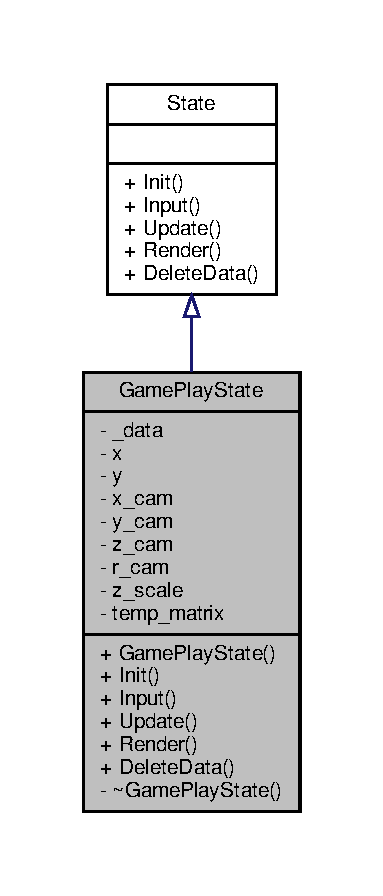
\includegraphics[width=184pt]{classGamePlayState__inherit__graph}
\end{center}
\end{figure}


Collaboration diagram for Game\+Play\+State\+:
\nopagebreak
\begin{figure}[H]
\begin{center}
\leavevmode
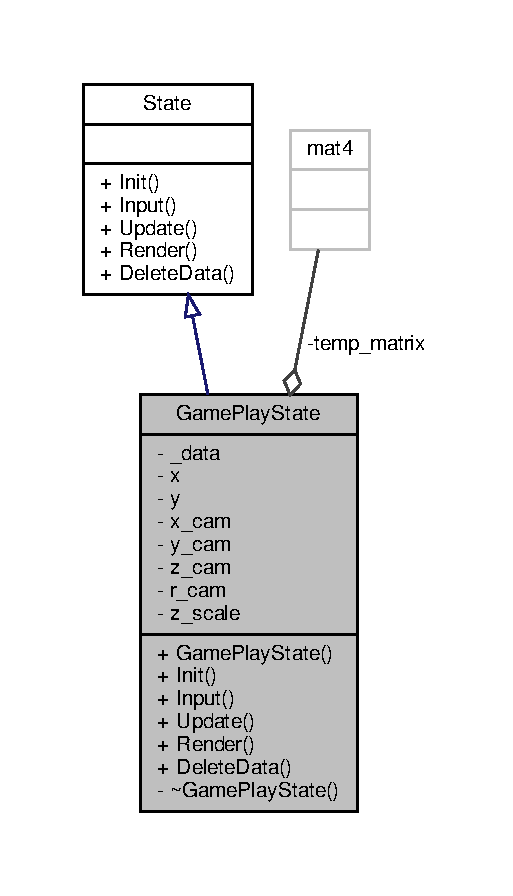
\includegraphics[width=246pt]{classGamePlayState__coll__graph}
\end{center}
\end{figure}
\subsection*{Public Member Functions}
\begin{DoxyCompactItemize}
\item 
\hyperlink{classGamePlayState_a189d187dd3caac0691e1862a89172223}{Game\+Play\+State} (\hyperlink{game_8h_a513c9dd465a0df41dbb4daf40cc717c2}{Game\+Data\+Ref} data)
\item 
void \hyperlink{classGamePlayState_ae13389eea1f83f27d18ba200f107937d}{Init} ()
\item 
void \hyperlink{classGamePlayState_a3bc9231fd11546b5dd13581ed2aa1afa}{Input} (float delta)
\item 
void \hyperlink{classGamePlayState_a19bcc1ff2a83a3aa001010ae35d67b85}{Update} (float delta)
\item 
void \hyperlink{classGamePlayState_a4bd296aa04088a3d8249f569e86f21a7}{Render} (float delta)
\item 
void \hyperlink{classGamePlayState_a8a393249f2deabe0fe8f236b4e58cb17}{Delete\+Data} ()
\end{DoxyCompactItemize}
\subsection*{Private Member Functions}
\begin{DoxyCompactItemize}
\item 
\hyperlink{classGamePlayState_aaa1afd5f6e091e5cb5bda2fa82247d58}{$\sim$\+Game\+Play\+State} ()
\end{DoxyCompactItemize}
\subsection*{Private Attributes}
\begin{DoxyCompactItemize}
\item 
\hyperlink{game_8h_a513c9dd465a0df41dbb4daf40cc717c2}{Game\+Data\+Ref} \hyperlink{classGamePlayState_aab402d0ac13aa45c16e0f89bcfe7e963}{\+\_\+data}
\item 
float \hyperlink{classGamePlayState_a055feaf3b4acaaff53dddc571252c4e4}{x}
\item 
float \hyperlink{classGamePlayState_ae1da324a3664591e663d09a5b17f9007}{y}
\item 
float \hyperlink{classGamePlayState_a1f0c5c88f94177891ec0819628d0aa8c}{x\+\_\+cam}
\item 
float \hyperlink{classGamePlayState_ab69b90dcdbb3375687e6e3641d1654da}{y\+\_\+cam}
\item 
float \hyperlink{classGamePlayState_a3b25b85d41324ec556fe81a75bb1811f}{z\+\_\+cam}
\item 
float \hyperlink{classGamePlayState_a430ff4098f9f58fe0b6ab4fe154a89a0}{r\+\_\+cam}
\item 
glm\+::vec2 \hyperlink{classGamePlayState_a9bdc2e5899e9ca4e266019f646d2ba34}{z\+\_\+scale}
\item 
glm\+::mat4 \hyperlink{classGamePlayState_add3118e821461399143e4f2fd3520966}{temp\+\_\+matrix}
\end{DoxyCompactItemize}


\subsection{Constructor \& Destructor Documentation}
\mbox{\Hypertarget{classGamePlayState_a189d187dd3caac0691e1862a89172223}\label{classGamePlayState_a189d187dd3caac0691e1862a89172223}} 
\index{Game\+Play\+State@{Game\+Play\+State}!Game\+Play\+State@{Game\+Play\+State}}
\index{Game\+Play\+State@{Game\+Play\+State}!Game\+Play\+State@{Game\+Play\+State}}
\subsubsection{\texorpdfstring{Game\+Play\+State()}{GamePlayState()}}
{\footnotesize\ttfamily Game\+Play\+State\+::\+Game\+Play\+State (\begin{DoxyParamCaption}\item[{\hyperlink{game_8h_a513c9dd465a0df41dbb4daf40cc717c2}{Game\+Data\+Ref}}]{data }\end{DoxyParamCaption})}

\mbox{\Hypertarget{classGamePlayState_aaa1afd5f6e091e5cb5bda2fa82247d58}\label{classGamePlayState_aaa1afd5f6e091e5cb5bda2fa82247d58}} 
\index{Game\+Play\+State@{Game\+Play\+State}!````~Game\+Play\+State@{$\sim$\+Game\+Play\+State}}
\index{````~Game\+Play\+State@{$\sim$\+Game\+Play\+State}!Game\+Play\+State@{Game\+Play\+State}}
\subsubsection{\texorpdfstring{$\sim$\+Game\+Play\+State()}{~GamePlayState()}}
{\footnotesize\ttfamily Game\+Play\+State\+::$\sim$\+Game\+Play\+State (\begin{DoxyParamCaption}{ }\end{DoxyParamCaption})\hspace{0.3cm}{\ttfamily [private]}}



\subsection{Member Function Documentation}
\mbox{\Hypertarget{classGamePlayState_a8a393249f2deabe0fe8f236b4e58cb17}\label{classGamePlayState_a8a393249f2deabe0fe8f236b4e58cb17}} 
\index{Game\+Play\+State@{Game\+Play\+State}!Delete\+Data@{Delete\+Data}}
\index{Delete\+Data@{Delete\+Data}!Game\+Play\+State@{Game\+Play\+State}}
\subsubsection{\texorpdfstring{Delete\+Data()}{DeleteData()}}
{\footnotesize\ttfamily void Game\+Play\+State\+::\+Delete\+Data (\begin{DoxyParamCaption}{ }\end{DoxyParamCaption})\hspace{0.3cm}{\ttfamily [virtual]}}



Implements \hyperlink{classState_ade502eaa386d570e526eb356ffd73fd8}{State}.

\mbox{\Hypertarget{classGamePlayState_ae13389eea1f83f27d18ba200f107937d}\label{classGamePlayState_ae13389eea1f83f27d18ba200f107937d}} 
\index{Game\+Play\+State@{Game\+Play\+State}!Init@{Init}}
\index{Init@{Init}!Game\+Play\+State@{Game\+Play\+State}}
\subsubsection{\texorpdfstring{Init()}{Init()}}
{\footnotesize\ttfamily void Game\+Play\+State\+::\+Init (\begin{DoxyParamCaption}{ }\end{DoxyParamCaption})\hspace{0.3cm}{\ttfamily [virtual]}}



Implements \hyperlink{classState_a7ab4d8c6aa239a17ed579d89a209b156}{State}.

\mbox{\Hypertarget{classGamePlayState_a3bc9231fd11546b5dd13581ed2aa1afa}\label{classGamePlayState_a3bc9231fd11546b5dd13581ed2aa1afa}} 
\index{Game\+Play\+State@{Game\+Play\+State}!Input@{Input}}
\index{Input@{Input}!Game\+Play\+State@{Game\+Play\+State}}
\subsubsection{\texorpdfstring{Input()}{Input()}}
{\footnotesize\ttfamily void Game\+Play\+State\+::\+Input (\begin{DoxyParamCaption}\item[{float}]{delta }\end{DoxyParamCaption})\hspace{0.3cm}{\ttfamily [virtual]}}



Implements \hyperlink{classState_a1705412877f37a5cc8fc712542756076}{State}.

\mbox{\Hypertarget{classGamePlayState_a4bd296aa04088a3d8249f569e86f21a7}\label{classGamePlayState_a4bd296aa04088a3d8249f569e86f21a7}} 
\index{Game\+Play\+State@{Game\+Play\+State}!Render@{Render}}
\index{Render@{Render}!Game\+Play\+State@{Game\+Play\+State}}
\subsubsection{\texorpdfstring{Render()}{Render()}}
{\footnotesize\ttfamily void Game\+Play\+State\+::\+Render (\begin{DoxyParamCaption}\item[{float}]{delta }\end{DoxyParamCaption})\hspace{0.3cm}{\ttfamily [virtual]}}



Implements \hyperlink{classState_a0e48dfae1e3090630475812681417c5f}{State}.

\mbox{\Hypertarget{classGamePlayState_a19bcc1ff2a83a3aa001010ae35d67b85}\label{classGamePlayState_a19bcc1ff2a83a3aa001010ae35d67b85}} 
\index{Game\+Play\+State@{Game\+Play\+State}!Update@{Update}}
\index{Update@{Update}!Game\+Play\+State@{Game\+Play\+State}}
\subsubsection{\texorpdfstring{Update()}{Update()}}
{\footnotesize\ttfamily void Game\+Play\+State\+::\+Update (\begin{DoxyParamCaption}\item[{float}]{delta }\end{DoxyParamCaption})\hspace{0.3cm}{\ttfamily [virtual]}}



Implements \hyperlink{classState_aac0d3fdee1341e168af730b8f31a7bf1}{State}.



\subsection{Member Data Documentation}
\mbox{\Hypertarget{classGamePlayState_aab402d0ac13aa45c16e0f89bcfe7e963}\label{classGamePlayState_aab402d0ac13aa45c16e0f89bcfe7e963}} 
\index{Game\+Play\+State@{Game\+Play\+State}!\+\_\+data@{\+\_\+data}}
\index{\+\_\+data@{\+\_\+data}!Game\+Play\+State@{Game\+Play\+State}}
\subsubsection{\texorpdfstring{\+\_\+data}{\_data}}
{\footnotesize\ttfamily \hyperlink{game_8h_a513c9dd465a0df41dbb4daf40cc717c2}{Game\+Data\+Ref} Game\+Play\+State\+::\+\_\+data\hspace{0.3cm}{\ttfamily [private]}}

\mbox{\Hypertarget{classGamePlayState_a430ff4098f9f58fe0b6ab4fe154a89a0}\label{classGamePlayState_a430ff4098f9f58fe0b6ab4fe154a89a0}} 
\index{Game\+Play\+State@{Game\+Play\+State}!r\+\_\+cam@{r\+\_\+cam}}
\index{r\+\_\+cam@{r\+\_\+cam}!Game\+Play\+State@{Game\+Play\+State}}
\subsubsection{\texorpdfstring{r\+\_\+cam}{r\_cam}}
{\footnotesize\ttfamily float Game\+Play\+State\+::r\+\_\+cam\hspace{0.3cm}{\ttfamily [private]}}

\mbox{\Hypertarget{classGamePlayState_add3118e821461399143e4f2fd3520966}\label{classGamePlayState_add3118e821461399143e4f2fd3520966}} 
\index{Game\+Play\+State@{Game\+Play\+State}!temp\+\_\+matrix@{temp\+\_\+matrix}}
\index{temp\+\_\+matrix@{temp\+\_\+matrix}!Game\+Play\+State@{Game\+Play\+State}}
\subsubsection{\texorpdfstring{temp\+\_\+matrix}{temp\_matrix}}
{\footnotesize\ttfamily glm\+::mat4 Game\+Play\+State\+::temp\+\_\+matrix\hspace{0.3cm}{\ttfamily [private]}}

\mbox{\Hypertarget{classGamePlayState_a055feaf3b4acaaff53dddc571252c4e4}\label{classGamePlayState_a055feaf3b4acaaff53dddc571252c4e4}} 
\index{Game\+Play\+State@{Game\+Play\+State}!x@{x}}
\index{x@{x}!Game\+Play\+State@{Game\+Play\+State}}
\subsubsection{\texorpdfstring{x}{x}}
{\footnotesize\ttfamily float Game\+Play\+State\+::x\hspace{0.3cm}{\ttfamily [private]}}

\mbox{\Hypertarget{classGamePlayState_a1f0c5c88f94177891ec0819628d0aa8c}\label{classGamePlayState_a1f0c5c88f94177891ec0819628d0aa8c}} 
\index{Game\+Play\+State@{Game\+Play\+State}!x\+\_\+cam@{x\+\_\+cam}}
\index{x\+\_\+cam@{x\+\_\+cam}!Game\+Play\+State@{Game\+Play\+State}}
\subsubsection{\texorpdfstring{x\+\_\+cam}{x\_cam}}
{\footnotesize\ttfamily float Game\+Play\+State\+::x\+\_\+cam\hspace{0.3cm}{\ttfamily [private]}}

\mbox{\Hypertarget{classGamePlayState_ae1da324a3664591e663d09a5b17f9007}\label{classGamePlayState_ae1da324a3664591e663d09a5b17f9007}} 
\index{Game\+Play\+State@{Game\+Play\+State}!y@{y}}
\index{y@{y}!Game\+Play\+State@{Game\+Play\+State}}
\subsubsection{\texorpdfstring{y}{y}}
{\footnotesize\ttfamily float Game\+Play\+State\+::y\hspace{0.3cm}{\ttfamily [private]}}

\mbox{\Hypertarget{classGamePlayState_ab69b90dcdbb3375687e6e3641d1654da}\label{classGamePlayState_ab69b90dcdbb3375687e6e3641d1654da}} 
\index{Game\+Play\+State@{Game\+Play\+State}!y\+\_\+cam@{y\+\_\+cam}}
\index{y\+\_\+cam@{y\+\_\+cam}!Game\+Play\+State@{Game\+Play\+State}}
\subsubsection{\texorpdfstring{y\+\_\+cam}{y\_cam}}
{\footnotesize\ttfamily float Game\+Play\+State\+::y\+\_\+cam\hspace{0.3cm}{\ttfamily [private]}}

\mbox{\Hypertarget{classGamePlayState_a3b25b85d41324ec556fe81a75bb1811f}\label{classGamePlayState_a3b25b85d41324ec556fe81a75bb1811f}} 
\index{Game\+Play\+State@{Game\+Play\+State}!z\+\_\+cam@{z\+\_\+cam}}
\index{z\+\_\+cam@{z\+\_\+cam}!Game\+Play\+State@{Game\+Play\+State}}
\subsubsection{\texorpdfstring{z\+\_\+cam}{z\_cam}}
{\footnotesize\ttfamily float Game\+Play\+State\+::z\+\_\+cam\hspace{0.3cm}{\ttfamily [private]}}

\mbox{\Hypertarget{classGamePlayState_a9bdc2e5899e9ca4e266019f646d2ba34}\label{classGamePlayState_a9bdc2e5899e9ca4e266019f646d2ba34}} 
\index{Game\+Play\+State@{Game\+Play\+State}!z\+\_\+scale@{z\+\_\+scale}}
\index{z\+\_\+scale@{z\+\_\+scale}!Game\+Play\+State@{Game\+Play\+State}}
\subsubsection{\texorpdfstring{z\+\_\+scale}{z\_scale}}
{\footnotesize\ttfamily glm\+::vec2 Game\+Play\+State\+::z\+\_\+scale\hspace{0.3cm}{\ttfamily [private]}}



The documentation for this class was generated from the following files\+:\begin{DoxyCompactItemize}
\item 
/mnt/hdd/\+C0de/smart\+\_\+engine/include/\hyperlink{game__play__state_8h}{game\+\_\+play\+\_\+state.\+h}\item 
/mnt/hdd/\+C0de/smart\+\_\+engine/src/\hyperlink{game__play__state_8cpp}{game\+\_\+play\+\_\+state.\+cpp}\end{DoxyCompactItemize}

\hypertarget{classLine}{}\section{Line Class Reference}
\label{classLine}\index{Line@{Line}}


Collaboration diagram for Line\+:
\nopagebreak
\begin{figure}[H]
\begin{center}
\leavevmode
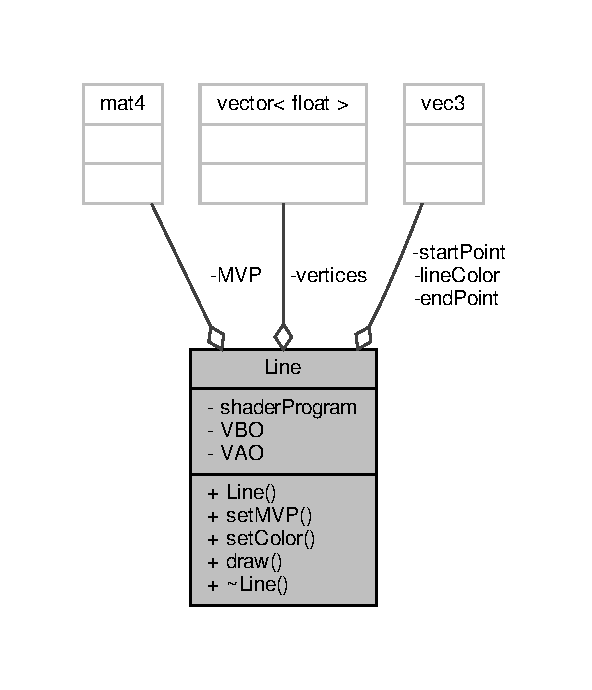
\includegraphics[width=284pt]{classLine__coll__graph}
\end{center}
\end{figure}
\subsection*{Public Member Functions}
\begin{DoxyCompactItemize}
\item 
\hyperlink{classLine_aae4b6f0aa93bf671632a9c932ce81164}{Line} (vec3 start, vec3 end)
\item 
int \hyperlink{classLine_a3ccc376f8f6fadaa88d9e6687a179a45}{set\+M\+VP} (mat4 mvp)
\item 
int \hyperlink{classLine_ac1cf708f780fe795ac17939dd9aa44e2}{set\+Color} (vec3 color)
\item 
int \hyperlink{classLine_ac12e023f79f63cf502683e82c47ba9d8}{draw} ()
\item 
\hyperlink{classLine_aabe85f48d22d92b62257091f48174fac}{$\sim$\+Line} ()
\end{DoxyCompactItemize}
\subsection*{Private Attributes}
\begin{DoxyCompactItemize}
\item 
int \hyperlink{classLine_a878054adb2870a07cd412214302b60d5}{shader\+Program}
\item 
unsigned int \hyperlink{classLine_a24a4150cae9dbaa98d0f21c6be6c7755}{V\+BO}
\item 
unsigned int \hyperlink{classLine_aa17e21db4b9157d666a0c18c18552018}{V\+AO}
\item 
vector$<$ float $>$ \hyperlink{classLine_a161c9dfa204c9758a47b58d9902d5c2c}{vertices}
\item 
vec3 \hyperlink{classLine_a84483386d92f8d092aab79e611095134}{start\+Point}
\item 
vec3 \hyperlink{classLine_aa59cf1049e8a0781bcd410381a1a413d}{end\+Point}
\item 
mat4 \hyperlink{classLine_af3438d68650cd3d26733d4c2043b3c1f}{M\+VP} = mat4(1.\+0)
\item 
vec3 \hyperlink{classLine_a20e21995b7bf5cf61d68e8cf94e42f3d}{line\+Color}
\end{DoxyCompactItemize}


\subsection{Constructor \& Destructor Documentation}
\mbox{\Hypertarget{classLine_aae4b6f0aa93bf671632a9c932ce81164}\label{classLine_aae4b6f0aa93bf671632a9c932ce81164}} 
\index{Line@{Line}!Line@{Line}}
\index{Line@{Line}!Line@{Line}}
\subsubsection{\texorpdfstring{Line()}{Line()}}
{\footnotesize\ttfamily Line\+::\+Line (\begin{DoxyParamCaption}\item[{vec3}]{start,  }\item[{vec3}]{end }\end{DoxyParamCaption})\hspace{0.3cm}{\ttfamily [inline]}}

\mbox{\Hypertarget{classLine_aabe85f48d22d92b62257091f48174fac}\label{classLine_aabe85f48d22d92b62257091f48174fac}} 
\index{Line@{Line}!````~Line@{$\sim$\+Line}}
\index{````~Line@{$\sim$\+Line}!Line@{Line}}
\subsubsection{\texorpdfstring{$\sim$\+Line()}{~Line()}}
{\footnotesize\ttfamily Line\+::$\sim$\+Line (\begin{DoxyParamCaption}{ }\end{DoxyParamCaption})\hspace{0.3cm}{\ttfamily [inline]}}



\subsection{Member Function Documentation}
\mbox{\Hypertarget{classLine_ac12e023f79f63cf502683e82c47ba9d8}\label{classLine_ac12e023f79f63cf502683e82c47ba9d8}} 
\index{Line@{Line}!draw@{draw}}
\index{draw@{draw}!Line@{Line}}
\subsubsection{\texorpdfstring{draw()}{draw()}}
{\footnotesize\ttfamily int Line\+::draw (\begin{DoxyParamCaption}{ }\end{DoxyParamCaption})\hspace{0.3cm}{\ttfamily [inline]}}

\mbox{\Hypertarget{classLine_ac1cf708f780fe795ac17939dd9aa44e2}\label{classLine_ac1cf708f780fe795ac17939dd9aa44e2}} 
\index{Line@{Line}!set\+Color@{set\+Color}}
\index{set\+Color@{set\+Color}!Line@{Line}}
\subsubsection{\texorpdfstring{set\+Color()}{setColor()}}
{\footnotesize\ttfamily int Line\+::set\+Color (\begin{DoxyParamCaption}\item[{vec3}]{color }\end{DoxyParamCaption})\hspace{0.3cm}{\ttfamily [inline]}}

\mbox{\Hypertarget{classLine_a3ccc376f8f6fadaa88d9e6687a179a45}\label{classLine_a3ccc376f8f6fadaa88d9e6687a179a45}} 
\index{Line@{Line}!set\+M\+VP@{set\+M\+VP}}
\index{set\+M\+VP@{set\+M\+VP}!Line@{Line}}
\subsubsection{\texorpdfstring{set\+M\+V\+P()}{setMVP()}}
{\footnotesize\ttfamily int Line\+::set\+M\+VP (\begin{DoxyParamCaption}\item[{mat4}]{mvp }\end{DoxyParamCaption})\hspace{0.3cm}{\ttfamily [inline]}}



\subsection{Member Data Documentation}
\mbox{\Hypertarget{classLine_aa59cf1049e8a0781bcd410381a1a413d}\label{classLine_aa59cf1049e8a0781bcd410381a1a413d}} 
\index{Line@{Line}!end\+Point@{end\+Point}}
\index{end\+Point@{end\+Point}!Line@{Line}}
\subsubsection{\texorpdfstring{end\+Point}{endPoint}}
{\footnotesize\ttfamily vec3 Line\+::end\+Point\hspace{0.3cm}{\ttfamily [private]}}

\mbox{\Hypertarget{classLine_a20e21995b7bf5cf61d68e8cf94e42f3d}\label{classLine_a20e21995b7bf5cf61d68e8cf94e42f3d}} 
\index{Line@{Line}!line\+Color@{line\+Color}}
\index{line\+Color@{line\+Color}!Line@{Line}}
\subsubsection{\texorpdfstring{line\+Color}{lineColor}}
{\footnotesize\ttfamily vec3 Line\+::line\+Color\hspace{0.3cm}{\ttfamily [private]}}

\mbox{\Hypertarget{classLine_af3438d68650cd3d26733d4c2043b3c1f}\label{classLine_af3438d68650cd3d26733d4c2043b3c1f}} 
\index{Line@{Line}!M\+VP@{M\+VP}}
\index{M\+VP@{M\+VP}!Line@{Line}}
\subsubsection{\texorpdfstring{M\+VP}{MVP}}
{\footnotesize\ttfamily mat4 Line\+::\+M\+VP = mat4(1.\+0)\hspace{0.3cm}{\ttfamily [private]}}

\mbox{\Hypertarget{classLine_a878054adb2870a07cd412214302b60d5}\label{classLine_a878054adb2870a07cd412214302b60d5}} 
\index{Line@{Line}!shader\+Program@{shader\+Program}}
\index{shader\+Program@{shader\+Program}!Line@{Line}}
\subsubsection{\texorpdfstring{shader\+Program}{shaderProgram}}
{\footnotesize\ttfamily int Line\+::shader\+Program\hspace{0.3cm}{\ttfamily [private]}}

\mbox{\Hypertarget{classLine_a84483386d92f8d092aab79e611095134}\label{classLine_a84483386d92f8d092aab79e611095134}} 
\index{Line@{Line}!start\+Point@{start\+Point}}
\index{start\+Point@{start\+Point}!Line@{Line}}
\subsubsection{\texorpdfstring{start\+Point}{startPoint}}
{\footnotesize\ttfamily vec3 Line\+::start\+Point\hspace{0.3cm}{\ttfamily [private]}}

\mbox{\Hypertarget{classLine_aa17e21db4b9157d666a0c18c18552018}\label{classLine_aa17e21db4b9157d666a0c18c18552018}} 
\index{Line@{Line}!V\+AO@{V\+AO}}
\index{V\+AO@{V\+AO}!Line@{Line}}
\subsubsection{\texorpdfstring{V\+AO}{VAO}}
{\footnotesize\ttfamily unsigned int Line\+::\+V\+AO\hspace{0.3cm}{\ttfamily [private]}}

\mbox{\Hypertarget{classLine_a24a4150cae9dbaa98d0f21c6be6c7755}\label{classLine_a24a4150cae9dbaa98d0f21c6be6c7755}} 
\index{Line@{Line}!V\+BO@{V\+BO}}
\index{V\+BO@{V\+BO}!Line@{Line}}
\subsubsection{\texorpdfstring{V\+BO}{VBO}}
{\footnotesize\ttfamily unsigned int Line\+::\+V\+BO\hspace{0.3cm}{\ttfamily [private]}}

\mbox{\Hypertarget{classLine_a161c9dfa204c9758a47b58d9902d5c2c}\label{classLine_a161c9dfa204c9758a47b58d9902d5c2c}} 
\index{Line@{Line}!vertices@{vertices}}
\index{vertices@{vertices}!Line@{Line}}
\subsubsection{\texorpdfstring{vertices}{vertices}}
{\footnotesize\ttfamily vector$<$float$>$ Line\+::vertices\hspace{0.3cm}{\ttfamily [private]}}



The documentation for this class was generated from the following file\+:\begin{DoxyCompactItemize}
\item 
/mnt/hdd/\+C0de/smart\+\_\+engine/src/\hyperlink{Lines_8cpp}{Lines.\+cpp}\end{DoxyCompactItemize}

\hypertarget{classLoadingGameObjects}{}\section{Loading\+Game\+Objects Class Reference}
\label{classLoadingGameObjects}\index{Loading\+Game\+Objects@{Loading\+Game\+Objects}}


{\ttfamily \#include $<$Loading\+Game\+Objects.\+h$>$}



Collaboration diagram for Loading\+Game\+Objects\+:
\nopagebreak
\begin{figure}[H]
\begin{center}
\leavevmode
\includegraphics[height=550pt]{classLoadingGameObjects__coll__graph}
\end{center}
\end{figure}
\subsection*{Public Member Functions}
\begin{DoxyCompactItemize}
\item 
\hyperlink{classLoadingGameObjects_aed114905dd9c0a40377b914a69d5789f}{Loading\+Game\+Objects} ()
\item 
\hyperlink{classLoadingGameObjects_a0c9dbb7f52d5267822cee364ab1bed51}{$\sim$\+Loading\+Game\+Objects} ()
\item 
void \hyperlink{classLoadingGameObjects_a36afebb2ecefe6528452c20d7849d2e6}{Load\+\_\+\+X\+M\+L\+\_\+\+S\+P\+L\+A\+S\+H\+\_\+\+S\+C\+R\+E\+EN} (const char $\ast$file\+Name)
\item 
void \hyperlink{classLoadingGameObjects_ade2f03a6c289f88ea65e8147ffdc1583}{Load\+\_\+\+X\+M\+L\+\_\+\+M\+E\+N\+U\+\_\+\+S\+C\+R\+E\+EN} (const char $\ast$file\+Name)
\item 
void \hyperlink{classLoadingGameObjects_a565eacef28d8d57aa97ff0c7db24f2f9}{Load\+\_\+\+X\+M\+L\+\_\+\+P\+L\+A\+Y\+\_\+\+S\+C\+R\+E\+EN} (const char $\ast$file\+Name)
\item 
void \hyperlink{classLoadingGameObjects_ab3309caa91f6e18573a02e3e9275b64a}{Load\+\_\+\+X\+M\+L\+\_\+\+G\+A\+M\+E\+\_\+\+O\+V\+E\+R\+\_\+\+S\+C\+R\+E\+EN} (const char $\ast$file\+Name)
\item 
\hyperlink{classEntityManager}{Entity\+Manager} $\ast$ \hyperlink{classLoadingGameObjects_a673a83886fbad0d5d6b157552fe15a33}{return\+\_\+physic\+\_\+manager} ()
\item 
std\+::vector$<$ \hyperlink{classgame__text}{game\+\_\+text} $\ast$ $>$ \hyperlink{classLoadingGameObjects_a624442ce74962d9428fc281d0d422a54}{return\+\_\+xml\+\_\+text\+\_\+package} ()
\item 
std\+::vector$<$ std\+::shared\+\_\+ptr$<$ \hyperlink{classsprite}{sprite} $>$ $>$ \hyperlink{classLoadingGameObjects_af98b671e3ecc3f2cfd4307231f3771cf}{return\+\_\+xml\+\_\+tile\+\_\+package} ()
\end{DoxyCompactItemize}
\subsection*{Private Attributes}
\begin{DoxyCompactItemize}
\item 
std\+::shared\+\_\+ptr$<$ \hyperlink{classsprite}{sprite} $>$ \hyperlink{classLoadingGameObjects_af26f1aefb21d2afb084fe9ef410c7bb4}{smart\+\_\+sprites}
\item 
std\+::vector$<$ \hyperlink{classgame__text}{game\+\_\+text} $\ast$ $>$ \hyperlink{classLoadingGameObjects_a1271d3582b99778a702281510accf07d}{xml\+\_\+text\+\_\+package}
\item 
std\+::vector$<$ std\+::shared\+\_\+ptr$<$ \hyperlink{classsprite}{sprite} $>$ $>$ \hyperlink{classLoadingGameObjects_a6ccb8bd56e988b094f34c5c3d93af7cb}{xml\+\_\+sprite\+\_\+package}
\item 
\hyperlink{classEntityManager}{Entity\+Manager} $\ast$ \hyperlink{classLoadingGameObjects_a1efe4fc6981896a112827c40cfcdc010}{manager}
\item 
bool \hyperlink{classLoadingGameObjects_a260a8ca05d2d4859a01b8d69b605393d}{dynamic}
\item 
bool \hyperlink{classLoadingGameObjects_a53ce2ae67a421bd0e9b2b2371b5b3f07}{i\+\_\+am\+\_\+sprite\+\_\+sheet}
\item 
bool \hyperlink{classLoadingGameObjects_abcc5d3d216501141fbf213353635a597}{change\+\_\+frames}
\item 
bool \hyperlink{classLoadingGameObjects_a53fe19b41f07e8ddd0c4c084a4268ec4}{set\+\_\+physics}
\end{DoxyCompactItemize}


\subsection{Constructor \& Destructor Documentation}
\mbox{\Hypertarget{classLoadingGameObjects_aed114905dd9c0a40377b914a69d5789f}\label{classLoadingGameObjects_aed114905dd9c0a40377b914a69d5789f}} 
\index{Loading\+Game\+Objects@{Loading\+Game\+Objects}!Loading\+Game\+Objects@{Loading\+Game\+Objects}}
\index{Loading\+Game\+Objects@{Loading\+Game\+Objects}!Loading\+Game\+Objects@{Loading\+Game\+Objects}}
\subsubsection{\texorpdfstring{Loading\+Game\+Objects()}{LoadingGameObjects()}}
{\footnotesize\ttfamily Loading\+Game\+Objects\+::\+Loading\+Game\+Objects (\begin{DoxyParamCaption}{ }\end{DoxyParamCaption})}

\mbox{\Hypertarget{classLoadingGameObjects_a0c9dbb7f52d5267822cee364ab1bed51}\label{classLoadingGameObjects_a0c9dbb7f52d5267822cee364ab1bed51}} 
\index{Loading\+Game\+Objects@{Loading\+Game\+Objects}!````~Loading\+Game\+Objects@{$\sim$\+Loading\+Game\+Objects}}
\index{````~Loading\+Game\+Objects@{$\sim$\+Loading\+Game\+Objects}!Loading\+Game\+Objects@{Loading\+Game\+Objects}}
\subsubsection{\texorpdfstring{$\sim$\+Loading\+Game\+Objects()}{~LoadingGameObjects()}}
{\footnotesize\ttfamily Loading\+Game\+Objects\+::$\sim$\+Loading\+Game\+Objects (\begin{DoxyParamCaption}{ }\end{DoxyParamCaption})}



\subsection{Member Function Documentation}
\mbox{\Hypertarget{classLoadingGameObjects_ab3309caa91f6e18573a02e3e9275b64a}\label{classLoadingGameObjects_ab3309caa91f6e18573a02e3e9275b64a}} 
\index{Loading\+Game\+Objects@{Loading\+Game\+Objects}!Load\+\_\+\+X\+M\+L\+\_\+\+G\+A\+M\+E\+\_\+\+O\+V\+E\+R\+\_\+\+S\+C\+R\+E\+EN@{Load\+\_\+\+X\+M\+L\+\_\+\+G\+A\+M\+E\+\_\+\+O\+V\+E\+R\+\_\+\+S\+C\+R\+E\+EN}}
\index{Load\+\_\+\+X\+M\+L\+\_\+\+G\+A\+M\+E\+\_\+\+O\+V\+E\+R\+\_\+\+S\+C\+R\+E\+EN@{Load\+\_\+\+X\+M\+L\+\_\+\+G\+A\+M\+E\+\_\+\+O\+V\+E\+R\+\_\+\+S\+C\+R\+E\+EN}!Loading\+Game\+Objects@{Loading\+Game\+Objects}}
\subsubsection{\texorpdfstring{Load\+\_\+\+X\+M\+L\+\_\+\+G\+A\+M\+E\+\_\+\+O\+V\+E\+R\+\_\+\+S\+C\+R\+E\+E\+N()}{Load\_XML\_GAME\_OVER\_SCREEN()}}
{\footnotesize\ttfamily void Loading\+Game\+Objects\+::\+Load\+\_\+\+X\+M\+L\+\_\+\+G\+A\+M\+E\+\_\+\+O\+V\+E\+R\+\_\+\+S\+C\+R\+E\+EN (\begin{DoxyParamCaption}\item[{const char $\ast$}]{file\+Name }\end{DoxyParamCaption})}

\mbox{\Hypertarget{classLoadingGameObjects_ade2f03a6c289f88ea65e8147ffdc1583}\label{classLoadingGameObjects_ade2f03a6c289f88ea65e8147ffdc1583}} 
\index{Loading\+Game\+Objects@{Loading\+Game\+Objects}!Load\+\_\+\+X\+M\+L\+\_\+\+M\+E\+N\+U\+\_\+\+S\+C\+R\+E\+EN@{Load\+\_\+\+X\+M\+L\+\_\+\+M\+E\+N\+U\+\_\+\+S\+C\+R\+E\+EN}}
\index{Load\+\_\+\+X\+M\+L\+\_\+\+M\+E\+N\+U\+\_\+\+S\+C\+R\+E\+EN@{Load\+\_\+\+X\+M\+L\+\_\+\+M\+E\+N\+U\+\_\+\+S\+C\+R\+E\+EN}!Loading\+Game\+Objects@{Loading\+Game\+Objects}}
\subsubsection{\texorpdfstring{Load\+\_\+\+X\+M\+L\+\_\+\+M\+E\+N\+U\+\_\+\+S\+C\+R\+E\+E\+N()}{Load\_XML\_MENU\_SCREEN()}}
{\footnotesize\ttfamily void Loading\+Game\+Objects\+::\+Load\+\_\+\+X\+M\+L\+\_\+\+M\+E\+N\+U\+\_\+\+S\+C\+R\+E\+EN (\begin{DoxyParamCaption}\item[{const char $\ast$}]{file\+Name }\end{DoxyParamCaption})}

\mbox{\Hypertarget{classLoadingGameObjects_a565eacef28d8d57aa97ff0c7db24f2f9}\label{classLoadingGameObjects_a565eacef28d8d57aa97ff0c7db24f2f9}} 
\index{Loading\+Game\+Objects@{Loading\+Game\+Objects}!Load\+\_\+\+X\+M\+L\+\_\+\+P\+L\+A\+Y\+\_\+\+S\+C\+R\+E\+EN@{Load\+\_\+\+X\+M\+L\+\_\+\+P\+L\+A\+Y\+\_\+\+S\+C\+R\+E\+EN}}
\index{Load\+\_\+\+X\+M\+L\+\_\+\+P\+L\+A\+Y\+\_\+\+S\+C\+R\+E\+EN@{Load\+\_\+\+X\+M\+L\+\_\+\+P\+L\+A\+Y\+\_\+\+S\+C\+R\+E\+EN}!Loading\+Game\+Objects@{Loading\+Game\+Objects}}
\subsubsection{\texorpdfstring{Load\+\_\+\+X\+M\+L\+\_\+\+P\+L\+A\+Y\+\_\+\+S\+C\+R\+E\+E\+N()}{Load\_XML\_PLAY\_SCREEN()}}
{\footnotesize\ttfamily void Loading\+Game\+Objects\+::\+Load\+\_\+\+X\+M\+L\+\_\+\+P\+L\+A\+Y\+\_\+\+S\+C\+R\+E\+EN (\begin{DoxyParamCaption}\item[{const char $\ast$}]{file\+Name }\end{DoxyParamCaption})}

\mbox{\Hypertarget{classLoadingGameObjects_a36afebb2ecefe6528452c20d7849d2e6}\label{classLoadingGameObjects_a36afebb2ecefe6528452c20d7849d2e6}} 
\index{Loading\+Game\+Objects@{Loading\+Game\+Objects}!Load\+\_\+\+X\+M\+L\+\_\+\+S\+P\+L\+A\+S\+H\+\_\+\+S\+C\+R\+E\+EN@{Load\+\_\+\+X\+M\+L\+\_\+\+S\+P\+L\+A\+S\+H\+\_\+\+S\+C\+R\+E\+EN}}
\index{Load\+\_\+\+X\+M\+L\+\_\+\+S\+P\+L\+A\+S\+H\+\_\+\+S\+C\+R\+E\+EN@{Load\+\_\+\+X\+M\+L\+\_\+\+S\+P\+L\+A\+S\+H\+\_\+\+S\+C\+R\+E\+EN}!Loading\+Game\+Objects@{Loading\+Game\+Objects}}
\subsubsection{\texorpdfstring{Load\+\_\+\+X\+M\+L\+\_\+\+S\+P\+L\+A\+S\+H\+\_\+\+S\+C\+R\+E\+E\+N()}{Load\_XML\_SPLASH\_SCREEN()}}
{\footnotesize\ttfamily void Loading\+Game\+Objects\+::\+Load\+\_\+\+X\+M\+L\+\_\+\+S\+P\+L\+A\+S\+H\+\_\+\+S\+C\+R\+E\+EN (\begin{DoxyParamCaption}\item[{const char $\ast$}]{file\+Name }\end{DoxyParamCaption})}

\mbox{\Hypertarget{classLoadingGameObjects_a673a83886fbad0d5d6b157552fe15a33}\label{classLoadingGameObjects_a673a83886fbad0d5d6b157552fe15a33}} 
\index{Loading\+Game\+Objects@{Loading\+Game\+Objects}!return\+\_\+physic\+\_\+manager@{return\+\_\+physic\+\_\+manager}}
\index{return\+\_\+physic\+\_\+manager@{return\+\_\+physic\+\_\+manager}!Loading\+Game\+Objects@{Loading\+Game\+Objects}}
\subsubsection{\texorpdfstring{return\+\_\+physic\+\_\+manager()}{return\_physic\_manager()}}
{\footnotesize\ttfamily \hyperlink{classEntityManager}{Entity\+Manager}$\ast$ Loading\+Game\+Objects\+::return\+\_\+physic\+\_\+manager (\begin{DoxyParamCaption}{ }\end{DoxyParamCaption})\hspace{0.3cm}{\ttfamily [inline]}}

\mbox{\Hypertarget{classLoadingGameObjects_a624442ce74962d9428fc281d0d422a54}\label{classLoadingGameObjects_a624442ce74962d9428fc281d0d422a54}} 
\index{Loading\+Game\+Objects@{Loading\+Game\+Objects}!return\+\_\+xml\+\_\+text\+\_\+package@{return\+\_\+xml\+\_\+text\+\_\+package}}
\index{return\+\_\+xml\+\_\+text\+\_\+package@{return\+\_\+xml\+\_\+text\+\_\+package}!Loading\+Game\+Objects@{Loading\+Game\+Objects}}
\subsubsection{\texorpdfstring{return\+\_\+xml\+\_\+text\+\_\+package()}{return\_xml\_text\_package()}}
{\footnotesize\ttfamily std\+::vector$<$\hyperlink{classgame__text}{game\+\_\+text}$\ast$$>$ Loading\+Game\+Objects\+::return\+\_\+xml\+\_\+text\+\_\+package (\begin{DoxyParamCaption}{ }\end{DoxyParamCaption})\hspace{0.3cm}{\ttfamily [inline]}}

\mbox{\Hypertarget{classLoadingGameObjects_af98b671e3ecc3f2cfd4307231f3771cf}\label{classLoadingGameObjects_af98b671e3ecc3f2cfd4307231f3771cf}} 
\index{Loading\+Game\+Objects@{Loading\+Game\+Objects}!return\+\_\+xml\+\_\+tile\+\_\+package@{return\+\_\+xml\+\_\+tile\+\_\+package}}
\index{return\+\_\+xml\+\_\+tile\+\_\+package@{return\+\_\+xml\+\_\+tile\+\_\+package}!Loading\+Game\+Objects@{Loading\+Game\+Objects}}
\subsubsection{\texorpdfstring{return\+\_\+xml\+\_\+tile\+\_\+package()}{return\_xml\_tile\_package()}}
{\footnotesize\ttfamily std\+::vector$<$std\+::shared\+\_\+ptr$<$\hyperlink{classsprite}{sprite}$>$ $>$ Loading\+Game\+Objects\+::return\+\_\+xml\+\_\+tile\+\_\+package (\begin{DoxyParamCaption}{ }\end{DoxyParamCaption})\hspace{0.3cm}{\ttfamily [inline]}}



\subsection{Member Data Documentation}
\mbox{\Hypertarget{classLoadingGameObjects_abcc5d3d216501141fbf213353635a597}\label{classLoadingGameObjects_abcc5d3d216501141fbf213353635a597}} 
\index{Loading\+Game\+Objects@{Loading\+Game\+Objects}!change\+\_\+frames@{change\+\_\+frames}}
\index{change\+\_\+frames@{change\+\_\+frames}!Loading\+Game\+Objects@{Loading\+Game\+Objects}}
\subsubsection{\texorpdfstring{change\+\_\+frames}{change\_frames}}
{\footnotesize\ttfamily bool Loading\+Game\+Objects\+::change\+\_\+frames\hspace{0.3cm}{\ttfamily [private]}}

\mbox{\Hypertarget{classLoadingGameObjects_a260a8ca05d2d4859a01b8d69b605393d}\label{classLoadingGameObjects_a260a8ca05d2d4859a01b8d69b605393d}} 
\index{Loading\+Game\+Objects@{Loading\+Game\+Objects}!dynamic@{dynamic}}
\index{dynamic@{dynamic}!Loading\+Game\+Objects@{Loading\+Game\+Objects}}
\subsubsection{\texorpdfstring{dynamic}{dynamic}}
{\footnotesize\ttfamily bool Loading\+Game\+Objects\+::dynamic\hspace{0.3cm}{\ttfamily [private]}}

\mbox{\Hypertarget{classLoadingGameObjects_a53ce2ae67a421bd0e9b2b2371b5b3f07}\label{classLoadingGameObjects_a53ce2ae67a421bd0e9b2b2371b5b3f07}} 
\index{Loading\+Game\+Objects@{Loading\+Game\+Objects}!i\+\_\+am\+\_\+sprite\+\_\+sheet@{i\+\_\+am\+\_\+sprite\+\_\+sheet}}
\index{i\+\_\+am\+\_\+sprite\+\_\+sheet@{i\+\_\+am\+\_\+sprite\+\_\+sheet}!Loading\+Game\+Objects@{Loading\+Game\+Objects}}
\subsubsection{\texorpdfstring{i\+\_\+am\+\_\+sprite\+\_\+sheet}{i\_am\_sprite\_sheet}}
{\footnotesize\ttfamily bool Loading\+Game\+Objects\+::i\+\_\+am\+\_\+sprite\+\_\+sheet\hspace{0.3cm}{\ttfamily [private]}}

\mbox{\Hypertarget{classLoadingGameObjects_a1efe4fc6981896a112827c40cfcdc010}\label{classLoadingGameObjects_a1efe4fc6981896a112827c40cfcdc010}} 
\index{Loading\+Game\+Objects@{Loading\+Game\+Objects}!manager@{manager}}
\index{manager@{manager}!Loading\+Game\+Objects@{Loading\+Game\+Objects}}
\subsubsection{\texorpdfstring{manager}{manager}}
{\footnotesize\ttfamily \hyperlink{classEntityManager}{Entity\+Manager}$\ast$ Loading\+Game\+Objects\+::manager\hspace{0.3cm}{\ttfamily [private]}}

\mbox{\Hypertarget{classLoadingGameObjects_a53fe19b41f07e8ddd0c4c084a4268ec4}\label{classLoadingGameObjects_a53fe19b41f07e8ddd0c4c084a4268ec4}} 
\index{Loading\+Game\+Objects@{Loading\+Game\+Objects}!set\+\_\+physics@{set\+\_\+physics}}
\index{set\+\_\+physics@{set\+\_\+physics}!Loading\+Game\+Objects@{Loading\+Game\+Objects}}
\subsubsection{\texorpdfstring{set\+\_\+physics}{set\_physics}}
{\footnotesize\ttfamily bool Loading\+Game\+Objects\+::set\+\_\+physics\hspace{0.3cm}{\ttfamily [private]}}

\mbox{\Hypertarget{classLoadingGameObjects_af26f1aefb21d2afb084fe9ef410c7bb4}\label{classLoadingGameObjects_af26f1aefb21d2afb084fe9ef410c7bb4}} 
\index{Loading\+Game\+Objects@{Loading\+Game\+Objects}!smart\+\_\+sprites@{smart\+\_\+sprites}}
\index{smart\+\_\+sprites@{smart\+\_\+sprites}!Loading\+Game\+Objects@{Loading\+Game\+Objects}}
\subsubsection{\texorpdfstring{smart\+\_\+sprites}{smart\_sprites}}
{\footnotesize\ttfamily std\+::shared\+\_\+ptr$<$\hyperlink{classsprite}{sprite}$>$ Loading\+Game\+Objects\+::smart\+\_\+sprites\hspace{0.3cm}{\ttfamily [private]}}

\mbox{\Hypertarget{classLoadingGameObjects_a6ccb8bd56e988b094f34c5c3d93af7cb}\label{classLoadingGameObjects_a6ccb8bd56e988b094f34c5c3d93af7cb}} 
\index{Loading\+Game\+Objects@{Loading\+Game\+Objects}!xml\+\_\+sprite\+\_\+package@{xml\+\_\+sprite\+\_\+package}}
\index{xml\+\_\+sprite\+\_\+package@{xml\+\_\+sprite\+\_\+package}!Loading\+Game\+Objects@{Loading\+Game\+Objects}}
\subsubsection{\texorpdfstring{xml\+\_\+sprite\+\_\+package}{xml\_sprite\_package}}
{\footnotesize\ttfamily std\+::vector$<$std\+::shared\+\_\+ptr$<$\hyperlink{classsprite}{sprite}$>$ $>$ Loading\+Game\+Objects\+::xml\+\_\+sprite\+\_\+package\hspace{0.3cm}{\ttfamily [private]}}

\mbox{\Hypertarget{classLoadingGameObjects_a1271d3582b99778a702281510accf07d}\label{classLoadingGameObjects_a1271d3582b99778a702281510accf07d}} 
\index{Loading\+Game\+Objects@{Loading\+Game\+Objects}!xml\+\_\+text\+\_\+package@{xml\+\_\+text\+\_\+package}}
\index{xml\+\_\+text\+\_\+package@{xml\+\_\+text\+\_\+package}!Loading\+Game\+Objects@{Loading\+Game\+Objects}}
\subsubsection{\texorpdfstring{xml\+\_\+text\+\_\+package}{xml\_text\_package}}
{\footnotesize\ttfamily std\+::vector$<$\hyperlink{classgame__text}{game\+\_\+text}$\ast$$>$ Loading\+Game\+Objects\+::xml\+\_\+text\+\_\+package\hspace{0.3cm}{\ttfamily [private]}}



The documentation for this class was generated from the following files\+:\begin{DoxyCompactItemize}
\item 
/mnt/hdd/\+C0de/smart\+\_\+engine/include/\hyperlink{LoadingGameObjects_8h}{Loading\+Game\+Objects.\+h}\item 
/mnt/hdd/\+C0de/smart\+\_\+engine/src/\hyperlink{LoadingGameObjects_8cpp}{Loading\+Game\+Objects.\+cpp}\end{DoxyCompactItemize}

\hypertarget{classMainMenuState}{}\section{Main\+Menu\+State Class Reference}
\label{classMainMenuState}\index{Main\+Menu\+State@{Main\+Menu\+State}}


{\ttfamily \#include $<$main\+\_\+menu\+\_\+state.\+h$>$}



Inheritance diagram for Main\+Menu\+State\+:
\nopagebreak
\begin{figure}[H]
\begin{center}
\leavevmode
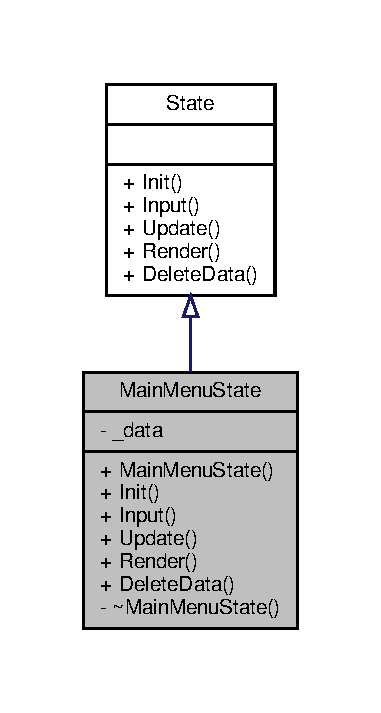
\includegraphics[width=183pt]{classMainMenuState__inherit__graph}
\end{center}
\end{figure}


Collaboration diagram for Main\+Menu\+State\+:
\nopagebreak
\begin{figure}[H]
\begin{center}
\leavevmode
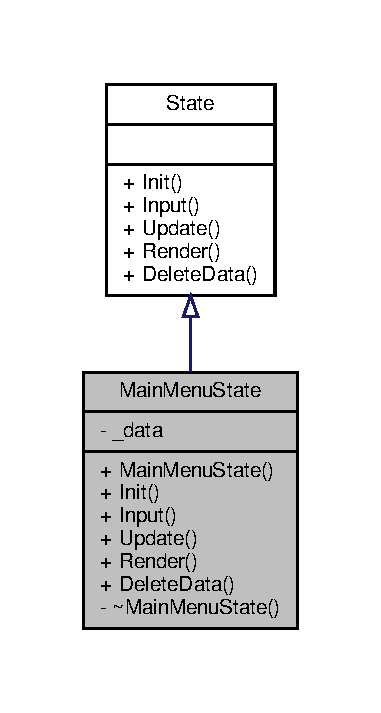
\includegraphics[width=183pt]{classMainMenuState__coll__graph}
\end{center}
\end{figure}
\subsection*{Public Member Functions}
\begin{DoxyCompactItemize}
\item 
\hyperlink{classMainMenuState_a8bf084041900c86967b51354fb26a230}{Main\+Menu\+State} (\hyperlink{game_8h_a513c9dd465a0df41dbb4daf40cc717c2}{Game\+Data\+Ref} data)
\item 
void \hyperlink{classMainMenuState_afab2a9b829a8ef752fed701d5cd260f8}{Init} ()
\item 
void \hyperlink{classMainMenuState_aa62c91d35b5b4a24c0a13c22020845e8}{Input} (float delta)
\item 
void \hyperlink{classMainMenuState_a1605be0d2e5228643d911c7069db3196}{Update} (float delta)
\item 
void \hyperlink{classMainMenuState_af675ec319923f1cf22446808a7735dea}{Render} (float delta)
\item 
void \hyperlink{classMainMenuState_a52c4dad229a1e9851e8742b81bc30abb}{Delete\+Data} ()
\end{DoxyCompactItemize}
\subsection*{Private Member Functions}
\begin{DoxyCompactItemize}
\item 
\hyperlink{classMainMenuState_a8af4d586b93c315a1a15b5fe83ec0760}{$\sim$\+Main\+Menu\+State} ()
\end{DoxyCompactItemize}
\subsection*{Private Attributes}
\begin{DoxyCompactItemize}
\item 
\hyperlink{game_8h_a513c9dd465a0df41dbb4daf40cc717c2}{Game\+Data\+Ref} \hyperlink{classMainMenuState_aa92b097f34007a1fc8223aa43062af46}{\+\_\+data}
\end{DoxyCompactItemize}


\subsection{Constructor \& Destructor Documentation}
\mbox{\Hypertarget{classMainMenuState_a8bf084041900c86967b51354fb26a230}\label{classMainMenuState_a8bf084041900c86967b51354fb26a230}} 
\index{Main\+Menu\+State@{Main\+Menu\+State}!Main\+Menu\+State@{Main\+Menu\+State}}
\index{Main\+Menu\+State@{Main\+Menu\+State}!Main\+Menu\+State@{Main\+Menu\+State}}
\subsubsection{\texorpdfstring{Main\+Menu\+State()}{MainMenuState()}}
{\footnotesize\ttfamily Main\+Menu\+State\+::\+Main\+Menu\+State (\begin{DoxyParamCaption}\item[{\hyperlink{game_8h_a513c9dd465a0df41dbb4daf40cc717c2}{Game\+Data\+Ref}}]{data }\end{DoxyParamCaption})}

\mbox{\Hypertarget{classMainMenuState_a8af4d586b93c315a1a15b5fe83ec0760}\label{classMainMenuState_a8af4d586b93c315a1a15b5fe83ec0760}} 
\index{Main\+Menu\+State@{Main\+Menu\+State}!````~Main\+Menu\+State@{$\sim$\+Main\+Menu\+State}}
\index{````~Main\+Menu\+State@{$\sim$\+Main\+Menu\+State}!Main\+Menu\+State@{Main\+Menu\+State}}
\subsubsection{\texorpdfstring{$\sim$\+Main\+Menu\+State()}{~MainMenuState()}}
{\footnotesize\ttfamily Main\+Menu\+State\+::$\sim$\+Main\+Menu\+State (\begin{DoxyParamCaption}{ }\end{DoxyParamCaption})\hspace{0.3cm}{\ttfamily [private]}}



\subsection{Member Function Documentation}
\mbox{\Hypertarget{classMainMenuState_a52c4dad229a1e9851e8742b81bc30abb}\label{classMainMenuState_a52c4dad229a1e9851e8742b81bc30abb}} 
\index{Main\+Menu\+State@{Main\+Menu\+State}!Delete\+Data@{Delete\+Data}}
\index{Delete\+Data@{Delete\+Data}!Main\+Menu\+State@{Main\+Menu\+State}}
\subsubsection{\texorpdfstring{Delete\+Data()}{DeleteData()}}
{\footnotesize\ttfamily void Main\+Menu\+State\+::\+Delete\+Data (\begin{DoxyParamCaption}{ }\end{DoxyParamCaption})\hspace{0.3cm}{\ttfamily [virtual]}}



Implements \hyperlink{classState_ade502eaa386d570e526eb356ffd73fd8}{State}.

\mbox{\Hypertarget{classMainMenuState_afab2a9b829a8ef752fed701d5cd260f8}\label{classMainMenuState_afab2a9b829a8ef752fed701d5cd260f8}} 
\index{Main\+Menu\+State@{Main\+Menu\+State}!Init@{Init}}
\index{Init@{Init}!Main\+Menu\+State@{Main\+Menu\+State}}
\subsubsection{\texorpdfstring{Init()}{Init()}}
{\footnotesize\ttfamily void Main\+Menu\+State\+::\+Init (\begin{DoxyParamCaption}{ }\end{DoxyParamCaption})\hspace{0.3cm}{\ttfamily [virtual]}}



Implements \hyperlink{classState_a7ab4d8c6aa239a17ed579d89a209b156}{State}.

\mbox{\Hypertarget{classMainMenuState_aa62c91d35b5b4a24c0a13c22020845e8}\label{classMainMenuState_aa62c91d35b5b4a24c0a13c22020845e8}} 
\index{Main\+Menu\+State@{Main\+Menu\+State}!Input@{Input}}
\index{Input@{Input}!Main\+Menu\+State@{Main\+Menu\+State}}
\subsubsection{\texorpdfstring{Input()}{Input()}}
{\footnotesize\ttfamily void Main\+Menu\+State\+::\+Input (\begin{DoxyParamCaption}\item[{float}]{delta }\end{DoxyParamCaption})\hspace{0.3cm}{\ttfamily [virtual]}}



Implements \hyperlink{classState_a1705412877f37a5cc8fc712542756076}{State}.

\mbox{\Hypertarget{classMainMenuState_af675ec319923f1cf22446808a7735dea}\label{classMainMenuState_af675ec319923f1cf22446808a7735dea}} 
\index{Main\+Menu\+State@{Main\+Menu\+State}!Render@{Render}}
\index{Render@{Render}!Main\+Menu\+State@{Main\+Menu\+State}}
\subsubsection{\texorpdfstring{Render()}{Render()}}
{\footnotesize\ttfamily void Main\+Menu\+State\+::\+Render (\begin{DoxyParamCaption}\item[{float}]{delta }\end{DoxyParamCaption})\hspace{0.3cm}{\ttfamily [virtual]}}



Implements \hyperlink{classState_a0e48dfae1e3090630475812681417c5f}{State}.

\mbox{\Hypertarget{classMainMenuState_a1605be0d2e5228643d911c7069db3196}\label{classMainMenuState_a1605be0d2e5228643d911c7069db3196}} 
\index{Main\+Menu\+State@{Main\+Menu\+State}!Update@{Update}}
\index{Update@{Update}!Main\+Menu\+State@{Main\+Menu\+State}}
\subsubsection{\texorpdfstring{Update()}{Update()}}
{\footnotesize\ttfamily void Main\+Menu\+State\+::\+Update (\begin{DoxyParamCaption}\item[{float}]{delta }\end{DoxyParamCaption})\hspace{0.3cm}{\ttfamily [virtual]}}



Implements \hyperlink{classState_aac0d3fdee1341e168af730b8f31a7bf1}{State}.



\subsection{Member Data Documentation}
\mbox{\Hypertarget{classMainMenuState_aa92b097f34007a1fc8223aa43062af46}\label{classMainMenuState_aa92b097f34007a1fc8223aa43062af46}} 
\index{Main\+Menu\+State@{Main\+Menu\+State}!\+\_\+data@{\+\_\+data}}
\index{\+\_\+data@{\+\_\+data}!Main\+Menu\+State@{Main\+Menu\+State}}
\subsubsection{\texorpdfstring{\+\_\+data}{\_data}}
{\footnotesize\ttfamily \hyperlink{game_8h_a513c9dd465a0df41dbb4daf40cc717c2}{Game\+Data\+Ref} Main\+Menu\+State\+::\+\_\+data\hspace{0.3cm}{\ttfamily [private]}}



The documentation for this class was generated from the following files\+:\begin{DoxyCompactItemize}
\item 
/mnt/hdd/\+C0de/smart\+\_\+engine/include/\hyperlink{main__menu__state_8h}{main\+\_\+menu\+\_\+state.\+h}\item 
/mnt/hdd/\+C0de/smart\+\_\+engine/src/\hyperlink{main__menu__state_8cpp}{main\+\_\+menu\+\_\+state.\+cpp}\end{DoxyCompactItemize}

\hypertarget{classmap}{}\section{map Class Reference}
\label{classmap}\index{map@{map}}


Collaboration diagram for map\+:
\nopagebreak
\begin{figure}[H]
\begin{center}
\leavevmode
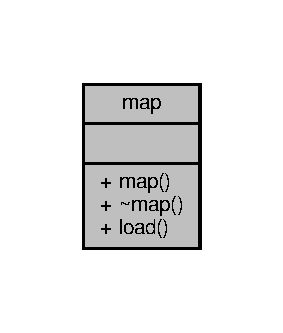
\includegraphics[width=136pt]{classmap__coll__graph}
\end{center}
\end{figure}
\subsection*{Public Member Functions}
\begin{DoxyCompactItemize}
\item 
\hyperlink{classmap_abedfe6722ad83929739afd899c88fea4}{map} ()
\item 
\hyperlink{classmap_a0cc22df7b44f7835fa10ed241848b041}{$\sim$map} ()
\item 
void \hyperlink{classmap_a3edebf1c088adbb83a2e412accbe998e}{load} (std\+::string file\+Path)
\end{DoxyCompactItemize}


\subsection{Constructor \& Destructor Documentation}
\mbox{\Hypertarget{classmap_abedfe6722ad83929739afd899c88fea4}\label{classmap_abedfe6722ad83929739afd899c88fea4}} 
\index{map@{map}!map@{map}}
\index{map@{map}!map@{map}}
\subsubsection{\texorpdfstring{map()}{map()}}
{\footnotesize\ttfamily map\+::map (\begin{DoxyParamCaption}{ }\end{DoxyParamCaption})\hspace{0.3cm}{\ttfamily [inline]}}

\mbox{\Hypertarget{classmap_a0cc22df7b44f7835fa10ed241848b041}\label{classmap_a0cc22df7b44f7835fa10ed241848b041}} 
\index{map@{map}!````~map@{$\sim$map}}
\index{````~map@{$\sim$map}!map@{map}}
\subsubsection{\texorpdfstring{$\sim$map()}{~map()}}
{\footnotesize\ttfamily map\+::$\sim$map (\begin{DoxyParamCaption}{ }\end{DoxyParamCaption})\hspace{0.3cm}{\ttfamily [inline]}}



\subsection{Member Function Documentation}
\mbox{\Hypertarget{classmap_a3edebf1c088adbb83a2e412accbe998e}\label{classmap_a3edebf1c088adbb83a2e412accbe998e}} 
\index{map@{map}!load@{load}}
\index{load@{load}!map@{map}}
\subsubsection{\texorpdfstring{load()}{load()}}
{\footnotesize\ttfamily void map\+::load (\begin{DoxyParamCaption}\item[{std\+::string}]{file\+Path }\end{DoxyParamCaption})\hspace{0.3cm}{\ttfamily [inline]}}



The documentation for this class was generated from the following file\+:\begin{DoxyCompactItemize}
\item 
/mnt/hdd/\+C0de/smart\+\_\+engine/src/\hyperlink{map_8cpp}{map.\+cpp}\end{DoxyCompactItemize}

\hypertarget{classMapLayer}{}\section{Map\+Layer Class Reference}
\label{classMapLayer}\index{Map\+Layer@{Map\+Layer}}


{\ttfamily \#include $<$S\+F\+M\+L\+Orthogonal\+Layer.\+hpp$>$}



Inheritance diagram for Map\+Layer\+:
\nopagebreak
\begin{figure}[H]
\begin{center}
\leavevmode
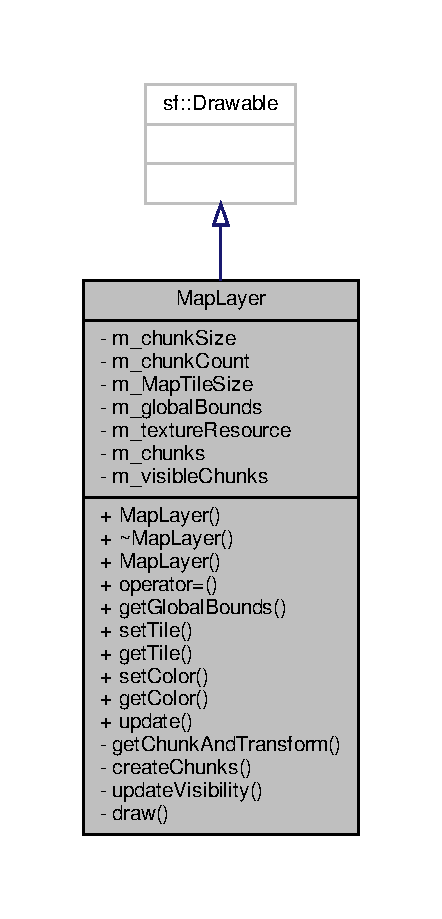
\includegraphics[width=212pt]{classMapLayer__inherit__graph}
\end{center}
\end{figure}


Collaboration diagram for Map\+Layer\+:
\nopagebreak
\begin{figure}[H]
\begin{center}
\leavevmode
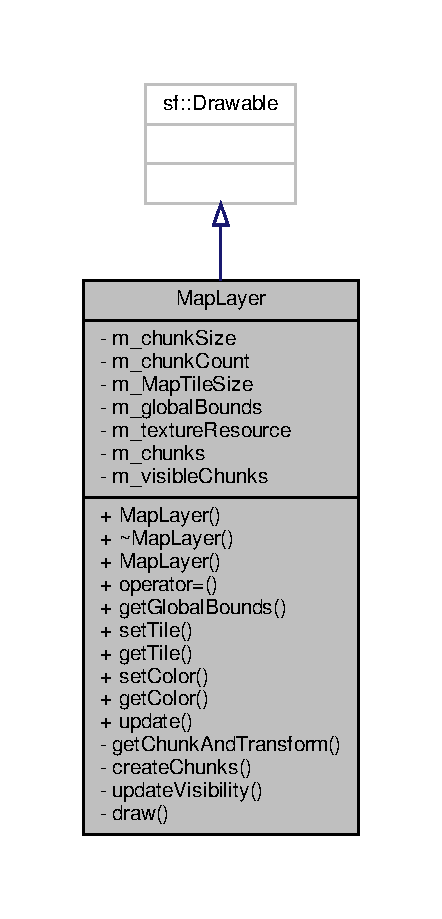
\includegraphics[width=212pt]{classMapLayer__coll__graph}
\end{center}
\end{figure}
\subsection*{Classes}
\begin{DoxyCompactItemize}
\item 
struct \hyperlink{structMapLayer_1_1AnimationState}{Animation\+State}
\item 
class \hyperlink{classMapLayer_1_1Chunk}{Chunk}
\end{DoxyCompactItemize}
\subsection*{Public Member Functions}
\begin{DoxyCompactItemize}
\item 
\hyperlink{classMapLayer_ac1b9f1e3ba6d800abf508fa11490187b}{Map\+Layer} (const tmx\+::\+Map \&map, std\+::size\+\_\+t idx)
\item 
\hyperlink{classMapLayer_a79858f9ee05242aa47ac680940e5ea74}{$\sim$\+Map\+Layer} ()=default
\item 
\hyperlink{classMapLayer_af323ddae8da169a64be1e0c216034397}{Map\+Layer} (const \hyperlink{classMapLayer}{Map\+Layer} \&)=delete
\item 
\hyperlink{classMapLayer}{Map\+Layer} \& \hyperlink{classMapLayer_a1863f3842c104aa6d460f4d9b99ec792}{operator=} (const \hyperlink{classMapLayer}{Map\+Layer} \&)=delete
\item 
const sf\+::\+Float\+Rect \& \hyperlink{classMapLayer_ae87bc38c7c030e9b2822b53f6de13d13}{get\+Global\+Bounds} () const
\item 
void \hyperlink{classMapLayer_a1152792435a0fa6203f6c3a038b93778}{set\+Tile} (int tileX, int tileY, tmx\+::\+Tile\+Layer\+::\+Tile tile, bool refresh=true)
\item 
tmx\+::\+Tile\+Layer\+::\+Tile \hyperlink{classMapLayer_a347375abb72832ea3362ba0d29898f30}{get\+Tile} (int tileX, int tileY)
\item 
void \hyperlink{classMapLayer_a4dad5e08a823925292846664ce42657d}{set\+Color} (int tileX, int tileY, sf\+::\+Color color, bool refresh=true)
\item 
sf\+::\+Color \hyperlink{classMapLayer_a6ecfbaf968ac9e6e4f814a30aa0c0f30}{get\+Color} (int tileX, int tileY)
\item 
void \hyperlink{classMapLayer_a0f7690e23ecfde7a7dc6629f9df65635}{update} (sf\+::\+Time elapsed)
\end{DoxyCompactItemize}
\subsection*{Private Types}
\begin{DoxyCompactItemize}
\item 
using \hyperlink{classMapLayer_a64011087426e436e3cb8374570378d68}{Texture\+Resource} = std\+::map$<$ std\+::string, std\+::unique\+\_\+ptr$<$ sf\+::\+Texture $>$ $>$
\end{DoxyCompactItemize}
\subsection*{Private Member Functions}
\begin{DoxyCompactItemize}
\item 
\hyperlink{classMapLayer_1_1Chunk_ab1df4d3621c5d9f83c2edb46d0744078}{Chunk\+::\+Ptr} \& \hyperlink{classMapLayer_a5686d500c087caa0c096c965d5d36574}{get\+Chunk\+And\+Transform} (int x, int y, sf\+::\+Vector2u \&chunk\+Relative)
\item 
void \hyperlink{classMapLayer_a853b2091fa76fabe4446797e0a01809a}{create\+Chunks} (const tmx\+::\+Map \&map, const tmx\+::\+Tile\+Layer \&layer)
\item 
void \hyperlink{classMapLayer_a6602d1d89676fa73ace9934f7b77c0c5}{update\+Visibility} (const sf\+::\+View \&view) const
\item 
void \hyperlink{classMapLayer_a6a43405b98f14c3efbe02395c466c1e6}{draw} (sf\+::\+Render\+Target \&rt, sf\+::\+Render\+States states) const override
\end{DoxyCompactItemize}
\subsection*{Private Attributes}
\begin{DoxyCompactItemize}
\item 
sf\+::\+Vector2f \hyperlink{classMapLayer_af8d36b6ff112417b9d4f73a52e8859ae}{m\+\_\+chunk\+Size} = sf\+::\+Vector2f(512.f, 512.f)
\item 
sf\+::\+Vector2u \hyperlink{classMapLayer_ae816f79d9d81eb7e9e207c00bbf41218}{m\+\_\+chunk\+Count}
\item 
sf\+::\+Vector2u \hyperlink{classMapLayer_a9863689eb080d27e7a99dea7c20aee41}{m\+\_\+\+Map\+Tile\+Size}
\item 
sf\+::\+Float\+Rect \hyperlink{classMapLayer_a1e1ca5c4bedf393c1c85e2ced3bbf50a}{m\+\_\+global\+Bounds}
\item 
\hyperlink{classMapLayer_a64011087426e436e3cb8374570378d68}{Texture\+Resource} \hyperlink{classMapLayer_ad7cade67df5e55b3c6a960476e6d2cb9}{m\+\_\+texture\+Resource}
\item 
std\+::vector$<$ \hyperlink{classMapLayer_1_1Chunk_ab1df4d3621c5d9f83c2edb46d0744078}{Chunk\+::\+Ptr} $>$ \hyperlink{classMapLayer_a07e8acdbdfc63584a2b9276ca499ad70}{m\+\_\+chunks}
\item 
std\+::vector$<$ \hyperlink{classMapLayer_1_1Chunk}{Chunk} $\ast$ $>$ \hyperlink{classMapLayer_a74941b5479affea58ea8a3068770d430}{m\+\_\+visible\+Chunks}
\end{DoxyCompactItemize}


\subsection{Member Typedef Documentation}
\mbox{\Hypertarget{classMapLayer_a64011087426e436e3cb8374570378d68}\label{classMapLayer_a64011087426e436e3cb8374570378d68}} 
\index{Map\+Layer@{Map\+Layer}!Texture\+Resource@{Texture\+Resource}}
\index{Texture\+Resource@{Texture\+Resource}!Map\+Layer@{Map\+Layer}}
\subsubsection{\texorpdfstring{Texture\+Resource}{TextureResource}}
{\footnotesize\ttfamily using \hyperlink{classMapLayer_a64011087426e436e3cb8374570378d68}{Map\+Layer\+::\+Texture\+Resource} =  std\+::map$<$std\+::string, std\+::unique\+\_\+ptr$<$sf\+::\+Texture$>$ $>$\hspace{0.3cm}{\ttfamily [private]}}



\subsection{Constructor \& Destructor Documentation}
\mbox{\Hypertarget{classMapLayer_ac1b9f1e3ba6d800abf508fa11490187b}\label{classMapLayer_ac1b9f1e3ba6d800abf508fa11490187b}} 
\index{Map\+Layer@{Map\+Layer}!Map\+Layer@{Map\+Layer}}
\index{Map\+Layer@{Map\+Layer}!Map\+Layer@{Map\+Layer}}
\subsubsection{\texorpdfstring{Map\+Layer()}{MapLayer()}\hspace{0.1cm}{\footnotesize\ttfamily [1/2]}}
{\footnotesize\ttfamily Map\+Layer\+::\+Map\+Layer (\begin{DoxyParamCaption}\item[{const tmx\+::\+Map \&}]{map,  }\item[{std\+::size\+\_\+t}]{idx }\end{DoxyParamCaption})\hspace{0.3cm}{\ttfamily [inline]}}

\mbox{\Hypertarget{classMapLayer_a79858f9ee05242aa47ac680940e5ea74}\label{classMapLayer_a79858f9ee05242aa47ac680940e5ea74}} 
\index{Map\+Layer@{Map\+Layer}!````~Map\+Layer@{$\sim$\+Map\+Layer}}
\index{````~Map\+Layer@{$\sim$\+Map\+Layer}!Map\+Layer@{Map\+Layer}}
\subsubsection{\texorpdfstring{$\sim$\+Map\+Layer()}{~MapLayer()}}
{\footnotesize\ttfamily Map\+Layer\+::$\sim$\+Map\+Layer (\begin{DoxyParamCaption}{ }\end{DoxyParamCaption})\hspace{0.3cm}{\ttfamily [default]}}

\mbox{\Hypertarget{classMapLayer_af323ddae8da169a64be1e0c216034397}\label{classMapLayer_af323ddae8da169a64be1e0c216034397}} 
\index{Map\+Layer@{Map\+Layer}!Map\+Layer@{Map\+Layer}}
\index{Map\+Layer@{Map\+Layer}!Map\+Layer@{Map\+Layer}}
\subsubsection{\texorpdfstring{Map\+Layer()}{MapLayer()}\hspace{0.1cm}{\footnotesize\ttfamily [2/2]}}
{\footnotesize\ttfamily Map\+Layer\+::\+Map\+Layer (\begin{DoxyParamCaption}\item[{const \hyperlink{classMapLayer}{Map\+Layer} \&}]{ }\end{DoxyParamCaption})\hspace{0.3cm}{\ttfamily [delete]}}



\subsection{Member Function Documentation}
\mbox{\Hypertarget{classMapLayer_a853b2091fa76fabe4446797e0a01809a}\label{classMapLayer_a853b2091fa76fabe4446797e0a01809a}} 
\index{Map\+Layer@{Map\+Layer}!create\+Chunks@{create\+Chunks}}
\index{create\+Chunks@{create\+Chunks}!Map\+Layer@{Map\+Layer}}
\subsubsection{\texorpdfstring{create\+Chunks()}{createChunks()}}
{\footnotesize\ttfamily void Map\+Layer\+::create\+Chunks (\begin{DoxyParamCaption}\item[{const tmx\+::\+Map \&}]{map,  }\item[{const tmx\+::\+Tile\+Layer \&}]{layer }\end{DoxyParamCaption})\hspace{0.3cm}{\ttfamily [inline]}, {\ttfamily [private]}}

\mbox{\Hypertarget{classMapLayer_a6a43405b98f14c3efbe02395c466c1e6}\label{classMapLayer_a6a43405b98f14c3efbe02395c466c1e6}} 
\index{Map\+Layer@{Map\+Layer}!draw@{draw}}
\index{draw@{draw}!Map\+Layer@{Map\+Layer}}
\subsubsection{\texorpdfstring{draw()}{draw()}}
{\footnotesize\ttfamily void Map\+Layer\+::draw (\begin{DoxyParamCaption}\item[{sf\+::\+Render\+Target \&}]{rt,  }\item[{sf\+::\+Render\+States}]{states }\end{DoxyParamCaption}) const\hspace{0.3cm}{\ttfamily [inline]}, {\ttfamily [override]}, {\ttfamily [private]}}

\mbox{\Hypertarget{classMapLayer_a5686d500c087caa0c096c965d5d36574}\label{classMapLayer_a5686d500c087caa0c096c965d5d36574}} 
\index{Map\+Layer@{Map\+Layer}!get\+Chunk\+And\+Transform@{get\+Chunk\+And\+Transform}}
\index{get\+Chunk\+And\+Transform@{get\+Chunk\+And\+Transform}!Map\+Layer@{Map\+Layer}}
\subsubsection{\texorpdfstring{get\+Chunk\+And\+Transform()}{getChunkAndTransform()}}
{\footnotesize\ttfamily \hyperlink{classMapLayer_1_1Chunk_ab1df4d3621c5d9f83c2edb46d0744078}{Chunk\+::\+Ptr}\& Map\+Layer\+::get\+Chunk\+And\+Transform (\begin{DoxyParamCaption}\item[{int}]{x,  }\item[{int}]{y,  }\item[{sf\+::\+Vector2u \&}]{chunk\+Relative }\end{DoxyParamCaption})\hspace{0.3cm}{\ttfamily [inline]}, {\ttfamily [private]}}

\mbox{\Hypertarget{classMapLayer_a6ecfbaf968ac9e6e4f814a30aa0c0f30}\label{classMapLayer_a6ecfbaf968ac9e6e4f814a30aa0c0f30}} 
\index{Map\+Layer@{Map\+Layer}!get\+Color@{get\+Color}}
\index{get\+Color@{get\+Color}!Map\+Layer@{Map\+Layer}}
\subsubsection{\texorpdfstring{get\+Color()}{getColor()}}
{\footnotesize\ttfamily sf\+::\+Color Map\+Layer\+::get\+Color (\begin{DoxyParamCaption}\item[{int}]{tileX,  }\item[{int}]{tileY }\end{DoxyParamCaption})\hspace{0.3cm}{\ttfamily [inline]}}

\mbox{\Hypertarget{classMapLayer_ae87bc38c7c030e9b2822b53f6de13d13}\label{classMapLayer_ae87bc38c7c030e9b2822b53f6de13d13}} 
\index{Map\+Layer@{Map\+Layer}!get\+Global\+Bounds@{get\+Global\+Bounds}}
\index{get\+Global\+Bounds@{get\+Global\+Bounds}!Map\+Layer@{Map\+Layer}}
\subsubsection{\texorpdfstring{get\+Global\+Bounds()}{getGlobalBounds()}}
{\footnotesize\ttfamily const sf\+::\+Float\+Rect\& Map\+Layer\+::get\+Global\+Bounds (\begin{DoxyParamCaption}{ }\end{DoxyParamCaption}) const\hspace{0.3cm}{\ttfamily [inline]}}

\mbox{\Hypertarget{classMapLayer_a347375abb72832ea3362ba0d29898f30}\label{classMapLayer_a347375abb72832ea3362ba0d29898f30}} 
\index{Map\+Layer@{Map\+Layer}!get\+Tile@{get\+Tile}}
\index{get\+Tile@{get\+Tile}!Map\+Layer@{Map\+Layer}}
\subsubsection{\texorpdfstring{get\+Tile()}{getTile()}}
{\footnotesize\ttfamily tmx\+::\+Tile\+Layer\+::\+Tile Map\+Layer\+::get\+Tile (\begin{DoxyParamCaption}\item[{int}]{tileX,  }\item[{int}]{tileY }\end{DoxyParamCaption})\hspace{0.3cm}{\ttfamily [inline]}}

\mbox{\Hypertarget{classMapLayer_a1863f3842c104aa6d460f4d9b99ec792}\label{classMapLayer_a1863f3842c104aa6d460f4d9b99ec792}} 
\index{Map\+Layer@{Map\+Layer}!operator=@{operator=}}
\index{operator=@{operator=}!Map\+Layer@{Map\+Layer}}
\subsubsection{\texorpdfstring{operator=()}{operator=()}}
{\footnotesize\ttfamily \hyperlink{classMapLayer}{Map\+Layer}\& Map\+Layer\+::operator= (\begin{DoxyParamCaption}\item[{const \hyperlink{classMapLayer}{Map\+Layer} \&}]{ }\end{DoxyParamCaption})\hspace{0.3cm}{\ttfamily [delete]}}

\mbox{\Hypertarget{classMapLayer_a4dad5e08a823925292846664ce42657d}\label{classMapLayer_a4dad5e08a823925292846664ce42657d}} 
\index{Map\+Layer@{Map\+Layer}!set\+Color@{set\+Color}}
\index{set\+Color@{set\+Color}!Map\+Layer@{Map\+Layer}}
\subsubsection{\texorpdfstring{set\+Color()}{setColor()}}
{\footnotesize\ttfamily void Map\+Layer\+::set\+Color (\begin{DoxyParamCaption}\item[{int}]{tileX,  }\item[{int}]{tileY,  }\item[{sf\+::\+Color}]{color,  }\item[{bool}]{refresh = {\ttfamily true} }\end{DoxyParamCaption})\hspace{0.3cm}{\ttfamily [inline]}}

\mbox{\Hypertarget{classMapLayer_a1152792435a0fa6203f6c3a038b93778}\label{classMapLayer_a1152792435a0fa6203f6c3a038b93778}} 
\index{Map\+Layer@{Map\+Layer}!set\+Tile@{set\+Tile}}
\index{set\+Tile@{set\+Tile}!Map\+Layer@{Map\+Layer}}
\subsubsection{\texorpdfstring{set\+Tile()}{setTile()}}
{\footnotesize\ttfamily void Map\+Layer\+::set\+Tile (\begin{DoxyParamCaption}\item[{int}]{tileX,  }\item[{int}]{tileY,  }\item[{tmx\+::\+Tile\+Layer\+::\+Tile}]{tile,  }\item[{bool}]{refresh = {\ttfamily true} }\end{DoxyParamCaption})\hspace{0.3cm}{\ttfamily [inline]}}

\mbox{\Hypertarget{classMapLayer_a0f7690e23ecfde7a7dc6629f9df65635}\label{classMapLayer_a0f7690e23ecfde7a7dc6629f9df65635}} 
\index{Map\+Layer@{Map\+Layer}!update@{update}}
\index{update@{update}!Map\+Layer@{Map\+Layer}}
\subsubsection{\texorpdfstring{update()}{update()}}
{\footnotesize\ttfamily void Map\+Layer\+::update (\begin{DoxyParamCaption}\item[{sf\+::\+Time}]{elapsed }\end{DoxyParamCaption})\hspace{0.3cm}{\ttfamily [inline]}}

\mbox{\Hypertarget{classMapLayer_a6602d1d89676fa73ace9934f7b77c0c5}\label{classMapLayer_a6602d1d89676fa73ace9934f7b77c0c5}} 
\index{Map\+Layer@{Map\+Layer}!update\+Visibility@{update\+Visibility}}
\index{update\+Visibility@{update\+Visibility}!Map\+Layer@{Map\+Layer}}
\subsubsection{\texorpdfstring{update\+Visibility()}{updateVisibility()}}
{\footnotesize\ttfamily void Map\+Layer\+::update\+Visibility (\begin{DoxyParamCaption}\item[{const sf\+::\+View \&}]{view }\end{DoxyParamCaption}) const\hspace{0.3cm}{\ttfamily [inline]}, {\ttfamily [private]}}



\subsection{Member Data Documentation}
\mbox{\Hypertarget{classMapLayer_ae816f79d9d81eb7e9e207c00bbf41218}\label{classMapLayer_ae816f79d9d81eb7e9e207c00bbf41218}} 
\index{Map\+Layer@{Map\+Layer}!m\+\_\+chunk\+Count@{m\+\_\+chunk\+Count}}
\index{m\+\_\+chunk\+Count@{m\+\_\+chunk\+Count}!Map\+Layer@{Map\+Layer}}
\subsubsection{\texorpdfstring{m\+\_\+chunk\+Count}{m\_chunkCount}}
{\footnotesize\ttfamily sf\+::\+Vector2u Map\+Layer\+::m\+\_\+chunk\+Count\hspace{0.3cm}{\ttfamily [private]}}

\mbox{\Hypertarget{classMapLayer_a07e8acdbdfc63584a2b9276ca499ad70}\label{classMapLayer_a07e8acdbdfc63584a2b9276ca499ad70}} 
\index{Map\+Layer@{Map\+Layer}!m\+\_\+chunks@{m\+\_\+chunks}}
\index{m\+\_\+chunks@{m\+\_\+chunks}!Map\+Layer@{Map\+Layer}}
\subsubsection{\texorpdfstring{m\+\_\+chunks}{m\_chunks}}
{\footnotesize\ttfamily std\+::vector$<$\hyperlink{classMapLayer_1_1Chunk_ab1df4d3621c5d9f83c2edb46d0744078}{Chunk\+::\+Ptr}$>$ Map\+Layer\+::m\+\_\+chunks\hspace{0.3cm}{\ttfamily [private]}}

\mbox{\Hypertarget{classMapLayer_af8d36b6ff112417b9d4f73a52e8859ae}\label{classMapLayer_af8d36b6ff112417b9d4f73a52e8859ae}} 
\index{Map\+Layer@{Map\+Layer}!m\+\_\+chunk\+Size@{m\+\_\+chunk\+Size}}
\index{m\+\_\+chunk\+Size@{m\+\_\+chunk\+Size}!Map\+Layer@{Map\+Layer}}
\subsubsection{\texorpdfstring{m\+\_\+chunk\+Size}{m\_chunkSize}}
{\footnotesize\ttfamily sf\+::\+Vector2f Map\+Layer\+::m\+\_\+chunk\+Size = sf\+::\+Vector2f(512.f, 512.f)\hspace{0.3cm}{\ttfamily [private]}}

\mbox{\Hypertarget{classMapLayer_a1e1ca5c4bedf393c1c85e2ced3bbf50a}\label{classMapLayer_a1e1ca5c4bedf393c1c85e2ced3bbf50a}} 
\index{Map\+Layer@{Map\+Layer}!m\+\_\+global\+Bounds@{m\+\_\+global\+Bounds}}
\index{m\+\_\+global\+Bounds@{m\+\_\+global\+Bounds}!Map\+Layer@{Map\+Layer}}
\subsubsection{\texorpdfstring{m\+\_\+global\+Bounds}{m\_globalBounds}}
{\footnotesize\ttfamily sf\+::\+Float\+Rect Map\+Layer\+::m\+\_\+global\+Bounds\hspace{0.3cm}{\ttfamily [private]}}

\mbox{\Hypertarget{classMapLayer_a9863689eb080d27e7a99dea7c20aee41}\label{classMapLayer_a9863689eb080d27e7a99dea7c20aee41}} 
\index{Map\+Layer@{Map\+Layer}!m\+\_\+\+Map\+Tile\+Size@{m\+\_\+\+Map\+Tile\+Size}}
\index{m\+\_\+\+Map\+Tile\+Size@{m\+\_\+\+Map\+Tile\+Size}!Map\+Layer@{Map\+Layer}}
\subsubsection{\texorpdfstring{m\+\_\+\+Map\+Tile\+Size}{m\_MapTileSize}}
{\footnotesize\ttfamily sf\+::\+Vector2u Map\+Layer\+::m\+\_\+\+Map\+Tile\+Size\hspace{0.3cm}{\ttfamily [private]}}

\mbox{\Hypertarget{classMapLayer_ad7cade67df5e55b3c6a960476e6d2cb9}\label{classMapLayer_ad7cade67df5e55b3c6a960476e6d2cb9}} 
\index{Map\+Layer@{Map\+Layer}!m\+\_\+texture\+Resource@{m\+\_\+texture\+Resource}}
\index{m\+\_\+texture\+Resource@{m\+\_\+texture\+Resource}!Map\+Layer@{Map\+Layer}}
\subsubsection{\texorpdfstring{m\+\_\+texture\+Resource}{m\_textureResource}}
{\footnotesize\ttfamily \hyperlink{classMapLayer_a64011087426e436e3cb8374570378d68}{Texture\+Resource} Map\+Layer\+::m\+\_\+texture\+Resource\hspace{0.3cm}{\ttfamily [private]}}

\mbox{\Hypertarget{classMapLayer_a74941b5479affea58ea8a3068770d430}\label{classMapLayer_a74941b5479affea58ea8a3068770d430}} 
\index{Map\+Layer@{Map\+Layer}!m\+\_\+visible\+Chunks@{m\+\_\+visible\+Chunks}}
\index{m\+\_\+visible\+Chunks@{m\+\_\+visible\+Chunks}!Map\+Layer@{Map\+Layer}}
\subsubsection{\texorpdfstring{m\+\_\+visible\+Chunks}{m\_visibleChunks}}
{\footnotesize\ttfamily std\+::vector$<$\hyperlink{classMapLayer_1_1Chunk}{Chunk}$\ast$$>$ Map\+Layer\+::m\+\_\+visible\+Chunks\hspace{0.3cm}{\ttfamily [mutable]}, {\ttfamily [private]}}



The documentation for this class was generated from the following file\+:\begin{DoxyCompactItemize}
\item 
/mnt/hdd/\+C0de/\+Engines/\+S\+F\+M\+L/\+S\+F\+M\+L\+\_\+\+Engine/include/\hyperlink{SFMLOrthogonalLayer_8hpp}{S\+F\+M\+L\+Orthogonal\+Layer.\+hpp}\end{DoxyCompactItemize}

\hypertarget{classOrthographic__camera}{}\section{Orthographic\+\_\+camera Class Reference}
\label{classOrthographic__camera}\index{Orthographic\+\_\+camera@{Orthographic\+\_\+camera}}


{\ttfamily \#include $<$Orthographic\+\_\+camera.\+h$>$}



Collaboration diagram for Orthographic\+\_\+camera\+:
\nopagebreak
\begin{figure}[H]
\begin{center}
\leavevmode
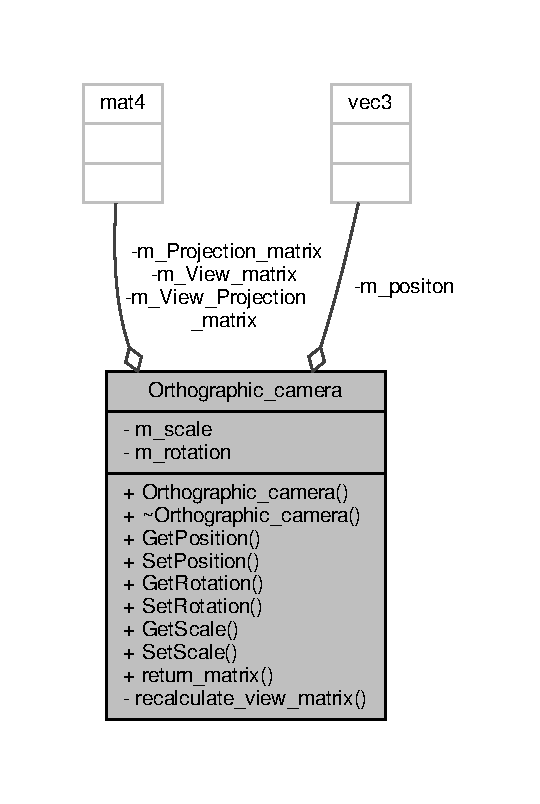
\includegraphics[width=259pt]{classOrthographic__camera__coll__graph}
\end{center}
\end{figure}
\subsection*{Public Member Functions}
\begin{DoxyCompactItemize}
\item 
\hyperlink{classOrthographic__camera_aeb45b5f12a351769d0b80a2926193e7f}{Orthographic\+\_\+camera} (float left, float right, float bottom, float top, float z\+Near, float z\+Far)
\item 
\hyperlink{classOrthographic__camera_abd3ea1d0674fc8de61786ff787d97390}{$\sim$\+Orthographic\+\_\+camera} ()
\item 
const glm\+::vec3 \& \hyperlink{classOrthographic__camera_aae41cb7e5c48eb6ce5354d86c9d13123}{Get\+Position} () const
\item 
void \hyperlink{classOrthographic__camera_a3cf573e0cc2b494bf6ca7adf11df8d0f}{Set\+Position} (const glm\+::vec3 position)
\item 
float \hyperlink{classOrthographic__camera_a8c9169569698fca75d45550b0cf450b3}{Get\+Rotation} () const
\item 
void \hyperlink{classOrthographic__camera_aafb33c86e3b3178dd76192e72306f1fb}{Set\+Rotation} (float rotation)
\item 
const glm\+::vec2 \& \hyperlink{classOrthographic__camera_a6e6a3c646d9f677e2522671b0c0f1ce0}{Get\+Scale} () const
\item 
void \hyperlink{classOrthographic__camera_ac3975aafe2fc108abf27a9df0068dd56}{Set\+Scale} (glm\+::vec2 z\+\_\+scale)
\item 
glm\+::mat4 \hyperlink{classOrthographic__camera_ac8140eaa2011ecc0a7fb80ca38111909}{return\+\_\+matrix} ()
\end{DoxyCompactItemize}
\subsection*{Private Member Functions}
\begin{DoxyCompactItemize}
\item 
void \hyperlink{classOrthographic__camera_aa878ce1cd32947da29852ea03dcffd01}{recalculate\+\_\+view\+\_\+matrix} ()
\end{DoxyCompactItemize}
\subsection*{Private Attributes}
\begin{DoxyCompactItemize}
\item 
glm\+::mat4 \hyperlink{classOrthographic__camera_ab86fab9f0ee868e8cca74ded191c4ab9}{m\+\_\+\+Projection\+\_\+matrix}
\item 
glm\+::mat4 \hyperlink{classOrthographic__camera_aadb603c787908e6b7545baa3367dd0bc}{m\+\_\+\+View\+\_\+matrix}
\item 
glm\+::mat4 \hyperlink{classOrthographic__camera_a3826c2d1b6976581f2d3288432f1b62a}{m\+\_\+\+View\+\_\+\+Projection\+\_\+matrix}
\item 
glm\+::vec3 \hyperlink{classOrthographic__camera_a8ed8a2734597964dea167e5e212174b6}{m\+\_\+positon}
\item 
glm\+::vec2 \hyperlink{classOrthographic__camera_ad26f470c0fc6a7bb4394ddb9b4f9a55f}{m\+\_\+scale}
\item 
float \hyperlink{classOrthographic__camera_aae32e53691911da1651e4fdb82135951}{m\+\_\+rotation} = 0.\+0f
\end{DoxyCompactItemize}


\subsection{Constructor \& Destructor Documentation}
\mbox{\Hypertarget{classOrthographic__camera_aeb45b5f12a351769d0b80a2926193e7f}\label{classOrthographic__camera_aeb45b5f12a351769d0b80a2926193e7f}} 
\index{Orthographic\+\_\+camera@{Orthographic\+\_\+camera}!Orthographic\+\_\+camera@{Orthographic\+\_\+camera}}
\index{Orthographic\+\_\+camera@{Orthographic\+\_\+camera}!Orthographic\+\_\+camera@{Orthographic\+\_\+camera}}
\subsubsection{\texorpdfstring{Orthographic\+\_\+camera()}{Orthographic\_camera()}}
{\footnotesize\ttfamily Orthographic\+\_\+camera\+::\+Orthographic\+\_\+camera (\begin{DoxyParamCaption}\item[{float}]{left,  }\item[{float}]{right,  }\item[{float}]{bottom,  }\item[{float}]{top,  }\item[{float}]{z\+Near,  }\item[{float}]{z\+Far }\end{DoxyParamCaption})}

\mbox{\Hypertarget{classOrthographic__camera_abd3ea1d0674fc8de61786ff787d97390}\label{classOrthographic__camera_abd3ea1d0674fc8de61786ff787d97390}} 
\index{Orthographic\+\_\+camera@{Orthographic\+\_\+camera}!````~Orthographic\+\_\+camera@{$\sim$\+Orthographic\+\_\+camera}}
\index{````~Orthographic\+\_\+camera@{$\sim$\+Orthographic\+\_\+camera}!Orthographic\+\_\+camera@{Orthographic\+\_\+camera}}
\subsubsection{\texorpdfstring{$\sim$\+Orthographic\+\_\+camera()}{~Orthographic\_camera()}}
{\footnotesize\ttfamily Orthographic\+\_\+camera\+::$\sim$\+Orthographic\+\_\+camera (\begin{DoxyParamCaption}{ }\end{DoxyParamCaption})\hspace{0.3cm}{\ttfamily [inline]}}



\subsection{Member Function Documentation}
\mbox{\Hypertarget{classOrthographic__camera_aae41cb7e5c48eb6ce5354d86c9d13123}\label{classOrthographic__camera_aae41cb7e5c48eb6ce5354d86c9d13123}} 
\index{Orthographic\+\_\+camera@{Orthographic\+\_\+camera}!Get\+Position@{Get\+Position}}
\index{Get\+Position@{Get\+Position}!Orthographic\+\_\+camera@{Orthographic\+\_\+camera}}
\subsubsection{\texorpdfstring{Get\+Position()}{GetPosition()}}
{\footnotesize\ttfamily const glm\+::vec3\& Orthographic\+\_\+camera\+::\+Get\+Position (\begin{DoxyParamCaption}{ }\end{DoxyParamCaption}) const\hspace{0.3cm}{\ttfamily [inline]}}

\mbox{\Hypertarget{classOrthographic__camera_a8c9169569698fca75d45550b0cf450b3}\label{classOrthographic__camera_a8c9169569698fca75d45550b0cf450b3}} 
\index{Orthographic\+\_\+camera@{Orthographic\+\_\+camera}!Get\+Rotation@{Get\+Rotation}}
\index{Get\+Rotation@{Get\+Rotation}!Orthographic\+\_\+camera@{Orthographic\+\_\+camera}}
\subsubsection{\texorpdfstring{Get\+Rotation()}{GetRotation()}}
{\footnotesize\ttfamily float Orthographic\+\_\+camera\+::\+Get\+Rotation (\begin{DoxyParamCaption}{ }\end{DoxyParamCaption}) const\hspace{0.3cm}{\ttfamily [inline]}}

\mbox{\Hypertarget{classOrthographic__camera_a6e6a3c646d9f677e2522671b0c0f1ce0}\label{classOrthographic__camera_a6e6a3c646d9f677e2522671b0c0f1ce0}} 
\index{Orthographic\+\_\+camera@{Orthographic\+\_\+camera}!Get\+Scale@{Get\+Scale}}
\index{Get\+Scale@{Get\+Scale}!Orthographic\+\_\+camera@{Orthographic\+\_\+camera}}
\subsubsection{\texorpdfstring{Get\+Scale()}{GetScale()}}
{\footnotesize\ttfamily const glm\+::vec2\& Orthographic\+\_\+camera\+::\+Get\+Scale (\begin{DoxyParamCaption}{ }\end{DoxyParamCaption}) const\hspace{0.3cm}{\ttfamily [inline]}}

\mbox{\Hypertarget{classOrthographic__camera_aa878ce1cd32947da29852ea03dcffd01}\label{classOrthographic__camera_aa878ce1cd32947da29852ea03dcffd01}} 
\index{Orthographic\+\_\+camera@{Orthographic\+\_\+camera}!recalculate\+\_\+view\+\_\+matrix@{recalculate\+\_\+view\+\_\+matrix}}
\index{recalculate\+\_\+view\+\_\+matrix@{recalculate\+\_\+view\+\_\+matrix}!Orthographic\+\_\+camera@{Orthographic\+\_\+camera}}
\subsubsection{\texorpdfstring{recalculate\+\_\+view\+\_\+matrix()}{recalculate\_view\_matrix()}}
{\footnotesize\ttfamily void Orthographic\+\_\+camera\+::recalculate\+\_\+view\+\_\+matrix (\begin{DoxyParamCaption}{ }\end{DoxyParamCaption})\hspace{0.3cm}{\ttfamily [private]}}

\mbox{\Hypertarget{classOrthographic__camera_ac8140eaa2011ecc0a7fb80ca38111909}\label{classOrthographic__camera_ac8140eaa2011ecc0a7fb80ca38111909}} 
\index{Orthographic\+\_\+camera@{Orthographic\+\_\+camera}!return\+\_\+matrix@{return\+\_\+matrix}}
\index{return\+\_\+matrix@{return\+\_\+matrix}!Orthographic\+\_\+camera@{Orthographic\+\_\+camera}}
\subsubsection{\texorpdfstring{return\+\_\+matrix()}{return\_matrix()}}
{\footnotesize\ttfamily glm\+::mat4 Orthographic\+\_\+camera\+::return\+\_\+matrix (\begin{DoxyParamCaption}{ }\end{DoxyParamCaption})\hspace{0.3cm}{\ttfamily [inline]}}

\mbox{\Hypertarget{classOrthographic__camera_a3cf573e0cc2b494bf6ca7adf11df8d0f}\label{classOrthographic__camera_a3cf573e0cc2b494bf6ca7adf11df8d0f}} 
\index{Orthographic\+\_\+camera@{Orthographic\+\_\+camera}!Set\+Position@{Set\+Position}}
\index{Set\+Position@{Set\+Position}!Orthographic\+\_\+camera@{Orthographic\+\_\+camera}}
\subsubsection{\texorpdfstring{Set\+Position()}{SetPosition()}}
{\footnotesize\ttfamily void Orthographic\+\_\+camera\+::\+Set\+Position (\begin{DoxyParamCaption}\item[{const glm\+::vec3}]{position }\end{DoxyParamCaption})\hspace{0.3cm}{\ttfamily [inline]}}

\mbox{\Hypertarget{classOrthographic__camera_aafb33c86e3b3178dd76192e72306f1fb}\label{classOrthographic__camera_aafb33c86e3b3178dd76192e72306f1fb}} 
\index{Orthographic\+\_\+camera@{Orthographic\+\_\+camera}!Set\+Rotation@{Set\+Rotation}}
\index{Set\+Rotation@{Set\+Rotation}!Orthographic\+\_\+camera@{Orthographic\+\_\+camera}}
\subsubsection{\texorpdfstring{Set\+Rotation()}{SetRotation()}}
{\footnotesize\ttfamily void Orthographic\+\_\+camera\+::\+Set\+Rotation (\begin{DoxyParamCaption}\item[{float}]{rotation }\end{DoxyParamCaption})\hspace{0.3cm}{\ttfamily [inline]}}

\mbox{\Hypertarget{classOrthographic__camera_ac3975aafe2fc108abf27a9df0068dd56}\label{classOrthographic__camera_ac3975aafe2fc108abf27a9df0068dd56}} 
\index{Orthographic\+\_\+camera@{Orthographic\+\_\+camera}!Set\+Scale@{Set\+Scale}}
\index{Set\+Scale@{Set\+Scale}!Orthographic\+\_\+camera@{Orthographic\+\_\+camera}}
\subsubsection{\texorpdfstring{Set\+Scale()}{SetScale()}}
{\footnotesize\ttfamily void Orthographic\+\_\+camera\+::\+Set\+Scale (\begin{DoxyParamCaption}\item[{glm\+::vec2}]{z\+\_\+scale }\end{DoxyParamCaption})\hspace{0.3cm}{\ttfamily [inline]}}



\subsection{Member Data Documentation}
\mbox{\Hypertarget{classOrthographic__camera_a8ed8a2734597964dea167e5e212174b6}\label{classOrthographic__camera_a8ed8a2734597964dea167e5e212174b6}} 
\index{Orthographic\+\_\+camera@{Orthographic\+\_\+camera}!m\+\_\+positon@{m\+\_\+positon}}
\index{m\+\_\+positon@{m\+\_\+positon}!Orthographic\+\_\+camera@{Orthographic\+\_\+camera}}
\subsubsection{\texorpdfstring{m\+\_\+positon}{m\_positon}}
{\footnotesize\ttfamily glm\+::vec3 Orthographic\+\_\+camera\+::m\+\_\+positon\hspace{0.3cm}{\ttfamily [private]}}

\mbox{\Hypertarget{classOrthographic__camera_ab86fab9f0ee868e8cca74ded191c4ab9}\label{classOrthographic__camera_ab86fab9f0ee868e8cca74ded191c4ab9}} 
\index{Orthographic\+\_\+camera@{Orthographic\+\_\+camera}!m\+\_\+\+Projection\+\_\+matrix@{m\+\_\+\+Projection\+\_\+matrix}}
\index{m\+\_\+\+Projection\+\_\+matrix@{m\+\_\+\+Projection\+\_\+matrix}!Orthographic\+\_\+camera@{Orthographic\+\_\+camera}}
\subsubsection{\texorpdfstring{m\+\_\+\+Projection\+\_\+matrix}{m\_Projection\_matrix}}
{\footnotesize\ttfamily glm\+::mat4 Orthographic\+\_\+camera\+::m\+\_\+\+Projection\+\_\+matrix\hspace{0.3cm}{\ttfamily [private]}}

\mbox{\Hypertarget{classOrthographic__camera_aae32e53691911da1651e4fdb82135951}\label{classOrthographic__camera_aae32e53691911da1651e4fdb82135951}} 
\index{Orthographic\+\_\+camera@{Orthographic\+\_\+camera}!m\+\_\+rotation@{m\+\_\+rotation}}
\index{m\+\_\+rotation@{m\+\_\+rotation}!Orthographic\+\_\+camera@{Orthographic\+\_\+camera}}
\subsubsection{\texorpdfstring{m\+\_\+rotation}{m\_rotation}}
{\footnotesize\ttfamily float Orthographic\+\_\+camera\+::m\+\_\+rotation = 0.\+0f\hspace{0.3cm}{\ttfamily [private]}}

\mbox{\Hypertarget{classOrthographic__camera_ad26f470c0fc6a7bb4394ddb9b4f9a55f}\label{classOrthographic__camera_ad26f470c0fc6a7bb4394ddb9b4f9a55f}} 
\index{Orthographic\+\_\+camera@{Orthographic\+\_\+camera}!m\+\_\+scale@{m\+\_\+scale}}
\index{m\+\_\+scale@{m\+\_\+scale}!Orthographic\+\_\+camera@{Orthographic\+\_\+camera}}
\subsubsection{\texorpdfstring{m\+\_\+scale}{m\_scale}}
{\footnotesize\ttfamily glm\+::vec2 Orthographic\+\_\+camera\+::m\+\_\+scale\hspace{0.3cm}{\ttfamily [private]}}

\mbox{\Hypertarget{classOrthographic__camera_aadb603c787908e6b7545baa3367dd0bc}\label{classOrthographic__camera_aadb603c787908e6b7545baa3367dd0bc}} 
\index{Orthographic\+\_\+camera@{Orthographic\+\_\+camera}!m\+\_\+\+View\+\_\+matrix@{m\+\_\+\+View\+\_\+matrix}}
\index{m\+\_\+\+View\+\_\+matrix@{m\+\_\+\+View\+\_\+matrix}!Orthographic\+\_\+camera@{Orthographic\+\_\+camera}}
\subsubsection{\texorpdfstring{m\+\_\+\+View\+\_\+matrix}{m\_View\_matrix}}
{\footnotesize\ttfamily glm\+::mat4 Orthographic\+\_\+camera\+::m\+\_\+\+View\+\_\+matrix\hspace{0.3cm}{\ttfamily [private]}}

\mbox{\Hypertarget{classOrthographic__camera_a3826c2d1b6976581f2d3288432f1b62a}\label{classOrthographic__camera_a3826c2d1b6976581f2d3288432f1b62a}} 
\index{Orthographic\+\_\+camera@{Orthographic\+\_\+camera}!m\+\_\+\+View\+\_\+\+Projection\+\_\+matrix@{m\+\_\+\+View\+\_\+\+Projection\+\_\+matrix}}
\index{m\+\_\+\+View\+\_\+\+Projection\+\_\+matrix@{m\+\_\+\+View\+\_\+\+Projection\+\_\+matrix}!Orthographic\+\_\+camera@{Orthographic\+\_\+camera}}
\subsubsection{\texorpdfstring{m\+\_\+\+View\+\_\+\+Projection\+\_\+matrix}{m\_View\_Projection\_matrix}}
{\footnotesize\ttfamily glm\+::mat4 Orthographic\+\_\+camera\+::m\+\_\+\+View\+\_\+\+Projection\+\_\+matrix\hspace{0.3cm}{\ttfamily [private]}}



The documentation for this class was generated from the following files\+:\begin{DoxyCompactItemize}
\item 
/mnt/hdd/\+C0de/smart\+\_\+engine/include/\hyperlink{Orthographic__camera_8h}{Orthographic\+\_\+camera.\+h}\item 
/mnt/hdd/\+C0de/smart\+\_\+engine/src/\hyperlink{Orthographic__camera_8cpp}{Orthographic\+\_\+camera.\+cpp}\end{DoxyCompactItemize}

\hypertarget{classResourceManager}{}\section{Resource\+Manager Class Reference}
\label{classResourceManager}\index{Resource\+Manager@{Resource\+Manager}}


{\ttfamily \#include $<$resource\+\_\+manager.\+h$>$}



Collaboration diagram for Resource\+Manager\+:
\nopagebreak
\begin{figure}[H]
\begin{center}
\leavevmode
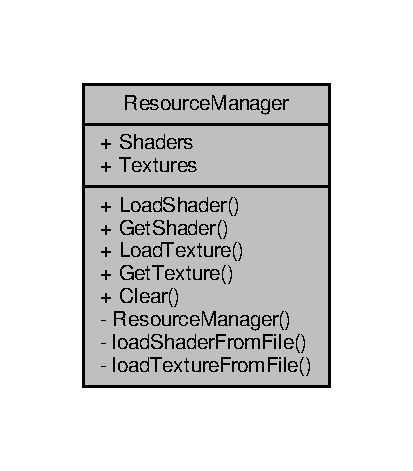
\includegraphics[width=198pt]{classResourceManager__coll__graph}
\end{center}
\end{figure}
\subsection*{Static Public Member Functions}
\begin{DoxyCompactItemize}
\item 
static \hyperlink{classShader}{Shader} $\ast$ \hyperlink{classResourceManager_a241bb97b7dfaf9939fd644ac9fbdd5b4}{Load\+Shader} (const char $\ast$v\+Shader\+File, const char $\ast$f\+Shader\+File, const char $\ast$g\+Shader\+File, std\+::string name)
\item 
static \hyperlink{classShader}{Shader} $\ast$ \hyperlink{classResourceManager_ae95ecdc6de1127616485f7d069437332}{Get\+Shader} (std\+::string name)
\item 
static \hyperlink{classTexture2D}{Texture2D} $\ast$ \hyperlink{classResourceManager_afe6ce47645a38b6e77b838c0edbe0368}{Load\+Texture} (const char $\ast$file, bool alpha, std\+::string name)
\item 
static \hyperlink{classTexture2D}{Texture2D} \& \hyperlink{classResourceManager_a28909ad11a419e76ef00bf6a2b00ac4f}{Get\+Texture} (std\+::string name)
\item 
static void \hyperlink{classResourceManager_aecd08b92634fad3316442c267a04e8c4}{Clear} ()
\end{DoxyCompactItemize}
\subsection*{Static Public Attributes}
\begin{DoxyCompactItemize}
\item 
static std\+::map$<$ std\+::string, \hyperlink{classShader}{Shader} $\ast$ $>$ \hyperlink{classResourceManager_a162a5f89e9ec47ed31692bb1ce76290a}{Shaders}
\item 
static std\+::map$<$ std\+::string, \hyperlink{classTexture2D}{Texture2D} $\ast$ $>$ \hyperlink{classResourceManager_a0a62bc298e457b4b55d185503aa35937}{Textures}
\end{DoxyCompactItemize}
\subsection*{Private Member Functions}
\begin{DoxyCompactItemize}
\item 
\hyperlink{classResourceManager_a3b32babd2e81909bbd90d7f2d566fadb}{Resource\+Manager} ()
\end{DoxyCompactItemize}
\subsection*{Static Private Member Functions}
\begin{DoxyCompactItemize}
\item 
static \hyperlink{classShader}{Shader} $\ast$ \hyperlink{classResourceManager_aeceee147638d827ca8b88a3dba259cb8}{load\+Shader\+From\+File} (const char $\ast$v\+Shader\+File, const char $\ast$f\+Shader\+File, const char $\ast$g\+Shader\+File=nullptr)
\item 
static \hyperlink{classTexture2D}{Texture2D} $\ast$ \hyperlink{classResourceManager_a6fe65aa4de1374cd7f007e564d1c1971}{load\+Texture\+From\+File} (const char $\ast$file, bool alpha)
\end{DoxyCompactItemize}


\subsection{Constructor \& Destructor Documentation}
\mbox{\Hypertarget{classResourceManager_a3b32babd2e81909bbd90d7f2d566fadb}\label{classResourceManager_a3b32babd2e81909bbd90d7f2d566fadb}} 
\index{Resource\+Manager@{Resource\+Manager}!Resource\+Manager@{Resource\+Manager}}
\index{Resource\+Manager@{Resource\+Manager}!Resource\+Manager@{Resource\+Manager}}
\subsubsection{\texorpdfstring{Resource\+Manager()}{ResourceManager()}}
{\footnotesize\ttfamily Resource\+Manager\+::\+Resource\+Manager (\begin{DoxyParamCaption}{ }\end{DoxyParamCaption})\hspace{0.3cm}{\ttfamily [inline]}, {\ttfamily [private]}}



\subsection{Member Function Documentation}
\mbox{\Hypertarget{classResourceManager_aecd08b92634fad3316442c267a04e8c4}\label{classResourceManager_aecd08b92634fad3316442c267a04e8c4}} 
\index{Resource\+Manager@{Resource\+Manager}!Clear@{Clear}}
\index{Clear@{Clear}!Resource\+Manager@{Resource\+Manager}}
\subsubsection{\texorpdfstring{Clear()}{Clear()}}
{\footnotesize\ttfamily void Resource\+Manager\+::\+Clear (\begin{DoxyParamCaption}{ }\end{DoxyParamCaption})\hspace{0.3cm}{\ttfamily [static]}}

\mbox{\Hypertarget{classResourceManager_ae95ecdc6de1127616485f7d069437332}\label{classResourceManager_ae95ecdc6de1127616485f7d069437332}} 
\index{Resource\+Manager@{Resource\+Manager}!Get\+Shader@{Get\+Shader}}
\index{Get\+Shader@{Get\+Shader}!Resource\+Manager@{Resource\+Manager}}
\subsubsection{\texorpdfstring{Get\+Shader()}{GetShader()}}
{\footnotesize\ttfamily \hyperlink{classShader}{Shader} $\ast$ Resource\+Manager\+::\+Get\+Shader (\begin{DoxyParamCaption}\item[{std\+::string}]{name }\end{DoxyParamCaption})\hspace{0.3cm}{\ttfamily [static]}}

\mbox{\Hypertarget{classResourceManager_a28909ad11a419e76ef00bf6a2b00ac4f}\label{classResourceManager_a28909ad11a419e76ef00bf6a2b00ac4f}} 
\index{Resource\+Manager@{Resource\+Manager}!Get\+Texture@{Get\+Texture}}
\index{Get\+Texture@{Get\+Texture}!Resource\+Manager@{Resource\+Manager}}
\subsubsection{\texorpdfstring{Get\+Texture()}{GetTexture()}}
{\footnotesize\ttfamily \hyperlink{classTexture2D}{Texture2D} \& Resource\+Manager\+::\+Get\+Texture (\begin{DoxyParamCaption}\item[{std\+::string}]{name }\end{DoxyParamCaption})\hspace{0.3cm}{\ttfamily [static]}}

\mbox{\Hypertarget{classResourceManager_a241bb97b7dfaf9939fd644ac9fbdd5b4}\label{classResourceManager_a241bb97b7dfaf9939fd644ac9fbdd5b4}} 
\index{Resource\+Manager@{Resource\+Manager}!Load\+Shader@{Load\+Shader}}
\index{Load\+Shader@{Load\+Shader}!Resource\+Manager@{Resource\+Manager}}
\subsubsection{\texorpdfstring{Load\+Shader()}{LoadShader()}}
{\footnotesize\ttfamily \hyperlink{classShader}{Shader} $\ast$ Resource\+Manager\+::\+Load\+Shader (\begin{DoxyParamCaption}\item[{const char $\ast$}]{v\+Shader\+File,  }\item[{const char $\ast$}]{f\+Shader\+File,  }\item[{const char $\ast$}]{g\+Shader\+File,  }\item[{std\+::string}]{name }\end{DoxyParamCaption})\hspace{0.3cm}{\ttfamily [static]}}

\mbox{\Hypertarget{classResourceManager_aeceee147638d827ca8b88a3dba259cb8}\label{classResourceManager_aeceee147638d827ca8b88a3dba259cb8}} 
\index{Resource\+Manager@{Resource\+Manager}!load\+Shader\+From\+File@{load\+Shader\+From\+File}}
\index{load\+Shader\+From\+File@{load\+Shader\+From\+File}!Resource\+Manager@{Resource\+Manager}}
\subsubsection{\texorpdfstring{load\+Shader\+From\+File()}{loadShaderFromFile()}}
{\footnotesize\ttfamily \hyperlink{classShader}{Shader} $\ast$ Resource\+Manager\+::load\+Shader\+From\+File (\begin{DoxyParamCaption}\item[{const char $\ast$}]{v\+Shader\+File,  }\item[{const char $\ast$}]{f\+Shader\+File,  }\item[{const char $\ast$}]{g\+Shader\+File = {\ttfamily nullptr} }\end{DoxyParamCaption})\hspace{0.3cm}{\ttfamily [static]}, {\ttfamily [private]}}

\mbox{\Hypertarget{classResourceManager_afe6ce47645a38b6e77b838c0edbe0368}\label{classResourceManager_afe6ce47645a38b6e77b838c0edbe0368}} 
\index{Resource\+Manager@{Resource\+Manager}!Load\+Texture@{Load\+Texture}}
\index{Load\+Texture@{Load\+Texture}!Resource\+Manager@{Resource\+Manager}}
\subsubsection{\texorpdfstring{Load\+Texture()}{LoadTexture()}}
{\footnotesize\ttfamily \hyperlink{classTexture2D}{Texture2D} $\ast$ Resource\+Manager\+::\+Load\+Texture (\begin{DoxyParamCaption}\item[{const char $\ast$}]{file,  }\item[{bool}]{alpha,  }\item[{std\+::string}]{name }\end{DoxyParamCaption})\hspace{0.3cm}{\ttfamily [static]}}

\mbox{\Hypertarget{classResourceManager_a6fe65aa4de1374cd7f007e564d1c1971}\label{classResourceManager_a6fe65aa4de1374cd7f007e564d1c1971}} 
\index{Resource\+Manager@{Resource\+Manager}!load\+Texture\+From\+File@{load\+Texture\+From\+File}}
\index{load\+Texture\+From\+File@{load\+Texture\+From\+File}!Resource\+Manager@{Resource\+Manager}}
\subsubsection{\texorpdfstring{load\+Texture\+From\+File()}{loadTextureFromFile()}}
{\footnotesize\ttfamily \hyperlink{classTexture2D}{Texture2D} $\ast$ Resource\+Manager\+::load\+Texture\+From\+File (\begin{DoxyParamCaption}\item[{const char $\ast$}]{file,  }\item[{bool}]{alpha }\end{DoxyParamCaption})\hspace{0.3cm}{\ttfamily [static]}, {\ttfamily [private]}}



\subsection{Member Data Documentation}
\mbox{\Hypertarget{classResourceManager_a162a5f89e9ec47ed31692bb1ce76290a}\label{classResourceManager_a162a5f89e9ec47ed31692bb1ce76290a}} 
\index{Resource\+Manager@{Resource\+Manager}!Shaders@{Shaders}}
\index{Shaders@{Shaders}!Resource\+Manager@{Resource\+Manager}}
\subsubsection{\texorpdfstring{Shaders}{Shaders}}
{\footnotesize\ttfamily std\+::map$<$ std\+::string, \hyperlink{classShader}{Shader} $\ast$ $>$ Resource\+Manager\+::\+Shaders\hspace{0.3cm}{\ttfamily [static]}}

\mbox{\Hypertarget{classResourceManager_a0a62bc298e457b4b55d185503aa35937}\label{classResourceManager_a0a62bc298e457b4b55d185503aa35937}} 
\index{Resource\+Manager@{Resource\+Manager}!Textures@{Textures}}
\index{Textures@{Textures}!Resource\+Manager@{Resource\+Manager}}
\subsubsection{\texorpdfstring{Textures}{Textures}}
{\footnotesize\ttfamily std\+::map$<$ std\+::string, \hyperlink{classTexture2D}{Texture2D} $\ast$ $>$ Resource\+Manager\+::\+Textures\hspace{0.3cm}{\ttfamily [static]}}



The documentation for this class was generated from the following files\+:\begin{DoxyCompactItemize}
\item 
/mnt/hdd/\+C0de/smart\+\_\+engine/include/\hyperlink{resource__manager_8h}{resource\+\_\+manager.\+h}\item 
/mnt/hdd/\+C0de/smart\+\_\+engine/src/\hyperlink{resource__manager_8cpp}{resource\+\_\+manager.\+cpp}\end{DoxyCompactItemize}

\hypertarget{classShader}{}\section{Shader Class Reference}
\label{classShader}\index{Shader@{Shader}}


{\ttfamily \#include $<$shader.\+h$>$}



Collaboration diagram for Shader\+:
\nopagebreak
\begin{figure}[H]
\begin{center}
\leavevmode
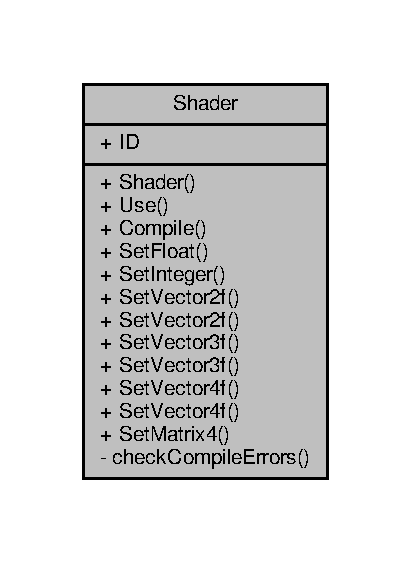
\includegraphics[width=197pt]{classShader__coll__graph}
\end{center}
\end{figure}
\subsection*{Public Member Functions}
\begin{DoxyCompactItemize}
\item 
\hyperlink{classShader_a0d654ebaca4e0555197c0724c6d30610}{Shader} ()
\item 
\hyperlink{classShader}{Shader} \& \hyperlink{classShader_a02292f4fdae284b29169db5da29e519a}{Use} ()
\item 
void \hyperlink{classShader_ace30758935fc09126ec99f5b602cb18f}{Compile} (const char $\ast$vertex\+Source, const char $\ast$fragment\+Source, const char $\ast$geometry\+Source=nullptr)
\item 
void \hyperlink{classShader_a90a74282cd77e51812cd2c0ed0eb5cad}{Set\+Float} (const char $\ast$name, float value, bool use\+Shader=false)
\item 
void \hyperlink{classShader_aac20695848a1a8a283e23d36b0557c20}{Set\+Integer} (const char $\ast$name, int value, bool use\+Shader=false)
\item 
void \hyperlink{classShader_ae5994e58f1eec3278b61655ef2a23b4f}{Set\+Vector2f} (const char $\ast$name, float x, float y, bool use\+Shader=false)
\item 
void \hyperlink{classShader_adf66248417fdee81d48fdd63bbee6805}{Set\+Vector2f} (const char $\ast$name, const glm\+::vec2 \&value, bool use\+Shader=false)
\item 
void \hyperlink{classShader_ac1dbbe3e0134b04c9decf1974252f07b}{Set\+Vector3f} (const char $\ast$name, float x, float y, float z, bool use\+Shader=false)
\item 
void \hyperlink{classShader_a996865767a7485cb63bbd979bb1bc252}{Set\+Vector3f} (const char $\ast$name, const glm\+::vec3 \&value, bool use\+Shader=false)
\item 
void \hyperlink{classShader_a9fd94ef003bab74c968ebde2c9c542b4}{Set\+Vector4f} (const char $\ast$name, float x, float y, float z, float w, bool use\+Shader=false)
\item 
void \hyperlink{classShader_a6bd077475ad23d4eccaf0d4c695c668a}{Set\+Vector4f} (const char $\ast$name, const glm\+::vec4 \&value, bool use\+Shader=false)
\item 
void \hyperlink{classShader_a8bfcef4683f9cba1cfc955b869ee258a}{Set\+Matrix4} (const char $\ast$name, const glm\+::mat4 \&matrix, bool use\+Shader=false)
\end{DoxyCompactItemize}
\subsection*{Public Attributes}
\begin{DoxyCompactItemize}
\item 
unsigned int \hyperlink{classShader_a142a08b6fbdfc982d82ca10ee0b0f38d}{ID}
\end{DoxyCompactItemize}
\subsection*{Private Member Functions}
\begin{DoxyCompactItemize}
\item 
void \hyperlink{classShader_a9ef1a7e7fd62ef1de1a1c1f63dcdef8a}{check\+Compile\+Errors} (unsigned int object, std\+::string type)
\end{DoxyCompactItemize}


\subsection{Constructor \& Destructor Documentation}
\mbox{\Hypertarget{classShader_a0d654ebaca4e0555197c0724c6d30610}\label{classShader_a0d654ebaca4e0555197c0724c6d30610}} 
\index{Shader@{Shader}!Shader@{Shader}}
\index{Shader@{Shader}!Shader@{Shader}}
\subsubsection{\texorpdfstring{Shader()}{Shader()}}
{\footnotesize\ttfamily Shader\+::\+Shader (\begin{DoxyParamCaption}{ }\end{DoxyParamCaption})\hspace{0.3cm}{\ttfamily [inline]}}



\subsection{Member Function Documentation}
\mbox{\Hypertarget{classShader_a9ef1a7e7fd62ef1de1a1c1f63dcdef8a}\label{classShader_a9ef1a7e7fd62ef1de1a1c1f63dcdef8a}} 
\index{Shader@{Shader}!check\+Compile\+Errors@{check\+Compile\+Errors}}
\index{check\+Compile\+Errors@{check\+Compile\+Errors}!Shader@{Shader}}
\subsubsection{\texorpdfstring{check\+Compile\+Errors()}{checkCompileErrors()}}
{\footnotesize\ttfamily void Shader\+::check\+Compile\+Errors (\begin{DoxyParamCaption}\item[{unsigned int}]{object,  }\item[{std\+::string}]{type }\end{DoxyParamCaption})\hspace{0.3cm}{\ttfamily [private]}}

\mbox{\Hypertarget{classShader_ace30758935fc09126ec99f5b602cb18f}\label{classShader_ace30758935fc09126ec99f5b602cb18f}} 
\index{Shader@{Shader}!Compile@{Compile}}
\index{Compile@{Compile}!Shader@{Shader}}
\subsubsection{\texorpdfstring{Compile()}{Compile()}}
{\footnotesize\ttfamily void Shader\+::\+Compile (\begin{DoxyParamCaption}\item[{const char $\ast$}]{vertex\+Source,  }\item[{const char $\ast$}]{fragment\+Source,  }\item[{const char $\ast$}]{geometry\+Source = {\ttfamily nullptr} }\end{DoxyParamCaption})}

\mbox{\Hypertarget{classShader_a90a74282cd77e51812cd2c0ed0eb5cad}\label{classShader_a90a74282cd77e51812cd2c0ed0eb5cad}} 
\index{Shader@{Shader}!Set\+Float@{Set\+Float}}
\index{Set\+Float@{Set\+Float}!Shader@{Shader}}
\subsubsection{\texorpdfstring{Set\+Float()}{SetFloat()}}
{\footnotesize\ttfamily void Shader\+::\+Set\+Float (\begin{DoxyParamCaption}\item[{const char $\ast$}]{name,  }\item[{float}]{value,  }\item[{bool}]{use\+Shader = {\ttfamily false} }\end{DoxyParamCaption})}

\mbox{\Hypertarget{classShader_aac20695848a1a8a283e23d36b0557c20}\label{classShader_aac20695848a1a8a283e23d36b0557c20}} 
\index{Shader@{Shader}!Set\+Integer@{Set\+Integer}}
\index{Set\+Integer@{Set\+Integer}!Shader@{Shader}}
\subsubsection{\texorpdfstring{Set\+Integer()}{SetInteger()}}
{\footnotesize\ttfamily void Shader\+::\+Set\+Integer (\begin{DoxyParamCaption}\item[{const char $\ast$}]{name,  }\item[{int}]{value,  }\item[{bool}]{use\+Shader = {\ttfamily false} }\end{DoxyParamCaption})}

\mbox{\Hypertarget{classShader_a8bfcef4683f9cba1cfc955b869ee258a}\label{classShader_a8bfcef4683f9cba1cfc955b869ee258a}} 
\index{Shader@{Shader}!Set\+Matrix4@{Set\+Matrix4}}
\index{Set\+Matrix4@{Set\+Matrix4}!Shader@{Shader}}
\subsubsection{\texorpdfstring{Set\+Matrix4()}{SetMatrix4()}}
{\footnotesize\ttfamily void Shader\+::\+Set\+Matrix4 (\begin{DoxyParamCaption}\item[{const char $\ast$}]{name,  }\item[{const glm\+::mat4 \&}]{matrix,  }\item[{bool}]{use\+Shader = {\ttfamily false} }\end{DoxyParamCaption})}

\mbox{\Hypertarget{classShader_ae5994e58f1eec3278b61655ef2a23b4f}\label{classShader_ae5994e58f1eec3278b61655ef2a23b4f}} 
\index{Shader@{Shader}!Set\+Vector2f@{Set\+Vector2f}}
\index{Set\+Vector2f@{Set\+Vector2f}!Shader@{Shader}}
\subsubsection{\texorpdfstring{Set\+Vector2f()}{SetVector2f()}\hspace{0.1cm}{\footnotesize\ttfamily [1/2]}}
{\footnotesize\ttfamily void Shader\+::\+Set\+Vector2f (\begin{DoxyParamCaption}\item[{const char $\ast$}]{name,  }\item[{float}]{x,  }\item[{float}]{y,  }\item[{bool}]{use\+Shader = {\ttfamily false} }\end{DoxyParamCaption})}

\mbox{\Hypertarget{classShader_adf66248417fdee81d48fdd63bbee6805}\label{classShader_adf66248417fdee81d48fdd63bbee6805}} 
\index{Shader@{Shader}!Set\+Vector2f@{Set\+Vector2f}}
\index{Set\+Vector2f@{Set\+Vector2f}!Shader@{Shader}}
\subsubsection{\texorpdfstring{Set\+Vector2f()}{SetVector2f()}\hspace{0.1cm}{\footnotesize\ttfamily [2/2]}}
{\footnotesize\ttfamily void Shader\+::\+Set\+Vector2f (\begin{DoxyParamCaption}\item[{const char $\ast$}]{name,  }\item[{const glm\+::vec2 \&}]{value,  }\item[{bool}]{use\+Shader = {\ttfamily false} }\end{DoxyParamCaption})}

\mbox{\Hypertarget{classShader_ac1dbbe3e0134b04c9decf1974252f07b}\label{classShader_ac1dbbe3e0134b04c9decf1974252f07b}} 
\index{Shader@{Shader}!Set\+Vector3f@{Set\+Vector3f}}
\index{Set\+Vector3f@{Set\+Vector3f}!Shader@{Shader}}
\subsubsection{\texorpdfstring{Set\+Vector3f()}{SetVector3f()}\hspace{0.1cm}{\footnotesize\ttfamily [1/2]}}
{\footnotesize\ttfamily void Shader\+::\+Set\+Vector3f (\begin{DoxyParamCaption}\item[{const char $\ast$}]{name,  }\item[{float}]{x,  }\item[{float}]{y,  }\item[{float}]{z,  }\item[{bool}]{use\+Shader = {\ttfamily false} }\end{DoxyParamCaption})}

\mbox{\Hypertarget{classShader_a996865767a7485cb63bbd979bb1bc252}\label{classShader_a996865767a7485cb63bbd979bb1bc252}} 
\index{Shader@{Shader}!Set\+Vector3f@{Set\+Vector3f}}
\index{Set\+Vector3f@{Set\+Vector3f}!Shader@{Shader}}
\subsubsection{\texorpdfstring{Set\+Vector3f()}{SetVector3f()}\hspace{0.1cm}{\footnotesize\ttfamily [2/2]}}
{\footnotesize\ttfamily void Shader\+::\+Set\+Vector3f (\begin{DoxyParamCaption}\item[{const char $\ast$}]{name,  }\item[{const glm\+::vec3 \&}]{value,  }\item[{bool}]{use\+Shader = {\ttfamily false} }\end{DoxyParamCaption})}

\mbox{\Hypertarget{classShader_a9fd94ef003bab74c968ebde2c9c542b4}\label{classShader_a9fd94ef003bab74c968ebde2c9c542b4}} 
\index{Shader@{Shader}!Set\+Vector4f@{Set\+Vector4f}}
\index{Set\+Vector4f@{Set\+Vector4f}!Shader@{Shader}}
\subsubsection{\texorpdfstring{Set\+Vector4f()}{SetVector4f()}\hspace{0.1cm}{\footnotesize\ttfamily [1/2]}}
{\footnotesize\ttfamily void Shader\+::\+Set\+Vector4f (\begin{DoxyParamCaption}\item[{const char $\ast$}]{name,  }\item[{float}]{x,  }\item[{float}]{y,  }\item[{float}]{z,  }\item[{float}]{w,  }\item[{bool}]{use\+Shader = {\ttfamily false} }\end{DoxyParamCaption})}

\mbox{\Hypertarget{classShader_a6bd077475ad23d4eccaf0d4c695c668a}\label{classShader_a6bd077475ad23d4eccaf0d4c695c668a}} 
\index{Shader@{Shader}!Set\+Vector4f@{Set\+Vector4f}}
\index{Set\+Vector4f@{Set\+Vector4f}!Shader@{Shader}}
\subsubsection{\texorpdfstring{Set\+Vector4f()}{SetVector4f()}\hspace{0.1cm}{\footnotesize\ttfamily [2/2]}}
{\footnotesize\ttfamily void Shader\+::\+Set\+Vector4f (\begin{DoxyParamCaption}\item[{const char $\ast$}]{name,  }\item[{const glm\+::vec4 \&}]{value,  }\item[{bool}]{use\+Shader = {\ttfamily false} }\end{DoxyParamCaption})}

\mbox{\Hypertarget{classShader_a02292f4fdae284b29169db5da29e519a}\label{classShader_a02292f4fdae284b29169db5da29e519a}} 
\index{Shader@{Shader}!Use@{Use}}
\index{Use@{Use}!Shader@{Shader}}
\subsubsection{\texorpdfstring{Use()}{Use()}}
{\footnotesize\ttfamily \hyperlink{classShader}{Shader} \& Shader\+::\+Use (\begin{DoxyParamCaption}{ }\end{DoxyParamCaption})}



\subsection{Member Data Documentation}
\mbox{\Hypertarget{classShader_a142a08b6fbdfc982d82ca10ee0b0f38d}\label{classShader_a142a08b6fbdfc982d82ca10ee0b0f38d}} 
\index{Shader@{Shader}!ID@{ID}}
\index{ID@{ID}!Shader@{Shader}}
\subsubsection{\texorpdfstring{ID}{ID}}
{\footnotesize\ttfamily unsigned int Shader\+::\+ID}



The documentation for this class was generated from the following files\+:\begin{DoxyCompactItemize}
\item 
/mnt/hdd/\+C0de/smart\+\_\+engine/include/\hyperlink{shader_8h}{shader.\+h}\item 
/mnt/hdd/\+C0de/smart\+\_\+engine/src/\hyperlink{shader_8cpp}{shader.\+cpp}\end{DoxyCompactItemize}

\hypertarget{classSplashState}{}\section{Splash\+State Class Reference}
\label{classSplashState}\index{Splash\+State@{Splash\+State}}


{\ttfamily \#include $<$splash\+\_\+state.\+h$>$}



Inheritance diagram for Splash\+State\+:
\nopagebreak
\begin{figure}[H]
\begin{center}
\leavevmode
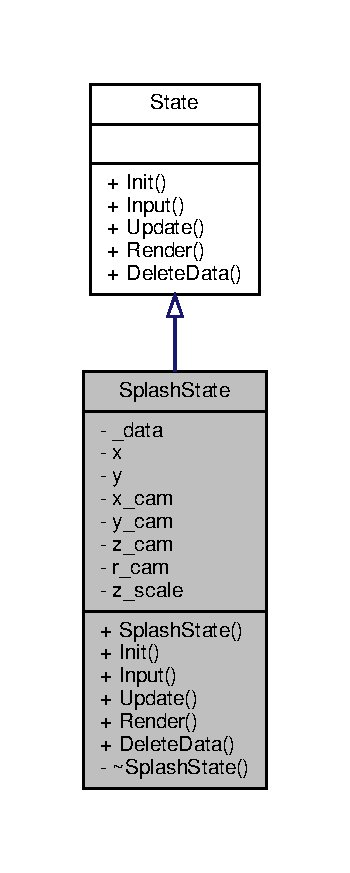
\includegraphics[width=168pt]{classSplashState__inherit__graph}
\end{center}
\end{figure}


Collaboration diagram for Splash\+State\+:
\nopagebreak
\begin{figure}[H]
\begin{center}
\leavevmode
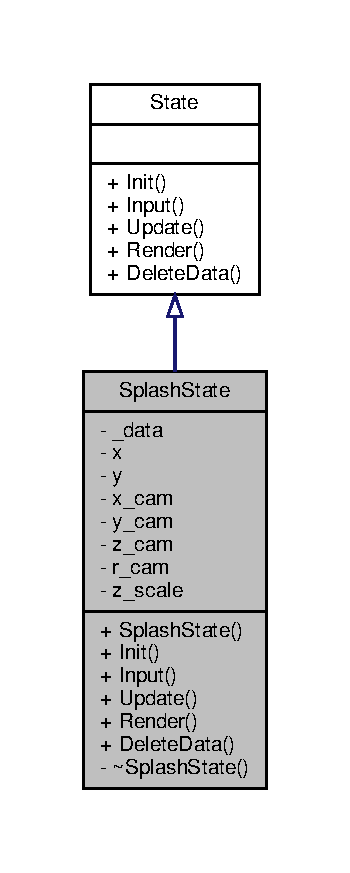
\includegraphics[width=168pt]{classSplashState__coll__graph}
\end{center}
\end{figure}
\subsection*{Public Member Functions}
\begin{DoxyCompactItemize}
\item 
\hyperlink{classSplashState_a4894c4858ae1db288cf9d4f8b03fd2d4}{Splash\+State} (\hyperlink{game_8h_a513c9dd465a0df41dbb4daf40cc717c2}{Game\+Data\+Ref} data)
\item 
void \hyperlink{classSplashState_ae3e0604da087032c179593c237580988}{Init} ()
\item 
void \hyperlink{classSplashState_adb2eb87bd89e41af0c3a9d0903e89450}{Input} (float delta)
\item 
void \hyperlink{classSplashState_af19b293ae1e914e13db4382115e56d2c}{Update} (float delta)
\item 
void \hyperlink{classSplashState_a5efb6f0ede61ec76ee2dd72a6b24c57c}{Render} (float delta)
\item 
void \hyperlink{classSplashState_aca842c8e3ea2642980569ed3b4bb362a}{Delete\+Data} ()
\end{DoxyCompactItemize}
\subsection*{Private Member Functions}
\begin{DoxyCompactItemize}
\item 
\hyperlink{classSplashState_a3171ebc16024564fced18948bf9d7ec5}{$\sim$\+Splash\+State} ()
\end{DoxyCompactItemize}
\subsection*{Private Attributes}
\begin{DoxyCompactItemize}
\item 
\hyperlink{game_8h_a513c9dd465a0df41dbb4daf40cc717c2}{Game\+Data\+Ref} \hyperlink{classSplashState_a45b2f9003eec03f998319695faadfb42}{\+\_\+data}
\item 
float \hyperlink{classSplashState_ad74688dceca650f340e9113938234547}{x}
\item 
float \hyperlink{classSplashState_a4477fcbed7b631aaf135359a09bb0b3c}{y}
\item 
float \hyperlink{classSplashState_a4264ee844097c44c250a95457aa7da2f}{x\+\_\+cam}
\item 
float \hyperlink{classSplashState_adce1ee0219be0b1045a578c4cae88b3b}{y\+\_\+cam}
\item 
float \hyperlink{classSplashState_a4c2362acca2844d0cbcdc2fc958d68a6}{z\+\_\+cam}
\item 
float \hyperlink{classSplashState_a20b119095bf99299609bf381224624c9}{r\+\_\+cam}
\item 
glm\+::vec2 \hyperlink{classSplashState_aa80fb9876f76790eb989071b213c967f}{z\+\_\+scale}
\end{DoxyCompactItemize}


\subsection{Constructor \& Destructor Documentation}
\mbox{\Hypertarget{classSplashState_a4894c4858ae1db288cf9d4f8b03fd2d4}\label{classSplashState_a4894c4858ae1db288cf9d4f8b03fd2d4}} 
\index{Splash\+State@{Splash\+State}!Splash\+State@{Splash\+State}}
\index{Splash\+State@{Splash\+State}!Splash\+State@{Splash\+State}}
\subsubsection{\texorpdfstring{Splash\+State()}{SplashState()}}
{\footnotesize\ttfamily Splash\+State\+::\+Splash\+State (\begin{DoxyParamCaption}\item[{\hyperlink{game_8h_a513c9dd465a0df41dbb4daf40cc717c2}{Game\+Data\+Ref}}]{data }\end{DoxyParamCaption})}

\mbox{\Hypertarget{classSplashState_a3171ebc16024564fced18948bf9d7ec5}\label{classSplashState_a3171ebc16024564fced18948bf9d7ec5}} 
\index{Splash\+State@{Splash\+State}!````~Splash\+State@{$\sim$\+Splash\+State}}
\index{````~Splash\+State@{$\sim$\+Splash\+State}!Splash\+State@{Splash\+State}}
\subsubsection{\texorpdfstring{$\sim$\+Splash\+State()}{~SplashState()}}
{\footnotesize\ttfamily Splash\+State\+::$\sim$\+Splash\+State (\begin{DoxyParamCaption}{ }\end{DoxyParamCaption})\hspace{0.3cm}{\ttfamily [private]}}



\subsection{Member Function Documentation}
\mbox{\Hypertarget{classSplashState_aca842c8e3ea2642980569ed3b4bb362a}\label{classSplashState_aca842c8e3ea2642980569ed3b4bb362a}} 
\index{Splash\+State@{Splash\+State}!Delete\+Data@{Delete\+Data}}
\index{Delete\+Data@{Delete\+Data}!Splash\+State@{Splash\+State}}
\subsubsection{\texorpdfstring{Delete\+Data()}{DeleteData()}}
{\footnotesize\ttfamily void Splash\+State\+::\+Delete\+Data (\begin{DoxyParamCaption}{ }\end{DoxyParamCaption})\hspace{0.3cm}{\ttfamily [virtual]}}



Implements \hyperlink{classState_ade502eaa386d570e526eb356ffd73fd8}{State}.

\mbox{\Hypertarget{classSplashState_ae3e0604da087032c179593c237580988}\label{classSplashState_ae3e0604da087032c179593c237580988}} 
\index{Splash\+State@{Splash\+State}!Init@{Init}}
\index{Init@{Init}!Splash\+State@{Splash\+State}}
\subsubsection{\texorpdfstring{Init()}{Init()}}
{\footnotesize\ttfamily void Splash\+State\+::\+Init (\begin{DoxyParamCaption}{ }\end{DoxyParamCaption})\hspace{0.3cm}{\ttfamily [virtual]}}



Implements \hyperlink{classState_a7ab4d8c6aa239a17ed579d89a209b156}{State}.

\mbox{\Hypertarget{classSplashState_adb2eb87bd89e41af0c3a9d0903e89450}\label{classSplashState_adb2eb87bd89e41af0c3a9d0903e89450}} 
\index{Splash\+State@{Splash\+State}!Input@{Input}}
\index{Input@{Input}!Splash\+State@{Splash\+State}}
\subsubsection{\texorpdfstring{Input()}{Input()}}
{\footnotesize\ttfamily void Splash\+State\+::\+Input (\begin{DoxyParamCaption}\item[{float}]{delta }\end{DoxyParamCaption})\hspace{0.3cm}{\ttfamily [virtual]}}



Implements \hyperlink{classState_a1705412877f37a5cc8fc712542756076}{State}.

\mbox{\Hypertarget{classSplashState_a5efb6f0ede61ec76ee2dd72a6b24c57c}\label{classSplashState_a5efb6f0ede61ec76ee2dd72a6b24c57c}} 
\index{Splash\+State@{Splash\+State}!Render@{Render}}
\index{Render@{Render}!Splash\+State@{Splash\+State}}
\subsubsection{\texorpdfstring{Render()}{Render()}}
{\footnotesize\ttfamily void Splash\+State\+::\+Render (\begin{DoxyParamCaption}\item[{float}]{delta }\end{DoxyParamCaption})\hspace{0.3cm}{\ttfamily [virtual]}}



Implements \hyperlink{classState_a0e48dfae1e3090630475812681417c5f}{State}.

\mbox{\Hypertarget{classSplashState_af19b293ae1e914e13db4382115e56d2c}\label{classSplashState_af19b293ae1e914e13db4382115e56d2c}} 
\index{Splash\+State@{Splash\+State}!Update@{Update}}
\index{Update@{Update}!Splash\+State@{Splash\+State}}
\subsubsection{\texorpdfstring{Update()}{Update()}}
{\footnotesize\ttfamily void Splash\+State\+::\+Update (\begin{DoxyParamCaption}\item[{float}]{delta }\end{DoxyParamCaption})\hspace{0.3cm}{\ttfamily [virtual]}}



Implements \hyperlink{classState_aac0d3fdee1341e168af730b8f31a7bf1}{State}.



\subsection{Member Data Documentation}
\mbox{\Hypertarget{classSplashState_a45b2f9003eec03f998319695faadfb42}\label{classSplashState_a45b2f9003eec03f998319695faadfb42}} 
\index{Splash\+State@{Splash\+State}!\+\_\+data@{\+\_\+data}}
\index{\+\_\+data@{\+\_\+data}!Splash\+State@{Splash\+State}}
\subsubsection{\texorpdfstring{\+\_\+data}{\_data}}
{\footnotesize\ttfamily \hyperlink{game_8h_a513c9dd465a0df41dbb4daf40cc717c2}{Game\+Data\+Ref} Splash\+State\+::\+\_\+data\hspace{0.3cm}{\ttfamily [private]}}

\mbox{\Hypertarget{classSplashState_a20b119095bf99299609bf381224624c9}\label{classSplashState_a20b119095bf99299609bf381224624c9}} 
\index{Splash\+State@{Splash\+State}!r\+\_\+cam@{r\+\_\+cam}}
\index{r\+\_\+cam@{r\+\_\+cam}!Splash\+State@{Splash\+State}}
\subsubsection{\texorpdfstring{r\+\_\+cam}{r\_cam}}
{\footnotesize\ttfamily float Splash\+State\+::r\+\_\+cam\hspace{0.3cm}{\ttfamily [private]}}

\mbox{\Hypertarget{classSplashState_ad74688dceca650f340e9113938234547}\label{classSplashState_ad74688dceca650f340e9113938234547}} 
\index{Splash\+State@{Splash\+State}!x@{x}}
\index{x@{x}!Splash\+State@{Splash\+State}}
\subsubsection{\texorpdfstring{x}{x}}
{\footnotesize\ttfamily float Splash\+State\+::x\hspace{0.3cm}{\ttfamily [private]}}

\mbox{\Hypertarget{classSplashState_a4264ee844097c44c250a95457aa7da2f}\label{classSplashState_a4264ee844097c44c250a95457aa7da2f}} 
\index{Splash\+State@{Splash\+State}!x\+\_\+cam@{x\+\_\+cam}}
\index{x\+\_\+cam@{x\+\_\+cam}!Splash\+State@{Splash\+State}}
\subsubsection{\texorpdfstring{x\+\_\+cam}{x\_cam}}
{\footnotesize\ttfamily float Splash\+State\+::x\+\_\+cam\hspace{0.3cm}{\ttfamily [private]}}

\mbox{\Hypertarget{classSplashState_a4477fcbed7b631aaf135359a09bb0b3c}\label{classSplashState_a4477fcbed7b631aaf135359a09bb0b3c}} 
\index{Splash\+State@{Splash\+State}!y@{y}}
\index{y@{y}!Splash\+State@{Splash\+State}}
\subsubsection{\texorpdfstring{y}{y}}
{\footnotesize\ttfamily float Splash\+State\+::y\hspace{0.3cm}{\ttfamily [private]}}

\mbox{\Hypertarget{classSplashState_adce1ee0219be0b1045a578c4cae88b3b}\label{classSplashState_adce1ee0219be0b1045a578c4cae88b3b}} 
\index{Splash\+State@{Splash\+State}!y\+\_\+cam@{y\+\_\+cam}}
\index{y\+\_\+cam@{y\+\_\+cam}!Splash\+State@{Splash\+State}}
\subsubsection{\texorpdfstring{y\+\_\+cam}{y\_cam}}
{\footnotesize\ttfamily float Splash\+State\+::y\+\_\+cam\hspace{0.3cm}{\ttfamily [private]}}

\mbox{\Hypertarget{classSplashState_a4c2362acca2844d0cbcdc2fc958d68a6}\label{classSplashState_a4c2362acca2844d0cbcdc2fc958d68a6}} 
\index{Splash\+State@{Splash\+State}!z\+\_\+cam@{z\+\_\+cam}}
\index{z\+\_\+cam@{z\+\_\+cam}!Splash\+State@{Splash\+State}}
\subsubsection{\texorpdfstring{z\+\_\+cam}{z\_cam}}
{\footnotesize\ttfamily float Splash\+State\+::z\+\_\+cam\hspace{0.3cm}{\ttfamily [private]}}

\mbox{\Hypertarget{classSplashState_aa80fb9876f76790eb989071b213c967f}\label{classSplashState_aa80fb9876f76790eb989071b213c967f}} 
\index{Splash\+State@{Splash\+State}!z\+\_\+scale@{z\+\_\+scale}}
\index{z\+\_\+scale@{z\+\_\+scale}!Splash\+State@{Splash\+State}}
\subsubsection{\texorpdfstring{z\+\_\+scale}{z\_scale}}
{\footnotesize\ttfamily glm\+::vec2 Splash\+State\+::z\+\_\+scale\hspace{0.3cm}{\ttfamily [private]}}



The documentation for this class was generated from the following files\+:\begin{DoxyCompactItemize}
\item 
/mnt/hdd/\+C0de/smart\+\_\+engine/include/\hyperlink{splash__state_8h}{splash\+\_\+state.\+h}\item 
/mnt/hdd/\+C0de/smart\+\_\+engine/src/\hyperlink{splash__state_8cpp}{splash\+\_\+state.\+cpp}\end{DoxyCompactItemize}

\hypertarget{classsprite}{}\section{sprite Class Reference}
\label{classsprite}\index{sprite@{sprite}}


{\ttfamily \#include $<$sprite.\+h$>$}



Collaboration diagram for sprite\+:
\nopagebreak
\begin{figure}[H]
\begin{center}
\leavevmode
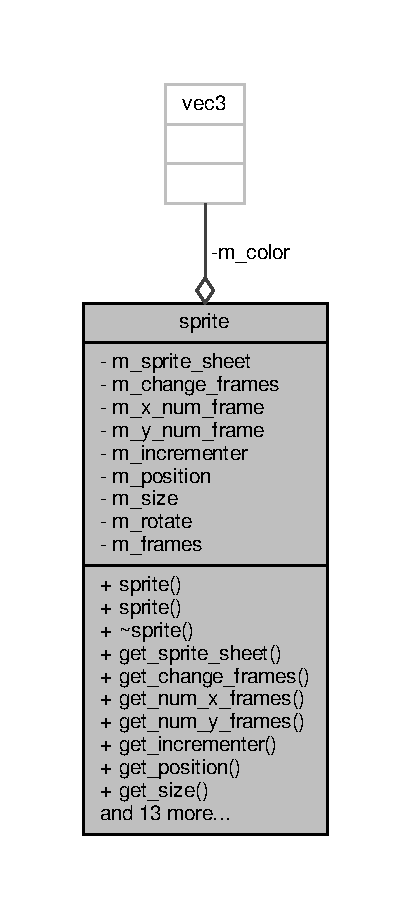
\includegraphics[width=197pt]{classsprite__coll__graph}
\end{center}
\end{figure}
\subsection*{Public Member Functions}
\begin{DoxyCompactItemize}
\item 
\hyperlink{classsprite_ab301a52437b1fedba953a3a3003d3a0d}{sprite} ()
\item 
\hyperlink{classsprite_a16fd4fd92c1244afa585c3b6ef3994ca}{sprite} (bool, bool, unsigned int x\+\_\+frame, unsigned int y\+\_\+frame, float inc, glm\+::vec2, glm\+::vec2, float, glm\+::vec3, glm\+::vec2)
\item 
\hyperlink{classsprite_aa2c57852113368003657c673e39b6f3a}{$\sim$sprite} ()
\item 
bool \hyperlink{classsprite_a6b2f3ae0858b040330d66a547543d91e}{get\+\_\+sprite\+\_\+sheet} ()
\item 
bool \hyperlink{classsprite_a935dcb319f155f0fcb698e2c082e3f2c}{get\+\_\+change\+\_\+frames} ()
\item 
unsigned int \hyperlink{classsprite_aebcc7d599cc15c0257382d23ec5cf4c0}{get\+\_\+num\+\_\+x\+\_\+frames} ()
\item 
unsigned int \hyperlink{classsprite_abc1ab26e93ef1343ca030a14a8b4d250}{get\+\_\+num\+\_\+y\+\_\+frames} ()
\item 
float \hyperlink{classsprite_a34d638c04ee20e0640b121432a9b2bc2}{get\+\_\+incrementer} ()
\item 
glm\+::vec2 \hyperlink{classsprite_a07206378cd6008b2652906d348a0ea7c}{get\+\_\+position} ()
\item 
glm\+::vec2 \hyperlink{classsprite_afe4f7c1f28277a1942cf5f5bb5058fde}{get\+\_\+size} ()
\item 
float \hyperlink{classsprite_a7b6bbbb227a4558c7d4a0e8fc4344bca}{get\+\_\+rotation} ()
\item 
glm\+::vec3 \hyperlink{classsprite_a22a4f69358c9184a54173296d965db32}{get\+\_\+color} ()
\item 
glm\+::vec2 \hyperlink{classsprite_abf33f325e9a1dc0b7b7ff6a26fca4ba4}{get\+\_\+frame} ()
\item 
void \hyperlink{classsprite_aba784f0507715f2e5a9c9eec4c84c868}{set\+\_\+sprite\+\_\+sheet} (bool sprite\+\_\+sheet)
\item 
void \hyperlink{classsprite_ab682d38f77706a999f53a1e62bf2539e}{set\+\_\+change\+\_\+frames} (bool change\+\_\+frames)
\item 
void \hyperlink{classsprite_a87addb8ca942a7654005e2ac51ce2659}{set\+\_\+num\+\_\+x\+\_\+frames} (unsigned int num\+\_\+x\+\_\+frames)
\item 
void \hyperlink{classsprite_a46329102a20cd83a62a2273a78155ac6}{set\+\_\+num\+\_\+y\+\_\+frames} (unsigned int num\+\_\+y\+\_\+frames)
\item 
void \hyperlink{classsprite_ae3c9856eee554bf235ea32433a9cda60}{set\+\_\+incrementer} (float incrementer)
\item 
void \hyperlink{classsprite_aa1d4e098048948fe81239c01365a0656}{set\+\_\+position} (glm\+::vec2 position)
\item 
void \hyperlink{classsprite_a61c40faac76e6c0a5834c34c55f0e4c4}{set\+\_\+size} (glm\+::vec2 size)
\item 
void \hyperlink{classsprite_ab95aac27f21039f0f8584343687e734b}{set\+\_\+rotation} (float rotation)
\item 
void \hyperlink{classsprite_ad9ead060273297a219478f570e17e399}{set\+\_\+color} (glm\+::vec3 color)
\item 
void \hyperlink{classsprite_aeaf9e60fb358bf55a1dd9be38e841ea5}{set\+\_\+frames} (glm\+::vec2 frame)
\end{DoxyCompactItemize}
\subsection*{Private Attributes}
\begin{DoxyCompactItemize}
\item 
bool \hyperlink{classsprite_a90713ede82ab2256a308feae3ec5e3eb}{m\+\_\+sprite\+\_\+sheet}
\item 
bool \hyperlink{classsprite_a29b0927a7303c9156b9caf753501db06}{m\+\_\+change\+\_\+frames}
\item 
unsigned int \hyperlink{classsprite_a8d67c4d9227e4013248b17a702504660}{m\+\_\+x\+\_\+num\+\_\+frame}
\item 
unsigned int \hyperlink{classsprite_a7322a7d73bc48184721ce0d239aaa586}{m\+\_\+y\+\_\+num\+\_\+frame}
\item 
float \hyperlink{classsprite_aecbf0a0cd9ea195f174be3aaa921f057}{m\+\_\+incrementer}
\item 
glm\+::vec2 \hyperlink{classsprite_ad0672bebb7a8202d38b4e6b6ac940f0a}{m\+\_\+position}
\item 
glm\+::vec2 \hyperlink{classsprite_a8935cb487f4f6990d0dad69074c33c7f}{m\+\_\+size}
\item 
float \hyperlink{classsprite_a0d9b789deca4f552207112656ef62363}{m\+\_\+rotate}
\item 
glm\+::vec3 \hyperlink{classsprite_a4c008267c43c6bafcbc0dd3349d4b1da}{m\+\_\+color}
\item 
glm\+::vec2 \hyperlink{classsprite_af81112db3137186237f617a685498c69}{m\+\_\+frames}
\end{DoxyCompactItemize}


\subsection{Constructor \& Destructor Documentation}
\mbox{\Hypertarget{classsprite_ab301a52437b1fedba953a3a3003d3a0d}\label{classsprite_ab301a52437b1fedba953a3a3003d3a0d}} 
\index{sprite@{sprite}!sprite@{sprite}}
\index{sprite@{sprite}!sprite@{sprite}}
\subsubsection{\texorpdfstring{sprite()}{sprite()}\hspace{0.1cm}{\footnotesize\ttfamily [1/2]}}
{\footnotesize\ttfamily sprite\+::sprite (\begin{DoxyParamCaption}{ }\end{DoxyParamCaption})\hspace{0.3cm}{\ttfamily [inline]}}

\mbox{\Hypertarget{classsprite_a16fd4fd92c1244afa585c3b6ef3994ca}\label{classsprite_a16fd4fd92c1244afa585c3b6ef3994ca}} 
\index{sprite@{sprite}!sprite@{sprite}}
\index{sprite@{sprite}!sprite@{sprite}}
\subsubsection{\texorpdfstring{sprite()}{sprite()}\hspace{0.1cm}{\footnotesize\ttfamily [2/2]}}
{\footnotesize\ttfamily sprite\+::sprite (\begin{DoxyParamCaption}\item[{bool}]{sprite\+\_\+sheet,  }\item[{bool}]{change\+\_\+frames,  }\item[{unsigned int}]{x\+\_\+frame,  }\item[{unsigned int}]{y\+\_\+frame,  }\item[{float}]{inc,  }\item[{glm\+::vec2}]{position,  }\item[{glm\+::vec2}]{size,  }\item[{float}]{rotation,  }\item[{glm\+::vec3}]{color,  }\item[{glm\+::vec2}]{frames }\end{DoxyParamCaption})}

\mbox{\Hypertarget{classsprite_aa2c57852113368003657c673e39b6f3a}\label{classsprite_aa2c57852113368003657c673e39b6f3a}} 
\index{sprite@{sprite}!````~sprite@{$\sim$sprite}}
\index{````~sprite@{$\sim$sprite}!sprite@{sprite}}
\subsubsection{\texorpdfstring{$\sim$sprite()}{~sprite()}}
{\footnotesize\ttfamily sprite\+::$\sim$sprite (\begin{DoxyParamCaption}{ }\end{DoxyParamCaption})\hspace{0.3cm}{\ttfamily [inline]}}



\subsection{Member Function Documentation}
\mbox{\Hypertarget{classsprite_a935dcb319f155f0fcb698e2c082e3f2c}\label{classsprite_a935dcb319f155f0fcb698e2c082e3f2c}} 
\index{sprite@{sprite}!get\+\_\+change\+\_\+frames@{get\+\_\+change\+\_\+frames}}
\index{get\+\_\+change\+\_\+frames@{get\+\_\+change\+\_\+frames}!sprite@{sprite}}
\subsubsection{\texorpdfstring{get\+\_\+change\+\_\+frames()}{get\_change\_frames()}}
{\footnotesize\ttfamily bool sprite\+::get\+\_\+change\+\_\+frames (\begin{DoxyParamCaption}{ }\end{DoxyParamCaption})\hspace{0.3cm}{\ttfamily [inline]}}

\mbox{\Hypertarget{classsprite_a22a4f69358c9184a54173296d965db32}\label{classsprite_a22a4f69358c9184a54173296d965db32}} 
\index{sprite@{sprite}!get\+\_\+color@{get\+\_\+color}}
\index{get\+\_\+color@{get\+\_\+color}!sprite@{sprite}}
\subsubsection{\texorpdfstring{get\+\_\+color()}{get\_color()}}
{\footnotesize\ttfamily glm\+::vec3 sprite\+::get\+\_\+color (\begin{DoxyParamCaption}{ }\end{DoxyParamCaption})\hspace{0.3cm}{\ttfamily [inline]}}

\mbox{\Hypertarget{classsprite_abf33f325e9a1dc0b7b7ff6a26fca4ba4}\label{classsprite_abf33f325e9a1dc0b7b7ff6a26fca4ba4}} 
\index{sprite@{sprite}!get\+\_\+frame@{get\+\_\+frame}}
\index{get\+\_\+frame@{get\+\_\+frame}!sprite@{sprite}}
\subsubsection{\texorpdfstring{get\+\_\+frame()}{get\_frame()}}
{\footnotesize\ttfamily glm\+::vec2 sprite\+::get\+\_\+frame (\begin{DoxyParamCaption}{ }\end{DoxyParamCaption})\hspace{0.3cm}{\ttfamily [inline]}}

\mbox{\Hypertarget{classsprite_a34d638c04ee20e0640b121432a9b2bc2}\label{classsprite_a34d638c04ee20e0640b121432a9b2bc2}} 
\index{sprite@{sprite}!get\+\_\+incrementer@{get\+\_\+incrementer}}
\index{get\+\_\+incrementer@{get\+\_\+incrementer}!sprite@{sprite}}
\subsubsection{\texorpdfstring{get\+\_\+incrementer()}{get\_incrementer()}}
{\footnotesize\ttfamily float sprite\+::get\+\_\+incrementer (\begin{DoxyParamCaption}{ }\end{DoxyParamCaption})\hspace{0.3cm}{\ttfamily [inline]}}

\mbox{\Hypertarget{classsprite_aebcc7d599cc15c0257382d23ec5cf4c0}\label{classsprite_aebcc7d599cc15c0257382d23ec5cf4c0}} 
\index{sprite@{sprite}!get\+\_\+num\+\_\+x\+\_\+frames@{get\+\_\+num\+\_\+x\+\_\+frames}}
\index{get\+\_\+num\+\_\+x\+\_\+frames@{get\+\_\+num\+\_\+x\+\_\+frames}!sprite@{sprite}}
\subsubsection{\texorpdfstring{get\+\_\+num\+\_\+x\+\_\+frames()}{get\_num\_x\_frames()}}
{\footnotesize\ttfamily unsigned int sprite\+::get\+\_\+num\+\_\+x\+\_\+frames (\begin{DoxyParamCaption}{ }\end{DoxyParamCaption})\hspace{0.3cm}{\ttfamily [inline]}}

\mbox{\Hypertarget{classsprite_abc1ab26e93ef1343ca030a14a8b4d250}\label{classsprite_abc1ab26e93ef1343ca030a14a8b4d250}} 
\index{sprite@{sprite}!get\+\_\+num\+\_\+y\+\_\+frames@{get\+\_\+num\+\_\+y\+\_\+frames}}
\index{get\+\_\+num\+\_\+y\+\_\+frames@{get\+\_\+num\+\_\+y\+\_\+frames}!sprite@{sprite}}
\subsubsection{\texorpdfstring{get\+\_\+num\+\_\+y\+\_\+frames()}{get\_num\_y\_frames()}}
{\footnotesize\ttfamily unsigned int sprite\+::get\+\_\+num\+\_\+y\+\_\+frames (\begin{DoxyParamCaption}{ }\end{DoxyParamCaption})\hspace{0.3cm}{\ttfamily [inline]}}

\mbox{\Hypertarget{classsprite_a07206378cd6008b2652906d348a0ea7c}\label{classsprite_a07206378cd6008b2652906d348a0ea7c}} 
\index{sprite@{sprite}!get\+\_\+position@{get\+\_\+position}}
\index{get\+\_\+position@{get\+\_\+position}!sprite@{sprite}}
\subsubsection{\texorpdfstring{get\+\_\+position()}{get\_position()}}
{\footnotesize\ttfamily glm\+::vec2 sprite\+::get\+\_\+position (\begin{DoxyParamCaption}{ }\end{DoxyParamCaption})\hspace{0.3cm}{\ttfamily [inline]}}

\mbox{\Hypertarget{classsprite_a7b6bbbb227a4558c7d4a0e8fc4344bca}\label{classsprite_a7b6bbbb227a4558c7d4a0e8fc4344bca}} 
\index{sprite@{sprite}!get\+\_\+rotation@{get\+\_\+rotation}}
\index{get\+\_\+rotation@{get\+\_\+rotation}!sprite@{sprite}}
\subsubsection{\texorpdfstring{get\+\_\+rotation()}{get\_rotation()}}
{\footnotesize\ttfamily float sprite\+::get\+\_\+rotation (\begin{DoxyParamCaption}{ }\end{DoxyParamCaption})\hspace{0.3cm}{\ttfamily [inline]}}

\mbox{\Hypertarget{classsprite_afe4f7c1f28277a1942cf5f5bb5058fde}\label{classsprite_afe4f7c1f28277a1942cf5f5bb5058fde}} 
\index{sprite@{sprite}!get\+\_\+size@{get\+\_\+size}}
\index{get\+\_\+size@{get\+\_\+size}!sprite@{sprite}}
\subsubsection{\texorpdfstring{get\+\_\+size()}{get\_size()}}
{\footnotesize\ttfamily glm\+::vec2 sprite\+::get\+\_\+size (\begin{DoxyParamCaption}{ }\end{DoxyParamCaption})\hspace{0.3cm}{\ttfamily [inline]}}

\mbox{\Hypertarget{classsprite_a6b2f3ae0858b040330d66a547543d91e}\label{classsprite_a6b2f3ae0858b040330d66a547543d91e}} 
\index{sprite@{sprite}!get\+\_\+sprite\+\_\+sheet@{get\+\_\+sprite\+\_\+sheet}}
\index{get\+\_\+sprite\+\_\+sheet@{get\+\_\+sprite\+\_\+sheet}!sprite@{sprite}}
\subsubsection{\texorpdfstring{get\+\_\+sprite\+\_\+sheet()}{get\_sprite\_sheet()}}
{\footnotesize\ttfamily bool sprite\+::get\+\_\+sprite\+\_\+sheet (\begin{DoxyParamCaption}{ }\end{DoxyParamCaption})\hspace{0.3cm}{\ttfamily [inline]}}

\mbox{\Hypertarget{classsprite_ab682d38f77706a999f53a1e62bf2539e}\label{classsprite_ab682d38f77706a999f53a1e62bf2539e}} 
\index{sprite@{sprite}!set\+\_\+change\+\_\+frames@{set\+\_\+change\+\_\+frames}}
\index{set\+\_\+change\+\_\+frames@{set\+\_\+change\+\_\+frames}!sprite@{sprite}}
\subsubsection{\texorpdfstring{set\+\_\+change\+\_\+frames()}{set\_change\_frames()}}
{\footnotesize\ttfamily void sprite\+::set\+\_\+change\+\_\+frames (\begin{DoxyParamCaption}\item[{bool}]{change\+\_\+frames }\end{DoxyParamCaption})\hspace{0.3cm}{\ttfamily [inline]}}

\mbox{\Hypertarget{classsprite_ad9ead060273297a219478f570e17e399}\label{classsprite_ad9ead060273297a219478f570e17e399}} 
\index{sprite@{sprite}!set\+\_\+color@{set\+\_\+color}}
\index{set\+\_\+color@{set\+\_\+color}!sprite@{sprite}}
\subsubsection{\texorpdfstring{set\+\_\+color()}{set\_color()}}
{\footnotesize\ttfamily void sprite\+::set\+\_\+color (\begin{DoxyParamCaption}\item[{glm\+::vec3}]{color }\end{DoxyParamCaption})\hspace{0.3cm}{\ttfamily [inline]}}

\mbox{\Hypertarget{classsprite_aeaf9e60fb358bf55a1dd9be38e841ea5}\label{classsprite_aeaf9e60fb358bf55a1dd9be38e841ea5}} 
\index{sprite@{sprite}!set\+\_\+frames@{set\+\_\+frames}}
\index{set\+\_\+frames@{set\+\_\+frames}!sprite@{sprite}}
\subsubsection{\texorpdfstring{set\+\_\+frames()}{set\_frames()}}
{\footnotesize\ttfamily void sprite\+::set\+\_\+frames (\begin{DoxyParamCaption}\item[{glm\+::vec2}]{frame }\end{DoxyParamCaption})\hspace{0.3cm}{\ttfamily [inline]}}

\mbox{\Hypertarget{classsprite_ae3c9856eee554bf235ea32433a9cda60}\label{classsprite_ae3c9856eee554bf235ea32433a9cda60}} 
\index{sprite@{sprite}!set\+\_\+incrementer@{set\+\_\+incrementer}}
\index{set\+\_\+incrementer@{set\+\_\+incrementer}!sprite@{sprite}}
\subsubsection{\texorpdfstring{set\+\_\+incrementer()}{set\_incrementer()}}
{\footnotesize\ttfamily void sprite\+::set\+\_\+incrementer (\begin{DoxyParamCaption}\item[{float}]{incrementer }\end{DoxyParamCaption})\hspace{0.3cm}{\ttfamily [inline]}}

\mbox{\Hypertarget{classsprite_a87addb8ca942a7654005e2ac51ce2659}\label{classsprite_a87addb8ca942a7654005e2ac51ce2659}} 
\index{sprite@{sprite}!set\+\_\+num\+\_\+x\+\_\+frames@{set\+\_\+num\+\_\+x\+\_\+frames}}
\index{set\+\_\+num\+\_\+x\+\_\+frames@{set\+\_\+num\+\_\+x\+\_\+frames}!sprite@{sprite}}
\subsubsection{\texorpdfstring{set\+\_\+num\+\_\+x\+\_\+frames()}{set\_num\_x\_frames()}}
{\footnotesize\ttfamily void sprite\+::set\+\_\+num\+\_\+x\+\_\+frames (\begin{DoxyParamCaption}\item[{unsigned int}]{num\+\_\+x\+\_\+frames }\end{DoxyParamCaption})\hspace{0.3cm}{\ttfamily [inline]}}

\mbox{\Hypertarget{classsprite_a46329102a20cd83a62a2273a78155ac6}\label{classsprite_a46329102a20cd83a62a2273a78155ac6}} 
\index{sprite@{sprite}!set\+\_\+num\+\_\+y\+\_\+frames@{set\+\_\+num\+\_\+y\+\_\+frames}}
\index{set\+\_\+num\+\_\+y\+\_\+frames@{set\+\_\+num\+\_\+y\+\_\+frames}!sprite@{sprite}}
\subsubsection{\texorpdfstring{set\+\_\+num\+\_\+y\+\_\+frames()}{set\_num\_y\_frames()}}
{\footnotesize\ttfamily void sprite\+::set\+\_\+num\+\_\+y\+\_\+frames (\begin{DoxyParamCaption}\item[{unsigned int}]{num\+\_\+y\+\_\+frames }\end{DoxyParamCaption})\hspace{0.3cm}{\ttfamily [inline]}}

\mbox{\Hypertarget{classsprite_aa1d4e098048948fe81239c01365a0656}\label{classsprite_aa1d4e098048948fe81239c01365a0656}} 
\index{sprite@{sprite}!set\+\_\+position@{set\+\_\+position}}
\index{set\+\_\+position@{set\+\_\+position}!sprite@{sprite}}
\subsubsection{\texorpdfstring{set\+\_\+position()}{set\_position()}}
{\footnotesize\ttfamily void sprite\+::set\+\_\+position (\begin{DoxyParamCaption}\item[{glm\+::vec2}]{position }\end{DoxyParamCaption})\hspace{0.3cm}{\ttfamily [inline]}}

\mbox{\Hypertarget{classsprite_ab95aac27f21039f0f8584343687e734b}\label{classsprite_ab95aac27f21039f0f8584343687e734b}} 
\index{sprite@{sprite}!set\+\_\+rotation@{set\+\_\+rotation}}
\index{set\+\_\+rotation@{set\+\_\+rotation}!sprite@{sprite}}
\subsubsection{\texorpdfstring{set\+\_\+rotation()}{set\_rotation()}}
{\footnotesize\ttfamily void sprite\+::set\+\_\+rotation (\begin{DoxyParamCaption}\item[{float}]{rotation }\end{DoxyParamCaption})\hspace{0.3cm}{\ttfamily [inline]}}

\mbox{\Hypertarget{classsprite_a61c40faac76e6c0a5834c34c55f0e4c4}\label{classsprite_a61c40faac76e6c0a5834c34c55f0e4c4}} 
\index{sprite@{sprite}!set\+\_\+size@{set\+\_\+size}}
\index{set\+\_\+size@{set\+\_\+size}!sprite@{sprite}}
\subsubsection{\texorpdfstring{set\+\_\+size()}{set\_size()}}
{\footnotesize\ttfamily void sprite\+::set\+\_\+size (\begin{DoxyParamCaption}\item[{glm\+::vec2}]{size }\end{DoxyParamCaption})\hspace{0.3cm}{\ttfamily [inline]}}

\mbox{\Hypertarget{classsprite_aba784f0507715f2e5a9c9eec4c84c868}\label{classsprite_aba784f0507715f2e5a9c9eec4c84c868}} 
\index{sprite@{sprite}!set\+\_\+sprite\+\_\+sheet@{set\+\_\+sprite\+\_\+sheet}}
\index{set\+\_\+sprite\+\_\+sheet@{set\+\_\+sprite\+\_\+sheet}!sprite@{sprite}}
\subsubsection{\texorpdfstring{set\+\_\+sprite\+\_\+sheet()}{set\_sprite\_sheet()}}
{\footnotesize\ttfamily void sprite\+::set\+\_\+sprite\+\_\+sheet (\begin{DoxyParamCaption}\item[{bool}]{sprite\+\_\+sheet }\end{DoxyParamCaption})\hspace{0.3cm}{\ttfamily [inline]}}



\subsection{Member Data Documentation}
\mbox{\Hypertarget{classsprite_a29b0927a7303c9156b9caf753501db06}\label{classsprite_a29b0927a7303c9156b9caf753501db06}} 
\index{sprite@{sprite}!m\+\_\+change\+\_\+frames@{m\+\_\+change\+\_\+frames}}
\index{m\+\_\+change\+\_\+frames@{m\+\_\+change\+\_\+frames}!sprite@{sprite}}
\subsubsection{\texorpdfstring{m\+\_\+change\+\_\+frames}{m\_change\_frames}}
{\footnotesize\ttfamily bool sprite\+::m\+\_\+change\+\_\+frames\hspace{0.3cm}{\ttfamily [private]}}

\mbox{\Hypertarget{classsprite_a4c008267c43c6bafcbc0dd3349d4b1da}\label{classsprite_a4c008267c43c6bafcbc0dd3349d4b1da}} 
\index{sprite@{sprite}!m\+\_\+color@{m\+\_\+color}}
\index{m\+\_\+color@{m\+\_\+color}!sprite@{sprite}}
\subsubsection{\texorpdfstring{m\+\_\+color}{m\_color}}
{\footnotesize\ttfamily glm\+::vec3 sprite\+::m\+\_\+color\hspace{0.3cm}{\ttfamily [private]}}

\mbox{\Hypertarget{classsprite_af81112db3137186237f617a685498c69}\label{classsprite_af81112db3137186237f617a685498c69}} 
\index{sprite@{sprite}!m\+\_\+frames@{m\+\_\+frames}}
\index{m\+\_\+frames@{m\+\_\+frames}!sprite@{sprite}}
\subsubsection{\texorpdfstring{m\+\_\+frames}{m\_frames}}
{\footnotesize\ttfamily glm\+::vec2 sprite\+::m\+\_\+frames\hspace{0.3cm}{\ttfamily [private]}}

\mbox{\Hypertarget{classsprite_aecbf0a0cd9ea195f174be3aaa921f057}\label{classsprite_aecbf0a0cd9ea195f174be3aaa921f057}} 
\index{sprite@{sprite}!m\+\_\+incrementer@{m\+\_\+incrementer}}
\index{m\+\_\+incrementer@{m\+\_\+incrementer}!sprite@{sprite}}
\subsubsection{\texorpdfstring{m\+\_\+incrementer}{m\_incrementer}}
{\footnotesize\ttfamily float sprite\+::m\+\_\+incrementer\hspace{0.3cm}{\ttfamily [private]}}

\mbox{\Hypertarget{classsprite_ad0672bebb7a8202d38b4e6b6ac940f0a}\label{classsprite_ad0672bebb7a8202d38b4e6b6ac940f0a}} 
\index{sprite@{sprite}!m\+\_\+position@{m\+\_\+position}}
\index{m\+\_\+position@{m\+\_\+position}!sprite@{sprite}}
\subsubsection{\texorpdfstring{m\+\_\+position}{m\_position}}
{\footnotesize\ttfamily glm\+::vec2 sprite\+::m\+\_\+position\hspace{0.3cm}{\ttfamily [private]}}

\mbox{\Hypertarget{classsprite_a0d9b789deca4f552207112656ef62363}\label{classsprite_a0d9b789deca4f552207112656ef62363}} 
\index{sprite@{sprite}!m\+\_\+rotate@{m\+\_\+rotate}}
\index{m\+\_\+rotate@{m\+\_\+rotate}!sprite@{sprite}}
\subsubsection{\texorpdfstring{m\+\_\+rotate}{m\_rotate}}
{\footnotesize\ttfamily float sprite\+::m\+\_\+rotate\hspace{0.3cm}{\ttfamily [private]}}

\mbox{\Hypertarget{classsprite_a8935cb487f4f6990d0dad69074c33c7f}\label{classsprite_a8935cb487f4f6990d0dad69074c33c7f}} 
\index{sprite@{sprite}!m\+\_\+size@{m\+\_\+size}}
\index{m\+\_\+size@{m\+\_\+size}!sprite@{sprite}}
\subsubsection{\texorpdfstring{m\+\_\+size}{m\_size}}
{\footnotesize\ttfamily glm\+::vec2 sprite\+::m\+\_\+size\hspace{0.3cm}{\ttfamily [private]}}

\mbox{\Hypertarget{classsprite_a90713ede82ab2256a308feae3ec5e3eb}\label{classsprite_a90713ede82ab2256a308feae3ec5e3eb}} 
\index{sprite@{sprite}!m\+\_\+sprite\+\_\+sheet@{m\+\_\+sprite\+\_\+sheet}}
\index{m\+\_\+sprite\+\_\+sheet@{m\+\_\+sprite\+\_\+sheet}!sprite@{sprite}}
\subsubsection{\texorpdfstring{m\+\_\+sprite\+\_\+sheet}{m\_sprite\_sheet}}
{\footnotesize\ttfamily bool sprite\+::m\+\_\+sprite\+\_\+sheet\hspace{0.3cm}{\ttfamily [private]}}

\mbox{\Hypertarget{classsprite_a8d67c4d9227e4013248b17a702504660}\label{classsprite_a8d67c4d9227e4013248b17a702504660}} 
\index{sprite@{sprite}!m\+\_\+x\+\_\+num\+\_\+frame@{m\+\_\+x\+\_\+num\+\_\+frame}}
\index{m\+\_\+x\+\_\+num\+\_\+frame@{m\+\_\+x\+\_\+num\+\_\+frame}!sprite@{sprite}}
\subsubsection{\texorpdfstring{m\+\_\+x\+\_\+num\+\_\+frame}{m\_x\_num\_frame}}
{\footnotesize\ttfamily unsigned int sprite\+::m\+\_\+x\+\_\+num\+\_\+frame\hspace{0.3cm}{\ttfamily [private]}}

\mbox{\Hypertarget{classsprite_a7322a7d73bc48184721ce0d239aaa586}\label{classsprite_a7322a7d73bc48184721ce0d239aaa586}} 
\index{sprite@{sprite}!m\+\_\+y\+\_\+num\+\_\+frame@{m\+\_\+y\+\_\+num\+\_\+frame}}
\index{m\+\_\+y\+\_\+num\+\_\+frame@{m\+\_\+y\+\_\+num\+\_\+frame}!sprite@{sprite}}
\subsubsection{\texorpdfstring{m\+\_\+y\+\_\+num\+\_\+frame}{m\_y\_num\_frame}}
{\footnotesize\ttfamily unsigned int sprite\+::m\+\_\+y\+\_\+num\+\_\+frame\hspace{0.3cm}{\ttfamily [private]}}



The documentation for this class was generated from the following files\+:\begin{DoxyCompactItemize}
\item 
/mnt/hdd/\+C0de/smart\+\_\+engine/include/\hyperlink{sprite_8h}{sprite.\+h}\item 
/mnt/hdd/\+C0de/smart\+\_\+engine/src/\hyperlink{sprite_8cpp}{sprite.\+cpp}\end{DoxyCompactItemize}

\hypertarget{classSpriteRenderer}{}\section{Sprite\+Renderer Class Reference}
\label{classSpriteRenderer}\index{Sprite\+Renderer@{Sprite\+Renderer}}


{\ttfamily \#include $<$sprite\+\_\+renderer.\+h$>$}



Collaboration diagram for Sprite\+Renderer\+:
\nopagebreak
\begin{figure}[H]
\begin{center}
\leavevmode
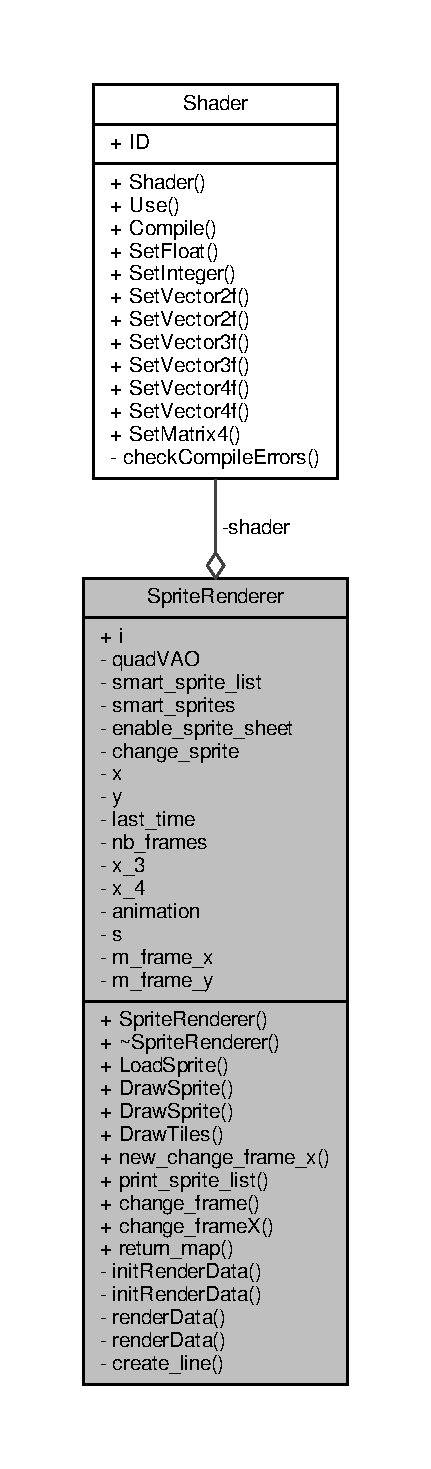
\includegraphics[height=550pt]{classSpriteRenderer__coll__graph}
\end{center}
\end{figure}
\subsection*{Public Member Functions}
\begin{DoxyCompactItemize}
\item 
\hyperlink{classSpriteRenderer_a104f22e721b6d2d1b5e418880dda52a0}{Sprite\+Renderer} (\hyperlink{classShader}{Shader} $\ast$\hyperlink{classSpriteRenderer_a03aa49d90735e23e09f2e0b24da3bd5b}{shader})
\item 
\hyperlink{classSpriteRenderer_ae53730ef86000bf59905c2cf67e4d3a4}{$\sim$\+Sprite\+Renderer} ()
\item 
void \hyperlink{classSpriteRenderer_ab3e76fbe6cbb4ff8be6858cd843dee6c}{Load\+Sprite} (std\+::string, bool i\+\_\+am\+\_\+a\+\_\+sprite\+\_\+sheet, bool \hyperlink{classSpriteRenderer_addcfaa66a79d98c20449119bfc4f4cb2}{change\+\_\+frame}, const unsigned int \&x\+\_\+frame, const unsigned int \&y\+\_\+frame, const float \&incrementer, glm\+::vec2 position, glm\+::vec2 size=glm\+::vec2(10.\+0f, 10.\+0f), float rotate=0.\+0f, glm\+::vec3 color=glm\+::vec3(1.\+0f), glm\+::vec2 m\+\_\+frames=glm\+::vec2(0, 0))
\item 
void \hyperlink{classSpriteRenderer_aea1b4cf018526ae5c98eb66b446a2105}{Draw\+Sprite} (\hyperlink{classTexture2D}{Texture2D} \&texture, bool i\+\_\+am\+\_\+a\+\_\+sprite\+\_\+sheet, bool \hyperlink{classSpriteRenderer_addcfaa66a79d98c20449119bfc4f4cb2}{change\+\_\+frame}, const unsigned int \&x\+\_\+frame, const unsigned int \&y\+\_\+frame, const float \&incrementer, glm\+::vec2 position, glm\+::vec2 size=glm\+::vec2(10.\+0f, 10.\+0f), float rotate=0.\+0f, glm\+::vec3 color=glm\+::vec3(1.\+0f), glm\+::vec2 m\+\_\+frames=glm\+::vec2(0, 0))
\item 
void \hyperlink{classSpriteRenderer_aca1cf0c8ae37192f5d67662215eedf30}{Draw\+Sprite} (\hyperlink{classTexture2D}{Texture2D} \&texture, std\+::string, std\+::unordered\+\_\+map$<$ std\+::string, std\+::shared\+\_\+ptr$<$ \hyperlink{classsprite}{sprite} $>$$>$)
\item 
void \hyperlink{classSpriteRenderer_a0fa081d0a2c4cfdd042b423b12a9c10a}{Draw\+Tiles} (\hyperlink{classTexture2D}{Texture2D} \&texture, std\+::shared\+\_\+ptr$<$ \hyperlink{classsprite}{sprite} $>$ \&\hyperlink{classSpriteRenderer_a51d86fab88b20a802abd8e2333f920a7}{s})
\item 
void \hyperlink{classSpriteRenderer_aec4b432ac6c814cf7ccfe4ca775d7b1f}{new\+\_\+change\+\_\+frame\+\_\+x} (std\+::string key, int frame\+\_\+x, int frame\+\_\+y)
\item 
void \hyperlink{classSpriteRenderer_ae59ff1d27c7df21abb3154b2048d062b}{print\+\_\+sprite\+\_\+list} ()
\item 
void \hyperlink{classSpriteRenderer_addcfaa66a79d98c20449119bfc4f4cb2}{change\+\_\+frame} (int frame)
\item 
void \hyperlink{classSpriteRenderer_af17c77d882bb7140b3cde275fe270304}{change\+\_\+frameX} (int frame)
\item 
std\+::unordered\+\_\+map$<$ std\+::string, std\+::shared\+\_\+ptr$<$ \hyperlink{classsprite}{sprite} $>$ $>$ \hyperlink{classSpriteRenderer_a8c59dae5d92f767afcd55e83f8fb128c}{return\+\_\+map} ()
\end{DoxyCompactItemize}
\subsection*{Public Attributes}
\begin{DoxyCompactItemize}
\item 
float \hyperlink{classSpriteRenderer_acac67b549358ea6335e0310531005382}{i} = 0
\end{DoxyCompactItemize}
\subsection*{Private Member Functions}
\begin{DoxyCompactItemize}
\item 
void \hyperlink{classSpriteRenderer_a45cb93ead211846b0154a8f49b189c50}{init\+Render\+Data} (int \hyperlink{classSpriteRenderer_a448f55e5de2b2b31a641d65e148fb99b}{x})
\item 
void \hyperlink{classSpriteRenderer_ab88c5fde8d172186b73682e871a8bc40}{init\+Render\+Data} (int \hyperlink{classSpriteRenderer_a448f55e5de2b2b31a641d65e148fb99b}{x}, float change\+\_\+frame\+\_\+animation)
\item 
void \hyperlink{classSpriteRenderer_a43f81b7c19394f08227fa5c0f66c9199}{render\+Data} ()
\item 
void \hyperlink{classSpriteRenderer_a4ecc9a7ab7334f2a44cfa2db2f2ca678}{render\+Data} (unsigned int num\+\_\+x\+\_\+frame, unsigned int num\+\_\+y\+\_\+frames, float x\+\_\+frame, float y\+\_\+frame)
\item 
void \hyperlink{classSpriteRenderer_ac18cdf1f92c62b8de313c3e3a7e78621}{create\+\_\+line} (float x\+\_\+start, float y\+\_\+start, float x\+\_\+end, float y\+\_\+end)
\end{DoxyCompactItemize}
\subsection*{Private Attributes}
\begin{DoxyCompactItemize}
\item 
\hyperlink{classShader}{Shader} $\ast$ \hyperlink{classSpriteRenderer_a03aa49d90735e23e09f2e0b24da3bd5b}{shader}
\item 
unsigned int \hyperlink{classSpriteRenderer_a4b15d434e41329a5bea98c6ed1167f21}{quad\+V\+AO}
\item 
std\+::unordered\+\_\+map$<$ std\+::string, std\+::shared\+\_\+ptr$<$ \hyperlink{classsprite}{sprite} $>$ $>$ \hyperlink{classSpriteRenderer_ac167a60d32bf39893efe7f3b15df8af2}{smart\+\_\+sprite\+\_\+list}
\item 
std\+::shared\+\_\+ptr$<$ \hyperlink{classsprite}{sprite} $>$ \hyperlink{classSpriteRenderer_a763db8f0194a6e600c1df98a664abd57}{smart\+\_\+sprites}
\item 
bool \hyperlink{classSpriteRenderer_a882741e00a2220718d79b3ee563e94ed}{enable\+\_\+sprite\+\_\+sheet}
\item 
bool \hyperlink{classSpriteRenderer_a9c38d82e567beef27ba6df93b34a3dc7}{change\+\_\+sprite}
\item 
unsigned int \hyperlink{classSpriteRenderer_a448f55e5de2b2b31a641d65e148fb99b}{x}
\item 
unsigned int \hyperlink{classSpriteRenderer_a5a89882a658f79d41eb498055c9ee2ba}{y}
\item 
double \hyperlink{classSpriteRenderer_a1a4ce8c054473e27f1d978f4f884bd19}{last\+\_\+time} = glfw\+Get\+Time()
\item 
int \hyperlink{classSpriteRenderer_a67d2f35b38997c78eb63a92fbc6bcdee}{nb\+\_\+frames} = 0
\item 
bool \hyperlink{classSpriteRenderer_a79a58b0a7a37be0f6a3d014e4529917f}{x\+\_\+3} = false
\item 
bool \hyperlink{classSpriteRenderer_a1f1b9ed16ab7b22808b2ba3e056762cd}{x\+\_\+4} = false
\item 
float \hyperlink{classSpriteRenderer_ab4358a0e1fbfb0e127e54c5289503628}{animation} = 0
\item 
float \hyperlink{classSpriteRenderer_a51d86fab88b20a802abd8e2333f920a7}{s} = 0.\+0f
\item 
int \hyperlink{classSpriteRenderer_ac99efebafb5bac3faac1620d250e0bc0}{m\+\_\+frame\+\_\+x}
\item 
int \hyperlink{classSpriteRenderer_a85e43c28ae6e6934bdbf6719e3c2ce20}{m\+\_\+frame\+\_\+y}
\end{DoxyCompactItemize}


\subsection{Constructor \& Destructor Documentation}
\mbox{\Hypertarget{classSpriteRenderer_a104f22e721b6d2d1b5e418880dda52a0}\label{classSpriteRenderer_a104f22e721b6d2d1b5e418880dda52a0}} 
\index{Sprite\+Renderer@{Sprite\+Renderer}!Sprite\+Renderer@{Sprite\+Renderer}}
\index{Sprite\+Renderer@{Sprite\+Renderer}!Sprite\+Renderer@{Sprite\+Renderer}}
\subsubsection{\texorpdfstring{Sprite\+Renderer()}{SpriteRenderer()}}
{\footnotesize\ttfamily Sprite\+Renderer\+::\+Sprite\+Renderer (\begin{DoxyParamCaption}\item[{\hyperlink{classShader}{Shader} $\ast$}]{shader }\end{DoxyParamCaption})}

\mbox{\Hypertarget{classSpriteRenderer_ae53730ef86000bf59905c2cf67e4d3a4}\label{classSpriteRenderer_ae53730ef86000bf59905c2cf67e4d3a4}} 
\index{Sprite\+Renderer@{Sprite\+Renderer}!````~Sprite\+Renderer@{$\sim$\+Sprite\+Renderer}}
\index{````~Sprite\+Renderer@{$\sim$\+Sprite\+Renderer}!Sprite\+Renderer@{Sprite\+Renderer}}
\subsubsection{\texorpdfstring{$\sim$\+Sprite\+Renderer()}{~SpriteRenderer()}}
{\footnotesize\ttfamily Sprite\+Renderer\+::$\sim$\+Sprite\+Renderer (\begin{DoxyParamCaption}{ }\end{DoxyParamCaption})}



\subsection{Member Function Documentation}
\mbox{\Hypertarget{classSpriteRenderer_addcfaa66a79d98c20449119bfc4f4cb2}\label{classSpriteRenderer_addcfaa66a79d98c20449119bfc4f4cb2}} 
\index{Sprite\+Renderer@{Sprite\+Renderer}!change\+\_\+frame@{change\+\_\+frame}}
\index{change\+\_\+frame@{change\+\_\+frame}!Sprite\+Renderer@{Sprite\+Renderer}}
\subsubsection{\texorpdfstring{change\+\_\+frame()}{change\_frame()}}
{\footnotesize\ttfamily void Sprite\+Renderer\+::change\+\_\+frame (\begin{DoxyParamCaption}\item[{int}]{frame }\end{DoxyParamCaption})\hspace{0.3cm}{\ttfamily [inline]}}

\mbox{\Hypertarget{classSpriteRenderer_af17c77d882bb7140b3cde275fe270304}\label{classSpriteRenderer_af17c77d882bb7140b3cde275fe270304}} 
\index{Sprite\+Renderer@{Sprite\+Renderer}!change\+\_\+frameX@{change\+\_\+frameX}}
\index{change\+\_\+frameX@{change\+\_\+frameX}!Sprite\+Renderer@{Sprite\+Renderer}}
\subsubsection{\texorpdfstring{change\+\_\+frame\+X()}{change\_frameX()}}
{\footnotesize\ttfamily void Sprite\+Renderer\+::change\+\_\+frameX (\begin{DoxyParamCaption}\item[{int}]{frame }\end{DoxyParamCaption})\hspace{0.3cm}{\ttfamily [inline]}}

\mbox{\Hypertarget{classSpriteRenderer_ac18cdf1f92c62b8de313c3e3a7e78621}\label{classSpriteRenderer_ac18cdf1f92c62b8de313c3e3a7e78621}} 
\index{Sprite\+Renderer@{Sprite\+Renderer}!create\+\_\+line@{create\+\_\+line}}
\index{create\+\_\+line@{create\+\_\+line}!Sprite\+Renderer@{Sprite\+Renderer}}
\subsubsection{\texorpdfstring{create\+\_\+line()}{create\_line()}}
{\footnotesize\ttfamily void Sprite\+Renderer\+::create\+\_\+line (\begin{DoxyParamCaption}\item[{float}]{x\+\_\+start,  }\item[{float}]{y\+\_\+start,  }\item[{float}]{x\+\_\+end,  }\item[{float}]{y\+\_\+end }\end{DoxyParamCaption})\hspace{0.3cm}{\ttfamily [private]}}

\mbox{\Hypertarget{classSpriteRenderer_aea1b4cf018526ae5c98eb66b446a2105}\label{classSpriteRenderer_aea1b4cf018526ae5c98eb66b446a2105}} 
\index{Sprite\+Renderer@{Sprite\+Renderer}!Draw\+Sprite@{Draw\+Sprite}}
\index{Draw\+Sprite@{Draw\+Sprite}!Sprite\+Renderer@{Sprite\+Renderer}}
\subsubsection{\texorpdfstring{Draw\+Sprite()}{DrawSprite()}\hspace{0.1cm}{\footnotesize\ttfamily [1/2]}}
{\footnotesize\ttfamily void Sprite\+Renderer\+::\+Draw\+Sprite (\begin{DoxyParamCaption}\item[{\hyperlink{classTexture2D}{Texture2D} \&}]{texture,  }\item[{bool}]{i\+\_\+am\+\_\+a\+\_\+sprite\+\_\+sheet,  }\item[{bool}]{change\+\_\+frame,  }\item[{const unsigned int \&}]{x\+\_\+frame,  }\item[{const unsigned int \&}]{y\+\_\+frame,  }\item[{const float \&}]{incrementer,  }\item[{glm\+::vec2}]{position,  }\item[{glm\+::vec2}]{size = {\ttfamily glm\+:\+:vec2(10.0f,~10.0f)},  }\item[{float}]{rotate = {\ttfamily 0.0f},  }\item[{glm\+::vec3}]{color = {\ttfamily glm\+:\+:vec3(1.0f)},  }\item[{glm\+::vec2}]{m\+\_\+frames = {\ttfamily glm\+:\+:vec2(0,~0)} }\end{DoxyParamCaption})}

\mbox{\Hypertarget{classSpriteRenderer_aca1cf0c8ae37192f5d67662215eedf30}\label{classSpriteRenderer_aca1cf0c8ae37192f5d67662215eedf30}} 
\index{Sprite\+Renderer@{Sprite\+Renderer}!Draw\+Sprite@{Draw\+Sprite}}
\index{Draw\+Sprite@{Draw\+Sprite}!Sprite\+Renderer@{Sprite\+Renderer}}
\subsubsection{\texorpdfstring{Draw\+Sprite()}{DrawSprite()}\hspace{0.1cm}{\footnotesize\ttfamily [2/2]}}
{\footnotesize\ttfamily void Sprite\+Renderer\+::\+Draw\+Sprite (\begin{DoxyParamCaption}\item[{\hyperlink{classTexture2D}{Texture2D} \&}]{texture,  }\item[{std\+::string}]{key,  }\item[{std\+::unordered\+\_\+map$<$ std\+::string, std\+::shared\+\_\+ptr$<$ \hyperlink{classsprite}{sprite} $>$$>$}]{sprite\+\_\+map }\end{DoxyParamCaption})}

\mbox{\Hypertarget{classSpriteRenderer_a0fa081d0a2c4cfdd042b423b12a9c10a}\label{classSpriteRenderer_a0fa081d0a2c4cfdd042b423b12a9c10a}} 
\index{Sprite\+Renderer@{Sprite\+Renderer}!Draw\+Tiles@{Draw\+Tiles}}
\index{Draw\+Tiles@{Draw\+Tiles}!Sprite\+Renderer@{Sprite\+Renderer}}
\subsubsection{\texorpdfstring{Draw\+Tiles()}{DrawTiles()}}
{\footnotesize\ttfamily void Sprite\+Renderer\+::\+Draw\+Tiles (\begin{DoxyParamCaption}\item[{\hyperlink{classTexture2D}{Texture2D} \&}]{texture,  }\item[{std\+::shared\+\_\+ptr$<$ \hyperlink{classsprite}{sprite} $>$ \&}]{s }\end{DoxyParamCaption})}

\mbox{\Hypertarget{classSpriteRenderer_a45cb93ead211846b0154a8f49b189c50}\label{classSpriteRenderer_a45cb93ead211846b0154a8f49b189c50}} 
\index{Sprite\+Renderer@{Sprite\+Renderer}!init\+Render\+Data@{init\+Render\+Data}}
\index{init\+Render\+Data@{init\+Render\+Data}!Sprite\+Renderer@{Sprite\+Renderer}}
\subsubsection{\texorpdfstring{init\+Render\+Data()}{initRenderData()}\hspace{0.1cm}{\footnotesize\ttfamily [1/2]}}
{\footnotesize\ttfamily void Sprite\+Renderer\+::init\+Render\+Data (\begin{DoxyParamCaption}\item[{int}]{x }\end{DoxyParamCaption})\hspace{0.3cm}{\ttfamily [private]}}

\mbox{\Hypertarget{classSpriteRenderer_ab88c5fde8d172186b73682e871a8bc40}\label{classSpriteRenderer_ab88c5fde8d172186b73682e871a8bc40}} 
\index{Sprite\+Renderer@{Sprite\+Renderer}!init\+Render\+Data@{init\+Render\+Data}}
\index{init\+Render\+Data@{init\+Render\+Data}!Sprite\+Renderer@{Sprite\+Renderer}}
\subsubsection{\texorpdfstring{init\+Render\+Data()}{initRenderData()}\hspace{0.1cm}{\footnotesize\ttfamily [2/2]}}
{\footnotesize\ttfamily void Sprite\+Renderer\+::init\+Render\+Data (\begin{DoxyParamCaption}\item[{int}]{x,  }\item[{float}]{change\+\_\+frame\+\_\+animation }\end{DoxyParamCaption})\hspace{0.3cm}{\ttfamily [private]}}

\mbox{\Hypertarget{classSpriteRenderer_ab3e76fbe6cbb4ff8be6858cd843dee6c}\label{classSpriteRenderer_ab3e76fbe6cbb4ff8be6858cd843dee6c}} 
\index{Sprite\+Renderer@{Sprite\+Renderer}!Load\+Sprite@{Load\+Sprite}}
\index{Load\+Sprite@{Load\+Sprite}!Sprite\+Renderer@{Sprite\+Renderer}}
\subsubsection{\texorpdfstring{Load\+Sprite()}{LoadSprite()}}
{\footnotesize\ttfamily void Sprite\+Renderer\+::\+Load\+Sprite (\begin{DoxyParamCaption}\item[{std\+::string}]{key,  }\item[{bool}]{i\+\_\+am\+\_\+a\+\_\+sprite\+\_\+sheet,  }\item[{bool}]{change\+\_\+frame,  }\item[{const unsigned int \&}]{x\+\_\+frame,  }\item[{const unsigned int \&}]{y\+\_\+frame,  }\item[{const float \&}]{incrementer,  }\item[{glm\+::vec2}]{position,  }\item[{glm\+::vec2}]{size = {\ttfamily glm\+:\+:vec2(10.0f,~10.0f)},  }\item[{float}]{rotate = {\ttfamily 0.0f},  }\item[{glm\+::vec3}]{color = {\ttfamily glm\+:\+:vec3(1.0f)},  }\item[{glm\+::vec2}]{m\+\_\+frames = {\ttfamily glm\+:\+:vec2(0,~0)} }\end{DoxyParamCaption})}

\mbox{\Hypertarget{classSpriteRenderer_aec4b432ac6c814cf7ccfe4ca775d7b1f}\label{classSpriteRenderer_aec4b432ac6c814cf7ccfe4ca775d7b1f}} 
\index{Sprite\+Renderer@{Sprite\+Renderer}!new\+\_\+change\+\_\+frame\+\_\+x@{new\+\_\+change\+\_\+frame\+\_\+x}}
\index{new\+\_\+change\+\_\+frame\+\_\+x@{new\+\_\+change\+\_\+frame\+\_\+x}!Sprite\+Renderer@{Sprite\+Renderer}}
\subsubsection{\texorpdfstring{new\+\_\+change\+\_\+frame\+\_\+x()}{new\_change\_frame\_x()}}
{\footnotesize\ttfamily void Sprite\+Renderer\+::new\+\_\+change\+\_\+frame\+\_\+x (\begin{DoxyParamCaption}\item[{std\+::string}]{key,  }\item[{int}]{frame\+\_\+x,  }\item[{int}]{frame\+\_\+y }\end{DoxyParamCaption})\hspace{0.3cm}{\ttfamily [inline]}}

\mbox{\Hypertarget{classSpriteRenderer_ae59ff1d27c7df21abb3154b2048d062b}\label{classSpriteRenderer_ae59ff1d27c7df21abb3154b2048d062b}} 
\index{Sprite\+Renderer@{Sprite\+Renderer}!print\+\_\+sprite\+\_\+list@{print\+\_\+sprite\+\_\+list}}
\index{print\+\_\+sprite\+\_\+list@{print\+\_\+sprite\+\_\+list}!Sprite\+Renderer@{Sprite\+Renderer}}
\subsubsection{\texorpdfstring{print\+\_\+sprite\+\_\+list()}{print\_sprite\_list()}}
{\footnotesize\ttfamily void Sprite\+Renderer\+::print\+\_\+sprite\+\_\+list (\begin{DoxyParamCaption}{ }\end{DoxyParamCaption})\hspace{0.3cm}{\ttfamily [inline]}}

\mbox{\Hypertarget{classSpriteRenderer_a43f81b7c19394f08227fa5c0f66c9199}\label{classSpriteRenderer_a43f81b7c19394f08227fa5c0f66c9199}} 
\index{Sprite\+Renderer@{Sprite\+Renderer}!render\+Data@{render\+Data}}
\index{render\+Data@{render\+Data}!Sprite\+Renderer@{Sprite\+Renderer}}
\subsubsection{\texorpdfstring{render\+Data()}{renderData()}\hspace{0.1cm}{\footnotesize\ttfamily [1/2]}}
{\footnotesize\ttfamily void Sprite\+Renderer\+::render\+Data (\begin{DoxyParamCaption}{ }\end{DoxyParamCaption})\hspace{0.3cm}{\ttfamily [private]}}

\mbox{\Hypertarget{classSpriteRenderer_a4ecc9a7ab7334f2a44cfa2db2f2ca678}\label{classSpriteRenderer_a4ecc9a7ab7334f2a44cfa2db2f2ca678}} 
\index{Sprite\+Renderer@{Sprite\+Renderer}!render\+Data@{render\+Data}}
\index{render\+Data@{render\+Data}!Sprite\+Renderer@{Sprite\+Renderer}}
\subsubsection{\texorpdfstring{render\+Data()}{renderData()}\hspace{0.1cm}{\footnotesize\ttfamily [2/2]}}
{\footnotesize\ttfamily void Sprite\+Renderer\+::render\+Data (\begin{DoxyParamCaption}\item[{unsigned int}]{num\+\_\+x\+\_\+frame,  }\item[{unsigned int}]{num\+\_\+y\+\_\+frames,  }\item[{float}]{x\+\_\+frame,  }\item[{float}]{y\+\_\+frame }\end{DoxyParamCaption})\hspace{0.3cm}{\ttfamily [private]}}

\mbox{\Hypertarget{classSpriteRenderer_a8c59dae5d92f767afcd55e83f8fb128c}\label{classSpriteRenderer_a8c59dae5d92f767afcd55e83f8fb128c}} 
\index{Sprite\+Renderer@{Sprite\+Renderer}!return\+\_\+map@{return\+\_\+map}}
\index{return\+\_\+map@{return\+\_\+map}!Sprite\+Renderer@{Sprite\+Renderer}}
\subsubsection{\texorpdfstring{return\+\_\+map()}{return\_map()}}
{\footnotesize\ttfamily std\+::unordered\+\_\+map$<$std\+::string, std\+::shared\+\_\+ptr$<$\hyperlink{classsprite}{sprite}$>$ $>$ Sprite\+Renderer\+::return\+\_\+map (\begin{DoxyParamCaption}{ }\end{DoxyParamCaption})\hspace{0.3cm}{\ttfamily [inline]}}



\subsection{Member Data Documentation}
\mbox{\Hypertarget{classSpriteRenderer_ab4358a0e1fbfb0e127e54c5289503628}\label{classSpriteRenderer_ab4358a0e1fbfb0e127e54c5289503628}} 
\index{Sprite\+Renderer@{Sprite\+Renderer}!animation@{animation}}
\index{animation@{animation}!Sprite\+Renderer@{Sprite\+Renderer}}
\subsubsection{\texorpdfstring{animation}{animation}}
{\footnotesize\ttfamily float Sprite\+Renderer\+::animation = 0\hspace{0.3cm}{\ttfamily [private]}}

\mbox{\Hypertarget{classSpriteRenderer_a9c38d82e567beef27ba6df93b34a3dc7}\label{classSpriteRenderer_a9c38d82e567beef27ba6df93b34a3dc7}} 
\index{Sprite\+Renderer@{Sprite\+Renderer}!change\+\_\+sprite@{change\+\_\+sprite}}
\index{change\+\_\+sprite@{change\+\_\+sprite}!Sprite\+Renderer@{Sprite\+Renderer}}
\subsubsection{\texorpdfstring{change\+\_\+sprite}{change\_sprite}}
{\footnotesize\ttfamily bool Sprite\+Renderer\+::change\+\_\+sprite\hspace{0.3cm}{\ttfamily [private]}}

\mbox{\Hypertarget{classSpriteRenderer_a882741e00a2220718d79b3ee563e94ed}\label{classSpriteRenderer_a882741e00a2220718d79b3ee563e94ed}} 
\index{Sprite\+Renderer@{Sprite\+Renderer}!enable\+\_\+sprite\+\_\+sheet@{enable\+\_\+sprite\+\_\+sheet}}
\index{enable\+\_\+sprite\+\_\+sheet@{enable\+\_\+sprite\+\_\+sheet}!Sprite\+Renderer@{Sprite\+Renderer}}
\subsubsection{\texorpdfstring{enable\+\_\+sprite\+\_\+sheet}{enable\_sprite\_sheet}}
{\footnotesize\ttfamily bool Sprite\+Renderer\+::enable\+\_\+sprite\+\_\+sheet\hspace{0.3cm}{\ttfamily [private]}}

\mbox{\Hypertarget{classSpriteRenderer_acac67b549358ea6335e0310531005382}\label{classSpriteRenderer_acac67b549358ea6335e0310531005382}} 
\index{Sprite\+Renderer@{Sprite\+Renderer}!i@{i}}
\index{i@{i}!Sprite\+Renderer@{Sprite\+Renderer}}
\subsubsection{\texorpdfstring{i}{i}}
{\footnotesize\ttfamily float Sprite\+Renderer\+::i = 0}

\mbox{\Hypertarget{classSpriteRenderer_a1a4ce8c054473e27f1d978f4f884bd19}\label{classSpriteRenderer_a1a4ce8c054473e27f1d978f4f884bd19}} 
\index{Sprite\+Renderer@{Sprite\+Renderer}!last\+\_\+time@{last\+\_\+time}}
\index{last\+\_\+time@{last\+\_\+time}!Sprite\+Renderer@{Sprite\+Renderer}}
\subsubsection{\texorpdfstring{last\+\_\+time}{last\_time}}
{\footnotesize\ttfamily double Sprite\+Renderer\+::last\+\_\+time = glfw\+Get\+Time()\hspace{0.3cm}{\ttfamily [private]}}

\mbox{\Hypertarget{classSpriteRenderer_ac99efebafb5bac3faac1620d250e0bc0}\label{classSpriteRenderer_ac99efebafb5bac3faac1620d250e0bc0}} 
\index{Sprite\+Renderer@{Sprite\+Renderer}!m\+\_\+frame\+\_\+x@{m\+\_\+frame\+\_\+x}}
\index{m\+\_\+frame\+\_\+x@{m\+\_\+frame\+\_\+x}!Sprite\+Renderer@{Sprite\+Renderer}}
\subsubsection{\texorpdfstring{m\+\_\+frame\+\_\+x}{m\_frame\_x}}
{\footnotesize\ttfamily int Sprite\+Renderer\+::m\+\_\+frame\+\_\+x\hspace{0.3cm}{\ttfamily [private]}}

\mbox{\Hypertarget{classSpriteRenderer_a85e43c28ae6e6934bdbf6719e3c2ce20}\label{classSpriteRenderer_a85e43c28ae6e6934bdbf6719e3c2ce20}} 
\index{Sprite\+Renderer@{Sprite\+Renderer}!m\+\_\+frame\+\_\+y@{m\+\_\+frame\+\_\+y}}
\index{m\+\_\+frame\+\_\+y@{m\+\_\+frame\+\_\+y}!Sprite\+Renderer@{Sprite\+Renderer}}
\subsubsection{\texorpdfstring{m\+\_\+frame\+\_\+y}{m\_frame\_y}}
{\footnotesize\ttfamily int Sprite\+Renderer\+::m\+\_\+frame\+\_\+y\hspace{0.3cm}{\ttfamily [private]}}

\mbox{\Hypertarget{classSpriteRenderer_a67d2f35b38997c78eb63a92fbc6bcdee}\label{classSpriteRenderer_a67d2f35b38997c78eb63a92fbc6bcdee}} 
\index{Sprite\+Renderer@{Sprite\+Renderer}!nb\+\_\+frames@{nb\+\_\+frames}}
\index{nb\+\_\+frames@{nb\+\_\+frames}!Sprite\+Renderer@{Sprite\+Renderer}}
\subsubsection{\texorpdfstring{nb\+\_\+frames}{nb\_frames}}
{\footnotesize\ttfamily int Sprite\+Renderer\+::nb\+\_\+frames = 0\hspace{0.3cm}{\ttfamily [private]}}

\mbox{\Hypertarget{classSpriteRenderer_a4b15d434e41329a5bea98c6ed1167f21}\label{classSpriteRenderer_a4b15d434e41329a5bea98c6ed1167f21}} 
\index{Sprite\+Renderer@{Sprite\+Renderer}!quad\+V\+AO@{quad\+V\+AO}}
\index{quad\+V\+AO@{quad\+V\+AO}!Sprite\+Renderer@{Sprite\+Renderer}}
\subsubsection{\texorpdfstring{quad\+V\+AO}{quadVAO}}
{\footnotesize\ttfamily unsigned int Sprite\+Renderer\+::quad\+V\+AO\hspace{0.3cm}{\ttfamily [private]}}

\mbox{\Hypertarget{classSpriteRenderer_a51d86fab88b20a802abd8e2333f920a7}\label{classSpriteRenderer_a51d86fab88b20a802abd8e2333f920a7}} 
\index{Sprite\+Renderer@{Sprite\+Renderer}!s@{s}}
\index{s@{s}!Sprite\+Renderer@{Sprite\+Renderer}}
\subsubsection{\texorpdfstring{s}{s}}
{\footnotesize\ttfamily float Sprite\+Renderer\+::s = 0.\+0f\hspace{0.3cm}{\ttfamily [private]}}

\mbox{\Hypertarget{classSpriteRenderer_a03aa49d90735e23e09f2e0b24da3bd5b}\label{classSpriteRenderer_a03aa49d90735e23e09f2e0b24da3bd5b}} 
\index{Sprite\+Renderer@{Sprite\+Renderer}!shader@{shader}}
\index{shader@{shader}!Sprite\+Renderer@{Sprite\+Renderer}}
\subsubsection{\texorpdfstring{shader}{shader}}
{\footnotesize\ttfamily \hyperlink{classShader}{Shader}$\ast$ Sprite\+Renderer\+::shader\hspace{0.3cm}{\ttfamily [private]}}

\mbox{\Hypertarget{classSpriteRenderer_ac167a60d32bf39893efe7f3b15df8af2}\label{classSpriteRenderer_ac167a60d32bf39893efe7f3b15df8af2}} 
\index{Sprite\+Renderer@{Sprite\+Renderer}!smart\+\_\+sprite\+\_\+list@{smart\+\_\+sprite\+\_\+list}}
\index{smart\+\_\+sprite\+\_\+list@{smart\+\_\+sprite\+\_\+list}!Sprite\+Renderer@{Sprite\+Renderer}}
\subsubsection{\texorpdfstring{smart\+\_\+sprite\+\_\+list}{smart\_sprite\_list}}
{\footnotesize\ttfamily std\+::unordered\+\_\+map$<$std\+::string, std\+::shared\+\_\+ptr$<$\hyperlink{classsprite}{sprite}$>$ $>$ Sprite\+Renderer\+::smart\+\_\+sprite\+\_\+list\hspace{0.3cm}{\ttfamily [private]}}

\mbox{\Hypertarget{classSpriteRenderer_a763db8f0194a6e600c1df98a664abd57}\label{classSpriteRenderer_a763db8f0194a6e600c1df98a664abd57}} 
\index{Sprite\+Renderer@{Sprite\+Renderer}!smart\+\_\+sprites@{smart\+\_\+sprites}}
\index{smart\+\_\+sprites@{smart\+\_\+sprites}!Sprite\+Renderer@{Sprite\+Renderer}}
\subsubsection{\texorpdfstring{smart\+\_\+sprites}{smart\_sprites}}
{\footnotesize\ttfamily std\+::shared\+\_\+ptr$<$\hyperlink{classsprite}{sprite}$>$ Sprite\+Renderer\+::smart\+\_\+sprites\hspace{0.3cm}{\ttfamily [private]}}

\mbox{\Hypertarget{classSpriteRenderer_a448f55e5de2b2b31a641d65e148fb99b}\label{classSpriteRenderer_a448f55e5de2b2b31a641d65e148fb99b}} 
\index{Sprite\+Renderer@{Sprite\+Renderer}!x@{x}}
\index{x@{x}!Sprite\+Renderer@{Sprite\+Renderer}}
\subsubsection{\texorpdfstring{x}{x}}
{\footnotesize\ttfamily unsigned int Sprite\+Renderer\+::x\hspace{0.3cm}{\ttfamily [private]}}

\mbox{\Hypertarget{classSpriteRenderer_a79a58b0a7a37be0f6a3d014e4529917f}\label{classSpriteRenderer_a79a58b0a7a37be0f6a3d014e4529917f}} 
\index{Sprite\+Renderer@{Sprite\+Renderer}!x\+\_\+3@{x\+\_\+3}}
\index{x\+\_\+3@{x\+\_\+3}!Sprite\+Renderer@{Sprite\+Renderer}}
\subsubsection{\texorpdfstring{x\+\_\+3}{x\_3}}
{\footnotesize\ttfamily bool Sprite\+Renderer\+::x\+\_\+3 = false\hspace{0.3cm}{\ttfamily [private]}}

\mbox{\Hypertarget{classSpriteRenderer_a1f1b9ed16ab7b22808b2ba3e056762cd}\label{classSpriteRenderer_a1f1b9ed16ab7b22808b2ba3e056762cd}} 
\index{Sprite\+Renderer@{Sprite\+Renderer}!x\+\_\+4@{x\+\_\+4}}
\index{x\+\_\+4@{x\+\_\+4}!Sprite\+Renderer@{Sprite\+Renderer}}
\subsubsection{\texorpdfstring{x\+\_\+4}{x\_4}}
{\footnotesize\ttfamily bool Sprite\+Renderer\+::x\+\_\+4 = false\hspace{0.3cm}{\ttfamily [private]}}

\mbox{\Hypertarget{classSpriteRenderer_a5a89882a658f79d41eb498055c9ee2ba}\label{classSpriteRenderer_a5a89882a658f79d41eb498055c9ee2ba}} 
\index{Sprite\+Renderer@{Sprite\+Renderer}!y@{y}}
\index{y@{y}!Sprite\+Renderer@{Sprite\+Renderer}}
\subsubsection{\texorpdfstring{y}{y}}
{\footnotesize\ttfamily unsigned int Sprite\+Renderer\+::y\hspace{0.3cm}{\ttfamily [private]}}



The documentation for this class was generated from the following files\+:\begin{DoxyCompactItemize}
\item 
/mnt/hdd/\+C0de/smart\+\_\+engine/include/\hyperlink{sprite__renderer_8h}{sprite\+\_\+renderer.\+h}\item 
/mnt/hdd/\+C0de/smart\+\_\+engine/src/\hyperlink{sprite__renderer_8cpp}{sprite\+\_\+renderer.\+cpp}\end{DoxyCompactItemize}

\hypertarget{classState}{}\section{State Class Reference}
\label{classState}\index{State@{State}}


{\ttfamily \#include $<$state.\+h$>$}



Inheritance diagram for State\+:
\nopagebreak
\begin{figure}[H]
\begin{center}
\leavevmode
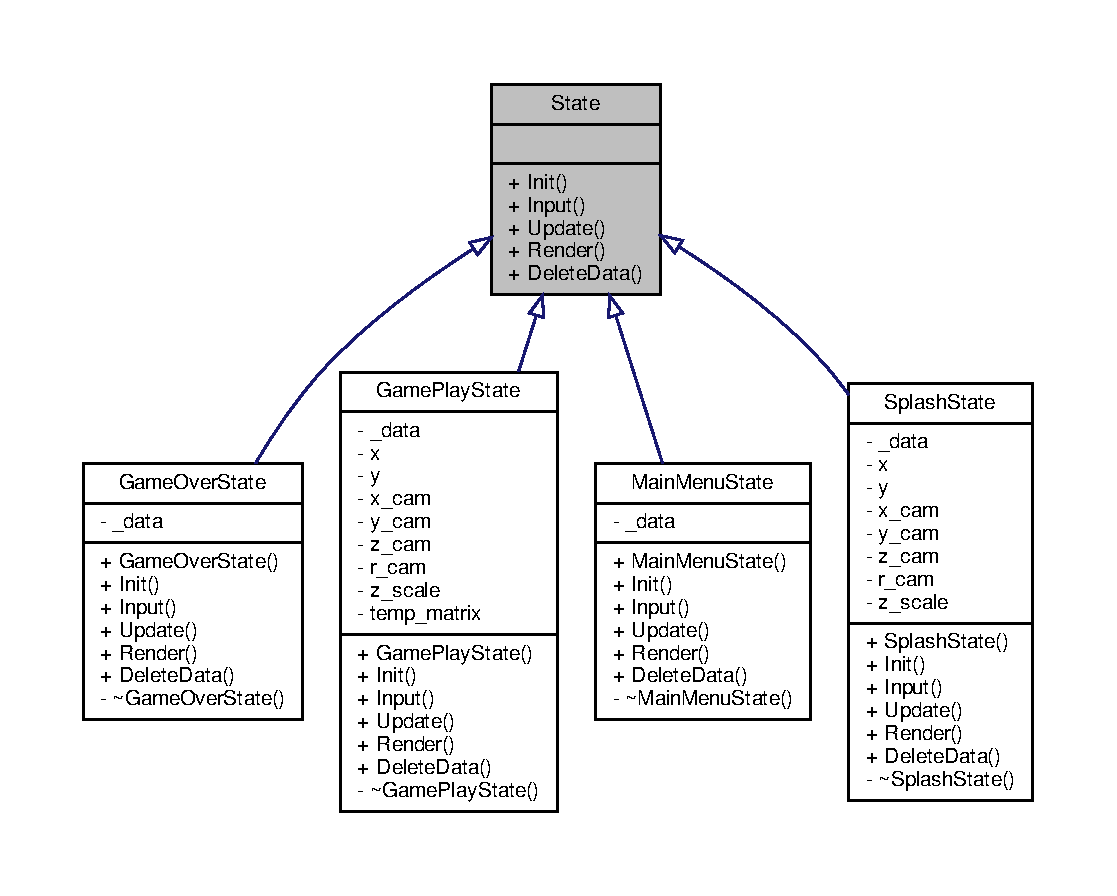
\includegraphics[width=350pt]{classState__inherit__graph}
\end{center}
\end{figure}


Collaboration diagram for State\+:
\nopagebreak
\begin{figure}[H]
\begin{center}
\leavevmode
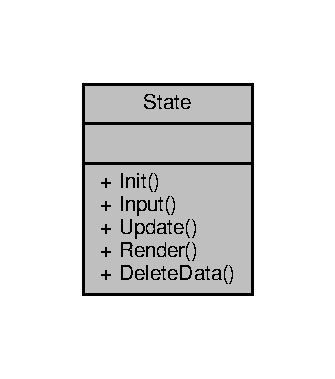
\includegraphics[width=161pt]{classState__coll__graph}
\end{center}
\end{figure}
\subsection*{Public Member Functions}
\begin{DoxyCompactItemize}
\item 
virtual void \hyperlink{classState_a7ab4d8c6aa239a17ed579d89a209b156}{Init} ()=0
\item 
virtual void \hyperlink{classState_a1705412877f37a5cc8fc712542756076}{Input} (float delta)=0
\item 
virtual void \hyperlink{classState_aac0d3fdee1341e168af730b8f31a7bf1}{Update} (float delta)=0
\item 
virtual void \hyperlink{classState_a0e48dfae1e3090630475812681417c5f}{Render} (float delta)=0
\item 
virtual void \hyperlink{classState_ade502eaa386d570e526eb356ffd73fd8}{Delete\+Data} ()=0
\end{DoxyCompactItemize}


\subsection{Member Function Documentation}
\mbox{\Hypertarget{classState_ade502eaa386d570e526eb356ffd73fd8}\label{classState_ade502eaa386d570e526eb356ffd73fd8}} 
\index{State@{State}!Delete\+Data@{Delete\+Data}}
\index{Delete\+Data@{Delete\+Data}!State@{State}}
\subsubsection{\texorpdfstring{Delete\+Data()}{DeleteData()}}
{\footnotesize\ttfamily virtual void State\+::\+Delete\+Data (\begin{DoxyParamCaption}{ }\end{DoxyParamCaption})\hspace{0.3cm}{\ttfamily [pure virtual]}}



Implemented in \hyperlink{classSplashState_aca842c8e3ea2642980569ed3b4bb362a}{Splash\+State}, \hyperlink{classMainMenuState_a52c4dad229a1e9851e8742b81bc30abb}{Main\+Menu\+State}, \hyperlink{classGameOverState_afb6fa68ff0c5e4f83725de8059c4f7c8}{Game\+Over\+State}, and \hyperlink{classGamePlayState_a8a393249f2deabe0fe8f236b4e58cb17}{Game\+Play\+State}.

\mbox{\Hypertarget{classState_a7ab4d8c6aa239a17ed579d89a209b156}\label{classState_a7ab4d8c6aa239a17ed579d89a209b156}} 
\index{State@{State}!Init@{Init}}
\index{Init@{Init}!State@{State}}
\subsubsection{\texorpdfstring{Init()}{Init()}}
{\footnotesize\ttfamily virtual void State\+::\+Init (\begin{DoxyParamCaption}{ }\end{DoxyParamCaption})\hspace{0.3cm}{\ttfamily [pure virtual]}}



Implemented in \hyperlink{classSplashState_ae3e0604da087032c179593c237580988}{Splash\+State}, \hyperlink{classMainMenuState_afab2a9b829a8ef752fed701d5cd260f8}{Main\+Menu\+State}, \hyperlink{classGameOverState_aa3d4f165ff735552f16132e929d369c2}{Game\+Over\+State}, and \hyperlink{classGamePlayState_ae13389eea1f83f27d18ba200f107937d}{Game\+Play\+State}.

\mbox{\Hypertarget{classState_a1705412877f37a5cc8fc712542756076}\label{classState_a1705412877f37a5cc8fc712542756076}} 
\index{State@{State}!Input@{Input}}
\index{Input@{Input}!State@{State}}
\subsubsection{\texorpdfstring{Input()}{Input()}}
{\footnotesize\ttfamily virtual void State\+::\+Input (\begin{DoxyParamCaption}\item[{float}]{delta }\end{DoxyParamCaption})\hspace{0.3cm}{\ttfamily [pure virtual]}}



Implemented in \hyperlink{classSplashState_adb2eb87bd89e41af0c3a9d0903e89450}{Splash\+State}, \hyperlink{classMainMenuState_aa62c91d35b5b4a24c0a13c22020845e8}{Main\+Menu\+State}, \hyperlink{classGameOverState_adb4be2a5c6292d020999c2da9588ebfc}{Game\+Over\+State}, and \hyperlink{classGamePlayState_a3bc9231fd11546b5dd13581ed2aa1afa}{Game\+Play\+State}.

\mbox{\Hypertarget{classState_a0e48dfae1e3090630475812681417c5f}\label{classState_a0e48dfae1e3090630475812681417c5f}} 
\index{State@{State}!Render@{Render}}
\index{Render@{Render}!State@{State}}
\subsubsection{\texorpdfstring{Render()}{Render()}}
{\footnotesize\ttfamily virtual void State\+::\+Render (\begin{DoxyParamCaption}\item[{float}]{delta }\end{DoxyParamCaption})\hspace{0.3cm}{\ttfamily [pure virtual]}}



Implemented in \hyperlink{classSplashState_a5efb6f0ede61ec76ee2dd72a6b24c57c}{Splash\+State}, \hyperlink{classMainMenuState_af675ec319923f1cf22446808a7735dea}{Main\+Menu\+State}, \hyperlink{classGameOverState_ac9c9ef71b0a12940ac5caa7763f23fdc}{Game\+Over\+State}, and \hyperlink{classGamePlayState_a4bd296aa04088a3d8249f569e86f21a7}{Game\+Play\+State}.

\mbox{\Hypertarget{classState_aac0d3fdee1341e168af730b8f31a7bf1}\label{classState_aac0d3fdee1341e168af730b8f31a7bf1}} 
\index{State@{State}!Update@{Update}}
\index{Update@{Update}!State@{State}}
\subsubsection{\texorpdfstring{Update()}{Update()}}
{\footnotesize\ttfamily virtual void State\+::\+Update (\begin{DoxyParamCaption}\item[{float}]{delta }\end{DoxyParamCaption})\hspace{0.3cm}{\ttfamily [pure virtual]}}



Implemented in \hyperlink{classSplashState_af19b293ae1e914e13db4382115e56d2c}{Splash\+State}, \hyperlink{classMainMenuState_a1605be0d2e5228643d911c7069db3196}{Main\+Menu\+State}, \hyperlink{classGameOverState_a4dc49d576a9435531f502660119800a9}{Game\+Over\+State}, and \hyperlink{classGamePlayState_a19bcc1ff2a83a3aa001010ae35d67b85}{Game\+Play\+State}.



The documentation for this class was generated from the following file\+:\begin{DoxyCompactItemize}
\item 
/mnt/hdd/\+C0de/smart\+\_\+engine/include/\hyperlink{state_8h}{state.\+h}\end{DoxyCompactItemize}

\hypertarget{classStateMachine}{}\section{State\+Machine Class Reference}
\label{classStateMachine}\index{State\+Machine@{State\+Machine}}


{\ttfamily \#include $<$state\+\_\+machine.\+h$>$}



Collaboration diagram for State\+Machine\+:
\nopagebreak
\begin{figure}[H]
\begin{center}
\leavevmode
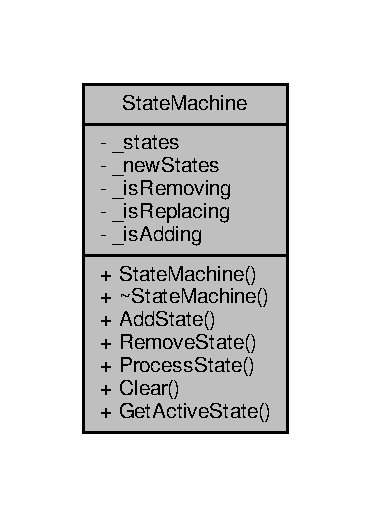
\includegraphics[width=178pt]{classStateMachine__coll__graph}
\end{center}
\end{figure}
\subsection*{Public Member Functions}
\begin{DoxyCompactItemize}
\item 
\hyperlink{classStateMachine_a2fb07002510ea9141019559750acfab8}{State\+Machine} ()
\item 
\hyperlink{classStateMachine_a93d66cb2a89b186789d655a08b02674e}{$\sim$\+State\+Machine} ()
\item 
void \hyperlink{classStateMachine_a7814392717303d669b6d19f074f180da}{Add\+State} (\hyperlink{state__machine_8h_a6052c67656ab2e47e32df9051a84e8f4}{Ref} new\+State, bool is\+Replacing)
\item 
void \hyperlink{classStateMachine_aebefd3cef7db9e011e15f423061d1afc}{Remove\+State} ()
\item 
void \hyperlink{classStateMachine_a30f9ae4022e5177aeef777f4d7ea834f}{Process\+State} ()
\item 
void \hyperlink{classStateMachine_a7821c514a1e468c7fa891f2b5f5d102c}{Clear} ()
\item 
\hyperlink{state__machine_8h_a6052c67656ab2e47e32df9051a84e8f4}{Ref} \& \hyperlink{classStateMachine_a78bf24ece9baf3877ee9e3eec47ac4cc}{Get\+Active\+State} ()
\end{DoxyCompactItemize}
\subsection*{Private Attributes}
\begin{DoxyCompactItemize}
\item 
std\+::stack$<$ \hyperlink{state__machine_8h_a6052c67656ab2e47e32df9051a84e8f4}{Ref} $>$ \hyperlink{classStateMachine_a30a1846aa7b38b026b01c6075c475946}{\+\_\+states}
\item 
\hyperlink{state__machine_8h_a6052c67656ab2e47e32df9051a84e8f4}{Ref} \hyperlink{classStateMachine_a6be0d507a29fbee40d335d7a47a9122f}{\+\_\+new\+States}
\item 
bool \hyperlink{classStateMachine_a08cb3324baf98cd027565aaee67ab016}{\+\_\+is\+Removing}
\item 
bool \hyperlink{classStateMachine_abb01bcc9617e9978db7afc34e03ba8d8}{\+\_\+is\+Replacing}
\item 
bool \hyperlink{classStateMachine_a806fb4068124f055f628e3563b4ca9b1}{\+\_\+is\+Adding}
\end{DoxyCompactItemize}


\subsection{Constructor \& Destructor Documentation}
\mbox{\Hypertarget{classStateMachine_a2fb07002510ea9141019559750acfab8}\label{classStateMachine_a2fb07002510ea9141019559750acfab8}} 
\index{State\+Machine@{State\+Machine}!State\+Machine@{State\+Machine}}
\index{State\+Machine@{State\+Machine}!State\+Machine@{State\+Machine}}
\subsubsection{\texorpdfstring{State\+Machine()}{StateMachine()}}
{\footnotesize\ttfamily State\+Machine\+::\+State\+Machine (\begin{DoxyParamCaption}{ }\end{DoxyParamCaption})\hspace{0.3cm}{\ttfamily [inline]}}

\mbox{\Hypertarget{classStateMachine_a93d66cb2a89b186789d655a08b02674e}\label{classStateMachine_a93d66cb2a89b186789d655a08b02674e}} 
\index{State\+Machine@{State\+Machine}!````~State\+Machine@{$\sim$\+State\+Machine}}
\index{````~State\+Machine@{$\sim$\+State\+Machine}!State\+Machine@{State\+Machine}}
\subsubsection{\texorpdfstring{$\sim$\+State\+Machine()}{~StateMachine()}}
{\footnotesize\ttfamily State\+Machine\+::$\sim$\+State\+Machine (\begin{DoxyParamCaption}{ }\end{DoxyParamCaption})\hspace{0.3cm}{\ttfamily [inline]}}



\subsection{Member Function Documentation}
\mbox{\Hypertarget{classStateMachine_a7814392717303d669b6d19f074f180da}\label{classStateMachine_a7814392717303d669b6d19f074f180da}} 
\index{State\+Machine@{State\+Machine}!Add\+State@{Add\+State}}
\index{Add\+State@{Add\+State}!State\+Machine@{State\+Machine}}
\subsubsection{\texorpdfstring{Add\+State()}{AddState()}}
{\footnotesize\ttfamily void State\+Machine\+::\+Add\+State (\begin{DoxyParamCaption}\item[{\hyperlink{state__machine_8h_a6052c67656ab2e47e32df9051a84e8f4}{Ref}}]{new\+State,  }\item[{bool}]{is\+Replacing }\end{DoxyParamCaption})}

\mbox{\Hypertarget{classStateMachine_a7821c514a1e468c7fa891f2b5f5d102c}\label{classStateMachine_a7821c514a1e468c7fa891f2b5f5d102c}} 
\index{State\+Machine@{State\+Machine}!Clear@{Clear}}
\index{Clear@{Clear}!State\+Machine@{State\+Machine}}
\subsubsection{\texorpdfstring{Clear()}{Clear()}}
{\footnotesize\ttfamily void State\+Machine\+::\+Clear (\begin{DoxyParamCaption}{ }\end{DoxyParamCaption})}

\mbox{\Hypertarget{classStateMachine_a78bf24ece9baf3877ee9e3eec47ac4cc}\label{classStateMachine_a78bf24ece9baf3877ee9e3eec47ac4cc}} 
\index{State\+Machine@{State\+Machine}!Get\+Active\+State@{Get\+Active\+State}}
\index{Get\+Active\+State@{Get\+Active\+State}!State\+Machine@{State\+Machine}}
\subsubsection{\texorpdfstring{Get\+Active\+State()}{GetActiveState()}}
{\footnotesize\ttfamily \hyperlink{state__machine_8h_a6052c67656ab2e47e32df9051a84e8f4}{Ref} \& State\+Machine\+::\+Get\+Active\+State (\begin{DoxyParamCaption}{ }\end{DoxyParamCaption})}

\mbox{\Hypertarget{classStateMachine_a30f9ae4022e5177aeef777f4d7ea834f}\label{classStateMachine_a30f9ae4022e5177aeef777f4d7ea834f}} 
\index{State\+Machine@{State\+Machine}!Process\+State@{Process\+State}}
\index{Process\+State@{Process\+State}!State\+Machine@{State\+Machine}}
\subsubsection{\texorpdfstring{Process\+State()}{ProcessState()}}
{\footnotesize\ttfamily void State\+Machine\+::\+Process\+State (\begin{DoxyParamCaption}{ }\end{DoxyParamCaption})}

\mbox{\Hypertarget{classStateMachine_aebefd3cef7db9e011e15f423061d1afc}\label{classStateMachine_aebefd3cef7db9e011e15f423061d1afc}} 
\index{State\+Machine@{State\+Machine}!Remove\+State@{Remove\+State}}
\index{Remove\+State@{Remove\+State}!State\+Machine@{State\+Machine}}
\subsubsection{\texorpdfstring{Remove\+State()}{RemoveState()}}
{\footnotesize\ttfamily void State\+Machine\+::\+Remove\+State (\begin{DoxyParamCaption}{ }\end{DoxyParamCaption})}



\subsection{Member Data Documentation}
\mbox{\Hypertarget{classStateMachine_a806fb4068124f055f628e3563b4ca9b1}\label{classStateMachine_a806fb4068124f055f628e3563b4ca9b1}} 
\index{State\+Machine@{State\+Machine}!\+\_\+is\+Adding@{\+\_\+is\+Adding}}
\index{\+\_\+is\+Adding@{\+\_\+is\+Adding}!State\+Machine@{State\+Machine}}
\subsubsection{\texorpdfstring{\+\_\+is\+Adding}{\_isAdding}}
{\footnotesize\ttfamily bool State\+Machine\+::\+\_\+is\+Adding\hspace{0.3cm}{\ttfamily [private]}}

\mbox{\Hypertarget{classStateMachine_a08cb3324baf98cd027565aaee67ab016}\label{classStateMachine_a08cb3324baf98cd027565aaee67ab016}} 
\index{State\+Machine@{State\+Machine}!\+\_\+is\+Removing@{\+\_\+is\+Removing}}
\index{\+\_\+is\+Removing@{\+\_\+is\+Removing}!State\+Machine@{State\+Machine}}
\subsubsection{\texorpdfstring{\+\_\+is\+Removing}{\_isRemoving}}
{\footnotesize\ttfamily bool State\+Machine\+::\+\_\+is\+Removing\hspace{0.3cm}{\ttfamily [private]}}

\mbox{\Hypertarget{classStateMachine_abb01bcc9617e9978db7afc34e03ba8d8}\label{classStateMachine_abb01bcc9617e9978db7afc34e03ba8d8}} 
\index{State\+Machine@{State\+Machine}!\+\_\+is\+Replacing@{\+\_\+is\+Replacing}}
\index{\+\_\+is\+Replacing@{\+\_\+is\+Replacing}!State\+Machine@{State\+Machine}}
\subsubsection{\texorpdfstring{\+\_\+is\+Replacing}{\_isReplacing}}
{\footnotesize\ttfamily bool State\+Machine\+::\+\_\+is\+Replacing\hspace{0.3cm}{\ttfamily [private]}}

\mbox{\Hypertarget{classStateMachine_a6be0d507a29fbee40d335d7a47a9122f}\label{classStateMachine_a6be0d507a29fbee40d335d7a47a9122f}} 
\index{State\+Machine@{State\+Machine}!\+\_\+new\+States@{\+\_\+new\+States}}
\index{\+\_\+new\+States@{\+\_\+new\+States}!State\+Machine@{State\+Machine}}
\subsubsection{\texorpdfstring{\+\_\+new\+States}{\_newStates}}
{\footnotesize\ttfamily \hyperlink{state__machine_8h_a6052c67656ab2e47e32df9051a84e8f4}{Ref} State\+Machine\+::\+\_\+new\+States\hspace{0.3cm}{\ttfamily [private]}}

\mbox{\Hypertarget{classStateMachine_a30a1846aa7b38b026b01c6075c475946}\label{classStateMachine_a30a1846aa7b38b026b01c6075c475946}} 
\index{State\+Machine@{State\+Machine}!\+\_\+states@{\+\_\+states}}
\index{\+\_\+states@{\+\_\+states}!State\+Machine@{State\+Machine}}
\subsubsection{\texorpdfstring{\+\_\+states}{\_states}}
{\footnotesize\ttfamily std\+::stack$<$\hyperlink{state__machine_8h_a6052c67656ab2e47e32df9051a84e8f4}{Ref}$>$ State\+Machine\+::\+\_\+states\hspace{0.3cm}{\ttfamily [private]}}



The documentation for this class was generated from the following files\+:\begin{DoxyCompactItemize}
\item 
/mnt/hdd/\+C0de/smart\+\_\+engine/include/\hyperlink{state__machine_8h}{state\+\_\+machine.\+h}\item 
/mnt/hdd/\+C0de/smart\+\_\+engine/src/\hyperlink{state__machine_8cpp}{state\+\_\+machine.\+cpp}\end{DoxyCompactItemize}

\hypertarget{structstbi__io__callbacks}{}\section{stbi\+\_\+io\+\_\+callbacks Struct Reference}
\label{structstbi__io__callbacks}\index{stbi\+\_\+io\+\_\+callbacks@{stbi\+\_\+io\+\_\+callbacks}}


{\ttfamily \#include $<$stb\+\_\+image.\+h$>$}



Collaboration diagram for stbi\+\_\+io\+\_\+callbacks\+:
\nopagebreak
\begin{figure}[H]
\begin{center}
\leavevmode
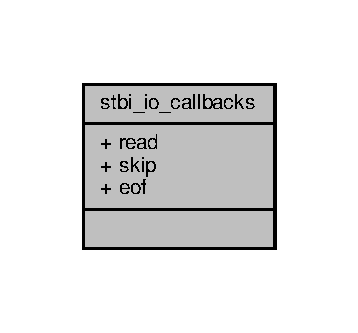
\includegraphics[width=172pt]{structstbi__io__callbacks__coll__graph}
\end{center}
\end{figure}
\subsection*{Public Attributes}
\begin{DoxyCompactItemize}
\item 
int($\ast$ \hyperlink{structstbi__io__callbacks_a623e46b3a2a019611601409926283a88}{read} )(void $\ast$user, char $\ast$data, int size)
\item 
void($\ast$ \hyperlink{structstbi__io__callbacks_a257aac5480a90a6c4b8fbe86c1b01068}{skip} )(void $\ast$user, int n)
\item 
int($\ast$ \hyperlink{structstbi__io__callbacks_a319639db2f76e715eed7a7a974136832}{eof} )(void $\ast$user)
\end{DoxyCompactItemize}


\subsection{Member Data Documentation}
\mbox{\Hypertarget{structstbi__io__callbacks_a319639db2f76e715eed7a7a974136832}\label{structstbi__io__callbacks_a319639db2f76e715eed7a7a974136832}} 
\index{stbi\+\_\+io\+\_\+callbacks@{stbi\+\_\+io\+\_\+callbacks}!eof@{eof}}
\index{eof@{eof}!stbi\+\_\+io\+\_\+callbacks@{stbi\+\_\+io\+\_\+callbacks}}
\subsubsection{\texorpdfstring{eof}{eof}}
{\footnotesize\ttfamily int($\ast$ stbi\+\_\+io\+\_\+callbacks\+::eof) (void $\ast$user)}

\mbox{\Hypertarget{structstbi__io__callbacks_a623e46b3a2a019611601409926283a88}\label{structstbi__io__callbacks_a623e46b3a2a019611601409926283a88}} 
\index{stbi\+\_\+io\+\_\+callbacks@{stbi\+\_\+io\+\_\+callbacks}!read@{read}}
\index{read@{read}!stbi\+\_\+io\+\_\+callbacks@{stbi\+\_\+io\+\_\+callbacks}}
\subsubsection{\texorpdfstring{read}{read}}
{\footnotesize\ttfamily int($\ast$ stbi\+\_\+io\+\_\+callbacks\+::read) (void $\ast$user, char $\ast$data, int size)}

\mbox{\Hypertarget{structstbi__io__callbacks_a257aac5480a90a6c4b8fbe86c1b01068}\label{structstbi__io__callbacks_a257aac5480a90a6c4b8fbe86c1b01068}} 
\index{stbi\+\_\+io\+\_\+callbacks@{stbi\+\_\+io\+\_\+callbacks}!skip@{skip}}
\index{skip@{skip}!stbi\+\_\+io\+\_\+callbacks@{stbi\+\_\+io\+\_\+callbacks}}
\subsubsection{\texorpdfstring{skip}{skip}}
{\footnotesize\ttfamily void($\ast$ stbi\+\_\+io\+\_\+callbacks\+::skip) (void $\ast$user, int n)}



The documentation for this struct was generated from the following file\+:\begin{DoxyCompactItemize}
\item 
/mnt/hdd/\+C0de/smart\+\_\+engine/include/\hyperlink{stb__image_8h}{stb\+\_\+image.\+h}\end{DoxyCompactItemize}

\hypertarget{classTextRenderer}{}\section{Text\+Renderer Class Reference}
\label{classTextRenderer}\index{Text\+Renderer@{Text\+Renderer}}


{\ttfamily \#include $<$text\+\_\+renderer.\+h$>$}



Collaboration diagram for Text\+Renderer\+:
\nopagebreak
\begin{figure}[H]
\begin{center}
\leavevmode
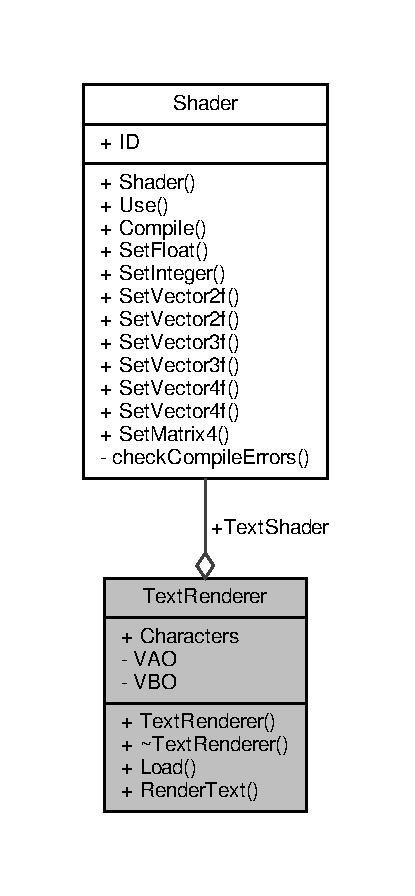
\includegraphics[width=199pt]{classTextRenderer__coll__graph}
\end{center}
\end{figure}
\subsection*{Public Member Functions}
\begin{DoxyCompactItemize}
\item 
\hyperlink{classTextRenderer_ac87978b0da75711662f6627190d5332a}{Text\+Renderer} (unsigned int width, unsigned int height)
\item 
\hyperlink{classTextRenderer_a7087505bdc31e41416408c27fe029f20}{$\sim$\+Text\+Renderer} ()
\item 
void \hyperlink{classTextRenderer_addf75e2c1eede12f9fcc465e83cec2d9}{Load} (std\+::string font, unsigned int font\+Size)
\item 
void \hyperlink{classTextRenderer_a2a206340f4c1c250bd79ebe3c7362135}{Render\+Text} (std\+::string text, float x, float y, float scale, glm\+::mat4 matrix, glm\+::vec3 color=glm\+::vec3(1.\+0f))
\end{DoxyCompactItemize}
\subsection*{Public Attributes}
\begin{DoxyCompactItemize}
\item 
std\+::map$<$ char, \hyperlink{structCharacter}{Character} $>$ \hyperlink{classTextRenderer_af7bc364007cd449284e88024c59722ba}{Characters}
\item 
\hyperlink{classShader}{Shader} $\ast$ \hyperlink{classTextRenderer_a6faaf96f0f68a45b788a8afdd3847423}{Text\+Shader}
\end{DoxyCompactItemize}
\subsection*{Private Attributes}
\begin{DoxyCompactItemize}
\item 
unsigned int \hyperlink{classTextRenderer_a7fb9e3a97f3e8438907bdde62d99bb6f}{V\+AO}
\item 
unsigned int \hyperlink{classTextRenderer_adcc1ce916e977bb17cc008f820e69b18}{V\+BO}
\end{DoxyCompactItemize}


\subsection{Constructor \& Destructor Documentation}
\mbox{\Hypertarget{classTextRenderer_ac87978b0da75711662f6627190d5332a}\label{classTextRenderer_ac87978b0da75711662f6627190d5332a}} 
\index{Text\+Renderer@{Text\+Renderer}!Text\+Renderer@{Text\+Renderer}}
\index{Text\+Renderer@{Text\+Renderer}!Text\+Renderer@{Text\+Renderer}}
\subsubsection{\texorpdfstring{Text\+Renderer()}{TextRenderer()}}
{\footnotesize\ttfamily Text\+Renderer\+::\+Text\+Renderer (\begin{DoxyParamCaption}\item[{unsigned int}]{width,  }\item[{unsigned int}]{height }\end{DoxyParamCaption})}

\mbox{\Hypertarget{classTextRenderer_a7087505bdc31e41416408c27fe029f20}\label{classTextRenderer_a7087505bdc31e41416408c27fe029f20}} 
\index{Text\+Renderer@{Text\+Renderer}!````~Text\+Renderer@{$\sim$\+Text\+Renderer}}
\index{````~Text\+Renderer@{$\sim$\+Text\+Renderer}!Text\+Renderer@{Text\+Renderer}}
\subsubsection{\texorpdfstring{$\sim$\+Text\+Renderer()}{~TextRenderer()}}
{\footnotesize\ttfamily Text\+Renderer\+::$\sim$\+Text\+Renderer (\begin{DoxyParamCaption}{ }\end{DoxyParamCaption})\hspace{0.3cm}{\ttfamily [inline]}}



\subsection{Member Function Documentation}
\mbox{\Hypertarget{classTextRenderer_addf75e2c1eede12f9fcc465e83cec2d9}\label{classTextRenderer_addf75e2c1eede12f9fcc465e83cec2d9}} 
\index{Text\+Renderer@{Text\+Renderer}!Load@{Load}}
\index{Load@{Load}!Text\+Renderer@{Text\+Renderer}}
\subsubsection{\texorpdfstring{Load()}{Load()}}
{\footnotesize\ttfamily void Text\+Renderer\+::\+Load (\begin{DoxyParamCaption}\item[{std\+::string}]{font,  }\item[{unsigned int}]{font\+Size }\end{DoxyParamCaption})}

\mbox{\Hypertarget{classTextRenderer_a2a206340f4c1c250bd79ebe3c7362135}\label{classTextRenderer_a2a206340f4c1c250bd79ebe3c7362135}} 
\index{Text\+Renderer@{Text\+Renderer}!Render\+Text@{Render\+Text}}
\index{Render\+Text@{Render\+Text}!Text\+Renderer@{Text\+Renderer}}
\subsubsection{\texorpdfstring{Render\+Text()}{RenderText()}}
{\footnotesize\ttfamily void Text\+Renderer\+::\+Render\+Text (\begin{DoxyParamCaption}\item[{std\+::string}]{text,  }\item[{float}]{x,  }\item[{float}]{y,  }\item[{float}]{scale,  }\item[{glm\+::mat4}]{matrix,  }\item[{glm\+::vec3}]{color = {\ttfamily glm\+:\+:vec3(1.0f)} }\end{DoxyParamCaption})}



\subsection{Member Data Documentation}
\mbox{\Hypertarget{classTextRenderer_af7bc364007cd449284e88024c59722ba}\label{classTextRenderer_af7bc364007cd449284e88024c59722ba}} 
\index{Text\+Renderer@{Text\+Renderer}!Characters@{Characters}}
\index{Characters@{Characters}!Text\+Renderer@{Text\+Renderer}}
\subsubsection{\texorpdfstring{Characters}{Characters}}
{\footnotesize\ttfamily std\+::map$<$char, \hyperlink{structCharacter}{Character}$>$ Text\+Renderer\+::\+Characters}

\mbox{\Hypertarget{classTextRenderer_a6faaf96f0f68a45b788a8afdd3847423}\label{classTextRenderer_a6faaf96f0f68a45b788a8afdd3847423}} 
\index{Text\+Renderer@{Text\+Renderer}!Text\+Shader@{Text\+Shader}}
\index{Text\+Shader@{Text\+Shader}!Text\+Renderer@{Text\+Renderer}}
\subsubsection{\texorpdfstring{Text\+Shader}{TextShader}}
{\footnotesize\ttfamily \hyperlink{classShader}{Shader}$\ast$ Text\+Renderer\+::\+Text\+Shader}

\mbox{\Hypertarget{classTextRenderer_a7fb9e3a97f3e8438907bdde62d99bb6f}\label{classTextRenderer_a7fb9e3a97f3e8438907bdde62d99bb6f}} 
\index{Text\+Renderer@{Text\+Renderer}!V\+AO@{V\+AO}}
\index{V\+AO@{V\+AO}!Text\+Renderer@{Text\+Renderer}}
\subsubsection{\texorpdfstring{V\+AO}{VAO}}
{\footnotesize\ttfamily unsigned int Text\+Renderer\+::\+V\+AO\hspace{0.3cm}{\ttfamily [private]}}

\mbox{\Hypertarget{classTextRenderer_adcc1ce916e977bb17cc008f820e69b18}\label{classTextRenderer_adcc1ce916e977bb17cc008f820e69b18}} 
\index{Text\+Renderer@{Text\+Renderer}!V\+BO@{V\+BO}}
\index{V\+BO@{V\+BO}!Text\+Renderer@{Text\+Renderer}}
\subsubsection{\texorpdfstring{V\+BO}{VBO}}
{\footnotesize\ttfamily unsigned int Text\+Renderer\+::\+V\+BO\hspace{0.3cm}{\ttfamily [private]}}



The documentation for this class was generated from the following files\+:\begin{DoxyCompactItemize}
\item 
/mnt/hdd/\+C0de/smart\+\_\+engine/include/\hyperlink{text__renderer_8h}{text\+\_\+renderer.\+h}\item 
/mnt/hdd/\+C0de/smart\+\_\+engine/src/\hyperlink{text__renderer_8cpp}{text\+\_\+renderer.\+cpp}\end{DoxyCompactItemize}

\hypertarget{classTexture2D}{}\section{Texture2D Class Reference}
\label{classTexture2D}\index{Texture2D@{Texture2D}}


{\ttfamily \#include $<$texture.\+h$>$}



Inheritance diagram for Texture2D\+:
\nopagebreak
\begin{figure}[H]
\begin{center}
\leavevmode
\includegraphics[height=550pt]{classTexture2D__inherit__graph}
\end{center}
\end{figure}


Collaboration diagram for Texture2D\+:
\nopagebreak
\begin{figure}[H]
\begin{center}
\leavevmode
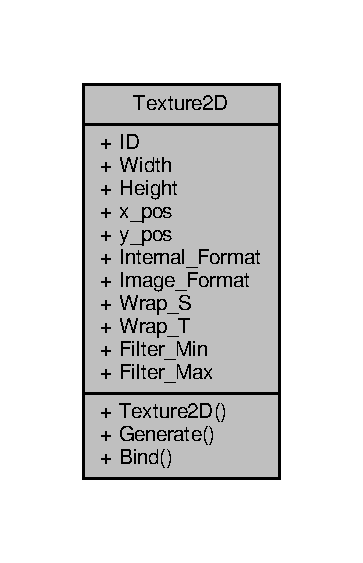
\includegraphics[width=174pt]{classTexture2D__coll__graph}
\end{center}
\end{figure}
\subsection*{Public Member Functions}
\begin{DoxyCompactItemize}
\item 
\hyperlink{classTexture2D_ab62c7c5172a4800b4629cd475147819d}{Texture2D} ()
\item 
void \hyperlink{classTexture2D_a29768bc9e468322d8b6b86374890c2cc}{Generate} (unsigned int width, unsigned int height, unsigned char $\ast$data)
\item 
void \hyperlink{classTexture2D_a97cc1e27512b8f520a59473e6657d7d9}{Bind} () const
\end{DoxyCompactItemize}
\subsection*{Public Attributes}
\begin{DoxyCompactItemize}
\item 
unsigned int \hyperlink{classTexture2D_ac5639377a74a227b0b2369c159dc6d46}{ID}
\item 
unsigned int \hyperlink{classTexture2D_a558054990d7e668b9df119713922fa53}{Width}
\item 
unsigned int \hyperlink{classTexture2D_a640768f0078c4c96c7fb80150c548201}{Height}
\item 
float \hyperlink{classTexture2D_a5d7a290a99c99a921e0bbed6e8b529f8}{x\+\_\+pos}
\item 
float \hyperlink{classTexture2D_aeb7e15444821c2bb23d5026ca4430e58}{y\+\_\+pos}
\item 
unsigned int \hyperlink{classTexture2D_a9491c93c156e1a33a4c8d0116aedfffa}{Internal\+\_\+\+Format}
\item 
unsigned int \hyperlink{classTexture2D_a9e4a5f6606148ac84be4c8c096553808}{Image\+\_\+\+Format}
\item 
unsigned int \hyperlink{classTexture2D_a95dc93c0a76a5d30d7b1fade841a58df}{Wrap\+\_\+S}
\item 
unsigned int \hyperlink{classTexture2D_a80e39ea4cf66bbed444cdf135afffb92}{Wrap\+\_\+T}
\item 
unsigned int \hyperlink{classTexture2D_a09545dae0e8b68db570506e3aae8e99b}{Filter\+\_\+\+Min}
\item 
unsigned int \hyperlink{classTexture2D_ac4c49410570a07a5b7fd0ec4a18ab646}{Filter\+\_\+\+Max}
\end{DoxyCompactItemize}


\subsection{Constructor \& Destructor Documentation}
\mbox{\Hypertarget{classTexture2D_ab62c7c5172a4800b4629cd475147819d}\label{classTexture2D_ab62c7c5172a4800b4629cd475147819d}} 
\index{Texture2D@{Texture2D}!Texture2D@{Texture2D}}
\index{Texture2D@{Texture2D}!Texture2D@{Texture2D}}
\subsubsection{\texorpdfstring{Texture2\+D()}{Texture2D()}}
{\footnotesize\ttfamily Texture2\+D\+::\+Texture2D (\begin{DoxyParamCaption}{ }\end{DoxyParamCaption})}



\subsection{Member Function Documentation}
\mbox{\Hypertarget{classTexture2D_a97cc1e27512b8f520a59473e6657d7d9}\label{classTexture2D_a97cc1e27512b8f520a59473e6657d7d9}} 
\index{Texture2D@{Texture2D}!Bind@{Bind}}
\index{Bind@{Bind}!Texture2D@{Texture2D}}
\subsubsection{\texorpdfstring{Bind()}{Bind()}}
{\footnotesize\ttfamily void Texture2\+D\+::\+Bind (\begin{DoxyParamCaption}{ }\end{DoxyParamCaption}) const}

\mbox{\Hypertarget{classTexture2D_a29768bc9e468322d8b6b86374890c2cc}\label{classTexture2D_a29768bc9e468322d8b6b86374890c2cc}} 
\index{Texture2D@{Texture2D}!Generate@{Generate}}
\index{Generate@{Generate}!Texture2D@{Texture2D}}
\subsubsection{\texorpdfstring{Generate()}{Generate()}}
{\footnotesize\ttfamily void Texture2\+D\+::\+Generate (\begin{DoxyParamCaption}\item[{unsigned int}]{width,  }\item[{unsigned int}]{height,  }\item[{unsigned char $\ast$}]{data }\end{DoxyParamCaption})}



\subsection{Member Data Documentation}
\mbox{\Hypertarget{classTexture2D_ac4c49410570a07a5b7fd0ec4a18ab646}\label{classTexture2D_ac4c49410570a07a5b7fd0ec4a18ab646}} 
\index{Texture2D@{Texture2D}!Filter\+\_\+\+Max@{Filter\+\_\+\+Max}}
\index{Filter\+\_\+\+Max@{Filter\+\_\+\+Max}!Texture2D@{Texture2D}}
\subsubsection{\texorpdfstring{Filter\+\_\+\+Max}{Filter\_Max}}
{\footnotesize\ttfamily unsigned int Texture2\+D\+::\+Filter\+\_\+\+Max}

\mbox{\Hypertarget{classTexture2D_a09545dae0e8b68db570506e3aae8e99b}\label{classTexture2D_a09545dae0e8b68db570506e3aae8e99b}} 
\index{Texture2D@{Texture2D}!Filter\+\_\+\+Min@{Filter\+\_\+\+Min}}
\index{Filter\+\_\+\+Min@{Filter\+\_\+\+Min}!Texture2D@{Texture2D}}
\subsubsection{\texorpdfstring{Filter\+\_\+\+Min}{Filter\_Min}}
{\footnotesize\ttfamily unsigned int Texture2\+D\+::\+Filter\+\_\+\+Min}

\mbox{\Hypertarget{classTexture2D_a640768f0078c4c96c7fb80150c548201}\label{classTexture2D_a640768f0078c4c96c7fb80150c548201}} 
\index{Texture2D@{Texture2D}!Height@{Height}}
\index{Height@{Height}!Texture2D@{Texture2D}}
\subsubsection{\texorpdfstring{Height}{Height}}
{\footnotesize\ttfamily unsigned int Texture2\+D\+::\+Height}

\mbox{\Hypertarget{classTexture2D_ac5639377a74a227b0b2369c159dc6d46}\label{classTexture2D_ac5639377a74a227b0b2369c159dc6d46}} 
\index{Texture2D@{Texture2D}!ID@{ID}}
\index{ID@{ID}!Texture2D@{Texture2D}}
\subsubsection{\texorpdfstring{ID}{ID}}
{\footnotesize\ttfamily unsigned int Texture2\+D\+::\+ID}

\mbox{\Hypertarget{classTexture2D_a9e4a5f6606148ac84be4c8c096553808}\label{classTexture2D_a9e4a5f6606148ac84be4c8c096553808}} 
\index{Texture2D@{Texture2D}!Image\+\_\+\+Format@{Image\+\_\+\+Format}}
\index{Image\+\_\+\+Format@{Image\+\_\+\+Format}!Texture2D@{Texture2D}}
\subsubsection{\texorpdfstring{Image\+\_\+\+Format}{Image\_Format}}
{\footnotesize\ttfamily unsigned int Texture2\+D\+::\+Image\+\_\+\+Format}

\mbox{\Hypertarget{classTexture2D_a9491c93c156e1a33a4c8d0116aedfffa}\label{classTexture2D_a9491c93c156e1a33a4c8d0116aedfffa}} 
\index{Texture2D@{Texture2D}!Internal\+\_\+\+Format@{Internal\+\_\+\+Format}}
\index{Internal\+\_\+\+Format@{Internal\+\_\+\+Format}!Texture2D@{Texture2D}}
\subsubsection{\texorpdfstring{Internal\+\_\+\+Format}{Internal\_Format}}
{\footnotesize\ttfamily unsigned int Texture2\+D\+::\+Internal\+\_\+\+Format}

\mbox{\Hypertarget{classTexture2D_a558054990d7e668b9df119713922fa53}\label{classTexture2D_a558054990d7e668b9df119713922fa53}} 
\index{Texture2D@{Texture2D}!Width@{Width}}
\index{Width@{Width}!Texture2D@{Texture2D}}
\subsubsection{\texorpdfstring{Width}{Width}}
{\footnotesize\ttfamily unsigned int Texture2\+D\+::\+Width}

\mbox{\Hypertarget{classTexture2D_a95dc93c0a76a5d30d7b1fade841a58df}\label{classTexture2D_a95dc93c0a76a5d30d7b1fade841a58df}} 
\index{Texture2D@{Texture2D}!Wrap\+\_\+S@{Wrap\+\_\+S}}
\index{Wrap\+\_\+S@{Wrap\+\_\+S}!Texture2D@{Texture2D}}
\subsubsection{\texorpdfstring{Wrap\+\_\+S}{Wrap\_S}}
{\footnotesize\ttfamily unsigned int Texture2\+D\+::\+Wrap\+\_\+S}

\mbox{\Hypertarget{classTexture2D_a80e39ea4cf66bbed444cdf135afffb92}\label{classTexture2D_a80e39ea4cf66bbed444cdf135afffb92}} 
\index{Texture2D@{Texture2D}!Wrap\+\_\+T@{Wrap\+\_\+T}}
\index{Wrap\+\_\+T@{Wrap\+\_\+T}!Texture2D@{Texture2D}}
\subsubsection{\texorpdfstring{Wrap\+\_\+T}{Wrap\_T}}
{\footnotesize\ttfamily unsigned int Texture2\+D\+::\+Wrap\+\_\+T}

\mbox{\Hypertarget{classTexture2D_a5d7a290a99c99a921e0bbed6e8b529f8}\label{classTexture2D_a5d7a290a99c99a921e0bbed6e8b529f8}} 
\index{Texture2D@{Texture2D}!x\+\_\+pos@{x\+\_\+pos}}
\index{x\+\_\+pos@{x\+\_\+pos}!Texture2D@{Texture2D}}
\subsubsection{\texorpdfstring{x\+\_\+pos}{x\_pos}}
{\footnotesize\ttfamily float Texture2\+D\+::x\+\_\+pos}

\mbox{\Hypertarget{classTexture2D_aeb7e15444821c2bb23d5026ca4430e58}\label{classTexture2D_aeb7e15444821c2bb23d5026ca4430e58}} 
\index{Texture2D@{Texture2D}!y\+\_\+pos@{y\+\_\+pos}}
\index{y\+\_\+pos@{y\+\_\+pos}!Texture2D@{Texture2D}}
\subsubsection{\texorpdfstring{y\+\_\+pos}{y\_pos}}
{\footnotesize\ttfamily float Texture2\+D\+::y\+\_\+pos}



The documentation for this class was generated from the following files\+:\begin{DoxyCompactItemize}
\item 
/mnt/hdd/\+C0de/smart\+\_\+engine/include/\hyperlink{texture_8h}{texture.\+h}\item 
/mnt/hdd/\+C0de/smart\+\_\+engine/src/\hyperlink{texture_8cpp}{texture.\+cpp}\end{DoxyCompactItemize}

\chapter{File Documentation}
\hypertarget{entity_8h}{}\section{/mnt/hdd/\+C0de/smart\+\_\+engine/include/entity.h File Reference}
\label{entity_8h}\index{/mnt/hdd/\+C0de/smart\+\_\+engine/include/entity.\+h@{/mnt/hdd/\+C0de/smart\+\_\+engine/include/entity.\+h}}
{\ttfamily \#include \char`\"{}texture.\+h\char`\"{}}\newline
{\ttfamily \#include $<$box2d/box2d.\+h$>$}\newline
{\ttfamily \#include $<$iostream$>$}\newline
{\ttfamily \#include $<$memory$>$}\newline
{\ttfamily \#include \char`\"{}resource\+\_\+manager.\+h\char`\"{}}\newline
{\ttfamily \#include $<$glm/glm.\+hpp$>$}\newline
Include dependency graph for entity.\+h\+:
\nopagebreak
\begin{figure}[H]
\begin{center}
\leavevmode
\includegraphics[width=350pt]{entity_8h__incl}
\end{center}
\end{figure}
This graph shows which files directly or indirectly include this file\+:
\nopagebreak
\begin{figure}[H]
\begin{center}
\leavevmode
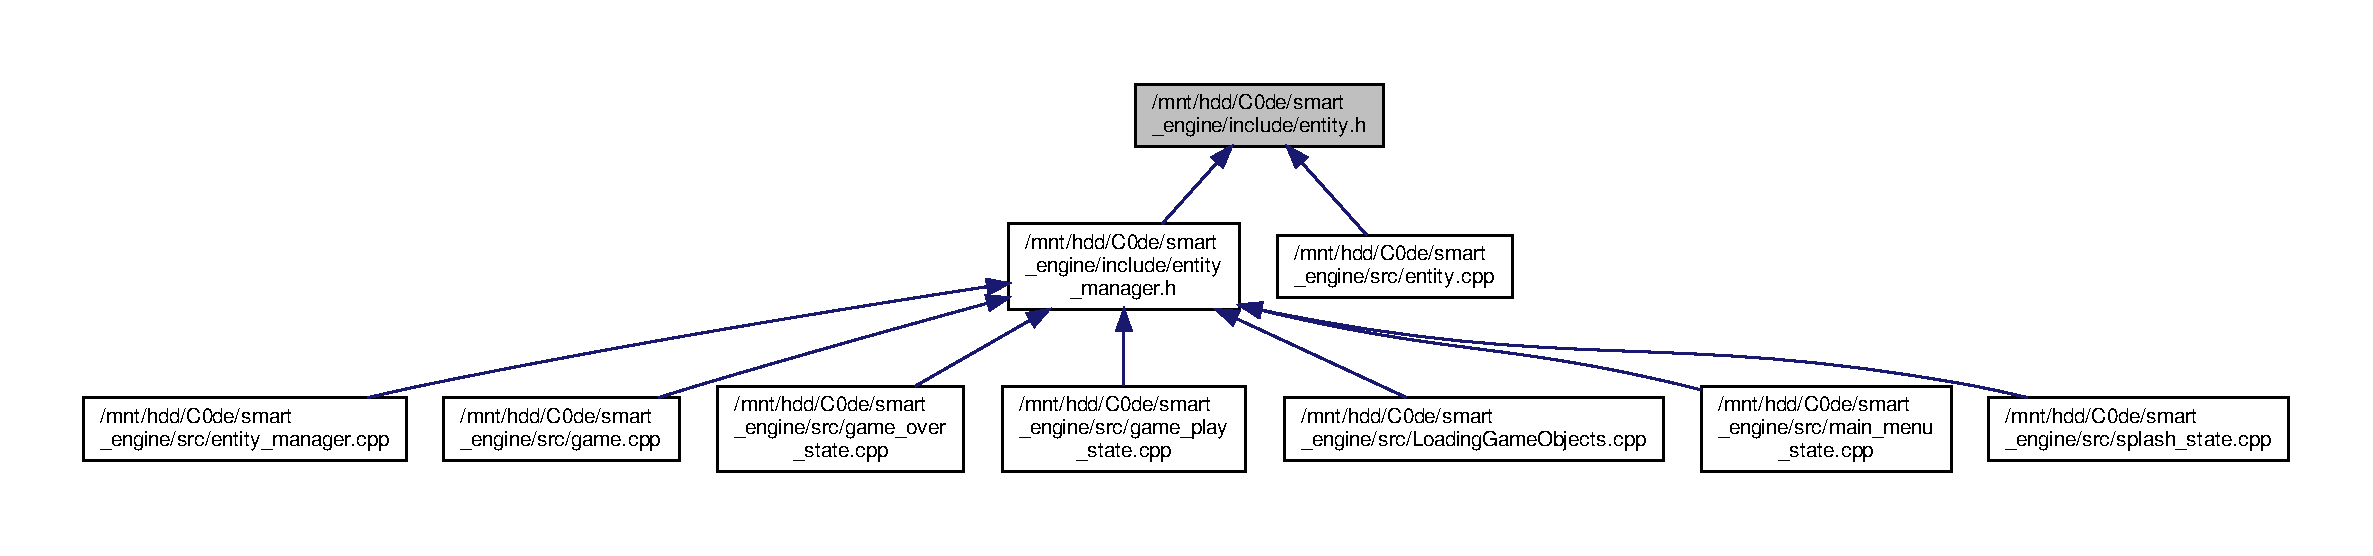
\includegraphics[width=350pt]{entity_8h__dep__incl}
\end{center}
\end{figure}
\subsection*{Classes}
\begin{DoxyCompactItemize}
\item 
struct \hyperlink{structb0x__2d__SHAPES}{b0x\+\_\+2d\+\_\+\+S\+H\+A\+P\+ES}
\item 
class \hyperlink{classEntity}{Entity}
\end{DoxyCompactItemize}

\hypertarget{entity__manager_8h}{}\section{/mnt/hdd/\+C0de/\+Engines/\+S\+F\+M\+L/\+S\+F\+M\+L\+\_\+\+Engine/include/entity\+\_\+manager.h File Reference}
\label{entity__manager_8h}\index{/mnt/hdd/\+C0de/\+Engines/\+S\+F\+M\+L/\+S\+F\+M\+L\+\_\+\+Engine/include/entity\+\_\+manager.\+h@{/mnt/hdd/\+C0de/\+Engines/\+S\+F\+M\+L/\+S\+F\+M\+L\+\_\+\+Engine/include/entity\+\_\+manager.\+h}}
{\ttfamily \#include $<$unordered\+\_\+map$>$}\newline
{\ttfamily \#include $<$vector$>$}\newline
{\ttfamily \#include $<$box2d/box2d.\+h$>$}\newline
{\ttfamily \#include \char`\"{}entity.\+h\char`\"{}}\newline
Include dependency graph for entity\+\_\+manager.\+h\+:
\nopagebreak
\begin{figure}[H]
\begin{center}
\leavevmode
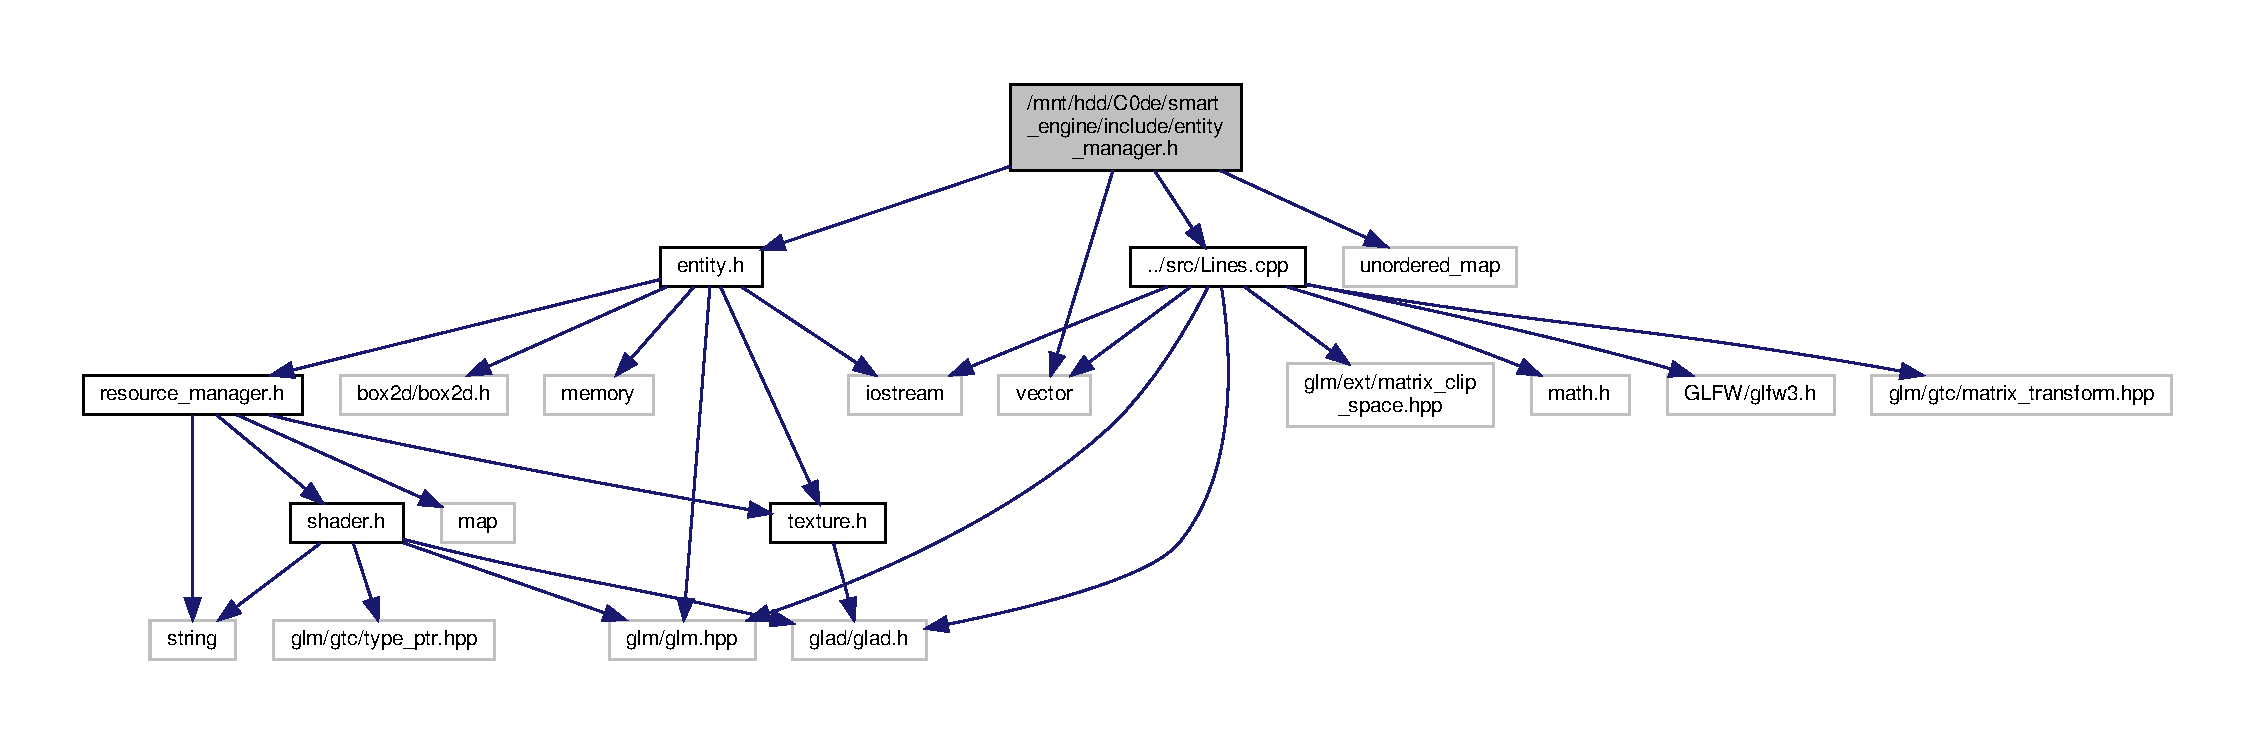
\includegraphics[width=350pt]{entity__manager_8h__incl}
\end{center}
\end{figure}
This graph shows which files directly or indirectly include this file\+:
\nopagebreak
\begin{figure}[H]
\begin{center}
\leavevmode
\includegraphics[width=350pt]{entity__manager_8h__dep__incl}
\end{center}
\end{figure}
\subsection*{Classes}
\begin{DoxyCompactItemize}
\item 
class \hyperlink{classSekander_1_1EntityManager}{Sekander\+::\+Entity\+Manager}
\end{DoxyCompactItemize}
\subsection*{Namespaces}
\begin{DoxyCompactItemize}
\item 
 \hyperlink{namespaceSekander}{Sekander}
\end{DoxyCompactItemize}
\subsection*{Enumerations}
\begin{DoxyCompactItemize}
\item 
enum \hyperlink{namespaceSekander_aed8eb219f4685b29738464e9f32c5d94}{Sekander\+::shape\+\_\+options} \{ \hyperlink{namespaceSekander_aed8eb219f4685b29738464e9f32c5d94ae1827bea553b36ce0bbc7cddd6c57621}{Sekander\+::\+Square} = 1, 
\hyperlink{namespaceSekander_aed8eb219f4685b29738464e9f32c5d94acafcba9574f3415e8e9f6f194a6cb869}{Sekander\+::\+Circle} = 2
 \}
\end{DoxyCompactItemize}

\hypertarget{game_8h}{}\section{/mnt/hdd/\+C0de/smart\+\_\+engine/include/game.h File Reference}
\label{game_8h}\index{/mnt/hdd/\+C0de/smart\+\_\+engine/include/game.\+h@{/mnt/hdd/\+C0de/smart\+\_\+engine/include/game.\+h}}
{\ttfamily \#include $<$memory$>$}\newline
{\ttfamily \#include $<$iostream$>$}\newline
{\ttfamily \#include \char`\"{}Orthographic\+\_\+camera.\+h\char`\"{}}\newline
{\ttfamily \#include \char`\"{}state\+\_\+machine.\+h\char`\"{}}\newline
{\ttfamily \#include \char`\"{}G\+L\+F\+W/glfw3.\+h\char`\"{}}\newline
Include dependency graph for game.\+h\+:
\nopagebreak
\begin{figure}[H]
\begin{center}
\leavevmode
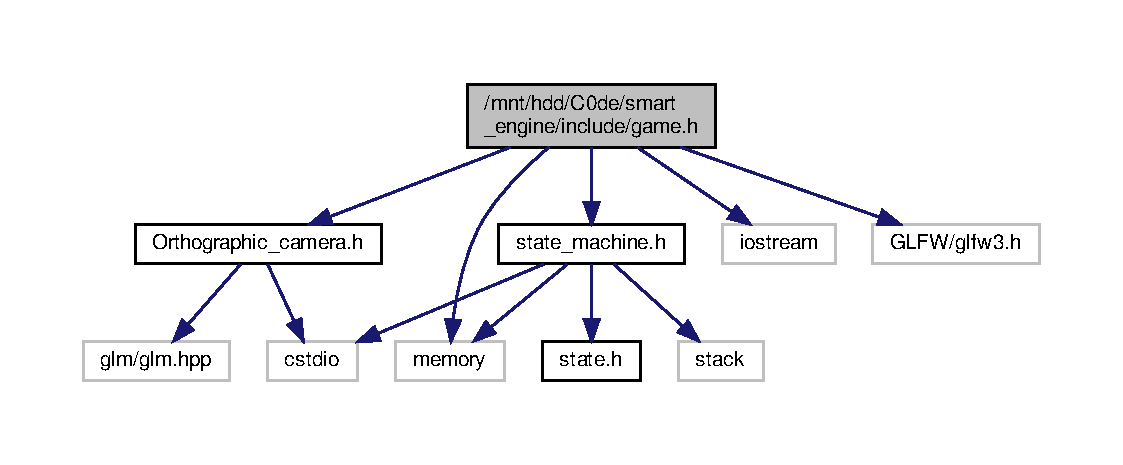
\includegraphics[width=350pt]{game_8h__incl}
\end{center}
\end{figure}
This graph shows which files directly or indirectly include this file\+:
\nopagebreak
\begin{figure}[H]
\begin{center}
\leavevmode
\includegraphics[width=350pt]{game_8h__dep__incl}
\end{center}
\end{figure}
\subsection*{Classes}
\begin{DoxyCompactItemize}
\item 
struct \hyperlink{structGameData}{Game\+Data}
\item 
class \hyperlink{classGame}{Game}
\end{DoxyCompactItemize}
\subsection*{Typedefs}
\begin{DoxyCompactItemize}
\item 
using \hyperlink{game_8h_a513c9dd465a0df41dbb4daf40cc717c2}{Game\+Data\+Ref} = std\+::shared\+\_\+ptr$<$ \hyperlink{structGameData}{Game\+Data} $>$
\end{DoxyCompactItemize}


\subsection{Typedef Documentation}
\mbox{\Hypertarget{game_8h_a513c9dd465a0df41dbb4daf40cc717c2}\label{game_8h_a513c9dd465a0df41dbb4daf40cc717c2}} 
\index{game.\+h@{game.\+h}!Game\+Data\+Ref@{Game\+Data\+Ref}}
\index{Game\+Data\+Ref@{Game\+Data\+Ref}!game.\+h@{game.\+h}}
\subsubsection{\texorpdfstring{Game\+Data\+Ref}{GameDataRef}}
{\footnotesize\ttfamily using \hyperlink{game_8h_a513c9dd465a0df41dbb4daf40cc717c2}{Game\+Data\+Ref} =  std\+::shared\+\_\+ptr$<$\hyperlink{structGameData}{Game\+Data}$>$}


\hypertarget{game__over__state_8h}{}\section{/mnt/hdd/\+C0de/smart\+\_\+engine/include/game\+\_\+over\+\_\+state.h File Reference}
\label{game__over__state_8h}\index{/mnt/hdd/\+C0de/smart\+\_\+engine/include/game\+\_\+over\+\_\+state.\+h@{/mnt/hdd/\+C0de/smart\+\_\+engine/include/game\+\_\+over\+\_\+state.\+h}}
{\ttfamily \#include \char`\"{}state.\+h\char`\"{}}\newline
{\ttfamily \#include \char`\"{}game.\+h\char`\"{}}\newline
Include dependency graph for game\+\_\+over\+\_\+state.\+h\+:
\nopagebreak
\begin{figure}[H]
\begin{center}
\leavevmode
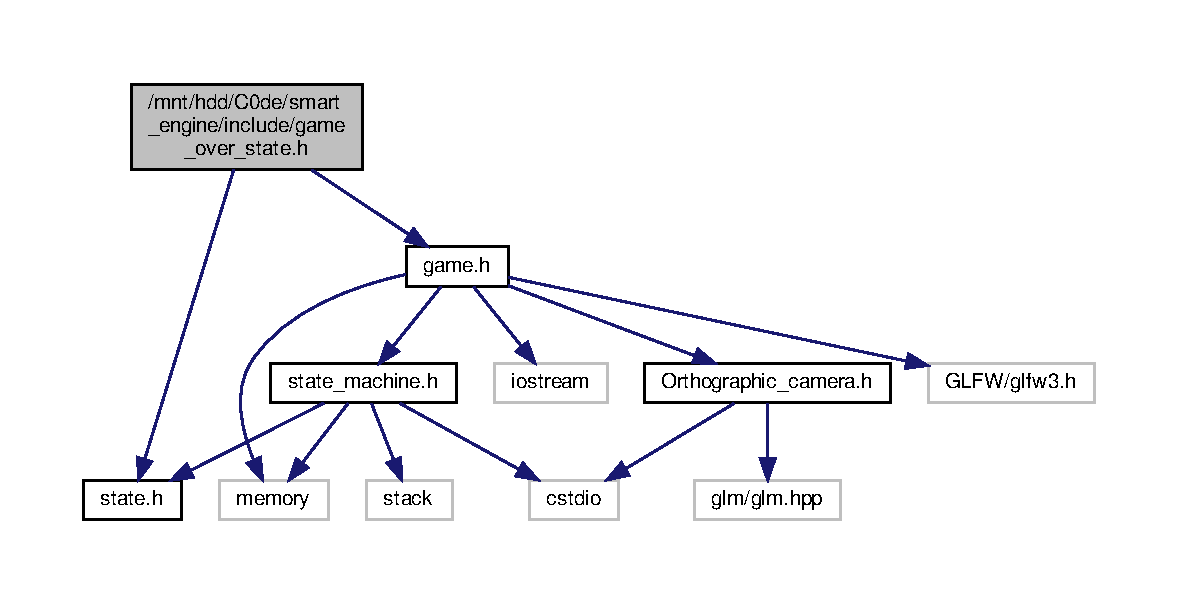
\includegraphics[width=350pt]{game__over__state_8h__incl}
\end{center}
\end{figure}
This graph shows which files directly or indirectly include this file\+:
\nopagebreak
\begin{figure}[H]
\begin{center}
\leavevmode
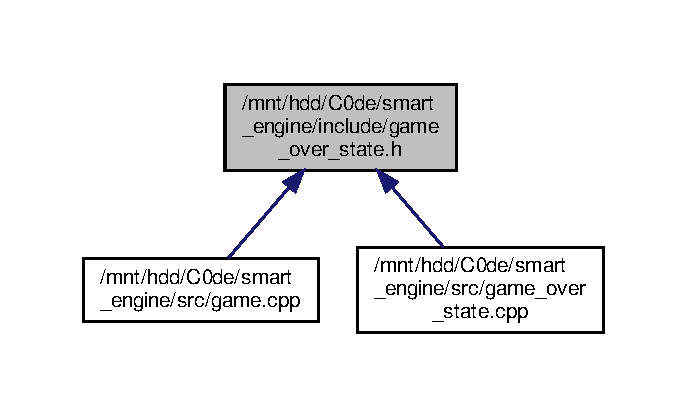
\includegraphics[width=330pt]{game__over__state_8h__dep__incl}
\end{center}
\end{figure}
\subsection*{Classes}
\begin{DoxyCompactItemize}
\item 
class \hyperlink{classGameOverState}{Game\+Over\+State}
\end{DoxyCompactItemize}

\hypertarget{game__play__state_8h}{}\section{/mnt/hdd/\+C0de/smart\+\_\+engine/include/game\+\_\+play\+\_\+state.h File Reference}
\label{game__play__state_8h}\index{/mnt/hdd/\+C0de/smart\+\_\+engine/include/game\+\_\+play\+\_\+state.\+h@{/mnt/hdd/\+C0de/smart\+\_\+engine/include/game\+\_\+play\+\_\+state.\+h}}
{\ttfamily \#include \char`\"{}state.\+h\char`\"{}}\newline
{\ttfamily \#include \char`\"{}game.\+h\char`\"{}}\newline
Include dependency graph for game\+\_\+play\+\_\+state.\+h\+:
\nopagebreak
\begin{figure}[H]
\begin{center}
\leavevmode
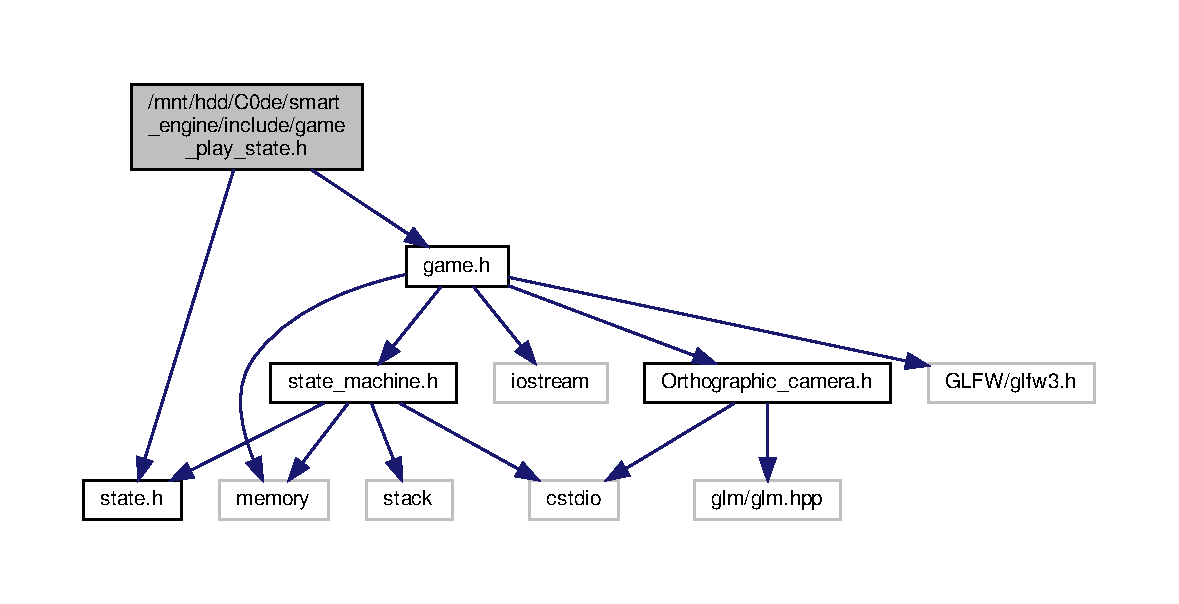
\includegraphics[width=350pt]{game__play__state_8h__incl}
\end{center}
\end{figure}
This graph shows which files directly or indirectly include this file\+:
\nopagebreak
\begin{figure}[H]
\begin{center}
\leavevmode
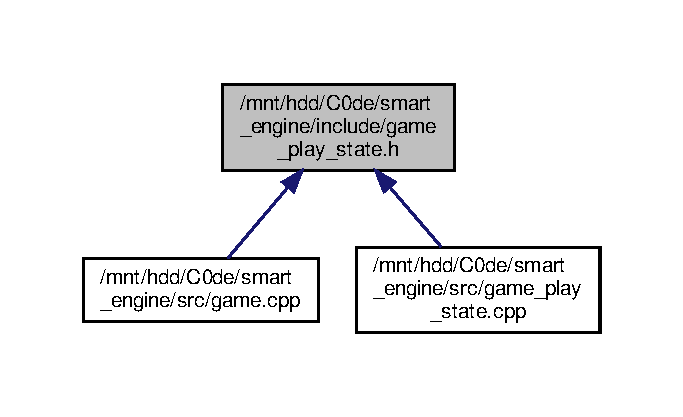
\includegraphics[width=328pt]{game__play__state_8h__dep__incl}
\end{center}
\end{figure}
\subsection*{Classes}
\begin{DoxyCompactItemize}
\item 
class \hyperlink{classGamePlayState}{Game\+Play\+State}
\end{DoxyCompactItemize}

\hypertarget{game__text_8h}{}\section{/mnt/hdd/\+C0de/smart\+\_\+engine/include/game\+\_\+text.h File Reference}
\label{game__text_8h}\index{/mnt/hdd/\+C0de/smart\+\_\+engine/include/game\+\_\+text.\+h@{/mnt/hdd/\+C0de/smart\+\_\+engine/include/game\+\_\+text.\+h}}
{\ttfamily \#include $<$stdio.\+h$>$}\newline
{\ttfamily \#include $<$iostream$>$}\newline
Include dependency graph for game\+\_\+text.\+h\+:
\nopagebreak
\begin{figure}[H]
\begin{center}
\leavevmode
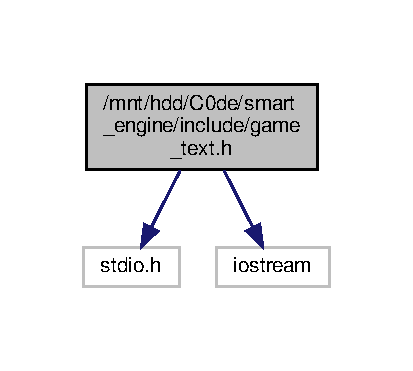
\includegraphics[width=198pt]{game__text_8h__incl}
\end{center}
\end{figure}
This graph shows which files directly or indirectly include this file\+:
\nopagebreak
\begin{figure}[H]
\begin{center}
\leavevmode
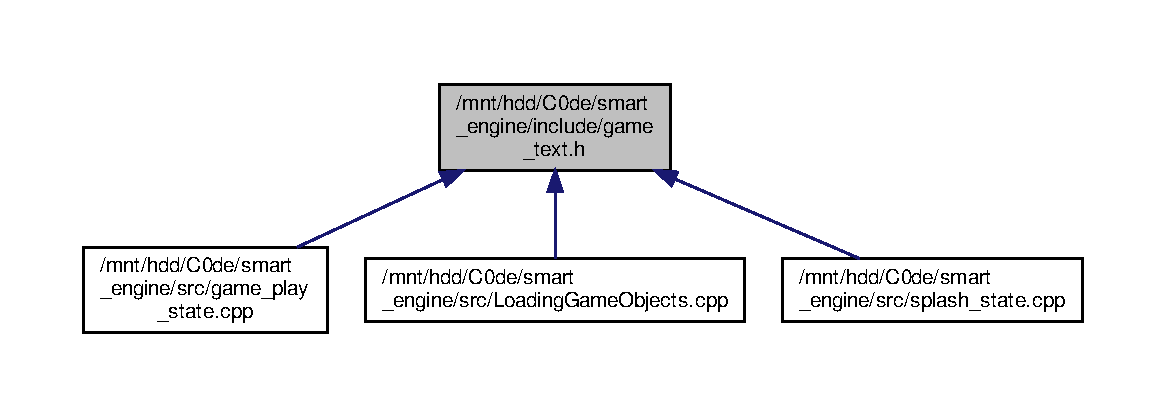
\includegraphics[width=350pt]{game__text_8h__dep__incl}
\end{center}
\end{figure}
\subsection*{Classes}
\begin{DoxyCompactItemize}
\item 
class \hyperlink{classgame__text}{game\+\_\+text}
\end{DoxyCompactItemize}

\hypertarget{gltext_8h}{}\section{/mnt/hdd/\+C0de/smart\+\_\+engine/include/gltext.h File Reference}
\label{gltext_8h}\index{/mnt/hdd/\+C0de/smart\+\_\+engine/include/gltext.\+h@{/mnt/hdd/\+C0de/smart\+\_\+engine/include/gltext.\+h}}
{\ttfamily \#include \char`\"{}G\+L/gl.\+h\char`\"{}}\newline
{\ttfamily \#include $<$stdlib.\+h$>$}\newline
{\ttfamily \#include $<$string.\+h$>$}\newline
{\ttfamily \#include $<$stdint.\+h$>$}\newline
Include dependency graph for gltext.\+h\+:
\nopagebreak
\begin{figure}[H]
\begin{center}
\leavevmode
\includegraphics[width=329pt]{gltext_8h__incl}
\end{center}
\end{figure}
\subsection*{Macros}
\begin{DoxyCompactItemize}
\item 
\#define \hyperlink{gltext_8h_a67a14251d45d84381eb6cf27fc760681}{\+\_\+\+G\+L\+T\+\_\+\+A\+S\+S\+E\+RT}(expression)
\item 
\#define \hyperlink{gltext_8h_ad09179d4634e408a46e73b1da34b5117}{\+\_\+\+G\+L\+T\+\_\+\+S\+T\+R\+I\+N\+G\+I\+FY}(str)~\#str
\item 
\#define \hyperlink{gltext_8h_afb5349d0435ad558a05d8ba4117c8d55}{\+\_\+\+G\+L\+T\+\_\+\+S\+T\+R\+I\+N\+G\+I\+F\+Y\+\_\+\+T\+O\+K\+EN}(str)~\hyperlink{gltext_8h_ad09179d4634e408a46e73b1da34b5117}{\+\_\+\+G\+L\+T\+\_\+\+S\+T\+R\+I\+N\+G\+I\+FY}(str)
\item 
\#define \hyperlink{gltext_8h_a5132f3add5f8a9b8ef9896965cf85a3b}{G\+L\+T\+\_\+\+S\+T\+R\+I\+N\+G\+I\+F\+Y\+\_\+\+V\+E\+R\+S\+I\+ON}(major,  minor,  patch)~\hyperlink{gltext_8h_ad09179d4634e408a46e73b1da34b5117}{\+\_\+\+G\+L\+T\+\_\+\+S\+T\+R\+I\+N\+G\+I\+FY}(major) \char`\"{}.\char`\"{} \hyperlink{gltext_8h_ad09179d4634e408a46e73b1da34b5117}{\+\_\+\+G\+L\+T\+\_\+\+S\+T\+R\+I\+N\+G\+I\+FY}(minor) \char`\"{}.\char`\"{} \hyperlink{gltext_8h_ad09179d4634e408a46e73b1da34b5117}{\+\_\+\+G\+L\+T\+\_\+\+S\+T\+R\+I\+N\+G\+I\+FY}(patch)
\item 
\#define \hyperlink{gltext_8h_a9c7f809d1768e5f959ad7f0ddc4938c4}{G\+L\+T\+\_\+\+N\+A\+ME}~\char`\"{}gl\+Text\char`\"{}
\item 
\#define \hyperlink{gltext_8h_a5dca984536ac85ebd293445dccfef467}{G\+L\+T\+\_\+\+V\+E\+R\+S\+I\+O\+N\+\_\+\+M\+A\+J\+OR}~1
\item 
\#define \hyperlink{gltext_8h_a55184d8a7dbeb1c821f42b5d6d72b6ba}{G\+L\+T\+\_\+\+V\+E\+R\+S\+I\+O\+N\+\_\+\+M\+I\+N\+OR}~1
\item 
\#define \hyperlink{gltext_8h_a330c7a3a1fb7be6f127b7c1df66dc979}{G\+L\+T\+\_\+\+V\+E\+R\+S\+I\+O\+N\+\_\+\+P\+A\+T\+CH}~6
\item 
\#define \hyperlink{gltext_8h_a426ab2585e41480e69776acad6e31dd4}{G\+L\+T\+\_\+\+V\+E\+R\+S\+I\+ON}~\hyperlink{gltext_8h_a5132f3add5f8a9b8ef9896965cf85a3b}{G\+L\+T\+\_\+\+S\+T\+R\+I\+N\+G\+I\+F\+Y\+\_\+\+V\+E\+R\+S\+I\+ON}(\hyperlink{gltext_8h_a5dca984536ac85ebd293445dccfef467}{G\+L\+T\+\_\+\+V\+E\+R\+S\+I\+O\+N\+\_\+\+M\+A\+J\+OR}, \hyperlink{gltext_8h_a55184d8a7dbeb1c821f42b5d6d72b6ba}{G\+L\+T\+\_\+\+V\+E\+R\+S\+I\+O\+N\+\_\+\+M\+I\+N\+OR}, \hyperlink{gltext_8h_a330c7a3a1fb7be6f127b7c1df66dc979}{G\+L\+T\+\_\+\+V\+E\+R\+S\+I\+O\+N\+\_\+\+P\+A\+T\+CH})
\item 
\#define \hyperlink{gltext_8h_a4f9d36f0b9a091c6a7145b420b148274}{G\+L\+T\+\_\+\+N\+A\+M\+E\+\_\+\+V\+E\+R\+S\+I\+ON}~\hyperlink{gltext_8h_a9c7f809d1768e5f959ad7f0ddc4938c4}{G\+L\+T\+\_\+\+N\+A\+ME} \char`\"{} \char`\"{} \hyperlink{gltext_8h_a426ab2585e41480e69776acad6e31dd4}{G\+L\+T\+\_\+\+V\+E\+R\+S\+I\+ON}
\item 
\#define \hyperlink{gltext_8h_a77689b1302bd5028dd47bb34ab1f41b8}{G\+L\+T\+\_\+\+N\+U\+LL}~0
\item 
\#define \hyperlink{gltext_8h_a8d280924462a5dbe00c2c632579e7b28}{G\+L\+T\+\_\+\+N\+U\+L\+L\+\_\+\+H\+A\+N\+D\+LE}~0
\item 
\#define \hyperlink{gltext_8h_a62344ecade473e517e772c1b46ac3b89}{G\+L\+T\+\_\+\+S\+T\+A\+T\+IC}
\item 
\#define \hyperlink{gltext_8h_afea20efe2ca25c8fb29ea99870e194c1}{G\+L\+T\+\_\+\+A\+PI}~static
\item 
\#define \hyperlink{gltext_8h_a0456a5221c8d216aa8cc31115a7ac739}{G\+L\+T\+\_\+\+L\+E\+FT}~0
\item 
\#define \hyperlink{gltext_8h_ab832eacdfcaea1db6a44cfea198f6d21}{G\+L\+T\+\_\+\+T\+OP}~0
\item 
\#define \hyperlink{gltext_8h_a9efa39ba6350a167d62659d0bc71d4f7}{G\+L\+T\+\_\+\+C\+E\+N\+T\+ER}~1
\item 
\#define \hyperlink{gltext_8h_a63c4aa0ddcd72fc132ecbcb3baaae6b5}{G\+L\+T\+\_\+\+R\+I\+G\+HT}~2
\item 
\#define \hyperlink{gltext_8h_a404af32d69e041894cb764f94d41c160}{G\+L\+T\+\_\+\+B\+O\+T\+T\+OM}~2
\item 
\#define \hyperlink{gltext_8h_a938325ed922121f283d75e0d3f43acc3}{glt\+Destroy\+Text}~\hyperlink{gltext_8h_a8626225912d662c581221f7d46110a15}{glt\+Delete\+Text}
\end{DoxyCompactItemize}
\subsection*{Typedefs}
\begin{DoxyCompactItemize}
\item 
typedef struct \hyperlink{gltext_8h_aae97afe304980a29181f84add05e36df}{G\+L\+Ttext} \hyperlink{gltext_8h_aae97afe304980a29181f84add05e36df}{G\+L\+Ttext}
\end{DoxyCompactItemize}
\subsection*{Functions}
\begin{DoxyCompactItemize}
\item 
\hyperlink{gltext_8h_afea20efe2ca25c8fb29ea99870e194c1}{G\+L\+T\+\_\+\+A\+PI} G\+Lboolean \hyperlink{gltext_8h_ac1baf6ada3acda741cd0966f72964450}{glt\+Init} (void)
\item 
\hyperlink{gltext_8h_afea20efe2ca25c8fb29ea99870e194c1}{G\+L\+T\+\_\+\+A\+PI} void \hyperlink{gltext_8h_a693e5433513ea66e1818c65ba9ee1591}{glt\+Terminate} (void)
\item 
\hyperlink{gltext_8h_afea20efe2ca25c8fb29ea99870e194c1}{G\+L\+T\+\_\+\+A\+PI} \hyperlink{gltext_8h_aae97afe304980a29181f84add05e36df}{G\+L\+Ttext} $\ast$ \hyperlink{gltext_8h_ac708534d2279befecca6489532a6f0a7}{glt\+Create\+Text} (void)
\item 
\hyperlink{gltext_8h_afea20efe2ca25c8fb29ea99870e194c1}{G\+L\+T\+\_\+\+A\+PI} void \hyperlink{gltext_8h_a8626225912d662c581221f7d46110a15}{glt\+Delete\+Text} (\hyperlink{gltext_8h_aae97afe304980a29181f84add05e36df}{G\+L\+Ttext} $\ast$text)
\item 
\hyperlink{gltext_8h_afea20efe2ca25c8fb29ea99870e194c1}{G\+L\+T\+\_\+\+A\+PI} G\+Lboolean \hyperlink{gltext_8h_a73c48f6c4067b0f3dbcbbaaaacc87129}{glt\+Set\+Text} (\hyperlink{gltext_8h_aae97afe304980a29181f84add05e36df}{G\+L\+Ttext} $\ast$text, const char $\ast$string)
\item 
\hyperlink{gltext_8h_afea20efe2ca25c8fb29ea99870e194c1}{G\+L\+T\+\_\+\+A\+PI} const char $\ast$ \hyperlink{gltext_8h_a4b7427eff36dece0d627b2f665b3c323}{glt\+Get\+Text} (\hyperlink{gltext_8h_aae97afe304980a29181f84add05e36df}{G\+L\+Ttext} $\ast$text)
\item 
\hyperlink{gltext_8h_afea20efe2ca25c8fb29ea99870e194c1}{G\+L\+T\+\_\+\+A\+PI} void \hyperlink{gltext_8h_a970434fcd543d6c4bc84723023538e0e}{glt\+Viewport} (G\+Lsizei width, G\+Lsizei height)
\item 
\hyperlink{gltext_8h_afea20efe2ca25c8fb29ea99870e194c1}{G\+L\+T\+\_\+\+A\+PI} void \hyperlink{gltext_8h_a7465ea59c68b71c5ed84e81d26b68689}{glt\+Begin\+Draw} ()
\item 
\hyperlink{gltext_8h_afea20efe2ca25c8fb29ea99870e194c1}{G\+L\+T\+\_\+\+A\+PI} void \hyperlink{gltext_8h_a3aef08a0d22ab36b036cea38ecb1374d}{glt\+End\+Draw} ()
\item 
\hyperlink{gltext_8h_afea20efe2ca25c8fb29ea99870e194c1}{G\+L\+T\+\_\+\+A\+PI} void \hyperlink{gltext_8h_a81e1ba328743d04c93fd528ca610fb2d}{glt\+Draw\+Text} (\hyperlink{gltext_8h_aae97afe304980a29181f84add05e36df}{G\+L\+Ttext} $\ast$text, const G\+Lfloat mvp\mbox{[}16\mbox{]})
\item 
\hyperlink{gltext_8h_afea20efe2ca25c8fb29ea99870e194c1}{G\+L\+T\+\_\+\+A\+PI} void \hyperlink{gltext_8h_a66ac4fb103a5b9b2a867c018af0e0620}{glt\+Draw\+Text2D} (\hyperlink{gltext_8h_aae97afe304980a29181f84add05e36df}{G\+L\+Ttext} $\ast$text, G\+Lfloat x, G\+Lfloat y, G\+Lfloat scale)
\item 
\hyperlink{gltext_8h_afea20efe2ca25c8fb29ea99870e194c1}{G\+L\+T\+\_\+\+A\+PI} void \hyperlink{gltext_8h_a4a35ca733fe7689aa6c5cace53a50ab1}{glt\+Draw\+Text2\+D\+Aligned} (\hyperlink{gltext_8h_aae97afe304980a29181f84add05e36df}{G\+L\+Ttext} $\ast$text, G\+Lfloat x, G\+Lfloat y, G\+Lfloat scale, int horizontal\+Alignment, int vertical\+Alignment)
\item 
\hyperlink{gltext_8h_afea20efe2ca25c8fb29ea99870e194c1}{G\+L\+T\+\_\+\+A\+PI} void \hyperlink{gltext_8h_a1d434134fa08b487ecd4fd03721f00ed}{glt\+Draw\+Text3D} (\hyperlink{gltext_8h_aae97afe304980a29181f84add05e36df}{G\+L\+Ttext} $\ast$text, G\+Lfloat x, G\+Lfloat y, G\+Lfloat z, G\+Lfloat scale, G\+Lfloat view\mbox{[}16\mbox{]}, G\+Lfloat projection\mbox{[}16\mbox{]})
\item 
\hyperlink{gltext_8h_afea20efe2ca25c8fb29ea99870e194c1}{G\+L\+T\+\_\+\+A\+PI} void \hyperlink{gltext_8h_a21cbe473d0363a8d03cbedb2e84b23d5}{glt\+Color} (G\+Lfloat r, G\+Lfloat g, G\+Lfloat b, G\+Lfloat a)
\item 
\hyperlink{gltext_8h_afea20efe2ca25c8fb29ea99870e194c1}{G\+L\+T\+\_\+\+A\+PI} void \hyperlink{gltext_8h_aa8c55af4721ec79a305c124f53ec7376}{glt\+Get\+Color} (G\+Lfloat $\ast$r, G\+Lfloat $\ast$g, G\+Lfloat $\ast$b, G\+Lfloat $\ast$a)
\item 
\hyperlink{gltext_8h_afea20efe2ca25c8fb29ea99870e194c1}{G\+L\+T\+\_\+\+A\+PI} G\+Lfloat \hyperlink{gltext_8h_accf175fe76903a13aae7694c4aec9126}{glt\+Get\+Line\+Height} (G\+Lfloat scale)
\item 
\hyperlink{gltext_8h_afea20efe2ca25c8fb29ea99870e194c1}{G\+L\+T\+\_\+\+A\+PI} G\+Lfloat \hyperlink{gltext_8h_a4444885190ec7902bcc4c907f4df5101}{glt\+Get\+Text\+Width} (const \hyperlink{gltext_8h_aae97afe304980a29181f84add05e36df}{G\+L\+Ttext} $\ast$text, G\+Lfloat scale)
\item 
\hyperlink{gltext_8h_afea20efe2ca25c8fb29ea99870e194c1}{G\+L\+T\+\_\+\+A\+PI} G\+Lfloat \hyperlink{gltext_8h_a4656b2e59534f7fe9c6201c62c0251fb}{glt\+Get\+Text\+Height} (const \hyperlink{gltext_8h_aae97afe304980a29181f84add05e36df}{G\+L\+Ttext} $\ast$text, G\+Lfloat scale)
\item 
\hyperlink{gltext_8h_afea20efe2ca25c8fb29ea99870e194c1}{G\+L\+T\+\_\+\+A\+PI} G\+Lboolean \hyperlink{gltext_8h_a8566ac71c7f9747a51f44e0813c3fa9b}{glt\+Is\+Character\+Supported} (const char c)
\item 
\hyperlink{gltext_8h_afea20efe2ca25c8fb29ea99870e194c1}{G\+L\+T\+\_\+\+A\+PI} G\+Lint \hyperlink{gltext_8h_aab184be3fc549ea6ec085645210e89a1}{glt\+Count\+Supported\+Characters} (const char $\ast$str)
\item 
\hyperlink{gltext_8h_afea20efe2ca25c8fb29ea99870e194c1}{G\+L\+T\+\_\+\+A\+PI} G\+Lboolean \hyperlink{gltext_8h_a748783a40b54a676fb8fd54863e97f97}{glt\+Is\+Character\+Drawable} (const char c)
\item 
\hyperlink{gltext_8h_afea20efe2ca25c8fb29ea99870e194c1}{G\+L\+T\+\_\+\+A\+PI} G\+Lint \hyperlink{gltext_8h_aa1db03ffd286f8812e128ccbe5a6415b}{glt\+Count\+Drawable\+Characters} (const char $\ast$str)
\item 
\hyperlink{gltext_8h_afea20efe2ca25c8fb29ea99870e194c1}{G\+L\+T\+\_\+\+A\+PI} G\+Lint \hyperlink{gltext_8h_a6f9e91bc2e5b811e2072046b9f3267a7}{glt\+Count\+New\+Lines} (const char $\ast$str)
\end{DoxyCompactItemize}


\subsection{Macro Definition Documentation}
\mbox{\Hypertarget{gltext_8h_a67a14251d45d84381eb6cf27fc760681}\label{gltext_8h_a67a14251d45d84381eb6cf27fc760681}} 
\index{gltext.\+h@{gltext.\+h}!\+\_\+\+G\+L\+T\+\_\+\+A\+S\+S\+E\+RT@{\+\_\+\+G\+L\+T\+\_\+\+A\+S\+S\+E\+RT}}
\index{\+\_\+\+G\+L\+T\+\_\+\+A\+S\+S\+E\+RT@{\+\_\+\+G\+L\+T\+\_\+\+A\+S\+S\+E\+RT}!gltext.\+h@{gltext.\+h}}
\subsubsection{\texorpdfstring{\+\_\+\+G\+L\+T\+\_\+\+A\+S\+S\+E\+RT}{\_GLT\_ASSERT}}
{\footnotesize\ttfamily \#define \+\_\+\+G\+L\+T\+\_\+\+A\+S\+S\+E\+RT(\begin{DoxyParamCaption}\item[{}]{expression }\end{DoxyParamCaption})}

\mbox{\Hypertarget{gltext_8h_ad09179d4634e408a46e73b1da34b5117}\label{gltext_8h_ad09179d4634e408a46e73b1da34b5117}} 
\index{gltext.\+h@{gltext.\+h}!\+\_\+\+G\+L\+T\+\_\+\+S\+T\+R\+I\+N\+G\+I\+FY@{\+\_\+\+G\+L\+T\+\_\+\+S\+T\+R\+I\+N\+G\+I\+FY}}
\index{\+\_\+\+G\+L\+T\+\_\+\+S\+T\+R\+I\+N\+G\+I\+FY@{\+\_\+\+G\+L\+T\+\_\+\+S\+T\+R\+I\+N\+G\+I\+FY}!gltext.\+h@{gltext.\+h}}
\subsubsection{\texorpdfstring{\+\_\+\+G\+L\+T\+\_\+\+S\+T\+R\+I\+N\+G\+I\+FY}{\_GLT\_STRINGIFY}}
{\footnotesize\ttfamily \#define \+\_\+\+G\+L\+T\+\_\+\+S\+T\+R\+I\+N\+G\+I\+FY(\begin{DoxyParamCaption}\item[{}]{str }\end{DoxyParamCaption})~\#str}

\mbox{\Hypertarget{gltext_8h_afb5349d0435ad558a05d8ba4117c8d55}\label{gltext_8h_afb5349d0435ad558a05d8ba4117c8d55}} 
\index{gltext.\+h@{gltext.\+h}!\+\_\+\+G\+L\+T\+\_\+\+S\+T\+R\+I\+N\+G\+I\+F\+Y\+\_\+\+T\+O\+K\+EN@{\+\_\+\+G\+L\+T\+\_\+\+S\+T\+R\+I\+N\+G\+I\+F\+Y\+\_\+\+T\+O\+K\+EN}}
\index{\+\_\+\+G\+L\+T\+\_\+\+S\+T\+R\+I\+N\+G\+I\+F\+Y\+\_\+\+T\+O\+K\+EN@{\+\_\+\+G\+L\+T\+\_\+\+S\+T\+R\+I\+N\+G\+I\+F\+Y\+\_\+\+T\+O\+K\+EN}!gltext.\+h@{gltext.\+h}}
\subsubsection{\texorpdfstring{\+\_\+\+G\+L\+T\+\_\+\+S\+T\+R\+I\+N\+G\+I\+F\+Y\+\_\+\+T\+O\+K\+EN}{\_GLT\_STRINGIFY\_TOKEN}}
{\footnotesize\ttfamily \#define \+\_\+\+G\+L\+T\+\_\+\+S\+T\+R\+I\+N\+G\+I\+F\+Y\+\_\+\+T\+O\+K\+EN(\begin{DoxyParamCaption}\item[{}]{str }\end{DoxyParamCaption})~\hyperlink{gltext_8h_ad09179d4634e408a46e73b1da34b5117}{\+\_\+\+G\+L\+T\+\_\+\+S\+T\+R\+I\+N\+G\+I\+FY}(str)}

\mbox{\Hypertarget{gltext_8h_afea20efe2ca25c8fb29ea99870e194c1}\label{gltext_8h_afea20efe2ca25c8fb29ea99870e194c1}} 
\index{gltext.\+h@{gltext.\+h}!G\+L\+T\+\_\+\+A\+PI@{G\+L\+T\+\_\+\+A\+PI}}
\index{G\+L\+T\+\_\+\+A\+PI@{G\+L\+T\+\_\+\+A\+PI}!gltext.\+h@{gltext.\+h}}
\subsubsection{\texorpdfstring{G\+L\+T\+\_\+\+A\+PI}{GLT\_API}}
{\footnotesize\ttfamily \#define G\+L\+T\+\_\+\+A\+PI~static}

\mbox{\Hypertarget{gltext_8h_a404af32d69e041894cb764f94d41c160}\label{gltext_8h_a404af32d69e041894cb764f94d41c160}} 
\index{gltext.\+h@{gltext.\+h}!G\+L\+T\+\_\+\+B\+O\+T\+T\+OM@{G\+L\+T\+\_\+\+B\+O\+T\+T\+OM}}
\index{G\+L\+T\+\_\+\+B\+O\+T\+T\+OM@{G\+L\+T\+\_\+\+B\+O\+T\+T\+OM}!gltext.\+h@{gltext.\+h}}
\subsubsection{\texorpdfstring{G\+L\+T\+\_\+\+B\+O\+T\+T\+OM}{GLT\_BOTTOM}}
{\footnotesize\ttfamily \#define G\+L\+T\+\_\+\+B\+O\+T\+T\+OM~2}

\mbox{\Hypertarget{gltext_8h_a9efa39ba6350a167d62659d0bc71d4f7}\label{gltext_8h_a9efa39ba6350a167d62659d0bc71d4f7}} 
\index{gltext.\+h@{gltext.\+h}!G\+L\+T\+\_\+\+C\+E\+N\+T\+ER@{G\+L\+T\+\_\+\+C\+E\+N\+T\+ER}}
\index{G\+L\+T\+\_\+\+C\+E\+N\+T\+ER@{G\+L\+T\+\_\+\+C\+E\+N\+T\+ER}!gltext.\+h@{gltext.\+h}}
\subsubsection{\texorpdfstring{G\+L\+T\+\_\+\+C\+E\+N\+T\+ER}{GLT\_CENTER}}
{\footnotesize\ttfamily \#define G\+L\+T\+\_\+\+C\+E\+N\+T\+ER~1}

\mbox{\Hypertarget{gltext_8h_a0456a5221c8d216aa8cc31115a7ac739}\label{gltext_8h_a0456a5221c8d216aa8cc31115a7ac739}} 
\index{gltext.\+h@{gltext.\+h}!G\+L\+T\+\_\+\+L\+E\+FT@{G\+L\+T\+\_\+\+L\+E\+FT}}
\index{G\+L\+T\+\_\+\+L\+E\+FT@{G\+L\+T\+\_\+\+L\+E\+FT}!gltext.\+h@{gltext.\+h}}
\subsubsection{\texorpdfstring{G\+L\+T\+\_\+\+L\+E\+FT}{GLT\_LEFT}}
{\footnotesize\ttfamily \#define G\+L\+T\+\_\+\+L\+E\+FT~0}

\mbox{\Hypertarget{gltext_8h_a9c7f809d1768e5f959ad7f0ddc4938c4}\label{gltext_8h_a9c7f809d1768e5f959ad7f0ddc4938c4}} 
\index{gltext.\+h@{gltext.\+h}!G\+L\+T\+\_\+\+N\+A\+ME@{G\+L\+T\+\_\+\+N\+A\+ME}}
\index{G\+L\+T\+\_\+\+N\+A\+ME@{G\+L\+T\+\_\+\+N\+A\+ME}!gltext.\+h@{gltext.\+h}}
\subsubsection{\texorpdfstring{G\+L\+T\+\_\+\+N\+A\+ME}{GLT\_NAME}}
{\footnotesize\ttfamily \#define G\+L\+T\+\_\+\+N\+A\+ME~\char`\"{}gl\+Text\char`\"{}}

\mbox{\Hypertarget{gltext_8h_a4f9d36f0b9a091c6a7145b420b148274}\label{gltext_8h_a4f9d36f0b9a091c6a7145b420b148274}} 
\index{gltext.\+h@{gltext.\+h}!G\+L\+T\+\_\+\+N\+A\+M\+E\+\_\+\+V\+E\+R\+S\+I\+ON@{G\+L\+T\+\_\+\+N\+A\+M\+E\+\_\+\+V\+E\+R\+S\+I\+ON}}
\index{G\+L\+T\+\_\+\+N\+A\+M\+E\+\_\+\+V\+E\+R\+S\+I\+ON@{G\+L\+T\+\_\+\+N\+A\+M\+E\+\_\+\+V\+E\+R\+S\+I\+ON}!gltext.\+h@{gltext.\+h}}
\subsubsection{\texorpdfstring{G\+L\+T\+\_\+\+N\+A\+M\+E\+\_\+\+V\+E\+R\+S\+I\+ON}{GLT\_NAME\_VERSION}}
{\footnotesize\ttfamily \#define G\+L\+T\+\_\+\+N\+A\+M\+E\+\_\+\+V\+E\+R\+S\+I\+ON~\hyperlink{gltext_8h_a9c7f809d1768e5f959ad7f0ddc4938c4}{G\+L\+T\+\_\+\+N\+A\+ME} \char`\"{} \char`\"{} \hyperlink{gltext_8h_a426ab2585e41480e69776acad6e31dd4}{G\+L\+T\+\_\+\+V\+E\+R\+S\+I\+ON}}

\mbox{\Hypertarget{gltext_8h_a77689b1302bd5028dd47bb34ab1f41b8}\label{gltext_8h_a77689b1302bd5028dd47bb34ab1f41b8}} 
\index{gltext.\+h@{gltext.\+h}!G\+L\+T\+\_\+\+N\+U\+LL@{G\+L\+T\+\_\+\+N\+U\+LL}}
\index{G\+L\+T\+\_\+\+N\+U\+LL@{G\+L\+T\+\_\+\+N\+U\+LL}!gltext.\+h@{gltext.\+h}}
\subsubsection{\texorpdfstring{G\+L\+T\+\_\+\+N\+U\+LL}{GLT\_NULL}}
{\footnotesize\ttfamily \#define G\+L\+T\+\_\+\+N\+U\+LL~0}

\mbox{\Hypertarget{gltext_8h_a8d280924462a5dbe00c2c632579e7b28}\label{gltext_8h_a8d280924462a5dbe00c2c632579e7b28}} 
\index{gltext.\+h@{gltext.\+h}!G\+L\+T\+\_\+\+N\+U\+L\+L\+\_\+\+H\+A\+N\+D\+LE@{G\+L\+T\+\_\+\+N\+U\+L\+L\+\_\+\+H\+A\+N\+D\+LE}}
\index{G\+L\+T\+\_\+\+N\+U\+L\+L\+\_\+\+H\+A\+N\+D\+LE@{G\+L\+T\+\_\+\+N\+U\+L\+L\+\_\+\+H\+A\+N\+D\+LE}!gltext.\+h@{gltext.\+h}}
\subsubsection{\texorpdfstring{G\+L\+T\+\_\+\+N\+U\+L\+L\+\_\+\+H\+A\+N\+D\+LE}{GLT\_NULL\_HANDLE}}
{\footnotesize\ttfamily \#define G\+L\+T\+\_\+\+N\+U\+L\+L\+\_\+\+H\+A\+N\+D\+LE~0}

\mbox{\Hypertarget{gltext_8h_a63c4aa0ddcd72fc132ecbcb3baaae6b5}\label{gltext_8h_a63c4aa0ddcd72fc132ecbcb3baaae6b5}} 
\index{gltext.\+h@{gltext.\+h}!G\+L\+T\+\_\+\+R\+I\+G\+HT@{G\+L\+T\+\_\+\+R\+I\+G\+HT}}
\index{G\+L\+T\+\_\+\+R\+I\+G\+HT@{G\+L\+T\+\_\+\+R\+I\+G\+HT}!gltext.\+h@{gltext.\+h}}
\subsubsection{\texorpdfstring{G\+L\+T\+\_\+\+R\+I\+G\+HT}{GLT\_RIGHT}}
{\footnotesize\ttfamily \#define G\+L\+T\+\_\+\+R\+I\+G\+HT~2}

\mbox{\Hypertarget{gltext_8h_a62344ecade473e517e772c1b46ac3b89}\label{gltext_8h_a62344ecade473e517e772c1b46ac3b89}} 
\index{gltext.\+h@{gltext.\+h}!G\+L\+T\+\_\+\+S\+T\+A\+T\+IC@{G\+L\+T\+\_\+\+S\+T\+A\+T\+IC}}
\index{G\+L\+T\+\_\+\+S\+T\+A\+T\+IC@{G\+L\+T\+\_\+\+S\+T\+A\+T\+IC}!gltext.\+h@{gltext.\+h}}
\subsubsection{\texorpdfstring{G\+L\+T\+\_\+\+S\+T\+A\+T\+IC}{GLT\_STATIC}}
{\footnotesize\ttfamily \#define G\+L\+T\+\_\+\+S\+T\+A\+T\+IC}

\mbox{\Hypertarget{gltext_8h_a5132f3add5f8a9b8ef9896965cf85a3b}\label{gltext_8h_a5132f3add5f8a9b8ef9896965cf85a3b}} 
\index{gltext.\+h@{gltext.\+h}!G\+L\+T\+\_\+\+S\+T\+R\+I\+N\+G\+I\+F\+Y\+\_\+\+V\+E\+R\+S\+I\+ON@{G\+L\+T\+\_\+\+S\+T\+R\+I\+N\+G\+I\+F\+Y\+\_\+\+V\+E\+R\+S\+I\+ON}}
\index{G\+L\+T\+\_\+\+S\+T\+R\+I\+N\+G\+I\+F\+Y\+\_\+\+V\+E\+R\+S\+I\+ON@{G\+L\+T\+\_\+\+S\+T\+R\+I\+N\+G\+I\+F\+Y\+\_\+\+V\+E\+R\+S\+I\+ON}!gltext.\+h@{gltext.\+h}}
\subsubsection{\texorpdfstring{G\+L\+T\+\_\+\+S\+T\+R\+I\+N\+G\+I\+F\+Y\+\_\+\+V\+E\+R\+S\+I\+ON}{GLT\_STRINGIFY\_VERSION}}
{\footnotesize\ttfamily \#define G\+L\+T\+\_\+\+S\+T\+R\+I\+N\+G\+I\+F\+Y\+\_\+\+V\+E\+R\+S\+I\+ON(\begin{DoxyParamCaption}\item[{}]{major,  }\item[{}]{minor,  }\item[{}]{patch }\end{DoxyParamCaption})~\hyperlink{gltext_8h_ad09179d4634e408a46e73b1da34b5117}{\+\_\+\+G\+L\+T\+\_\+\+S\+T\+R\+I\+N\+G\+I\+FY}(major) \char`\"{}.\char`\"{} \hyperlink{gltext_8h_ad09179d4634e408a46e73b1da34b5117}{\+\_\+\+G\+L\+T\+\_\+\+S\+T\+R\+I\+N\+G\+I\+FY}(minor) \char`\"{}.\char`\"{} \hyperlink{gltext_8h_ad09179d4634e408a46e73b1da34b5117}{\+\_\+\+G\+L\+T\+\_\+\+S\+T\+R\+I\+N\+G\+I\+FY}(patch)}

\mbox{\Hypertarget{gltext_8h_ab832eacdfcaea1db6a44cfea198f6d21}\label{gltext_8h_ab832eacdfcaea1db6a44cfea198f6d21}} 
\index{gltext.\+h@{gltext.\+h}!G\+L\+T\+\_\+\+T\+OP@{G\+L\+T\+\_\+\+T\+OP}}
\index{G\+L\+T\+\_\+\+T\+OP@{G\+L\+T\+\_\+\+T\+OP}!gltext.\+h@{gltext.\+h}}
\subsubsection{\texorpdfstring{G\+L\+T\+\_\+\+T\+OP}{GLT\_TOP}}
{\footnotesize\ttfamily \#define G\+L\+T\+\_\+\+T\+OP~0}

\mbox{\Hypertarget{gltext_8h_a426ab2585e41480e69776acad6e31dd4}\label{gltext_8h_a426ab2585e41480e69776acad6e31dd4}} 
\index{gltext.\+h@{gltext.\+h}!G\+L\+T\+\_\+\+V\+E\+R\+S\+I\+ON@{G\+L\+T\+\_\+\+V\+E\+R\+S\+I\+ON}}
\index{G\+L\+T\+\_\+\+V\+E\+R\+S\+I\+ON@{G\+L\+T\+\_\+\+V\+E\+R\+S\+I\+ON}!gltext.\+h@{gltext.\+h}}
\subsubsection{\texorpdfstring{G\+L\+T\+\_\+\+V\+E\+R\+S\+I\+ON}{GLT\_VERSION}}
{\footnotesize\ttfamily \#define G\+L\+T\+\_\+\+V\+E\+R\+S\+I\+ON~\hyperlink{gltext_8h_a5132f3add5f8a9b8ef9896965cf85a3b}{G\+L\+T\+\_\+\+S\+T\+R\+I\+N\+G\+I\+F\+Y\+\_\+\+V\+E\+R\+S\+I\+ON}(\hyperlink{gltext_8h_a5dca984536ac85ebd293445dccfef467}{G\+L\+T\+\_\+\+V\+E\+R\+S\+I\+O\+N\+\_\+\+M\+A\+J\+OR}, \hyperlink{gltext_8h_a55184d8a7dbeb1c821f42b5d6d72b6ba}{G\+L\+T\+\_\+\+V\+E\+R\+S\+I\+O\+N\+\_\+\+M\+I\+N\+OR}, \hyperlink{gltext_8h_a330c7a3a1fb7be6f127b7c1df66dc979}{G\+L\+T\+\_\+\+V\+E\+R\+S\+I\+O\+N\+\_\+\+P\+A\+T\+CH})}

\mbox{\Hypertarget{gltext_8h_a5dca984536ac85ebd293445dccfef467}\label{gltext_8h_a5dca984536ac85ebd293445dccfef467}} 
\index{gltext.\+h@{gltext.\+h}!G\+L\+T\+\_\+\+V\+E\+R\+S\+I\+O\+N\+\_\+\+M\+A\+J\+OR@{G\+L\+T\+\_\+\+V\+E\+R\+S\+I\+O\+N\+\_\+\+M\+A\+J\+OR}}
\index{G\+L\+T\+\_\+\+V\+E\+R\+S\+I\+O\+N\+\_\+\+M\+A\+J\+OR@{G\+L\+T\+\_\+\+V\+E\+R\+S\+I\+O\+N\+\_\+\+M\+A\+J\+OR}!gltext.\+h@{gltext.\+h}}
\subsubsection{\texorpdfstring{G\+L\+T\+\_\+\+V\+E\+R\+S\+I\+O\+N\+\_\+\+M\+A\+J\+OR}{GLT\_VERSION\_MAJOR}}
{\footnotesize\ttfamily \#define G\+L\+T\+\_\+\+V\+E\+R\+S\+I\+O\+N\+\_\+\+M\+A\+J\+OR~1}

\mbox{\Hypertarget{gltext_8h_a55184d8a7dbeb1c821f42b5d6d72b6ba}\label{gltext_8h_a55184d8a7dbeb1c821f42b5d6d72b6ba}} 
\index{gltext.\+h@{gltext.\+h}!G\+L\+T\+\_\+\+V\+E\+R\+S\+I\+O\+N\+\_\+\+M\+I\+N\+OR@{G\+L\+T\+\_\+\+V\+E\+R\+S\+I\+O\+N\+\_\+\+M\+I\+N\+OR}}
\index{G\+L\+T\+\_\+\+V\+E\+R\+S\+I\+O\+N\+\_\+\+M\+I\+N\+OR@{G\+L\+T\+\_\+\+V\+E\+R\+S\+I\+O\+N\+\_\+\+M\+I\+N\+OR}!gltext.\+h@{gltext.\+h}}
\subsubsection{\texorpdfstring{G\+L\+T\+\_\+\+V\+E\+R\+S\+I\+O\+N\+\_\+\+M\+I\+N\+OR}{GLT\_VERSION\_MINOR}}
{\footnotesize\ttfamily \#define G\+L\+T\+\_\+\+V\+E\+R\+S\+I\+O\+N\+\_\+\+M\+I\+N\+OR~1}

\mbox{\Hypertarget{gltext_8h_a330c7a3a1fb7be6f127b7c1df66dc979}\label{gltext_8h_a330c7a3a1fb7be6f127b7c1df66dc979}} 
\index{gltext.\+h@{gltext.\+h}!G\+L\+T\+\_\+\+V\+E\+R\+S\+I\+O\+N\+\_\+\+P\+A\+T\+CH@{G\+L\+T\+\_\+\+V\+E\+R\+S\+I\+O\+N\+\_\+\+P\+A\+T\+CH}}
\index{G\+L\+T\+\_\+\+V\+E\+R\+S\+I\+O\+N\+\_\+\+P\+A\+T\+CH@{G\+L\+T\+\_\+\+V\+E\+R\+S\+I\+O\+N\+\_\+\+P\+A\+T\+CH}!gltext.\+h@{gltext.\+h}}
\subsubsection{\texorpdfstring{G\+L\+T\+\_\+\+V\+E\+R\+S\+I\+O\+N\+\_\+\+P\+A\+T\+CH}{GLT\_VERSION\_PATCH}}
{\footnotesize\ttfamily \#define G\+L\+T\+\_\+\+V\+E\+R\+S\+I\+O\+N\+\_\+\+P\+A\+T\+CH~6}

\mbox{\Hypertarget{gltext_8h_a938325ed922121f283d75e0d3f43acc3}\label{gltext_8h_a938325ed922121f283d75e0d3f43acc3}} 
\index{gltext.\+h@{gltext.\+h}!glt\+Destroy\+Text@{glt\+Destroy\+Text}}
\index{glt\+Destroy\+Text@{glt\+Destroy\+Text}!gltext.\+h@{gltext.\+h}}
\subsubsection{\texorpdfstring{glt\+Destroy\+Text}{gltDestroyText}}
{\footnotesize\ttfamily \#define glt\+Destroy\+Text~\hyperlink{gltext_8h_a8626225912d662c581221f7d46110a15}{glt\+Delete\+Text}}



\subsection{Typedef Documentation}
\mbox{\Hypertarget{gltext_8h_aae97afe304980a29181f84add05e36df}\label{gltext_8h_aae97afe304980a29181f84add05e36df}} 
\index{gltext.\+h@{gltext.\+h}!G\+L\+Ttext@{G\+L\+Ttext}}
\index{G\+L\+Ttext@{G\+L\+Ttext}!gltext.\+h@{gltext.\+h}}
\subsubsection{\texorpdfstring{G\+L\+Ttext}{GLTtext}}
{\footnotesize\ttfamily typedef struct \hyperlink{gltext_8h_aae97afe304980a29181f84add05e36df}{G\+L\+Ttext} \hyperlink{gltext_8h_aae97afe304980a29181f84add05e36df}{G\+L\+Ttext}}



\subsection{Function Documentation}
\mbox{\Hypertarget{gltext_8h_a7465ea59c68b71c5ed84e81d26b68689}\label{gltext_8h_a7465ea59c68b71c5ed84e81d26b68689}} 
\index{gltext.\+h@{gltext.\+h}!glt\+Begin\+Draw@{glt\+Begin\+Draw}}
\index{glt\+Begin\+Draw@{glt\+Begin\+Draw}!gltext.\+h@{gltext.\+h}}
\subsubsection{\texorpdfstring{glt\+Begin\+Draw()}{gltBeginDraw()}}
{\footnotesize\ttfamily \hyperlink{gltext_8h_afea20efe2ca25c8fb29ea99870e194c1}{G\+L\+T\+\_\+\+A\+PI} void glt\+Begin\+Draw (\begin{DoxyParamCaption}{ }\end{DoxyParamCaption})}

\mbox{\Hypertarget{gltext_8h_a21cbe473d0363a8d03cbedb2e84b23d5}\label{gltext_8h_a21cbe473d0363a8d03cbedb2e84b23d5}} 
\index{gltext.\+h@{gltext.\+h}!glt\+Color@{glt\+Color}}
\index{glt\+Color@{glt\+Color}!gltext.\+h@{gltext.\+h}}
\subsubsection{\texorpdfstring{glt\+Color()}{gltColor()}}
{\footnotesize\ttfamily \hyperlink{gltext_8h_afea20efe2ca25c8fb29ea99870e194c1}{G\+L\+T\+\_\+\+A\+PI} void glt\+Color (\begin{DoxyParamCaption}\item[{G\+Lfloat}]{r,  }\item[{G\+Lfloat}]{g,  }\item[{G\+Lfloat}]{b,  }\item[{G\+Lfloat}]{a }\end{DoxyParamCaption})}

\mbox{\Hypertarget{gltext_8h_aa1db03ffd286f8812e128ccbe5a6415b}\label{gltext_8h_aa1db03ffd286f8812e128ccbe5a6415b}} 
\index{gltext.\+h@{gltext.\+h}!glt\+Count\+Drawable\+Characters@{glt\+Count\+Drawable\+Characters}}
\index{glt\+Count\+Drawable\+Characters@{glt\+Count\+Drawable\+Characters}!gltext.\+h@{gltext.\+h}}
\subsubsection{\texorpdfstring{glt\+Count\+Drawable\+Characters()}{gltCountDrawableCharacters()}}
{\footnotesize\ttfamily \hyperlink{gltext_8h_afea20efe2ca25c8fb29ea99870e194c1}{G\+L\+T\+\_\+\+A\+PI} G\+Lint glt\+Count\+Drawable\+Characters (\begin{DoxyParamCaption}\item[{const char $\ast$}]{str }\end{DoxyParamCaption})}

\mbox{\Hypertarget{gltext_8h_a6f9e91bc2e5b811e2072046b9f3267a7}\label{gltext_8h_a6f9e91bc2e5b811e2072046b9f3267a7}} 
\index{gltext.\+h@{gltext.\+h}!glt\+Count\+New\+Lines@{glt\+Count\+New\+Lines}}
\index{glt\+Count\+New\+Lines@{glt\+Count\+New\+Lines}!gltext.\+h@{gltext.\+h}}
\subsubsection{\texorpdfstring{glt\+Count\+New\+Lines()}{gltCountNewLines()}}
{\footnotesize\ttfamily \hyperlink{gltext_8h_afea20efe2ca25c8fb29ea99870e194c1}{G\+L\+T\+\_\+\+A\+PI} G\+Lint glt\+Count\+New\+Lines (\begin{DoxyParamCaption}\item[{const char $\ast$}]{str }\end{DoxyParamCaption})}

\mbox{\Hypertarget{gltext_8h_aab184be3fc549ea6ec085645210e89a1}\label{gltext_8h_aab184be3fc549ea6ec085645210e89a1}} 
\index{gltext.\+h@{gltext.\+h}!glt\+Count\+Supported\+Characters@{glt\+Count\+Supported\+Characters}}
\index{glt\+Count\+Supported\+Characters@{glt\+Count\+Supported\+Characters}!gltext.\+h@{gltext.\+h}}
\subsubsection{\texorpdfstring{glt\+Count\+Supported\+Characters()}{gltCountSupportedCharacters()}}
{\footnotesize\ttfamily \hyperlink{gltext_8h_afea20efe2ca25c8fb29ea99870e194c1}{G\+L\+T\+\_\+\+A\+PI} G\+Lint glt\+Count\+Supported\+Characters (\begin{DoxyParamCaption}\item[{const char $\ast$}]{str }\end{DoxyParamCaption})}

\mbox{\Hypertarget{gltext_8h_ac708534d2279befecca6489532a6f0a7}\label{gltext_8h_ac708534d2279befecca6489532a6f0a7}} 
\index{gltext.\+h@{gltext.\+h}!glt\+Create\+Text@{glt\+Create\+Text}}
\index{glt\+Create\+Text@{glt\+Create\+Text}!gltext.\+h@{gltext.\+h}}
\subsubsection{\texorpdfstring{glt\+Create\+Text()}{gltCreateText()}}
{\footnotesize\ttfamily \hyperlink{gltext_8h_afea20efe2ca25c8fb29ea99870e194c1}{G\+L\+T\+\_\+\+A\+PI} \hyperlink{gltext_8h_aae97afe304980a29181f84add05e36df}{G\+L\+Ttext}$\ast$ glt\+Create\+Text (\begin{DoxyParamCaption}\item[{void}]{ }\end{DoxyParamCaption})}

\mbox{\Hypertarget{gltext_8h_a8626225912d662c581221f7d46110a15}\label{gltext_8h_a8626225912d662c581221f7d46110a15}} 
\index{gltext.\+h@{gltext.\+h}!glt\+Delete\+Text@{glt\+Delete\+Text}}
\index{glt\+Delete\+Text@{glt\+Delete\+Text}!gltext.\+h@{gltext.\+h}}
\subsubsection{\texorpdfstring{glt\+Delete\+Text()}{gltDeleteText()}}
{\footnotesize\ttfamily \hyperlink{gltext_8h_afea20efe2ca25c8fb29ea99870e194c1}{G\+L\+T\+\_\+\+A\+PI} void glt\+Delete\+Text (\begin{DoxyParamCaption}\item[{\hyperlink{gltext_8h_aae97afe304980a29181f84add05e36df}{G\+L\+Ttext} $\ast$}]{text }\end{DoxyParamCaption})}

\mbox{\Hypertarget{gltext_8h_a81e1ba328743d04c93fd528ca610fb2d}\label{gltext_8h_a81e1ba328743d04c93fd528ca610fb2d}} 
\index{gltext.\+h@{gltext.\+h}!glt\+Draw\+Text@{glt\+Draw\+Text}}
\index{glt\+Draw\+Text@{glt\+Draw\+Text}!gltext.\+h@{gltext.\+h}}
\subsubsection{\texorpdfstring{glt\+Draw\+Text()}{gltDrawText()}}
{\footnotesize\ttfamily \hyperlink{gltext_8h_afea20efe2ca25c8fb29ea99870e194c1}{G\+L\+T\+\_\+\+A\+PI} void glt\+Draw\+Text (\begin{DoxyParamCaption}\item[{\hyperlink{gltext_8h_aae97afe304980a29181f84add05e36df}{G\+L\+Ttext} $\ast$}]{text,  }\item[{const G\+Lfloat}]{mvp\mbox{[}16\mbox{]} }\end{DoxyParamCaption})}

\mbox{\Hypertarget{gltext_8h_a66ac4fb103a5b9b2a867c018af0e0620}\label{gltext_8h_a66ac4fb103a5b9b2a867c018af0e0620}} 
\index{gltext.\+h@{gltext.\+h}!glt\+Draw\+Text2D@{glt\+Draw\+Text2D}}
\index{glt\+Draw\+Text2D@{glt\+Draw\+Text2D}!gltext.\+h@{gltext.\+h}}
\subsubsection{\texorpdfstring{glt\+Draw\+Text2\+D()}{gltDrawText2D()}}
{\footnotesize\ttfamily \hyperlink{gltext_8h_afea20efe2ca25c8fb29ea99870e194c1}{G\+L\+T\+\_\+\+A\+PI} void glt\+Draw\+Text2D (\begin{DoxyParamCaption}\item[{\hyperlink{gltext_8h_aae97afe304980a29181f84add05e36df}{G\+L\+Ttext} $\ast$}]{text,  }\item[{G\+Lfloat}]{x,  }\item[{G\+Lfloat}]{y,  }\item[{G\+Lfloat}]{scale }\end{DoxyParamCaption})}

\mbox{\Hypertarget{gltext_8h_a4a35ca733fe7689aa6c5cace53a50ab1}\label{gltext_8h_a4a35ca733fe7689aa6c5cace53a50ab1}} 
\index{gltext.\+h@{gltext.\+h}!glt\+Draw\+Text2\+D\+Aligned@{glt\+Draw\+Text2\+D\+Aligned}}
\index{glt\+Draw\+Text2\+D\+Aligned@{glt\+Draw\+Text2\+D\+Aligned}!gltext.\+h@{gltext.\+h}}
\subsubsection{\texorpdfstring{glt\+Draw\+Text2\+D\+Aligned()}{gltDrawText2DAligned()}}
{\footnotesize\ttfamily \hyperlink{gltext_8h_afea20efe2ca25c8fb29ea99870e194c1}{G\+L\+T\+\_\+\+A\+PI} void glt\+Draw\+Text2\+D\+Aligned (\begin{DoxyParamCaption}\item[{\hyperlink{gltext_8h_aae97afe304980a29181f84add05e36df}{G\+L\+Ttext} $\ast$}]{text,  }\item[{G\+Lfloat}]{x,  }\item[{G\+Lfloat}]{y,  }\item[{G\+Lfloat}]{scale,  }\item[{int}]{horizontal\+Alignment,  }\item[{int}]{vertical\+Alignment }\end{DoxyParamCaption})}

\mbox{\Hypertarget{gltext_8h_a1d434134fa08b487ecd4fd03721f00ed}\label{gltext_8h_a1d434134fa08b487ecd4fd03721f00ed}} 
\index{gltext.\+h@{gltext.\+h}!glt\+Draw\+Text3D@{glt\+Draw\+Text3D}}
\index{glt\+Draw\+Text3D@{glt\+Draw\+Text3D}!gltext.\+h@{gltext.\+h}}
\subsubsection{\texorpdfstring{glt\+Draw\+Text3\+D()}{gltDrawText3D()}}
{\footnotesize\ttfamily \hyperlink{gltext_8h_afea20efe2ca25c8fb29ea99870e194c1}{G\+L\+T\+\_\+\+A\+PI} void glt\+Draw\+Text3D (\begin{DoxyParamCaption}\item[{\hyperlink{gltext_8h_aae97afe304980a29181f84add05e36df}{G\+L\+Ttext} $\ast$}]{text,  }\item[{G\+Lfloat}]{x,  }\item[{G\+Lfloat}]{y,  }\item[{G\+Lfloat}]{z,  }\item[{G\+Lfloat}]{scale,  }\item[{G\+Lfloat}]{view\mbox{[}16\mbox{]},  }\item[{G\+Lfloat}]{projection\mbox{[}16\mbox{]} }\end{DoxyParamCaption})}

\mbox{\Hypertarget{gltext_8h_a3aef08a0d22ab36b036cea38ecb1374d}\label{gltext_8h_a3aef08a0d22ab36b036cea38ecb1374d}} 
\index{gltext.\+h@{gltext.\+h}!glt\+End\+Draw@{glt\+End\+Draw}}
\index{glt\+End\+Draw@{glt\+End\+Draw}!gltext.\+h@{gltext.\+h}}
\subsubsection{\texorpdfstring{glt\+End\+Draw()}{gltEndDraw()}}
{\footnotesize\ttfamily \hyperlink{gltext_8h_afea20efe2ca25c8fb29ea99870e194c1}{G\+L\+T\+\_\+\+A\+PI} void glt\+End\+Draw (\begin{DoxyParamCaption}{ }\end{DoxyParamCaption})}

\mbox{\Hypertarget{gltext_8h_aa8c55af4721ec79a305c124f53ec7376}\label{gltext_8h_aa8c55af4721ec79a305c124f53ec7376}} 
\index{gltext.\+h@{gltext.\+h}!glt\+Get\+Color@{glt\+Get\+Color}}
\index{glt\+Get\+Color@{glt\+Get\+Color}!gltext.\+h@{gltext.\+h}}
\subsubsection{\texorpdfstring{glt\+Get\+Color()}{gltGetColor()}}
{\footnotesize\ttfamily \hyperlink{gltext_8h_afea20efe2ca25c8fb29ea99870e194c1}{G\+L\+T\+\_\+\+A\+PI} void glt\+Get\+Color (\begin{DoxyParamCaption}\item[{G\+Lfloat $\ast$}]{r,  }\item[{G\+Lfloat $\ast$}]{g,  }\item[{G\+Lfloat $\ast$}]{b,  }\item[{G\+Lfloat $\ast$}]{a }\end{DoxyParamCaption})}

\mbox{\Hypertarget{gltext_8h_accf175fe76903a13aae7694c4aec9126}\label{gltext_8h_accf175fe76903a13aae7694c4aec9126}} 
\index{gltext.\+h@{gltext.\+h}!glt\+Get\+Line\+Height@{glt\+Get\+Line\+Height}}
\index{glt\+Get\+Line\+Height@{glt\+Get\+Line\+Height}!gltext.\+h@{gltext.\+h}}
\subsubsection{\texorpdfstring{glt\+Get\+Line\+Height()}{gltGetLineHeight()}}
{\footnotesize\ttfamily \hyperlink{gltext_8h_afea20efe2ca25c8fb29ea99870e194c1}{G\+L\+T\+\_\+\+A\+PI} G\+Lfloat glt\+Get\+Line\+Height (\begin{DoxyParamCaption}\item[{G\+Lfloat}]{scale }\end{DoxyParamCaption})}

\mbox{\Hypertarget{gltext_8h_a4b7427eff36dece0d627b2f665b3c323}\label{gltext_8h_a4b7427eff36dece0d627b2f665b3c323}} 
\index{gltext.\+h@{gltext.\+h}!glt\+Get\+Text@{glt\+Get\+Text}}
\index{glt\+Get\+Text@{glt\+Get\+Text}!gltext.\+h@{gltext.\+h}}
\subsubsection{\texorpdfstring{glt\+Get\+Text()}{gltGetText()}}
{\footnotesize\ttfamily \hyperlink{gltext_8h_afea20efe2ca25c8fb29ea99870e194c1}{G\+L\+T\+\_\+\+A\+PI} const char$\ast$ glt\+Get\+Text (\begin{DoxyParamCaption}\item[{\hyperlink{gltext_8h_aae97afe304980a29181f84add05e36df}{G\+L\+Ttext} $\ast$}]{text }\end{DoxyParamCaption})}

\mbox{\Hypertarget{gltext_8h_a4656b2e59534f7fe9c6201c62c0251fb}\label{gltext_8h_a4656b2e59534f7fe9c6201c62c0251fb}} 
\index{gltext.\+h@{gltext.\+h}!glt\+Get\+Text\+Height@{glt\+Get\+Text\+Height}}
\index{glt\+Get\+Text\+Height@{glt\+Get\+Text\+Height}!gltext.\+h@{gltext.\+h}}
\subsubsection{\texorpdfstring{glt\+Get\+Text\+Height()}{gltGetTextHeight()}}
{\footnotesize\ttfamily \hyperlink{gltext_8h_afea20efe2ca25c8fb29ea99870e194c1}{G\+L\+T\+\_\+\+A\+PI} G\+Lfloat glt\+Get\+Text\+Height (\begin{DoxyParamCaption}\item[{const \hyperlink{gltext_8h_aae97afe304980a29181f84add05e36df}{G\+L\+Ttext} $\ast$}]{text,  }\item[{G\+Lfloat}]{scale }\end{DoxyParamCaption})}

\mbox{\Hypertarget{gltext_8h_a4444885190ec7902bcc4c907f4df5101}\label{gltext_8h_a4444885190ec7902bcc4c907f4df5101}} 
\index{gltext.\+h@{gltext.\+h}!glt\+Get\+Text\+Width@{glt\+Get\+Text\+Width}}
\index{glt\+Get\+Text\+Width@{glt\+Get\+Text\+Width}!gltext.\+h@{gltext.\+h}}
\subsubsection{\texorpdfstring{glt\+Get\+Text\+Width()}{gltGetTextWidth()}}
{\footnotesize\ttfamily \hyperlink{gltext_8h_afea20efe2ca25c8fb29ea99870e194c1}{G\+L\+T\+\_\+\+A\+PI} G\+Lfloat glt\+Get\+Text\+Width (\begin{DoxyParamCaption}\item[{const \hyperlink{gltext_8h_aae97afe304980a29181f84add05e36df}{G\+L\+Ttext} $\ast$}]{text,  }\item[{G\+Lfloat}]{scale }\end{DoxyParamCaption})}

\mbox{\Hypertarget{gltext_8h_ac1baf6ada3acda741cd0966f72964450}\label{gltext_8h_ac1baf6ada3acda741cd0966f72964450}} 
\index{gltext.\+h@{gltext.\+h}!glt\+Init@{glt\+Init}}
\index{glt\+Init@{glt\+Init}!gltext.\+h@{gltext.\+h}}
\subsubsection{\texorpdfstring{glt\+Init()}{gltInit()}}
{\footnotesize\ttfamily \hyperlink{gltext_8h_afea20efe2ca25c8fb29ea99870e194c1}{G\+L\+T\+\_\+\+A\+PI} G\+Lboolean glt\+Init (\begin{DoxyParamCaption}\item[{void}]{ }\end{DoxyParamCaption})}

\mbox{\Hypertarget{gltext_8h_a748783a40b54a676fb8fd54863e97f97}\label{gltext_8h_a748783a40b54a676fb8fd54863e97f97}} 
\index{gltext.\+h@{gltext.\+h}!glt\+Is\+Character\+Drawable@{glt\+Is\+Character\+Drawable}}
\index{glt\+Is\+Character\+Drawable@{glt\+Is\+Character\+Drawable}!gltext.\+h@{gltext.\+h}}
\subsubsection{\texorpdfstring{glt\+Is\+Character\+Drawable()}{gltIsCharacterDrawable()}}
{\footnotesize\ttfamily \hyperlink{gltext_8h_afea20efe2ca25c8fb29ea99870e194c1}{G\+L\+T\+\_\+\+A\+PI} G\+Lboolean glt\+Is\+Character\+Drawable (\begin{DoxyParamCaption}\item[{const char}]{c }\end{DoxyParamCaption})}

\mbox{\Hypertarget{gltext_8h_a8566ac71c7f9747a51f44e0813c3fa9b}\label{gltext_8h_a8566ac71c7f9747a51f44e0813c3fa9b}} 
\index{gltext.\+h@{gltext.\+h}!glt\+Is\+Character\+Supported@{glt\+Is\+Character\+Supported}}
\index{glt\+Is\+Character\+Supported@{glt\+Is\+Character\+Supported}!gltext.\+h@{gltext.\+h}}
\subsubsection{\texorpdfstring{glt\+Is\+Character\+Supported()}{gltIsCharacterSupported()}}
{\footnotesize\ttfamily \hyperlink{gltext_8h_afea20efe2ca25c8fb29ea99870e194c1}{G\+L\+T\+\_\+\+A\+PI} G\+Lboolean glt\+Is\+Character\+Supported (\begin{DoxyParamCaption}\item[{const char}]{c }\end{DoxyParamCaption})}

\mbox{\Hypertarget{gltext_8h_a73c48f6c4067b0f3dbcbbaaaacc87129}\label{gltext_8h_a73c48f6c4067b0f3dbcbbaaaacc87129}} 
\index{gltext.\+h@{gltext.\+h}!glt\+Set\+Text@{glt\+Set\+Text}}
\index{glt\+Set\+Text@{glt\+Set\+Text}!gltext.\+h@{gltext.\+h}}
\subsubsection{\texorpdfstring{glt\+Set\+Text()}{gltSetText()}}
{\footnotesize\ttfamily \hyperlink{gltext_8h_afea20efe2ca25c8fb29ea99870e194c1}{G\+L\+T\+\_\+\+A\+PI} G\+Lboolean glt\+Set\+Text (\begin{DoxyParamCaption}\item[{\hyperlink{gltext_8h_aae97afe304980a29181f84add05e36df}{G\+L\+Ttext} $\ast$}]{text,  }\item[{const char $\ast$}]{string }\end{DoxyParamCaption})}

\mbox{\Hypertarget{gltext_8h_a693e5433513ea66e1818c65ba9ee1591}\label{gltext_8h_a693e5433513ea66e1818c65ba9ee1591}} 
\index{gltext.\+h@{gltext.\+h}!glt\+Terminate@{glt\+Terminate}}
\index{glt\+Terminate@{glt\+Terminate}!gltext.\+h@{gltext.\+h}}
\subsubsection{\texorpdfstring{glt\+Terminate()}{gltTerminate()}}
{\footnotesize\ttfamily \hyperlink{gltext_8h_afea20efe2ca25c8fb29ea99870e194c1}{G\+L\+T\+\_\+\+A\+PI} void glt\+Terminate (\begin{DoxyParamCaption}\item[{void}]{ }\end{DoxyParamCaption})}

\mbox{\Hypertarget{gltext_8h_a970434fcd543d6c4bc84723023538e0e}\label{gltext_8h_a970434fcd543d6c4bc84723023538e0e}} 
\index{gltext.\+h@{gltext.\+h}!glt\+Viewport@{glt\+Viewport}}
\index{glt\+Viewport@{glt\+Viewport}!gltext.\+h@{gltext.\+h}}
\subsubsection{\texorpdfstring{glt\+Viewport()}{gltViewport()}}
{\footnotesize\ttfamily \hyperlink{gltext_8h_afea20efe2ca25c8fb29ea99870e194c1}{G\+L\+T\+\_\+\+A\+PI} void glt\+Viewport (\begin{DoxyParamCaption}\item[{G\+Lsizei}]{width,  }\item[{G\+Lsizei}]{height }\end{DoxyParamCaption})}


\hypertarget{LoadingGameObjects_8h}{}\section{/mnt/hdd/\+C0de/smart\+\_\+engine/include/\+Loading\+Game\+Objects.h File Reference}
\label{LoadingGameObjects_8h}\index{/mnt/hdd/\+C0de/smart\+\_\+engine/include/\+Loading\+Game\+Objects.\+h@{/mnt/hdd/\+C0de/smart\+\_\+engine/include/\+Loading\+Game\+Objects.\+h}}
{\ttfamily \#include $<$memory$>$}\newline
{\ttfamily \#include $<$vector$>$}\newline
{\ttfamily \#include $<$tinyxml.\+h$>$}\newline
Include dependency graph for Loading\+Game\+Objects.\+h\+:
\nopagebreak
\begin{figure}[H]
\begin{center}
\leavevmode
\includegraphics[width=268pt]{LoadingGameObjects_8h__incl}
\end{center}
\end{figure}
This graph shows which files directly or indirectly include this file\+:
\nopagebreak
\begin{figure}[H]
\begin{center}
\leavevmode
\includegraphics[width=350pt]{LoadingGameObjects_8h__dep__incl}
\end{center}
\end{figure}
\subsection*{Classes}
\begin{DoxyCompactItemize}
\item 
class \hyperlink{classLoadingGameObjects}{Loading\+Game\+Objects}
\end{DoxyCompactItemize}

\hypertarget{main__menu__state_8h}{}\section{/mnt/hdd/\+C0de/smart\+\_\+engine/include/main\+\_\+menu\+\_\+state.h File Reference}
\label{main__menu__state_8h}\index{/mnt/hdd/\+C0de/smart\+\_\+engine/include/main\+\_\+menu\+\_\+state.\+h@{/mnt/hdd/\+C0de/smart\+\_\+engine/include/main\+\_\+menu\+\_\+state.\+h}}
{\ttfamily \#include \char`\"{}Loading\+Game\+Objects.\+h\char`\"{}}\newline
{\ttfamily \#include \char`\"{}state.\+h\char`\"{}}\newline
{\ttfamily \#include \char`\"{}game.\+h\char`\"{}}\newline
Include dependency graph for main\+\_\+menu\+\_\+state.\+h\+:
\nopagebreak
\begin{figure}[H]
\begin{center}
\leavevmode
\includegraphics[width=350pt]{main__menu__state_8h__incl}
\end{center}
\end{figure}
This graph shows which files directly or indirectly include this file\+:
\nopagebreak
\begin{figure}[H]
\begin{center}
\leavevmode
\includegraphics[width=332pt]{main__menu__state_8h__dep__incl}
\end{center}
\end{figure}
\subsection*{Classes}
\begin{DoxyCompactItemize}
\item 
class \hyperlink{classMainMenuState}{Main\+Menu\+State}
\end{DoxyCompactItemize}

\hypertarget{Orthographic__camera_8h}{}\section{/mnt/hdd/\+C0de/smart\+\_\+engine/include/\+Orthographic\+\_\+camera.h File Reference}
\label{Orthographic__camera_8h}\index{/mnt/hdd/\+C0de/smart\+\_\+engine/include/\+Orthographic\+\_\+camera.\+h@{/mnt/hdd/\+C0de/smart\+\_\+engine/include/\+Orthographic\+\_\+camera.\+h}}
{\ttfamily \#include $<$cstdio$>$}\newline
{\ttfamily \#include $<$glm/glm.\+hpp$>$}\newline
Include dependency graph for Orthographic\+\_\+camera.\+h\+:
\nopagebreak
\begin{figure}[H]
\begin{center}
\leavevmode
\includegraphics[width=225pt]{Orthographic__camera_8h__incl}
\end{center}
\end{figure}
This graph shows which files directly or indirectly include this file\+:
\nopagebreak
\begin{figure}[H]
\begin{center}
\leavevmode
\includegraphics[width=350pt]{Orthographic__camera_8h__dep__incl}
\end{center}
\end{figure}
\subsection*{Classes}
\begin{DoxyCompactItemize}
\item 
class \hyperlink{classOrthographic__camera}{Orthographic\+\_\+camera}
\end{DoxyCompactItemize}

\hypertarget{resource__manager_8h}{}\section{/mnt/hdd/\+C0de/smart\+\_\+engine/include/resource\+\_\+manager.h File Reference}
\label{resource__manager_8h}\index{/mnt/hdd/\+C0de/smart\+\_\+engine/include/resource\+\_\+manager.\+h@{/mnt/hdd/\+C0de/smart\+\_\+engine/include/resource\+\_\+manager.\+h}}
{\ttfamily \#include $<$map$>$}\newline
{\ttfamily \#include $<$string$>$}\newline
{\ttfamily \#include \char`\"{}texture.\+h\char`\"{}}\newline
{\ttfamily \#include \char`\"{}shader.\+h\char`\"{}}\newline
Include dependency graph for resource\+\_\+manager.\+h\+:
\nopagebreak
\begin{figure}[H]
\begin{center}
\leavevmode
\includegraphics[width=350pt]{resource__manager_8h__incl}
\end{center}
\end{figure}
This graph shows which files directly or indirectly include this file\+:
\nopagebreak
\begin{figure}[H]
\begin{center}
\leavevmode
\includegraphics[width=350pt]{resource__manager_8h__dep__incl}
\end{center}
\end{figure}
\subsection*{Classes}
\begin{DoxyCompactItemize}
\item 
class \hyperlink{classResourceManager}{Resource\+Manager}
\end{DoxyCompactItemize}

\hypertarget{SFMLOrthogonalLayer_8hpp}{}\section{/mnt/hdd/\+C0de/smart\+\_\+engine/include/\+S\+F\+M\+L\+Orthogonal\+Layer.hpp File Reference}
\label{SFMLOrthogonalLayer_8hpp}\index{/mnt/hdd/\+C0de/smart\+\_\+engine/include/\+S\+F\+M\+L\+Orthogonal\+Layer.\+hpp@{/mnt/hdd/\+C0de/smart\+\_\+engine/include/\+S\+F\+M\+L\+Orthogonal\+Layer.\+hpp}}
{\ttfamily \#include $<$tmxlite/\+Map.\+hpp$>$}\newline
{\ttfamily \#include $<$tmxlite/\+Tile\+Layer.\+hpp$>$}\newline
{\ttfamily \#include $<$tmxlite/detail/\+Log.\+hpp$>$}\newline
{\ttfamily \#include $<$S\+F\+M\+L/\+Graphics/\+Drawable.\+hpp$>$}\newline
{\ttfamily \#include $<$S\+F\+M\+L/\+Graphics/\+Render\+States.\+hpp$>$}\newline
{\ttfamily \#include $<$S\+F\+M\+L/\+Graphics/\+Render\+Target.\+hpp$>$}\newline
{\ttfamily \#include $<$S\+F\+M\+L/\+Graphics/\+Vertex.\+hpp$>$}\newline
{\ttfamily \#include $<$S\+F\+M\+L/\+Graphics/\+Texture.\+hpp$>$}\newline
{\ttfamily \#include $<$S\+F\+M\+L/\+Graphics/\+Transformable.\+hpp$>$}\newline
{\ttfamily \#include $<$S\+F\+M\+L/\+System/\+Time.\+hpp$>$}\newline
{\ttfamily \#include $<$memory$>$}\newline
{\ttfamily \#include $<$vector$>$}\newline
{\ttfamily \#include $<$array$>$}\newline
{\ttfamily \#include $<$map$>$}\newline
{\ttfamily \#include $<$string$>$}\newline
{\ttfamily \#include $<$limits$>$}\newline
{\ttfamily \#include $<$iostream$>$}\newline
{\ttfamily \#include $<$cmath$>$}\newline
Include dependency graph for S\+F\+M\+L\+Orthogonal\+Layer.\+hpp\+:
\nopagebreak
\begin{figure}[H]
\begin{center}
\leavevmode
\includegraphics[width=350pt]{SFMLOrthogonalLayer_8hpp__incl}
\end{center}
\end{figure}
\subsection*{Classes}
\begin{DoxyCompactItemize}
\item 
class \hyperlink{classMapLayer}{Map\+Layer}
\item 
struct \hyperlink{structMapLayer_1_1AnimationState}{Map\+Layer\+::\+Animation\+State}
\item 
class \hyperlink{classMapLayer_1_1Chunk}{Map\+Layer\+::\+Chunk}
\item 
class \hyperlink{classMapLayer_1_1Chunk_1_1ChunkArray}{Map\+Layer\+::\+Chunk\+::\+Chunk\+Array}
\end{DoxyCompactItemize}

\hypertarget{shader_8h}{}\section{/mnt/hdd/\+C0de/smart\+\_\+engine/include/shader.h File Reference}
\label{shader_8h}\index{/mnt/hdd/\+C0de/smart\+\_\+engine/include/shader.\+h@{/mnt/hdd/\+C0de/smart\+\_\+engine/include/shader.\+h}}
{\ttfamily \#include $<$string$>$}\newline
{\ttfamily \#include $<$glad/glad.\+h$>$}\newline
{\ttfamily \#include $<$glm/glm.\+hpp$>$}\newline
{\ttfamily \#include $<$glm/gtc/type\+\_\+ptr.\+hpp$>$}\newline
Include dependency graph for shader.\+h\+:
\nopagebreak
\begin{figure}[H]
\begin{center}
\leavevmode
\includegraphics[width=350pt]{shader_8h__incl}
\end{center}
\end{figure}
This graph shows which files directly or indirectly include this file\+:
\nopagebreak
\begin{figure}[H]
\begin{center}
\leavevmode
\includegraphics[width=350pt]{shader_8h__dep__incl}
\end{center}
\end{figure}
\subsection*{Classes}
\begin{DoxyCompactItemize}
\item 
class \hyperlink{classShader}{Shader}
\end{DoxyCompactItemize}

\hypertarget{splash__state_8h}{}\section{/mnt/hdd/\+C0de/smart\+\_\+engine/include/splash\+\_\+state.h File Reference}
\label{splash__state_8h}\index{/mnt/hdd/\+C0de/smart\+\_\+engine/include/splash\+\_\+state.\+h@{/mnt/hdd/\+C0de/smart\+\_\+engine/include/splash\+\_\+state.\+h}}
{\ttfamily \#include \char`\"{}state.\+h\char`\"{}}\newline
{\ttfamily \#include \char`\"{}game.\+h\char`\"{}}\newline
Include dependency graph for splash\+\_\+state.\+h\+:
\nopagebreak
\begin{figure}[H]
\begin{center}
\leavevmode
\includegraphics[width=350pt]{splash__state_8h__incl}
\end{center}
\end{figure}
This graph shows which files directly or indirectly include this file\+:
\nopagebreak
\begin{figure}[H]
\begin{center}
\leavevmode
\includegraphics[width=350pt]{splash__state_8h__dep__incl}
\end{center}
\end{figure}
\subsection*{Classes}
\begin{DoxyCompactItemize}
\item 
class \hyperlink{classSplashState}{Splash\+State}
\end{DoxyCompactItemize}

\hypertarget{sprite_8h}{}\section{/mnt/hdd/\+C0de/smart\+\_\+engine/include/sprite.h File Reference}
\label{sprite_8h}\index{/mnt/hdd/\+C0de/smart\+\_\+engine/include/sprite.\+h@{/mnt/hdd/\+C0de/smart\+\_\+engine/include/sprite.\+h}}
{\ttfamily \#include $<$stdio.\+h$>$}\newline
{\ttfamily \#include $<$glm/fwd.\+hpp$>$}\newline
{\ttfamily \#include $<$glm/glm.\+hpp$>$}\newline
Include dependency graph for sprite.\+h\+:
\nopagebreak
\begin{figure}[H]
\begin{center}
\leavevmode
\includegraphics[width=302pt]{sprite_8h__incl}
\end{center}
\end{figure}
This graph shows which files directly or indirectly include this file\+:
\nopagebreak
\begin{figure}[H]
\begin{center}
\leavevmode
\includegraphics[width=350pt]{sprite_8h__dep__incl}
\end{center}
\end{figure}
\subsection*{Classes}
\begin{DoxyCompactItemize}
\item 
class \hyperlink{classsprite}{sprite}
\end{DoxyCompactItemize}

\hypertarget{sprite__renderer_8h}{}\section{/mnt/hdd/\+C0de/smart\+\_\+engine/include/sprite\+\_\+renderer.h File Reference}
\label{sprite__renderer_8h}\index{/mnt/hdd/\+C0de/smart\+\_\+engine/include/sprite\+\_\+renderer.\+h@{/mnt/hdd/\+C0de/smart\+\_\+engine/include/sprite\+\_\+renderer.\+h}}
{\ttfamily \#include $<$cmath$>$}\newline
{\ttfamily \#include $<$glad/glad.\+h$>$}\newline
{\ttfamily \#include $<$G\+L\+F\+W/glfw3.\+h$>$}\newline
{\ttfamily \#include $<$iostream$>$}\newline
{\ttfamily \#include $<$string$>$}\newline
{\ttfamily \#include $<$unordered\+\_\+map$>$}\newline
{\ttfamily \#include $<$memory$>$}\newline
{\ttfamily \#include \char`\"{}texture.\+h\char`\"{}}\newline
{\ttfamily \#include \char`\"{}shader.\+h\char`\"{}}\newline
{\ttfamily \#include \char`\"{}sprite.\+h\char`\"{}}\newline
Include dependency graph for sprite\+\_\+renderer.\+h\+:
\nopagebreak
\begin{figure}[H]
\begin{center}
\leavevmode
\includegraphics[width=350pt]{sprite__renderer_8h__incl}
\end{center}
\end{figure}
This graph shows which files directly or indirectly include this file\+:
\nopagebreak
\begin{figure}[H]
\begin{center}
\leavevmode
\includegraphics[width=350pt]{sprite__renderer_8h__dep__incl}
\end{center}
\end{figure}
\subsection*{Classes}
\begin{DoxyCompactItemize}
\item 
class \hyperlink{classSpriteRenderer}{Sprite\+Renderer}
\end{DoxyCompactItemize}

\hypertarget{state_8h}{}\section{/mnt/hdd/\+C0de/smart\+\_\+engine/include/state.h File Reference}
\label{state_8h}\index{/mnt/hdd/\+C0de/smart\+\_\+engine/include/state.\+h@{/mnt/hdd/\+C0de/smart\+\_\+engine/include/state.\+h}}
This graph shows which files directly or indirectly include this file\+:
\nopagebreak
\begin{figure}[H]
\begin{center}
\leavevmode
\includegraphics[width=350pt]{state_8h__dep__incl}
\end{center}
\end{figure}
\subsection*{Classes}
\begin{DoxyCompactItemize}
\item 
class \hyperlink{classState}{State}
\end{DoxyCompactItemize}

\hypertarget{state__machine_8h}{}\section{/mnt/hdd/\+C0de/smart\+\_\+engine/include/state\+\_\+machine.h File Reference}
\label{state__machine_8h}\index{/mnt/hdd/\+C0de/smart\+\_\+engine/include/state\+\_\+machine.\+h@{/mnt/hdd/\+C0de/smart\+\_\+engine/include/state\+\_\+machine.\+h}}
{\ttfamily \#include $<$cstdio$>$}\newline
{\ttfamily \#include $<$memory$>$}\newline
{\ttfamily \#include $<$stack$>$}\newline
{\ttfamily \#include \char`\"{}state.\+h\char`\"{}}\newline
Include dependency graph for state\+\_\+machine.\+h\+:
\nopagebreak
\begin{figure}[H]
\begin{center}
\leavevmode
\includegraphics[width=318pt]{state__machine_8h__incl}
\end{center}
\end{figure}
This graph shows which files directly or indirectly include this file\+:
\nopagebreak
\begin{figure}[H]
\begin{center}
\leavevmode
\includegraphics[width=350pt]{state__machine_8h__dep__incl}
\end{center}
\end{figure}
\subsection*{Classes}
\begin{DoxyCompactItemize}
\item 
class \hyperlink{classStateMachine}{State\+Machine}
\end{DoxyCompactItemize}
\subsection*{Typedefs}
\begin{DoxyCompactItemize}
\item 
using \hyperlink{state__machine_8h_a6052c67656ab2e47e32df9051a84e8f4}{Ref} = std\+::unique\+\_\+ptr$<$ \hyperlink{classState}{State} $>$
\end{DoxyCompactItemize}


\subsection{Typedef Documentation}
\mbox{\Hypertarget{state__machine_8h_a6052c67656ab2e47e32df9051a84e8f4}\label{state__machine_8h_a6052c67656ab2e47e32df9051a84e8f4}} 
\index{state\+\_\+machine.\+h@{state\+\_\+machine.\+h}!Ref@{Ref}}
\index{Ref@{Ref}!state\+\_\+machine.\+h@{state\+\_\+machine.\+h}}
\subsubsection{\texorpdfstring{Ref}{Ref}}
{\footnotesize\ttfamily using \hyperlink{state__machine_8h_a6052c67656ab2e47e32df9051a84e8f4}{Ref} =  std\+::unique\+\_\+ptr$<$\hyperlink{classState}{State}$>$}


\hypertarget{stb__image_8h}{}\section{/mnt/hdd/\+C0de/smart\+\_\+engine/include/stb\+\_\+image.h File Reference}
\label{stb__image_8h}\index{/mnt/hdd/\+C0de/smart\+\_\+engine/include/stb\+\_\+image.\+h@{/mnt/hdd/\+C0de/smart\+\_\+engine/include/stb\+\_\+image.\+h}}
{\ttfamily \#include $<$stdio.\+h$>$}\newline
{\ttfamily \#include $<$stdlib.\+h$>$}\newline
{\ttfamily \#include $<$stdarg.\+h$>$}\newline
{\ttfamily \#include $<$stddef.\+h$>$}\newline
{\ttfamily \#include $<$string.\+h$>$}\newline
{\ttfamily \#include $<$limits.\+h$>$}\newline
{\ttfamily \#include $<$math.\+h$>$}\newline
{\ttfamily \#include $<$assert.\+h$>$}\newline
{\ttfamily \#include $<$stdint.\+h$>$}\newline
Include dependency graph for stb\+\_\+image.\+h\+:
\nopagebreak
\begin{figure}[H]
\begin{center}
\leavevmode
\includegraphics[width=350pt]{stb__image_8h__incl}
\end{center}
\end{figure}
This graph shows which files directly or indirectly include this file\+:
\nopagebreak
\begin{figure}[H]
\begin{center}
\leavevmode
\includegraphics[width=189pt]{stb__image_8h__dep__incl}
\end{center}
\end{figure}
\subsection*{Classes}
\begin{DoxyCompactItemize}
\item 
struct \hyperlink{structstbi__io__callbacks}{stbi\+\_\+io\+\_\+callbacks}
\end{DoxyCompactItemize}
\subsection*{Macros}
\begin{DoxyCompactItemize}
\item 
\#define \hyperlink{stb__image_8h_aed6cd14a3bf678808c4c179e808866aa}{S\+T\+B\+I\+\_\+\+V\+E\+R\+S\+I\+ON}~1
\item 
\#define \hyperlink{stb__image_8h_a2d9ec9850cd12aefe7641b456266a4c2}{S\+T\+B\+I\+D\+EF}~extern
\end{DoxyCompactItemize}
\subsection*{Typedefs}
\begin{DoxyCompactItemize}
\item 
typedef unsigned char \hyperlink{stb__image_8h_a28eb51a1512ce382ee50f20e1d04d50d}{stbi\+\_\+uc}
\item 
typedef unsigned short \hyperlink{stb__image_8h_a648037d4c55689328ba08c8f5d293df2}{stbi\+\_\+us}
\end{DoxyCompactItemize}
\subsection*{Enumerations}
\begin{DoxyCompactItemize}
\item 
enum \{ \newline
\hyperlink{stb__image_8h_a06fc87d81c62e9abb8790b6e5713c55ba0177ac2c5002f4f251bb766d41752029}{S\+T\+B\+I\+\_\+default} = 0, 
\hyperlink{stb__image_8h_a06fc87d81c62e9abb8790b6e5713c55bad1eb95ca1fa7706bf732bf35a0ed40aa}{S\+T\+B\+I\+\_\+grey} = 1, 
\hyperlink{stb__image_8h_a06fc87d81c62e9abb8790b6e5713c55baf5829d16d4cca6077465c5abd346e2f8}{S\+T\+B\+I\+\_\+grey\+\_\+alpha} = 2, 
\hyperlink{stb__image_8h_a06fc87d81c62e9abb8790b6e5713c55baa59123e5d0af25f9b1539f5cf1facddf}{S\+T\+B\+I\+\_\+rgb} = 3, 
\newline
\hyperlink{stb__image_8h_a06fc87d81c62e9abb8790b6e5713c55baa7b1af0c9f0310c3ada2aa29a32de293}{S\+T\+B\+I\+\_\+rgb\+\_\+alpha} = 4
 \}
\end{DoxyCompactItemize}
\subsection*{Functions}
\begin{DoxyCompactItemize}
\item 
\hyperlink{stb__image_8h_a2d9ec9850cd12aefe7641b456266a4c2}{S\+T\+B\+I\+D\+EF} \hyperlink{stb__image_8h_a28eb51a1512ce382ee50f20e1d04d50d}{stbi\+\_\+uc} $\ast$ \hyperlink{stb__image_8h_acae25d31bfae29d75482f07fecf2935f}{stbi\+\_\+load\+\_\+from\+\_\+memory} (\hyperlink{stb__image_8h_a28eb51a1512ce382ee50f20e1d04d50d}{stbi\+\_\+uc} const $\ast$buffer, int len, int $\ast$x, int $\ast$y, int $\ast$channels\+\_\+in\+\_\+file, int desired\+\_\+channels)
\item 
\hyperlink{stb__image_8h_a2d9ec9850cd12aefe7641b456266a4c2}{S\+T\+B\+I\+D\+EF} \hyperlink{stb__image_8h_a28eb51a1512ce382ee50f20e1d04d50d}{stbi\+\_\+uc} $\ast$ \hyperlink{stb__image_8h_a95ebc5c42c1a753200be8d465e933af7}{stbi\+\_\+load\+\_\+from\+\_\+callbacks} (\hyperlink{structstbi__io__callbacks}{stbi\+\_\+io\+\_\+callbacks} const $\ast$clbk, void $\ast$user, int $\ast$x, int $\ast$y, int $\ast$channels\+\_\+in\+\_\+file, int desired\+\_\+channels)
\item 
\hyperlink{stb__image_8h_a2d9ec9850cd12aefe7641b456266a4c2}{S\+T\+B\+I\+D\+EF} \hyperlink{stb__image_8h_a28eb51a1512ce382ee50f20e1d04d50d}{stbi\+\_\+uc} $\ast$ \hyperlink{stb__image_8h_aefdc7387857a14894bbf321e9ea4f048}{stbi\+\_\+load} (char const $\ast$filename, int $\ast$x, int $\ast$y, int $\ast$channels\+\_\+in\+\_\+file, int desired\+\_\+channels)
\item 
\hyperlink{stb__image_8h_a2d9ec9850cd12aefe7641b456266a4c2}{S\+T\+B\+I\+D\+EF} \hyperlink{stb__image_8h_a28eb51a1512ce382ee50f20e1d04d50d}{stbi\+\_\+uc} $\ast$ \hyperlink{stb__image_8h_aa9994764695597161e8f3776e97caa99}{stbi\+\_\+load\+\_\+from\+\_\+file} (F\+I\+LE $\ast$f, int $\ast$x, int $\ast$y, int $\ast$channels\+\_\+in\+\_\+file, int desired\+\_\+channels)
\item 
\hyperlink{stb__image_8h_a2d9ec9850cd12aefe7641b456266a4c2}{S\+T\+B\+I\+D\+EF} \hyperlink{stb__image_8h_a28eb51a1512ce382ee50f20e1d04d50d}{stbi\+\_\+uc} $\ast$ \hyperlink{stb__image_8h_ab81ccbc3526368d651117ef48df82b01}{stbi\+\_\+load\+\_\+gif\+\_\+from\+\_\+memory} (\hyperlink{stb__image_8h_a28eb51a1512ce382ee50f20e1d04d50d}{stbi\+\_\+uc} const $\ast$buffer, int len, int $\ast$$\ast$delays, int $\ast$x, int $\ast$y, int $\ast$z, int $\ast$comp, int req\+\_\+comp)
\item 
\hyperlink{stb__image_8h_a2d9ec9850cd12aefe7641b456266a4c2}{S\+T\+B\+I\+D\+EF} \hyperlink{stb__image_8h_a648037d4c55689328ba08c8f5d293df2}{stbi\+\_\+us} $\ast$ \hyperlink{stb__image_8h_ad30fd870ed2138ce8f38c9dd29b2f76a}{stbi\+\_\+load\+\_\+16\+\_\+from\+\_\+memory} (\hyperlink{stb__image_8h_a28eb51a1512ce382ee50f20e1d04d50d}{stbi\+\_\+uc} const $\ast$buffer, int len, int $\ast$x, int $\ast$y, int $\ast$channels\+\_\+in\+\_\+file, int desired\+\_\+channels)
\item 
\hyperlink{stb__image_8h_a2d9ec9850cd12aefe7641b456266a4c2}{S\+T\+B\+I\+D\+EF} \hyperlink{stb__image_8h_a648037d4c55689328ba08c8f5d293df2}{stbi\+\_\+us} $\ast$ \hyperlink{stb__image_8h_a82bcc0957b6a4ebfdfa3d7f04fbaed18}{stbi\+\_\+load\+\_\+16\+\_\+from\+\_\+callbacks} (\hyperlink{structstbi__io__callbacks}{stbi\+\_\+io\+\_\+callbacks} const $\ast$clbk, void $\ast$user, int $\ast$x, int $\ast$y, int $\ast$channels\+\_\+in\+\_\+file, int desired\+\_\+channels)
\item 
\hyperlink{stb__image_8h_a2d9ec9850cd12aefe7641b456266a4c2}{S\+T\+B\+I\+D\+EF} \hyperlink{stb__image_8h_a648037d4c55689328ba08c8f5d293df2}{stbi\+\_\+us} $\ast$ \hyperlink{stb__image_8h_a8a58b6bcd805afa1bdb14f988dd37fee}{stbi\+\_\+load\+\_\+16} (char const $\ast$filename, int $\ast$x, int $\ast$y, int $\ast$channels\+\_\+in\+\_\+file, int desired\+\_\+channels)
\item 
\hyperlink{stb__image_8h_a2d9ec9850cd12aefe7641b456266a4c2}{S\+T\+B\+I\+D\+EF} \hyperlink{stb__image_8h_a648037d4c55689328ba08c8f5d293df2}{stbi\+\_\+us} $\ast$ \hyperlink{stb__image_8h_a9ca2591f0987284129e82bf9dbcf7c6c}{stbi\+\_\+load\+\_\+from\+\_\+file\+\_\+16} (F\+I\+LE $\ast$f, int $\ast$x, int $\ast$y, int $\ast$channels\+\_\+in\+\_\+file, int desired\+\_\+channels)
\item 
\hyperlink{stb__image_8h_a2d9ec9850cd12aefe7641b456266a4c2}{S\+T\+B\+I\+D\+EF} float $\ast$ \hyperlink{stb__image_8h_a5d47fb76ce1e34eb0729ad932c9c48e2}{stbi\+\_\+loadf\+\_\+from\+\_\+memory} (\hyperlink{stb__image_8h_a28eb51a1512ce382ee50f20e1d04d50d}{stbi\+\_\+uc} const $\ast$buffer, int len, int $\ast$x, int $\ast$y, int $\ast$channels\+\_\+in\+\_\+file, int desired\+\_\+channels)
\item 
\hyperlink{stb__image_8h_a2d9ec9850cd12aefe7641b456266a4c2}{S\+T\+B\+I\+D\+EF} float $\ast$ \hyperlink{stb__image_8h_a6e7fd261af79ecef2208df3a6cc806bb}{stbi\+\_\+loadf\+\_\+from\+\_\+callbacks} (\hyperlink{structstbi__io__callbacks}{stbi\+\_\+io\+\_\+callbacks} const $\ast$clbk, void $\ast$user, int $\ast$x, int $\ast$y, int $\ast$channels\+\_\+in\+\_\+file, int desired\+\_\+channels)
\item 
\hyperlink{stb__image_8h_a2d9ec9850cd12aefe7641b456266a4c2}{S\+T\+B\+I\+D\+EF} float $\ast$ \hyperlink{stb__image_8h_af4f17acd30945a75901fdc022f90575f}{stbi\+\_\+loadf} (char const $\ast$filename, int $\ast$x, int $\ast$y, int $\ast$channels\+\_\+in\+\_\+file, int desired\+\_\+channels)
\item 
\hyperlink{stb__image_8h_a2d9ec9850cd12aefe7641b456266a4c2}{S\+T\+B\+I\+D\+EF} float $\ast$ \hyperlink{stb__image_8h_ace82446ecd7b5c760cde062179660f46}{stbi\+\_\+loadf\+\_\+from\+\_\+file} (F\+I\+LE $\ast$f, int $\ast$x, int $\ast$y, int $\ast$channels\+\_\+in\+\_\+file, int desired\+\_\+channels)
\item 
\hyperlink{stb__image_8h_a2d9ec9850cd12aefe7641b456266a4c2}{S\+T\+B\+I\+D\+EF} void \hyperlink{stb__image_8h_ab18889e43518d6b4421b705782bb1b5e}{stbi\+\_\+hdr\+\_\+to\+\_\+ldr\+\_\+gamma} (float gamma)
\item 
\hyperlink{stb__image_8h_a2d9ec9850cd12aefe7641b456266a4c2}{S\+T\+B\+I\+D\+EF} void \hyperlink{stb__image_8h_ae21cc1184eeb5cc814699f1ed62c5258}{stbi\+\_\+hdr\+\_\+to\+\_\+ldr\+\_\+scale} (float scale)
\item 
\hyperlink{stb__image_8h_a2d9ec9850cd12aefe7641b456266a4c2}{S\+T\+B\+I\+D\+EF} void \hyperlink{stb__image_8h_a1feccdcf726dcc6b5502e3efa85b7dbb}{stbi\+\_\+ldr\+\_\+to\+\_\+hdr\+\_\+gamma} (float gamma)
\item 
\hyperlink{stb__image_8h_a2d9ec9850cd12aefe7641b456266a4c2}{S\+T\+B\+I\+D\+EF} void \hyperlink{stb__image_8h_af946583656a362a316b40c0421c20561}{stbi\+\_\+ldr\+\_\+to\+\_\+hdr\+\_\+scale} (float scale)
\item 
\hyperlink{stb__image_8h_a2d9ec9850cd12aefe7641b456266a4c2}{S\+T\+B\+I\+D\+EF} int \hyperlink{stb__image_8h_af0e94f316fe1848f632517ca3c11d077}{stbi\+\_\+is\+\_\+hdr\+\_\+from\+\_\+callbacks} (\hyperlink{structstbi__io__callbacks}{stbi\+\_\+io\+\_\+callbacks} const $\ast$clbk, void $\ast$user)
\item 
\hyperlink{stb__image_8h_a2d9ec9850cd12aefe7641b456266a4c2}{S\+T\+B\+I\+D\+EF} int \hyperlink{stb__image_8h_a5cbc6f5cbb3b2d0d87ee959fcee9d23e}{stbi\+\_\+is\+\_\+hdr\+\_\+from\+\_\+memory} (\hyperlink{stb__image_8h_a28eb51a1512ce382ee50f20e1d04d50d}{stbi\+\_\+uc} const $\ast$buffer, int len)
\item 
\hyperlink{stb__image_8h_a2d9ec9850cd12aefe7641b456266a4c2}{S\+T\+B\+I\+D\+EF} int \hyperlink{stb__image_8h_ae70f9a302f7e87fd971075e7f758d55c}{stbi\+\_\+is\+\_\+hdr} (char const $\ast$filename)
\item 
\hyperlink{stb__image_8h_a2d9ec9850cd12aefe7641b456266a4c2}{S\+T\+B\+I\+D\+EF} int \hyperlink{stb__image_8h_aaf10d41631e1e9214fde1688bdbd8524}{stbi\+\_\+is\+\_\+hdr\+\_\+from\+\_\+file} (F\+I\+LE $\ast$f)
\item 
\hyperlink{stb__image_8h_a2d9ec9850cd12aefe7641b456266a4c2}{S\+T\+B\+I\+D\+EF} const char $\ast$ \hyperlink{stb__image_8h_aa874b3ba909f3281d499894909678336}{stbi\+\_\+failure\+\_\+reason} (void)
\item 
\hyperlink{stb__image_8h_a2d9ec9850cd12aefe7641b456266a4c2}{S\+T\+B\+I\+D\+EF} void \hyperlink{stb__image_8h_ad3e11bb44412a7ba348acfbad09caacb}{stbi\+\_\+image\+\_\+free} (void $\ast$retval\+\_\+from\+\_\+stbi\+\_\+load)
\item 
\hyperlink{stb__image_8h_a2d9ec9850cd12aefe7641b456266a4c2}{S\+T\+B\+I\+D\+EF} int \hyperlink{stb__image_8h_acfef077febce3bc3f1f339de478f3315}{stbi\+\_\+info\+\_\+from\+\_\+memory} (\hyperlink{stb__image_8h_a28eb51a1512ce382ee50f20e1d04d50d}{stbi\+\_\+uc} const $\ast$buffer, int len, int $\ast$x, int $\ast$y, int $\ast$comp)
\item 
\hyperlink{stb__image_8h_a2d9ec9850cd12aefe7641b456266a4c2}{S\+T\+B\+I\+D\+EF} int \hyperlink{stb__image_8h_a86291c64cb663f41a34647d5e1abf363}{stbi\+\_\+info\+\_\+from\+\_\+callbacks} (\hyperlink{structstbi__io__callbacks}{stbi\+\_\+io\+\_\+callbacks} const $\ast$clbk, void $\ast$user, int $\ast$x, int $\ast$y, int $\ast$comp)
\item 
\hyperlink{stb__image_8h_a2d9ec9850cd12aefe7641b456266a4c2}{S\+T\+B\+I\+D\+EF} int \hyperlink{stb__image_8h_a548d486e07e0eb95671cb200d3a9530f}{stbi\+\_\+is\+\_\+16\+\_\+bit\+\_\+from\+\_\+memory} (\hyperlink{stb__image_8h_a28eb51a1512ce382ee50f20e1d04d50d}{stbi\+\_\+uc} const $\ast$buffer, int len)
\item 
\hyperlink{stb__image_8h_a2d9ec9850cd12aefe7641b456266a4c2}{S\+T\+B\+I\+D\+EF} int \hyperlink{stb__image_8h_a990e0e38ab6e600bd9cbf5d30abd2f8f}{stbi\+\_\+is\+\_\+16\+\_\+bit\+\_\+from\+\_\+callbacks} (\hyperlink{structstbi__io__callbacks}{stbi\+\_\+io\+\_\+callbacks} const $\ast$clbk, void $\ast$user)
\item 
\hyperlink{stb__image_8h_a2d9ec9850cd12aefe7641b456266a4c2}{S\+T\+B\+I\+D\+EF} int \hyperlink{stb__image_8h_aede708cca1304520b2afcf4d5eb61d70}{stbi\+\_\+info} (char const $\ast$filename, int $\ast$x, int $\ast$y, int $\ast$comp)
\item 
\hyperlink{stb__image_8h_a2d9ec9850cd12aefe7641b456266a4c2}{S\+T\+B\+I\+D\+EF} int \hyperlink{stb__image_8h_a28abedef4a0a93909332080df6be0021}{stbi\+\_\+info\+\_\+from\+\_\+file} (F\+I\+LE $\ast$f, int $\ast$x, int $\ast$y, int $\ast$comp)
\item 
\hyperlink{stb__image_8h_a2d9ec9850cd12aefe7641b456266a4c2}{S\+T\+B\+I\+D\+EF} int \hyperlink{stb__image_8h_a7d9af55a35382c011cc186f7b62c00af}{stbi\+\_\+is\+\_\+16\+\_\+bit} (char const $\ast$filename)
\item 
\hyperlink{stb__image_8h_a2d9ec9850cd12aefe7641b456266a4c2}{S\+T\+B\+I\+D\+EF} int \hyperlink{stb__image_8h_a42fa266b80bfde22a0781ba2112d1c62}{stbi\+\_\+is\+\_\+16\+\_\+bit\+\_\+from\+\_\+file} (F\+I\+LE $\ast$f)
\item 
\hyperlink{stb__image_8h_a2d9ec9850cd12aefe7641b456266a4c2}{S\+T\+B\+I\+D\+EF} void \hyperlink{stb__image_8h_a3f02e0053e1c8d08a3ed436e6a82c7c9}{stbi\+\_\+set\+\_\+unpremultiply\+\_\+on\+\_\+load} (int flag\+\_\+true\+\_\+if\+\_\+should\+\_\+unpremultiply)
\item 
\hyperlink{stb__image_8h_a2d9ec9850cd12aefe7641b456266a4c2}{S\+T\+B\+I\+D\+EF} void \hyperlink{stb__image_8h_a23525ef2b882f3de426b47ecf8d9151b}{stbi\+\_\+convert\+\_\+iphone\+\_\+png\+\_\+to\+\_\+rgb} (int flag\+\_\+true\+\_\+if\+\_\+should\+\_\+convert)
\item 
\hyperlink{stb__image_8h_a2d9ec9850cd12aefe7641b456266a4c2}{S\+T\+B\+I\+D\+EF} void \hyperlink{stb__image_8h_ab89c177fc52f1bb2dc1c05e48129a0a4}{stbi\+\_\+set\+\_\+flip\+\_\+vertically\+\_\+on\+\_\+load} (int flag\+\_\+true\+\_\+if\+\_\+should\+\_\+flip)
\item 
\hyperlink{stb__image_8h_a2d9ec9850cd12aefe7641b456266a4c2}{S\+T\+B\+I\+D\+EF} void \hyperlink{stb__image_8h_acf48dffaa1b2bb00f5a8d9af697c6aca}{stbi\+\_\+set\+\_\+unpremultiply\+\_\+on\+\_\+load\+\_\+thread} (int flag\+\_\+true\+\_\+if\+\_\+should\+\_\+unpremultiply)
\item 
\hyperlink{stb__image_8h_a2d9ec9850cd12aefe7641b456266a4c2}{S\+T\+B\+I\+D\+EF} void \hyperlink{stb__image_8h_aff26696e30b62a40dd00bc12415343f6}{stbi\+\_\+convert\+\_\+iphone\+\_\+png\+\_\+to\+\_\+rgb\+\_\+thread} (int flag\+\_\+true\+\_\+if\+\_\+should\+\_\+convert)
\item 
\hyperlink{stb__image_8h_a2d9ec9850cd12aefe7641b456266a4c2}{S\+T\+B\+I\+D\+EF} void \hyperlink{stb__image_8h_ad683202a3f6ec89729b5ad9220ae98ee}{stbi\+\_\+set\+\_\+flip\+\_\+vertically\+\_\+on\+\_\+load\+\_\+thread} (int flag\+\_\+true\+\_\+if\+\_\+should\+\_\+flip)
\item 
\hyperlink{stb__image_8h_a2d9ec9850cd12aefe7641b456266a4c2}{S\+T\+B\+I\+D\+EF} char $\ast$ \hyperlink{stb__image_8h_aaaa17a529bec51403cc23dc2e7c36d79}{stbi\+\_\+zlib\+\_\+decode\+\_\+malloc\+\_\+guesssize} (const char $\ast$buffer, int len, int initial\+\_\+size, int $\ast$outlen)
\item 
\hyperlink{stb__image_8h_a2d9ec9850cd12aefe7641b456266a4c2}{S\+T\+B\+I\+D\+EF} char $\ast$ \hyperlink{stb__image_8h_a038b0e741859a482b8b9d60167e54d27}{stbi\+\_\+zlib\+\_\+decode\+\_\+malloc\+\_\+guesssize\+\_\+headerflag} (const char $\ast$buffer, int len, int initial\+\_\+size, int $\ast$outlen, int parse\+\_\+header)
\item 
\hyperlink{stb__image_8h_a2d9ec9850cd12aefe7641b456266a4c2}{S\+T\+B\+I\+D\+EF} char $\ast$ \hyperlink{stb__image_8h_a4919b67b12e0e3acc5301f185ca77e2e}{stbi\+\_\+zlib\+\_\+decode\+\_\+malloc} (const char $\ast$buffer, int len, int $\ast$outlen)
\item 
\hyperlink{stb__image_8h_a2d9ec9850cd12aefe7641b456266a4c2}{S\+T\+B\+I\+D\+EF} int \hyperlink{stb__image_8h_ae8447830c49bc17f8491e12c1f0ded48}{stbi\+\_\+zlib\+\_\+decode\+\_\+buffer} (char $\ast$obuffer, int olen, const char $\ast$ibuffer, int ilen)
\item 
\hyperlink{stb__image_8h_a2d9ec9850cd12aefe7641b456266a4c2}{S\+T\+B\+I\+D\+EF} char $\ast$ \hyperlink{stb__image_8h_a7fbd65c83495f13f22469fe493775739}{stbi\+\_\+zlib\+\_\+decode\+\_\+noheader\+\_\+malloc} (const char $\ast$buffer, int len, int $\ast$outlen)
\item 
\hyperlink{stb__image_8h_a2d9ec9850cd12aefe7641b456266a4c2}{S\+T\+B\+I\+D\+EF} int \hyperlink{stb__image_8h_a0d12efc011adfff7521f3b924feb0b0e}{stbi\+\_\+zlib\+\_\+decode\+\_\+noheader\+\_\+buffer} (char $\ast$obuffer, int olen, const char $\ast$ibuffer, int ilen)
\end{DoxyCompactItemize}


\subsection{Macro Definition Documentation}
\mbox{\Hypertarget{stb__image_8h_aed6cd14a3bf678808c4c179e808866aa}\label{stb__image_8h_aed6cd14a3bf678808c4c179e808866aa}} 
\index{stb\+\_\+image.\+h@{stb\+\_\+image.\+h}!S\+T\+B\+I\+\_\+\+V\+E\+R\+S\+I\+ON@{S\+T\+B\+I\+\_\+\+V\+E\+R\+S\+I\+ON}}
\index{S\+T\+B\+I\+\_\+\+V\+E\+R\+S\+I\+ON@{S\+T\+B\+I\+\_\+\+V\+E\+R\+S\+I\+ON}!stb\+\_\+image.\+h@{stb\+\_\+image.\+h}}
\subsubsection{\texorpdfstring{S\+T\+B\+I\+\_\+\+V\+E\+R\+S\+I\+ON}{STBI\_VERSION}}
{\footnotesize\ttfamily \#define S\+T\+B\+I\+\_\+\+V\+E\+R\+S\+I\+ON~1}

\mbox{\Hypertarget{stb__image_8h_a2d9ec9850cd12aefe7641b456266a4c2}\label{stb__image_8h_a2d9ec9850cd12aefe7641b456266a4c2}} 
\index{stb\+\_\+image.\+h@{stb\+\_\+image.\+h}!S\+T\+B\+I\+D\+EF@{S\+T\+B\+I\+D\+EF}}
\index{S\+T\+B\+I\+D\+EF@{S\+T\+B\+I\+D\+EF}!stb\+\_\+image.\+h@{stb\+\_\+image.\+h}}
\subsubsection{\texorpdfstring{S\+T\+B\+I\+D\+EF}{STBIDEF}}
{\footnotesize\ttfamily \#define S\+T\+B\+I\+D\+EF~extern}



\subsection{Typedef Documentation}
\mbox{\Hypertarget{stb__image_8h_a28eb51a1512ce382ee50f20e1d04d50d}\label{stb__image_8h_a28eb51a1512ce382ee50f20e1d04d50d}} 
\index{stb\+\_\+image.\+h@{stb\+\_\+image.\+h}!stbi\+\_\+uc@{stbi\+\_\+uc}}
\index{stbi\+\_\+uc@{stbi\+\_\+uc}!stb\+\_\+image.\+h@{stb\+\_\+image.\+h}}
\subsubsection{\texorpdfstring{stbi\+\_\+uc}{stbi\_uc}}
{\footnotesize\ttfamily typedef unsigned char \hyperlink{stb__image_8h_a28eb51a1512ce382ee50f20e1d04d50d}{stbi\+\_\+uc}}

\mbox{\Hypertarget{stb__image_8h_a648037d4c55689328ba08c8f5d293df2}\label{stb__image_8h_a648037d4c55689328ba08c8f5d293df2}} 
\index{stb\+\_\+image.\+h@{stb\+\_\+image.\+h}!stbi\+\_\+us@{stbi\+\_\+us}}
\index{stbi\+\_\+us@{stbi\+\_\+us}!stb\+\_\+image.\+h@{stb\+\_\+image.\+h}}
\subsubsection{\texorpdfstring{stbi\+\_\+us}{stbi\_us}}
{\footnotesize\ttfamily typedef unsigned short \hyperlink{stb__image_8h_a648037d4c55689328ba08c8f5d293df2}{stbi\+\_\+us}}



\subsection{Enumeration Type Documentation}
\mbox{\Hypertarget{stb__image_8h_a06fc87d81c62e9abb8790b6e5713c55b}\label{stb__image_8h_a06fc87d81c62e9abb8790b6e5713c55b}} 
\subsubsection{\texorpdfstring{anonymous enum}{anonymous enum}}
{\footnotesize\ttfamily anonymous enum}

\begin{DoxyEnumFields}{Enumerator}
\raisebox{\heightof{T}}[0pt][0pt]{\index{S\+T\+B\+I\+\_\+default@{S\+T\+B\+I\+\_\+default}!stb\+\_\+image.\+h@{stb\+\_\+image.\+h}}\index{stb\+\_\+image.\+h@{stb\+\_\+image.\+h}!S\+T\+B\+I\+\_\+default@{S\+T\+B\+I\+\_\+default}}}\mbox{\Hypertarget{stb__image_8h_a06fc87d81c62e9abb8790b6e5713c55ba0177ac2c5002f4f251bb766d41752029}\label{stb__image_8h_a06fc87d81c62e9abb8790b6e5713c55ba0177ac2c5002f4f251bb766d41752029}} 
S\+T\+B\+I\+\_\+default&\\
\hline

\raisebox{\heightof{T}}[0pt][0pt]{\index{S\+T\+B\+I\+\_\+grey@{S\+T\+B\+I\+\_\+grey}!stb\+\_\+image.\+h@{stb\+\_\+image.\+h}}\index{stb\+\_\+image.\+h@{stb\+\_\+image.\+h}!S\+T\+B\+I\+\_\+grey@{S\+T\+B\+I\+\_\+grey}}}\mbox{\Hypertarget{stb__image_8h_a06fc87d81c62e9abb8790b6e5713c55bad1eb95ca1fa7706bf732bf35a0ed40aa}\label{stb__image_8h_a06fc87d81c62e9abb8790b6e5713c55bad1eb95ca1fa7706bf732bf35a0ed40aa}} 
S\+T\+B\+I\+\_\+grey&\\
\hline

\raisebox{\heightof{T}}[0pt][0pt]{\index{S\+T\+B\+I\+\_\+grey\+\_\+alpha@{S\+T\+B\+I\+\_\+grey\+\_\+alpha}!stb\+\_\+image.\+h@{stb\+\_\+image.\+h}}\index{stb\+\_\+image.\+h@{stb\+\_\+image.\+h}!S\+T\+B\+I\+\_\+grey\+\_\+alpha@{S\+T\+B\+I\+\_\+grey\+\_\+alpha}}}\mbox{\Hypertarget{stb__image_8h_a06fc87d81c62e9abb8790b6e5713c55baf5829d16d4cca6077465c5abd346e2f8}\label{stb__image_8h_a06fc87d81c62e9abb8790b6e5713c55baf5829d16d4cca6077465c5abd346e2f8}} 
S\+T\+B\+I\+\_\+grey\+\_\+alpha&\\
\hline

\raisebox{\heightof{T}}[0pt][0pt]{\index{S\+T\+B\+I\+\_\+rgb@{S\+T\+B\+I\+\_\+rgb}!stb\+\_\+image.\+h@{stb\+\_\+image.\+h}}\index{stb\+\_\+image.\+h@{stb\+\_\+image.\+h}!S\+T\+B\+I\+\_\+rgb@{S\+T\+B\+I\+\_\+rgb}}}\mbox{\Hypertarget{stb__image_8h_a06fc87d81c62e9abb8790b6e5713c55baa59123e5d0af25f9b1539f5cf1facddf}\label{stb__image_8h_a06fc87d81c62e9abb8790b6e5713c55baa59123e5d0af25f9b1539f5cf1facddf}} 
S\+T\+B\+I\+\_\+rgb&\\
\hline

\raisebox{\heightof{T}}[0pt][0pt]{\index{S\+T\+B\+I\+\_\+rgb\+\_\+alpha@{S\+T\+B\+I\+\_\+rgb\+\_\+alpha}!stb\+\_\+image.\+h@{stb\+\_\+image.\+h}}\index{stb\+\_\+image.\+h@{stb\+\_\+image.\+h}!S\+T\+B\+I\+\_\+rgb\+\_\+alpha@{S\+T\+B\+I\+\_\+rgb\+\_\+alpha}}}\mbox{\Hypertarget{stb__image_8h_a06fc87d81c62e9abb8790b6e5713c55baa7b1af0c9f0310c3ada2aa29a32de293}\label{stb__image_8h_a06fc87d81c62e9abb8790b6e5713c55baa7b1af0c9f0310c3ada2aa29a32de293}} 
S\+T\+B\+I\+\_\+rgb\+\_\+alpha&\\
\hline

\end{DoxyEnumFields}


\subsection{Function Documentation}
\mbox{\Hypertarget{stb__image_8h_a23525ef2b882f3de426b47ecf8d9151b}\label{stb__image_8h_a23525ef2b882f3de426b47ecf8d9151b}} 
\index{stb\+\_\+image.\+h@{stb\+\_\+image.\+h}!stbi\+\_\+convert\+\_\+iphone\+\_\+png\+\_\+to\+\_\+rgb@{stbi\+\_\+convert\+\_\+iphone\+\_\+png\+\_\+to\+\_\+rgb}}
\index{stbi\+\_\+convert\+\_\+iphone\+\_\+png\+\_\+to\+\_\+rgb@{stbi\+\_\+convert\+\_\+iphone\+\_\+png\+\_\+to\+\_\+rgb}!stb\+\_\+image.\+h@{stb\+\_\+image.\+h}}
\subsubsection{\texorpdfstring{stbi\+\_\+convert\+\_\+iphone\+\_\+png\+\_\+to\+\_\+rgb()}{stbi\_convert\_iphone\_png\_to\_rgb()}}
{\footnotesize\ttfamily \hyperlink{stb__image_8h_a2d9ec9850cd12aefe7641b456266a4c2}{S\+T\+B\+I\+D\+EF} void stbi\+\_\+convert\+\_\+iphone\+\_\+png\+\_\+to\+\_\+rgb (\begin{DoxyParamCaption}\item[{int}]{flag\+\_\+true\+\_\+if\+\_\+should\+\_\+convert }\end{DoxyParamCaption})}

\mbox{\Hypertarget{stb__image_8h_aff26696e30b62a40dd00bc12415343f6}\label{stb__image_8h_aff26696e30b62a40dd00bc12415343f6}} 
\index{stb\+\_\+image.\+h@{stb\+\_\+image.\+h}!stbi\+\_\+convert\+\_\+iphone\+\_\+png\+\_\+to\+\_\+rgb\+\_\+thread@{stbi\+\_\+convert\+\_\+iphone\+\_\+png\+\_\+to\+\_\+rgb\+\_\+thread}}
\index{stbi\+\_\+convert\+\_\+iphone\+\_\+png\+\_\+to\+\_\+rgb\+\_\+thread@{stbi\+\_\+convert\+\_\+iphone\+\_\+png\+\_\+to\+\_\+rgb\+\_\+thread}!stb\+\_\+image.\+h@{stb\+\_\+image.\+h}}
\subsubsection{\texorpdfstring{stbi\+\_\+convert\+\_\+iphone\+\_\+png\+\_\+to\+\_\+rgb\+\_\+thread()}{stbi\_convert\_iphone\_png\_to\_rgb\_thread()}}
{\footnotesize\ttfamily \hyperlink{stb__image_8h_a2d9ec9850cd12aefe7641b456266a4c2}{S\+T\+B\+I\+D\+EF} void stbi\+\_\+convert\+\_\+iphone\+\_\+png\+\_\+to\+\_\+rgb\+\_\+thread (\begin{DoxyParamCaption}\item[{int}]{flag\+\_\+true\+\_\+if\+\_\+should\+\_\+convert }\end{DoxyParamCaption})}

\mbox{\Hypertarget{stb__image_8h_aa874b3ba909f3281d499894909678336}\label{stb__image_8h_aa874b3ba909f3281d499894909678336}} 
\index{stb\+\_\+image.\+h@{stb\+\_\+image.\+h}!stbi\+\_\+failure\+\_\+reason@{stbi\+\_\+failure\+\_\+reason}}
\index{stbi\+\_\+failure\+\_\+reason@{stbi\+\_\+failure\+\_\+reason}!stb\+\_\+image.\+h@{stb\+\_\+image.\+h}}
\subsubsection{\texorpdfstring{stbi\+\_\+failure\+\_\+reason()}{stbi\_failure\_reason()}}
{\footnotesize\ttfamily \hyperlink{stb__image_8h_a2d9ec9850cd12aefe7641b456266a4c2}{S\+T\+B\+I\+D\+EF} const char$\ast$ stbi\+\_\+failure\+\_\+reason (\begin{DoxyParamCaption}\item[{void}]{ }\end{DoxyParamCaption})}

\mbox{\Hypertarget{stb__image_8h_ab18889e43518d6b4421b705782bb1b5e}\label{stb__image_8h_ab18889e43518d6b4421b705782bb1b5e}} 
\index{stb\+\_\+image.\+h@{stb\+\_\+image.\+h}!stbi\+\_\+hdr\+\_\+to\+\_\+ldr\+\_\+gamma@{stbi\+\_\+hdr\+\_\+to\+\_\+ldr\+\_\+gamma}}
\index{stbi\+\_\+hdr\+\_\+to\+\_\+ldr\+\_\+gamma@{stbi\+\_\+hdr\+\_\+to\+\_\+ldr\+\_\+gamma}!stb\+\_\+image.\+h@{stb\+\_\+image.\+h}}
\subsubsection{\texorpdfstring{stbi\+\_\+hdr\+\_\+to\+\_\+ldr\+\_\+gamma()}{stbi\_hdr\_to\_ldr\_gamma()}}
{\footnotesize\ttfamily \hyperlink{stb__image_8h_a2d9ec9850cd12aefe7641b456266a4c2}{S\+T\+B\+I\+D\+EF} void stbi\+\_\+hdr\+\_\+to\+\_\+ldr\+\_\+gamma (\begin{DoxyParamCaption}\item[{float}]{gamma }\end{DoxyParamCaption})}

\mbox{\Hypertarget{stb__image_8h_ae21cc1184eeb5cc814699f1ed62c5258}\label{stb__image_8h_ae21cc1184eeb5cc814699f1ed62c5258}} 
\index{stb\+\_\+image.\+h@{stb\+\_\+image.\+h}!stbi\+\_\+hdr\+\_\+to\+\_\+ldr\+\_\+scale@{stbi\+\_\+hdr\+\_\+to\+\_\+ldr\+\_\+scale}}
\index{stbi\+\_\+hdr\+\_\+to\+\_\+ldr\+\_\+scale@{stbi\+\_\+hdr\+\_\+to\+\_\+ldr\+\_\+scale}!stb\+\_\+image.\+h@{stb\+\_\+image.\+h}}
\subsubsection{\texorpdfstring{stbi\+\_\+hdr\+\_\+to\+\_\+ldr\+\_\+scale()}{stbi\_hdr\_to\_ldr\_scale()}}
{\footnotesize\ttfamily \hyperlink{stb__image_8h_a2d9ec9850cd12aefe7641b456266a4c2}{S\+T\+B\+I\+D\+EF} void stbi\+\_\+hdr\+\_\+to\+\_\+ldr\+\_\+scale (\begin{DoxyParamCaption}\item[{float}]{scale }\end{DoxyParamCaption})}

\mbox{\Hypertarget{stb__image_8h_ad3e11bb44412a7ba348acfbad09caacb}\label{stb__image_8h_ad3e11bb44412a7ba348acfbad09caacb}} 
\index{stb\+\_\+image.\+h@{stb\+\_\+image.\+h}!stbi\+\_\+image\+\_\+free@{stbi\+\_\+image\+\_\+free}}
\index{stbi\+\_\+image\+\_\+free@{stbi\+\_\+image\+\_\+free}!stb\+\_\+image.\+h@{stb\+\_\+image.\+h}}
\subsubsection{\texorpdfstring{stbi\+\_\+image\+\_\+free()}{stbi\_image\_free()}}
{\footnotesize\ttfamily \hyperlink{stb__image_8h_a2d9ec9850cd12aefe7641b456266a4c2}{S\+T\+B\+I\+D\+EF} void stbi\+\_\+image\+\_\+free (\begin{DoxyParamCaption}\item[{void $\ast$}]{retval\+\_\+from\+\_\+stbi\+\_\+load }\end{DoxyParamCaption})}

\mbox{\Hypertarget{stb__image_8h_aede708cca1304520b2afcf4d5eb61d70}\label{stb__image_8h_aede708cca1304520b2afcf4d5eb61d70}} 
\index{stb\+\_\+image.\+h@{stb\+\_\+image.\+h}!stbi\+\_\+info@{stbi\+\_\+info}}
\index{stbi\+\_\+info@{stbi\+\_\+info}!stb\+\_\+image.\+h@{stb\+\_\+image.\+h}}
\subsubsection{\texorpdfstring{stbi\+\_\+info()}{stbi\_info()}}
{\footnotesize\ttfamily \hyperlink{stb__image_8h_a2d9ec9850cd12aefe7641b456266a4c2}{S\+T\+B\+I\+D\+EF} int stbi\+\_\+info (\begin{DoxyParamCaption}\item[{char const $\ast$}]{filename,  }\item[{int $\ast$}]{x,  }\item[{int $\ast$}]{y,  }\item[{int $\ast$}]{comp }\end{DoxyParamCaption})}

\mbox{\Hypertarget{stb__image_8h_a86291c64cb663f41a34647d5e1abf363}\label{stb__image_8h_a86291c64cb663f41a34647d5e1abf363}} 
\index{stb\+\_\+image.\+h@{stb\+\_\+image.\+h}!stbi\+\_\+info\+\_\+from\+\_\+callbacks@{stbi\+\_\+info\+\_\+from\+\_\+callbacks}}
\index{stbi\+\_\+info\+\_\+from\+\_\+callbacks@{stbi\+\_\+info\+\_\+from\+\_\+callbacks}!stb\+\_\+image.\+h@{stb\+\_\+image.\+h}}
\subsubsection{\texorpdfstring{stbi\+\_\+info\+\_\+from\+\_\+callbacks()}{stbi\_info\_from\_callbacks()}}
{\footnotesize\ttfamily \hyperlink{stb__image_8h_a2d9ec9850cd12aefe7641b456266a4c2}{S\+T\+B\+I\+D\+EF} int stbi\+\_\+info\+\_\+from\+\_\+callbacks (\begin{DoxyParamCaption}\item[{\hyperlink{structstbi__io__callbacks}{stbi\+\_\+io\+\_\+callbacks} const $\ast$}]{clbk,  }\item[{void $\ast$}]{user,  }\item[{int $\ast$}]{x,  }\item[{int $\ast$}]{y,  }\item[{int $\ast$}]{comp }\end{DoxyParamCaption})}

\mbox{\Hypertarget{stb__image_8h_a28abedef4a0a93909332080df6be0021}\label{stb__image_8h_a28abedef4a0a93909332080df6be0021}} 
\index{stb\+\_\+image.\+h@{stb\+\_\+image.\+h}!stbi\+\_\+info\+\_\+from\+\_\+file@{stbi\+\_\+info\+\_\+from\+\_\+file}}
\index{stbi\+\_\+info\+\_\+from\+\_\+file@{stbi\+\_\+info\+\_\+from\+\_\+file}!stb\+\_\+image.\+h@{stb\+\_\+image.\+h}}
\subsubsection{\texorpdfstring{stbi\+\_\+info\+\_\+from\+\_\+file()}{stbi\_info\_from\_file()}}
{\footnotesize\ttfamily \hyperlink{stb__image_8h_a2d9ec9850cd12aefe7641b456266a4c2}{S\+T\+B\+I\+D\+EF} int stbi\+\_\+info\+\_\+from\+\_\+file (\begin{DoxyParamCaption}\item[{F\+I\+LE $\ast$}]{f,  }\item[{int $\ast$}]{x,  }\item[{int $\ast$}]{y,  }\item[{int $\ast$}]{comp }\end{DoxyParamCaption})}

\mbox{\Hypertarget{stb__image_8h_acfef077febce3bc3f1f339de478f3315}\label{stb__image_8h_acfef077febce3bc3f1f339de478f3315}} 
\index{stb\+\_\+image.\+h@{stb\+\_\+image.\+h}!stbi\+\_\+info\+\_\+from\+\_\+memory@{stbi\+\_\+info\+\_\+from\+\_\+memory}}
\index{stbi\+\_\+info\+\_\+from\+\_\+memory@{stbi\+\_\+info\+\_\+from\+\_\+memory}!stb\+\_\+image.\+h@{stb\+\_\+image.\+h}}
\subsubsection{\texorpdfstring{stbi\+\_\+info\+\_\+from\+\_\+memory()}{stbi\_info\_from\_memory()}}
{\footnotesize\ttfamily \hyperlink{stb__image_8h_a2d9ec9850cd12aefe7641b456266a4c2}{S\+T\+B\+I\+D\+EF} int stbi\+\_\+info\+\_\+from\+\_\+memory (\begin{DoxyParamCaption}\item[{\hyperlink{stb__image_8h_a28eb51a1512ce382ee50f20e1d04d50d}{stbi\+\_\+uc} const $\ast$}]{buffer,  }\item[{int}]{len,  }\item[{int $\ast$}]{x,  }\item[{int $\ast$}]{y,  }\item[{int $\ast$}]{comp }\end{DoxyParamCaption})}

\mbox{\Hypertarget{stb__image_8h_a7d9af55a35382c011cc186f7b62c00af}\label{stb__image_8h_a7d9af55a35382c011cc186f7b62c00af}} 
\index{stb\+\_\+image.\+h@{stb\+\_\+image.\+h}!stbi\+\_\+is\+\_\+16\+\_\+bit@{stbi\+\_\+is\+\_\+16\+\_\+bit}}
\index{stbi\+\_\+is\+\_\+16\+\_\+bit@{stbi\+\_\+is\+\_\+16\+\_\+bit}!stb\+\_\+image.\+h@{stb\+\_\+image.\+h}}
\subsubsection{\texorpdfstring{stbi\+\_\+is\+\_\+16\+\_\+bit()}{stbi\_is\_16\_bit()}}
{\footnotesize\ttfamily \hyperlink{stb__image_8h_a2d9ec9850cd12aefe7641b456266a4c2}{S\+T\+B\+I\+D\+EF} int stbi\+\_\+is\+\_\+16\+\_\+bit (\begin{DoxyParamCaption}\item[{char const $\ast$}]{filename }\end{DoxyParamCaption})}

\mbox{\Hypertarget{stb__image_8h_a990e0e38ab6e600bd9cbf5d30abd2f8f}\label{stb__image_8h_a990e0e38ab6e600bd9cbf5d30abd2f8f}} 
\index{stb\+\_\+image.\+h@{stb\+\_\+image.\+h}!stbi\+\_\+is\+\_\+16\+\_\+bit\+\_\+from\+\_\+callbacks@{stbi\+\_\+is\+\_\+16\+\_\+bit\+\_\+from\+\_\+callbacks}}
\index{stbi\+\_\+is\+\_\+16\+\_\+bit\+\_\+from\+\_\+callbacks@{stbi\+\_\+is\+\_\+16\+\_\+bit\+\_\+from\+\_\+callbacks}!stb\+\_\+image.\+h@{stb\+\_\+image.\+h}}
\subsubsection{\texorpdfstring{stbi\+\_\+is\+\_\+16\+\_\+bit\+\_\+from\+\_\+callbacks()}{stbi\_is\_16\_bit\_from\_callbacks()}}
{\footnotesize\ttfamily \hyperlink{stb__image_8h_a2d9ec9850cd12aefe7641b456266a4c2}{S\+T\+B\+I\+D\+EF} int stbi\+\_\+is\+\_\+16\+\_\+bit\+\_\+from\+\_\+callbacks (\begin{DoxyParamCaption}\item[{\hyperlink{structstbi__io__callbacks}{stbi\+\_\+io\+\_\+callbacks} const $\ast$}]{clbk,  }\item[{void $\ast$}]{user }\end{DoxyParamCaption})}

\mbox{\Hypertarget{stb__image_8h_a42fa266b80bfde22a0781ba2112d1c62}\label{stb__image_8h_a42fa266b80bfde22a0781ba2112d1c62}} 
\index{stb\+\_\+image.\+h@{stb\+\_\+image.\+h}!stbi\+\_\+is\+\_\+16\+\_\+bit\+\_\+from\+\_\+file@{stbi\+\_\+is\+\_\+16\+\_\+bit\+\_\+from\+\_\+file}}
\index{stbi\+\_\+is\+\_\+16\+\_\+bit\+\_\+from\+\_\+file@{stbi\+\_\+is\+\_\+16\+\_\+bit\+\_\+from\+\_\+file}!stb\+\_\+image.\+h@{stb\+\_\+image.\+h}}
\subsubsection{\texorpdfstring{stbi\+\_\+is\+\_\+16\+\_\+bit\+\_\+from\+\_\+file()}{stbi\_is\_16\_bit\_from\_file()}}
{\footnotesize\ttfamily \hyperlink{stb__image_8h_a2d9ec9850cd12aefe7641b456266a4c2}{S\+T\+B\+I\+D\+EF} int stbi\+\_\+is\+\_\+16\+\_\+bit\+\_\+from\+\_\+file (\begin{DoxyParamCaption}\item[{F\+I\+LE $\ast$}]{f }\end{DoxyParamCaption})}

\mbox{\Hypertarget{stb__image_8h_a548d486e07e0eb95671cb200d3a9530f}\label{stb__image_8h_a548d486e07e0eb95671cb200d3a9530f}} 
\index{stb\+\_\+image.\+h@{stb\+\_\+image.\+h}!stbi\+\_\+is\+\_\+16\+\_\+bit\+\_\+from\+\_\+memory@{stbi\+\_\+is\+\_\+16\+\_\+bit\+\_\+from\+\_\+memory}}
\index{stbi\+\_\+is\+\_\+16\+\_\+bit\+\_\+from\+\_\+memory@{stbi\+\_\+is\+\_\+16\+\_\+bit\+\_\+from\+\_\+memory}!stb\+\_\+image.\+h@{stb\+\_\+image.\+h}}
\subsubsection{\texorpdfstring{stbi\+\_\+is\+\_\+16\+\_\+bit\+\_\+from\+\_\+memory()}{stbi\_is\_16\_bit\_from\_memory()}}
{\footnotesize\ttfamily \hyperlink{stb__image_8h_a2d9ec9850cd12aefe7641b456266a4c2}{S\+T\+B\+I\+D\+EF} int stbi\+\_\+is\+\_\+16\+\_\+bit\+\_\+from\+\_\+memory (\begin{DoxyParamCaption}\item[{\hyperlink{stb__image_8h_a28eb51a1512ce382ee50f20e1d04d50d}{stbi\+\_\+uc} const $\ast$}]{buffer,  }\item[{int}]{len }\end{DoxyParamCaption})}

\mbox{\Hypertarget{stb__image_8h_ae70f9a302f7e87fd971075e7f758d55c}\label{stb__image_8h_ae70f9a302f7e87fd971075e7f758d55c}} 
\index{stb\+\_\+image.\+h@{stb\+\_\+image.\+h}!stbi\+\_\+is\+\_\+hdr@{stbi\+\_\+is\+\_\+hdr}}
\index{stbi\+\_\+is\+\_\+hdr@{stbi\+\_\+is\+\_\+hdr}!stb\+\_\+image.\+h@{stb\+\_\+image.\+h}}
\subsubsection{\texorpdfstring{stbi\+\_\+is\+\_\+hdr()}{stbi\_is\_hdr()}}
{\footnotesize\ttfamily \hyperlink{stb__image_8h_a2d9ec9850cd12aefe7641b456266a4c2}{S\+T\+B\+I\+D\+EF} int stbi\+\_\+is\+\_\+hdr (\begin{DoxyParamCaption}\item[{char const $\ast$}]{filename }\end{DoxyParamCaption})}

\mbox{\Hypertarget{stb__image_8h_af0e94f316fe1848f632517ca3c11d077}\label{stb__image_8h_af0e94f316fe1848f632517ca3c11d077}} 
\index{stb\+\_\+image.\+h@{stb\+\_\+image.\+h}!stbi\+\_\+is\+\_\+hdr\+\_\+from\+\_\+callbacks@{stbi\+\_\+is\+\_\+hdr\+\_\+from\+\_\+callbacks}}
\index{stbi\+\_\+is\+\_\+hdr\+\_\+from\+\_\+callbacks@{stbi\+\_\+is\+\_\+hdr\+\_\+from\+\_\+callbacks}!stb\+\_\+image.\+h@{stb\+\_\+image.\+h}}
\subsubsection{\texorpdfstring{stbi\+\_\+is\+\_\+hdr\+\_\+from\+\_\+callbacks()}{stbi\_is\_hdr\_from\_callbacks()}}
{\footnotesize\ttfamily \hyperlink{stb__image_8h_a2d9ec9850cd12aefe7641b456266a4c2}{S\+T\+B\+I\+D\+EF} int stbi\+\_\+is\+\_\+hdr\+\_\+from\+\_\+callbacks (\begin{DoxyParamCaption}\item[{\hyperlink{structstbi__io__callbacks}{stbi\+\_\+io\+\_\+callbacks} const $\ast$}]{clbk,  }\item[{void $\ast$}]{user }\end{DoxyParamCaption})}

\mbox{\Hypertarget{stb__image_8h_aaf10d41631e1e9214fde1688bdbd8524}\label{stb__image_8h_aaf10d41631e1e9214fde1688bdbd8524}} 
\index{stb\+\_\+image.\+h@{stb\+\_\+image.\+h}!stbi\+\_\+is\+\_\+hdr\+\_\+from\+\_\+file@{stbi\+\_\+is\+\_\+hdr\+\_\+from\+\_\+file}}
\index{stbi\+\_\+is\+\_\+hdr\+\_\+from\+\_\+file@{stbi\+\_\+is\+\_\+hdr\+\_\+from\+\_\+file}!stb\+\_\+image.\+h@{stb\+\_\+image.\+h}}
\subsubsection{\texorpdfstring{stbi\+\_\+is\+\_\+hdr\+\_\+from\+\_\+file()}{stbi\_is\_hdr\_from\_file()}}
{\footnotesize\ttfamily \hyperlink{stb__image_8h_a2d9ec9850cd12aefe7641b456266a4c2}{S\+T\+B\+I\+D\+EF} int stbi\+\_\+is\+\_\+hdr\+\_\+from\+\_\+file (\begin{DoxyParamCaption}\item[{F\+I\+LE $\ast$}]{f }\end{DoxyParamCaption})}

\mbox{\Hypertarget{stb__image_8h_a5cbc6f5cbb3b2d0d87ee959fcee9d23e}\label{stb__image_8h_a5cbc6f5cbb3b2d0d87ee959fcee9d23e}} 
\index{stb\+\_\+image.\+h@{stb\+\_\+image.\+h}!stbi\+\_\+is\+\_\+hdr\+\_\+from\+\_\+memory@{stbi\+\_\+is\+\_\+hdr\+\_\+from\+\_\+memory}}
\index{stbi\+\_\+is\+\_\+hdr\+\_\+from\+\_\+memory@{stbi\+\_\+is\+\_\+hdr\+\_\+from\+\_\+memory}!stb\+\_\+image.\+h@{stb\+\_\+image.\+h}}
\subsubsection{\texorpdfstring{stbi\+\_\+is\+\_\+hdr\+\_\+from\+\_\+memory()}{stbi\_is\_hdr\_from\_memory()}}
{\footnotesize\ttfamily \hyperlink{stb__image_8h_a2d9ec9850cd12aefe7641b456266a4c2}{S\+T\+B\+I\+D\+EF} int stbi\+\_\+is\+\_\+hdr\+\_\+from\+\_\+memory (\begin{DoxyParamCaption}\item[{\hyperlink{stb__image_8h_a28eb51a1512ce382ee50f20e1d04d50d}{stbi\+\_\+uc} const $\ast$}]{buffer,  }\item[{int}]{len }\end{DoxyParamCaption})}

\mbox{\Hypertarget{stb__image_8h_a1feccdcf726dcc6b5502e3efa85b7dbb}\label{stb__image_8h_a1feccdcf726dcc6b5502e3efa85b7dbb}} 
\index{stb\+\_\+image.\+h@{stb\+\_\+image.\+h}!stbi\+\_\+ldr\+\_\+to\+\_\+hdr\+\_\+gamma@{stbi\+\_\+ldr\+\_\+to\+\_\+hdr\+\_\+gamma}}
\index{stbi\+\_\+ldr\+\_\+to\+\_\+hdr\+\_\+gamma@{stbi\+\_\+ldr\+\_\+to\+\_\+hdr\+\_\+gamma}!stb\+\_\+image.\+h@{stb\+\_\+image.\+h}}
\subsubsection{\texorpdfstring{stbi\+\_\+ldr\+\_\+to\+\_\+hdr\+\_\+gamma()}{stbi\_ldr\_to\_hdr\_gamma()}}
{\footnotesize\ttfamily \hyperlink{stb__image_8h_a2d9ec9850cd12aefe7641b456266a4c2}{S\+T\+B\+I\+D\+EF} void stbi\+\_\+ldr\+\_\+to\+\_\+hdr\+\_\+gamma (\begin{DoxyParamCaption}\item[{float}]{gamma }\end{DoxyParamCaption})}

\mbox{\Hypertarget{stb__image_8h_af946583656a362a316b40c0421c20561}\label{stb__image_8h_af946583656a362a316b40c0421c20561}} 
\index{stb\+\_\+image.\+h@{stb\+\_\+image.\+h}!stbi\+\_\+ldr\+\_\+to\+\_\+hdr\+\_\+scale@{stbi\+\_\+ldr\+\_\+to\+\_\+hdr\+\_\+scale}}
\index{stbi\+\_\+ldr\+\_\+to\+\_\+hdr\+\_\+scale@{stbi\+\_\+ldr\+\_\+to\+\_\+hdr\+\_\+scale}!stb\+\_\+image.\+h@{stb\+\_\+image.\+h}}
\subsubsection{\texorpdfstring{stbi\+\_\+ldr\+\_\+to\+\_\+hdr\+\_\+scale()}{stbi\_ldr\_to\_hdr\_scale()}}
{\footnotesize\ttfamily \hyperlink{stb__image_8h_a2d9ec9850cd12aefe7641b456266a4c2}{S\+T\+B\+I\+D\+EF} void stbi\+\_\+ldr\+\_\+to\+\_\+hdr\+\_\+scale (\begin{DoxyParamCaption}\item[{float}]{scale }\end{DoxyParamCaption})}

\mbox{\Hypertarget{stb__image_8h_aefdc7387857a14894bbf321e9ea4f048}\label{stb__image_8h_aefdc7387857a14894bbf321e9ea4f048}} 
\index{stb\+\_\+image.\+h@{stb\+\_\+image.\+h}!stbi\+\_\+load@{stbi\+\_\+load}}
\index{stbi\+\_\+load@{stbi\+\_\+load}!stb\+\_\+image.\+h@{stb\+\_\+image.\+h}}
\subsubsection{\texorpdfstring{stbi\+\_\+load()}{stbi\_load()}}
{\footnotesize\ttfamily \hyperlink{stb__image_8h_a2d9ec9850cd12aefe7641b456266a4c2}{S\+T\+B\+I\+D\+EF} \hyperlink{stb__image_8h_a28eb51a1512ce382ee50f20e1d04d50d}{stbi\+\_\+uc}$\ast$ stbi\+\_\+load (\begin{DoxyParamCaption}\item[{char const $\ast$}]{filename,  }\item[{int $\ast$}]{x,  }\item[{int $\ast$}]{y,  }\item[{int $\ast$}]{channels\+\_\+in\+\_\+file,  }\item[{int}]{desired\+\_\+channels }\end{DoxyParamCaption})}

\mbox{\Hypertarget{stb__image_8h_a8a58b6bcd805afa1bdb14f988dd37fee}\label{stb__image_8h_a8a58b6bcd805afa1bdb14f988dd37fee}} 
\index{stb\+\_\+image.\+h@{stb\+\_\+image.\+h}!stbi\+\_\+load\+\_\+16@{stbi\+\_\+load\+\_\+16}}
\index{stbi\+\_\+load\+\_\+16@{stbi\+\_\+load\+\_\+16}!stb\+\_\+image.\+h@{stb\+\_\+image.\+h}}
\subsubsection{\texorpdfstring{stbi\+\_\+load\+\_\+16()}{stbi\_load\_16()}}
{\footnotesize\ttfamily \hyperlink{stb__image_8h_a2d9ec9850cd12aefe7641b456266a4c2}{S\+T\+B\+I\+D\+EF} \hyperlink{stb__image_8h_a648037d4c55689328ba08c8f5d293df2}{stbi\+\_\+us}$\ast$ stbi\+\_\+load\+\_\+16 (\begin{DoxyParamCaption}\item[{char const $\ast$}]{filename,  }\item[{int $\ast$}]{x,  }\item[{int $\ast$}]{y,  }\item[{int $\ast$}]{channels\+\_\+in\+\_\+file,  }\item[{int}]{desired\+\_\+channels }\end{DoxyParamCaption})}

\mbox{\Hypertarget{stb__image_8h_a82bcc0957b6a4ebfdfa3d7f04fbaed18}\label{stb__image_8h_a82bcc0957b6a4ebfdfa3d7f04fbaed18}} 
\index{stb\+\_\+image.\+h@{stb\+\_\+image.\+h}!stbi\+\_\+load\+\_\+16\+\_\+from\+\_\+callbacks@{stbi\+\_\+load\+\_\+16\+\_\+from\+\_\+callbacks}}
\index{stbi\+\_\+load\+\_\+16\+\_\+from\+\_\+callbacks@{stbi\+\_\+load\+\_\+16\+\_\+from\+\_\+callbacks}!stb\+\_\+image.\+h@{stb\+\_\+image.\+h}}
\subsubsection{\texorpdfstring{stbi\+\_\+load\+\_\+16\+\_\+from\+\_\+callbacks()}{stbi\_load\_16\_from\_callbacks()}}
{\footnotesize\ttfamily \hyperlink{stb__image_8h_a2d9ec9850cd12aefe7641b456266a4c2}{S\+T\+B\+I\+D\+EF} \hyperlink{stb__image_8h_a648037d4c55689328ba08c8f5d293df2}{stbi\+\_\+us}$\ast$ stbi\+\_\+load\+\_\+16\+\_\+from\+\_\+callbacks (\begin{DoxyParamCaption}\item[{\hyperlink{structstbi__io__callbacks}{stbi\+\_\+io\+\_\+callbacks} const $\ast$}]{clbk,  }\item[{void $\ast$}]{user,  }\item[{int $\ast$}]{x,  }\item[{int $\ast$}]{y,  }\item[{int $\ast$}]{channels\+\_\+in\+\_\+file,  }\item[{int}]{desired\+\_\+channels }\end{DoxyParamCaption})}

\mbox{\Hypertarget{stb__image_8h_ad30fd870ed2138ce8f38c9dd29b2f76a}\label{stb__image_8h_ad30fd870ed2138ce8f38c9dd29b2f76a}} 
\index{stb\+\_\+image.\+h@{stb\+\_\+image.\+h}!stbi\+\_\+load\+\_\+16\+\_\+from\+\_\+memory@{stbi\+\_\+load\+\_\+16\+\_\+from\+\_\+memory}}
\index{stbi\+\_\+load\+\_\+16\+\_\+from\+\_\+memory@{stbi\+\_\+load\+\_\+16\+\_\+from\+\_\+memory}!stb\+\_\+image.\+h@{stb\+\_\+image.\+h}}
\subsubsection{\texorpdfstring{stbi\+\_\+load\+\_\+16\+\_\+from\+\_\+memory()}{stbi\_load\_16\_from\_memory()}}
{\footnotesize\ttfamily \hyperlink{stb__image_8h_a2d9ec9850cd12aefe7641b456266a4c2}{S\+T\+B\+I\+D\+EF} \hyperlink{stb__image_8h_a648037d4c55689328ba08c8f5d293df2}{stbi\+\_\+us}$\ast$ stbi\+\_\+load\+\_\+16\+\_\+from\+\_\+memory (\begin{DoxyParamCaption}\item[{\hyperlink{stb__image_8h_a28eb51a1512ce382ee50f20e1d04d50d}{stbi\+\_\+uc} const $\ast$}]{buffer,  }\item[{int}]{len,  }\item[{int $\ast$}]{x,  }\item[{int $\ast$}]{y,  }\item[{int $\ast$}]{channels\+\_\+in\+\_\+file,  }\item[{int}]{desired\+\_\+channels }\end{DoxyParamCaption})}

\mbox{\Hypertarget{stb__image_8h_a95ebc5c42c1a753200be8d465e933af7}\label{stb__image_8h_a95ebc5c42c1a753200be8d465e933af7}} 
\index{stb\+\_\+image.\+h@{stb\+\_\+image.\+h}!stbi\+\_\+load\+\_\+from\+\_\+callbacks@{stbi\+\_\+load\+\_\+from\+\_\+callbacks}}
\index{stbi\+\_\+load\+\_\+from\+\_\+callbacks@{stbi\+\_\+load\+\_\+from\+\_\+callbacks}!stb\+\_\+image.\+h@{stb\+\_\+image.\+h}}
\subsubsection{\texorpdfstring{stbi\+\_\+load\+\_\+from\+\_\+callbacks()}{stbi\_load\_from\_callbacks()}}
{\footnotesize\ttfamily \hyperlink{stb__image_8h_a2d9ec9850cd12aefe7641b456266a4c2}{S\+T\+B\+I\+D\+EF} \hyperlink{stb__image_8h_a28eb51a1512ce382ee50f20e1d04d50d}{stbi\+\_\+uc}$\ast$ stbi\+\_\+load\+\_\+from\+\_\+callbacks (\begin{DoxyParamCaption}\item[{\hyperlink{structstbi__io__callbacks}{stbi\+\_\+io\+\_\+callbacks} const $\ast$}]{clbk,  }\item[{void $\ast$}]{user,  }\item[{int $\ast$}]{x,  }\item[{int $\ast$}]{y,  }\item[{int $\ast$}]{channels\+\_\+in\+\_\+file,  }\item[{int}]{desired\+\_\+channels }\end{DoxyParamCaption})}

\mbox{\Hypertarget{stb__image_8h_aa9994764695597161e8f3776e97caa99}\label{stb__image_8h_aa9994764695597161e8f3776e97caa99}} 
\index{stb\+\_\+image.\+h@{stb\+\_\+image.\+h}!stbi\+\_\+load\+\_\+from\+\_\+file@{stbi\+\_\+load\+\_\+from\+\_\+file}}
\index{stbi\+\_\+load\+\_\+from\+\_\+file@{stbi\+\_\+load\+\_\+from\+\_\+file}!stb\+\_\+image.\+h@{stb\+\_\+image.\+h}}
\subsubsection{\texorpdfstring{stbi\+\_\+load\+\_\+from\+\_\+file()}{stbi\_load\_from\_file()}}
{\footnotesize\ttfamily \hyperlink{stb__image_8h_a2d9ec9850cd12aefe7641b456266a4c2}{S\+T\+B\+I\+D\+EF} \hyperlink{stb__image_8h_a28eb51a1512ce382ee50f20e1d04d50d}{stbi\+\_\+uc}$\ast$ stbi\+\_\+load\+\_\+from\+\_\+file (\begin{DoxyParamCaption}\item[{F\+I\+LE $\ast$}]{f,  }\item[{int $\ast$}]{x,  }\item[{int $\ast$}]{y,  }\item[{int $\ast$}]{channels\+\_\+in\+\_\+file,  }\item[{int}]{desired\+\_\+channels }\end{DoxyParamCaption})}

\mbox{\Hypertarget{stb__image_8h_a9ca2591f0987284129e82bf9dbcf7c6c}\label{stb__image_8h_a9ca2591f0987284129e82bf9dbcf7c6c}} 
\index{stb\+\_\+image.\+h@{stb\+\_\+image.\+h}!stbi\+\_\+load\+\_\+from\+\_\+file\+\_\+16@{stbi\+\_\+load\+\_\+from\+\_\+file\+\_\+16}}
\index{stbi\+\_\+load\+\_\+from\+\_\+file\+\_\+16@{stbi\+\_\+load\+\_\+from\+\_\+file\+\_\+16}!stb\+\_\+image.\+h@{stb\+\_\+image.\+h}}
\subsubsection{\texorpdfstring{stbi\+\_\+load\+\_\+from\+\_\+file\+\_\+16()}{stbi\_load\_from\_file\_16()}}
{\footnotesize\ttfamily \hyperlink{stb__image_8h_a2d9ec9850cd12aefe7641b456266a4c2}{S\+T\+B\+I\+D\+EF} \hyperlink{stb__image_8h_a648037d4c55689328ba08c8f5d293df2}{stbi\+\_\+us}$\ast$ stbi\+\_\+load\+\_\+from\+\_\+file\+\_\+16 (\begin{DoxyParamCaption}\item[{F\+I\+LE $\ast$}]{f,  }\item[{int $\ast$}]{x,  }\item[{int $\ast$}]{y,  }\item[{int $\ast$}]{channels\+\_\+in\+\_\+file,  }\item[{int}]{desired\+\_\+channels }\end{DoxyParamCaption})}

\mbox{\Hypertarget{stb__image_8h_acae25d31bfae29d75482f07fecf2935f}\label{stb__image_8h_acae25d31bfae29d75482f07fecf2935f}} 
\index{stb\+\_\+image.\+h@{stb\+\_\+image.\+h}!stbi\+\_\+load\+\_\+from\+\_\+memory@{stbi\+\_\+load\+\_\+from\+\_\+memory}}
\index{stbi\+\_\+load\+\_\+from\+\_\+memory@{stbi\+\_\+load\+\_\+from\+\_\+memory}!stb\+\_\+image.\+h@{stb\+\_\+image.\+h}}
\subsubsection{\texorpdfstring{stbi\+\_\+load\+\_\+from\+\_\+memory()}{stbi\_load\_from\_memory()}}
{\footnotesize\ttfamily \hyperlink{stb__image_8h_a2d9ec9850cd12aefe7641b456266a4c2}{S\+T\+B\+I\+D\+EF} \hyperlink{stb__image_8h_a28eb51a1512ce382ee50f20e1d04d50d}{stbi\+\_\+uc}$\ast$ stbi\+\_\+load\+\_\+from\+\_\+memory (\begin{DoxyParamCaption}\item[{\hyperlink{stb__image_8h_a28eb51a1512ce382ee50f20e1d04d50d}{stbi\+\_\+uc} const $\ast$}]{buffer,  }\item[{int}]{len,  }\item[{int $\ast$}]{x,  }\item[{int $\ast$}]{y,  }\item[{int $\ast$}]{channels\+\_\+in\+\_\+file,  }\item[{int}]{desired\+\_\+channels }\end{DoxyParamCaption})}

\mbox{\Hypertarget{stb__image_8h_ab81ccbc3526368d651117ef48df82b01}\label{stb__image_8h_ab81ccbc3526368d651117ef48df82b01}} 
\index{stb\+\_\+image.\+h@{stb\+\_\+image.\+h}!stbi\+\_\+load\+\_\+gif\+\_\+from\+\_\+memory@{stbi\+\_\+load\+\_\+gif\+\_\+from\+\_\+memory}}
\index{stbi\+\_\+load\+\_\+gif\+\_\+from\+\_\+memory@{stbi\+\_\+load\+\_\+gif\+\_\+from\+\_\+memory}!stb\+\_\+image.\+h@{stb\+\_\+image.\+h}}
\subsubsection{\texorpdfstring{stbi\+\_\+load\+\_\+gif\+\_\+from\+\_\+memory()}{stbi\_load\_gif\_from\_memory()}}
{\footnotesize\ttfamily \hyperlink{stb__image_8h_a2d9ec9850cd12aefe7641b456266a4c2}{S\+T\+B\+I\+D\+EF} \hyperlink{stb__image_8h_a28eb51a1512ce382ee50f20e1d04d50d}{stbi\+\_\+uc}$\ast$ stbi\+\_\+load\+\_\+gif\+\_\+from\+\_\+memory (\begin{DoxyParamCaption}\item[{\hyperlink{stb__image_8h_a28eb51a1512ce382ee50f20e1d04d50d}{stbi\+\_\+uc} const $\ast$}]{buffer,  }\item[{int}]{len,  }\item[{int $\ast$$\ast$}]{delays,  }\item[{int $\ast$}]{x,  }\item[{int $\ast$}]{y,  }\item[{int $\ast$}]{z,  }\item[{int $\ast$}]{comp,  }\item[{int}]{req\+\_\+comp }\end{DoxyParamCaption})}

\mbox{\Hypertarget{stb__image_8h_af4f17acd30945a75901fdc022f90575f}\label{stb__image_8h_af4f17acd30945a75901fdc022f90575f}} 
\index{stb\+\_\+image.\+h@{stb\+\_\+image.\+h}!stbi\+\_\+loadf@{stbi\+\_\+loadf}}
\index{stbi\+\_\+loadf@{stbi\+\_\+loadf}!stb\+\_\+image.\+h@{stb\+\_\+image.\+h}}
\subsubsection{\texorpdfstring{stbi\+\_\+loadf()}{stbi\_loadf()}}
{\footnotesize\ttfamily \hyperlink{stb__image_8h_a2d9ec9850cd12aefe7641b456266a4c2}{S\+T\+B\+I\+D\+EF} float$\ast$ stbi\+\_\+loadf (\begin{DoxyParamCaption}\item[{char const $\ast$}]{filename,  }\item[{int $\ast$}]{x,  }\item[{int $\ast$}]{y,  }\item[{int $\ast$}]{channels\+\_\+in\+\_\+file,  }\item[{int}]{desired\+\_\+channels }\end{DoxyParamCaption})}

\mbox{\Hypertarget{stb__image_8h_a6e7fd261af79ecef2208df3a6cc806bb}\label{stb__image_8h_a6e7fd261af79ecef2208df3a6cc806bb}} 
\index{stb\+\_\+image.\+h@{stb\+\_\+image.\+h}!stbi\+\_\+loadf\+\_\+from\+\_\+callbacks@{stbi\+\_\+loadf\+\_\+from\+\_\+callbacks}}
\index{stbi\+\_\+loadf\+\_\+from\+\_\+callbacks@{stbi\+\_\+loadf\+\_\+from\+\_\+callbacks}!stb\+\_\+image.\+h@{stb\+\_\+image.\+h}}
\subsubsection{\texorpdfstring{stbi\+\_\+loadf\+\_\+from\+\_\+callbacks()}{stbi\_loadf\_from\_callbacks()}}
{\footnotesize\ttfamily \hyperlink{stb__image_8h_a2d9ec9850cd12aefe7641b456266a4c2}{S\+T\+B\+I\+D\+EF} float$\ast$ stbi\+\_\+loadf\+\_\+from\+\_\+callbacks (\begin{DoxyParamCaption}\item[{\hyperlink{structstbi__io__callbacks}{stbi\+\_\+io\+\_\+callbacks} const $\ast$}]{clbk,  }\item[{void $\ast$}]{user,  }\item[{int $\ast$}]{x,  }\item[{int $\ast$}]{y,  }\item[{int $\ast$}]{channels\+\_\+in\+\_\+file,  }\item[{int}]{desired\+\_\+channels }\end{DoxyParamCaption})}

\mbox{\Hypertarget{stb__image_8h_ace82446ecd7b5c760cde062179660f46}\label{stb__image_8h_ace82446ecd7b5c760cde062179660f46}} 
\index{stb\+\_\+image.\+h@{stb\+\_\+image.\+h}!stbi\+\_\+loadf\+\_\+from\+\_\+file@{stbi\+\_\+loadf\+\_\+from\+\_\+file}}
\index{stbi\+\_\+loadf\+\_\+from\+\_\+file@{stbi\+\_\+loadf\+\_\+from\+\_\+file}!stb\+\_\+image.\+h@{stb\+\_\+image.\+h}}
\subsubsection{\texorpdfstring{stbi\+\_\+loadf\+\_\+from\+\_\+file()}{stbi\_loadf\_from\_file()}}
{\footnotesize\ttfamily \hyperlink{stb__image_8h_a2d9ec9850cd12aefe7641b456266a4c2}{S\+T\+B\+I\+D\+EF} float$\ast$ stbi\+\_\+loadf\+\_\+from\+\_\+file (\begin{DoxyParamCaption}\item[{F\+I\+LE $\ast$}]{f,  }\item[{int $\ast$}]{x,  }\item[{int $\ast$}]{y,  }\item[{int $\ast$}]{channels\+\_\+in\+\_\+file,  }\item[{int}]{desired\+\_\+channels }\end{DoxyParamCaption})}

\mbox{\Hypertarget{stb__image_8h_a5d47fb76ce1e34eb0729ad932c9c48e2}\label{stb__image_8h_a5d47fb76ce1e34eb0729ad932c9c48e2}} 
\index{stb\+\_\+image.\+h@{stb\+\_\+image.\+h}!stbi\+\_\+loadf\+\_\+from\+\_\+memory@{stbi\+\_\+loadf\+\_\+from\+\_\+memory}}
\index{stbi\+\_\+loadf\+\_\+from\+\_\+memory@{stbi\+\_\+loadf\+\_\+from\+\_\+memory}!stb\+\_\+image.\+h@{stb\+\_\+image.\+h}}
\subsubsection{\texorpdfstring{stbi\+\_\+loadf\+\_\+from\+\_\+memory()}{stbi\_loadf\_from\_memory()}}
{\footnotesize\ttfamily \hyperlink{stb__image_8h_a2d9ec9850cd12aefe7641b456266a4c2}{S\+T\+B\+I\+D\+EF} float$\ast$ stbi\+\_\+loadf\+\_\+from\+\_\+memory (\begin{DoxyParamCaption}\item[{\hyperlink{stb__image_8h_a28eb51a1512ce382ee50f20e1d04d50d}{stbi\+\_\+uc} const $\ast$}]{buffer,  }\item[{int}]{len,  }\item[{int $\ast$}]{x,  }\item[{int $\ast$}]{y,  }\item[{int $\ast$}]{channels\+\_\+in\+\_\+file,  }\item[{int}]{desired\+\_\+channels }\end{DoxyParamCaption})}

\mbox{\Hypertarget{stb__image_8h_ab89c177fc52f1bb2dc1c05e48129a0a4}\label{stb__image_8h_ab89c177fc52f1bb2dc1c05e48129a0a4}} 
\index{stb\+\_\+image.\+h@{stb\+\_\+image.\+h}!stbi\+\_\+set\+\_\+flip\+\_\+vertically\+\_\+on\+\_\+load@{stbi\+\_\+set\+\_\+flip\+\_\+vertically\+\_\+on\+\_\+load}}
\index{stbi\+\_\+set\+\_\+flip\+\_\+vertically\+\_\+on\+\_\+load@{stbi\+\_\+set\+\_\+flip\+\_\+vertically\+\_\+on\+\_\+load}!stb\+\_\+image.\+h@{stb\+\_\+image.\+h}}
\subsubsection{\texorpdfstring{stbi\+\_\+set\+\_\+flip\+\_\+vertically\+\_\+on\+\_\+load()}{stbi\_set\_flip\_vertically\_on\_load()}}
{\footnotesize\ttfamily \hyperlink{stb__image_8h_a2d9ec9850cd12aefe7641b456266a4c2}{S\+T\+B\+I\+D\+EF} void stbi\+\_\+set\+\_\+flip\+\_\+vertically\+\_\+on\+\_\+load (\begin{DoxyParamCaption}\item[{int}]{flag\+\_\+true\+\_\+if\+\_\+should\+\_\+flip }\end{DoxyParamCaption})}

\mbox{\Hypertarget{stb__image_8h_ad683202a3f6ec89729b5ad9220ae98ee}\label{stb__image_8h_ad683202a3f6ec89729b5ad9220ae98ee}} 
\index{stb\+\_\+image.\+h@{stb\+\_\+image.\+h}!stbi\+\_\+set\+\_\+flip\+\_\+vertically\+\_\+on\+\_\+load\+\_\+thread@{stbi\+\_\+set\+\_\+flip\+\_\+vertically\+\_\+on\+\_\+load\+\_\+thread}}
\index{stbi\+\_\+set\+\_\+flip\+\_\+vertically\+\_\+on\+\_\+load\+\_\+thread@{stbi\+\_\+set\+\_\+flip\+\_\+vertically\+\_\+on\+\_\+load\+\_\+thread}!stb\+\_\+image.\+h@{stb\+\_\+image.\+h}}
\subsubsection{\texorpdfstring{stbi\+\_\+set\+\_\+flip\+\_\+vertically\+\_\+on\+\_\+load\+\_\+thread()}{stbi\_set\_flip\_vertically\_on\_load\_thread()}}
{\footnotesize\ttfamily \hyperlink{stb__image_8h_a2d9ec9850cd12aefe7641b456266a4c2}{S\+T\+B\+I\+D\+EF} void stbi\+\_\+set\+\_\+flip\+\_\+vertically\+\_\+on\+\_\+load\+\_\+thread (\begin{DoxyParamCaption}\item[{int}]{flag\+\_\+true\+\_\+if\+\_\+should\+\_\+flip }\end{DoxyParamCaption})}

\mbox{\Hypertarget{stb__image_8h_a3f02e0053e1c8d08a3ed436e6a82c7c9}\label{stb__image_8h_a3f02e0053e1c8d08a3ed436e6a82c7c9}} 
\index{stb\+\_\+image.\+h@{stb\+\_\+image.\+h}!stbi\+\_\+set\+\_\+unpremultiply\+\_\+on\+\_\+load@{stbi\+\_\+set\+\_\+unpremultiply\+\_\+on\+\_\+load}}
\index{stbi\+\_\+set\+\_\+unpremultiply\+\_\+on\+\_\+load@{stbi\+\_\+set\+\_\+unpremultiply\+\_\+on\+\_\+load}!stb\+\_\+image.\+h@{stb\+\_\+image.\+h}}
\subsubsection{\texorpdfstring{stbi\+\_\+set\+\_\+unpremultiply\+\_\+on\+\_\+load()}{stbi\_set\_unpremultiply\_on\_load()}}
{\footnotesize\ttfamily \hyperlink{stb__image_8h_a2d9ec9850cd12aefe7641b456266a4c2}{S\+T\+B\+I\+D\+EF} void stbi\+\_\+set\+\_\+unpremultiply\+\_\+on\+\_\+load (\begin{DoxyParamCaption}\item[{int}]{flag\+\_\+true\+\_\+if\+\_\+should\+\_\+unpremultiply }\end{DoxyParamCaption})}

\mbox{\Hypertarget{stb__image_8h_acf48dffaa1b2bb00f5a8d9af697c6aca}\label{stb__image_8h_acf48dffaa1b2bb00f5a8d9af697c6aca}} 
\index{stb\+\_\+image.\+h@{stb\+\_\+image.\+h}!stbi\+\_\+set\+\_\+unpremultiply\+\_\+on\+\_\+load\+\_\+thread@{stbi\+\_\+set\+\_\+unpremultiply\+\_\+on\+\_\+load\+\_\+thread}}
\index{stbi\+\_\+set\+\_\+unpremultiply\+\_\+on\+\_\+load\+\_\+thread@{stbi\+\_\+set\+\_\+unpremultiply\+\_\+on\+\_\+load\+\_\+thread}!stb\+\_\+image.\+h@{stb\+\_\+image.\+h}}
\subsubsection{\texorpdfstring{stbi\+\_\+set\+\_\+unpremultiply\+\_\+on\+\_\+load\+\_\+thread()}{stbi\_set\_unpremultiply\_on\_load\_thread()}}
{\footnotesize\ttfamily \hyperlink{stb__image_8h_a2d9ec9850cd12aefe7641b456266a4c2}{S\+T\+B\+I\+D\+EF} void stbi\+\_\+set\+\_\+unpremultiply\+\_\+on\+\_\+load\+\_\+thread (\begin{DoxyParamCaption}\item[{int}]{flag\+\_\+true\+\_\+if\+\_\+should\+\_\+unpremultiply }\end{DoxyParamCaption})}

\mbox{\Hypertarget{stb__image_8h_ae8447830c49bc17f8491e12c1f0ded48}\label{stb__image_8h_ae8447830c49bc17f8491e12c1f0ded48}} 
\index{stb\+\_\+image.\+h@{stb\+\_\+image.\+h}!stbi\+\_\+zlib\+\_\+decode\+\_\+buffer@{stbi\+\_\+zlib\+\_\+decode\+\_\+buffer}}
\index{stbi\+\_\+zlib\+\_\+decode\+\_\+buffer@{stbi\+\_\+zlib\+\_\+decode\+\_\+buffer}!stb\+\_\+image.\+h@{stb\+\_\+image.\+h}}
\subsubsection{\texorpdfstring{stbi\+\_\+zlib\+\_\+decode\+\_\+buffer()}{stbi\_zlib\_decode\_buffer()}}
{\footnotesize\ttfamily \hyperlink{stb__image_8h_a2d9ec9850cd12aefe7641b456266a4c2}{S\+T\+B\+I\+D\+EF} int stbi\+\_\+zlib\+\_\+decode\+\_\+buffer (\begin{DoxyParamCaption}\item[{char $\ast$}]{obuffer,  }\item[{int}]{olen,  }\item[{const char $\ast$}]{ibuffer,  }\item[{int}]{ilen }\end{DoxyParamCaption})}

\mbox{\Hypertarget{stb__image_8h_a4919b67b12e0e3acc5301f185ca77e2e}\label{stb__image_8h_a4919b67b12e0e3acc5301f185ca77e2e}} 
\index{stb\+\_\+image.\+h@{stb\+\_\+image.\+h}!stbi\+\_\+zlib\+\_\+decode\+\_\+malloc@{stbi\+\_\+zlib\+\_\+decode\+\_\+malloc}}
\index{stbi\+\_\+zlib\+\_\+decode\+\_\+malloc@{stbi\+\_\+zlib\+\_\+decode\+\_\+malloc}!stb\+\_\+image.\+h@{stb\+\_\+image.\+h}}
\subsubsection{\texorpdfstring{stbi\+\_\+zlib\+\_\+decode\+\_\+malloc()}{stbi\_zlib\_decode\_malloc()}}
{\footnotesize\ttfamily \hyperlink{stb__image_8h_a2d9ec9850cd12aefe7641b456266a4c2}{S\+T\+B\+I\+D\+EF} char$\ast$ stbi\+\_\+zlib\+\_\+decode\+\_\+malloc (\begin{DoxyParamCaption}\item[{const char $\ast$}]{buffer,  }\item[{int}]{len,  }\item[{int $\ast$}]{outlen }\end{DoxyParamCaption})}

\mbox{\Hypertarget{stb__image_8h_aaaa17a529bec51403cc23dc2e7c36d79}\label{stb__image_8h_aaaa17a529bec51403cc23dc2e7c36d79}} 
\index{stb\+\_\+image.\+h@{stb\+\_\+image.\+h}!stbi\+\_\+zlib\+\_\+decode\+\_\+malloc\+\_\+guesssize@{stbi\+\_\+zlib\+\_\+decode\+\_\+malloc\+\_\+guesssize}}
\index{stbi\+\_\+zlib\+\_\+decode\+\_\+malloc\+\_\+guesssize@{stbi\+\_\+zlib\+\_\+decode\+\_\+malloc\+\_\+guesssize}!stb\+\_\+image.\+h@{stb\+\_\+image.\+h}}
\subsubsection{\texorpdfstring{stbi\+\_\+zlib\+\_\+decode\+\_\+malloc\+\_\+guesssize()}{stbi\_zlib\_decode\_malloc\_guesssize()}}
{\footnotesize\ttfamily \hyperlink{stb__image_8h_a2d9ec9850cd12aefe7641b456266a4c2}{S\+T\+B\+I\+D\+EF} char$\ast$ stbi\+\_\+zlib\+\_\+decode\+\_\+malloc\+\_\+guesssize (\begin{DoxyParamCaption}\item[{const char $\ast$}]{buffer,  }\item[{int}]{len,  }\item[{int}]{initial\+\_\+size,  }\item[{int $\ast$}]{outlen }\end{DoxyParamCaption})}

\mbox{\Hypertarget{stb__image_8h_a038b0e741859a482b8b9d60167e54d27}\label{stb__image_8h_a038b0e741859a482b8b9d60167e54d27}} 
\index{stb\+\_\+image.\+h@{stb\+\_\+image.\+h}!stbi\+\_\+zlib\+\_\+decode\+\_\+malloc\+\_\+guesssize\+\_\+headerflag@{stbi\+\_\+zlib\+\_\+decode\+\_\+malloc\+\_\+guesssize\+\_\+headerflag}}
\index{stbi\+\_\+zlib\+\_\+decode\+\_\+malloc\+\_\+guesssize\+\_\+headerflag@{stbi\+\_\+zlib\+\_\+decode\+\_\+malloc\+\_\+guesssize\+\_\+headerflag}!stb\+\_\+image.\+h@{stb\+\_\+image.\+h}}
\subsubsection{\texorpdfstring{stbi\+\_\+zlib\+\_\+decode\+\_\+malloc\+\_\+guesssize\+\_\+headerflag()}{stbi\_zlib\_decode\_malloc\_guesssize\_headerflag()}}
{\footnotesize\ttfamily \hyperlink{stb__image_8h_a2d9ec9850cd12aefe7641b456266a4c2}{S\+T\+B\+I\+D\+EF} char$\ast$ stbi\+\_\+zlib\+\_\+decode\+\_\+malloc\+\_\+guesssize\+\_\+headerflag (\begin{DoxyParamCaption}\item[{const char $\ast$}]{buffer,  }\item[{int}]{len,  }\item[{int}]{initial\+\_\+size,  }\item[{int $\ast$}]{outlen,  }\item[{int}]{parse\+\_\+header }\end{DoxyParamCaption})}

\mbox{\Hypertarget{stb__image_8h_a0d12efc011adfff7521f3b924feb0b0e}\label{stb__image_8h_a0d12efc011adfff7521f3b924feb0b0e}} 
\index{stb\+\_\+image.\+h@{stb\+\_\+image.\+h}!stbi\+\_\+zlib\+\_\+decode\+\_\+noheader\+\_\+buffer@{stbi\+\_\+zlib\+\_\+decode\+\_\+noheader\+\_\+buffer}}
\index{stbi\+\_\+zlib\+\_\+decode\+\_\+noheader\+\_\+buffer@{stbi\+\_\+zlib\+\_\+decode\+\_\+noheader\+\_\+buffer}!stb\+\_\+image.\+h@{stb\+\_\+image.\+h}}
\subsubsection{\texorpdfstring{stbi\+\_\+zlib\+\_\+decode\+\_\+noheader\+\_\+buffer()}{stbi\_zlib\_decode\_noheader\_buffer()}}
{\footnotesize\ttfamily \hyperlink{stb__image_8h_a2d9ec9850cd12aefe7641b456266a4c2}{S\+T\+B\+I\+D\+EF} int stbi\+\_\+zlib\+\_\+decode\+\_\+noheader\+\_\+buffer (\begin{DoxyParamCaption}\item[{char $\ast$}]{obuffer,  }\item[{int}]{olen,  }\item[{const char $\ast$}]{ibuffer,  }\item[{int}]{ilen }\end{DoxyParamCaption})}

\mbox{\Hypertarget{stb__image_8h_a7fbd65c83495f13f22469fe493775739}\label{stb__image_8h_a7fbd65c83495f13f22469fe493775739}} 
\index{stb\+\_\+image.\+h@{stb\+\_\+image.\+h}!stbi\+\_\+zlib\+\_\+decode\+\_\+noheader\+\_\+malloc@{stbi\+\_\+zlib\+\_\+decode\+\_\+noheader\+\_\+malloc}}
\index{stbi\+\_\+zlib\+\_\+decode\+\_\+noheader\+\_\+malloc@{stbi\+\_\+zlib\+\_\+decode\+\_\+noheader\+\_\+malloc}!stb\+\_\+image.\+h@{stb\+\_\+image.\+h}}
\subsubsection{\texorpdfstring{stbi\+\_\+zlib\+\_\+decode\+\_\+noheader\+\_\+malloc()}{stbi\_zlib\_decode\_noheader\_malloc()}}
{\footnotesize\ttfamily \hyperlink{stb__image_8h_a2d9ec9850cd12aefe7641b456266a4c2}{S\+T\+B\+I\+D\+EF} char$\ast$ stbi\+\_\+zlib\+\_\+decode\+\_\+noheader\+\_\+malloc (\begin{DoxyParamCaption}\item[{const char $\ast$}]{buffer,  }\item[{int}]{len,  }\item[{int $\ast$}]{outlen }\end{DoxyParamCaption})}


\hypertarget{text__renderer_8h}{}\section{/mnt/hdd/\+C0de/smart\+\_\+engine/include/text\+\_\+renderer.h File Reference}
\label{text__renderer_8h}\index{/mnt/hdd/\+C0de/smart\+\_\+engine/include/text\+\_\+renderer.\+h@{/mnt/hdd/\+C0de/smart\+\_\+engine/include/text\+\_\+renderer.\+h}}
{\ttfamily \#include $<$map$>$}\newline
{\ttfamily \#include $<$glad/glad.\+h$>$}\newline
{\ttfamily \#include $<$glm/glm.\+hpp$>$}\newline
{\ttfamily \#include $<$iostream$>$}\newline
{\ttfamily \#include $<$ft2build.\+h$>$}\newline
{\ttfamily \#include \char`\"{}texture.\+h\char`\"{}}\newline
{\ttfamily \#include \char`\"{}shader.\+h\char`\"{}}\newline
Include dependency graph for text\+\_\+renderer.\+h\+:
\nopagebreak
\begin{figure}[H]
\begin{center}
\leavevmode
\includegraphics[width=350pt]{text__renderer_8h__incl}
\end{center}
\end{figure}
This graph shows which files directly or indirectly include this file\+:
\nopagebreak
\begin{figure}[H]
\begin{center}
\leavevmode
\includegraphics[width=350pt]{text__renderer_8h__dep__incl}
\end{center}
\end{figure}
\subsection*{Classes}
\begin{DoxyCompactItemize}
\item 
struct \hyperlink{structCharacter}{Character}
\begin{DoxyCompactList}\small\item\em Holds all state information relevant to a character as loaded using Free\+Type. \end{DoxyCompactList}\item 
class \hyperlink{classTextRenderer}{Text\+Renderer}
\end{DoxyCompactItemize}

\hypertarget{texture_8h}{}\section{/mnt/hdd/\+C0de/smart\+\_\+engine/include/texture.h File Reference}
\label{texture_8h}\index{/mnt/hdd/\+C0de/smart\+\_\+engine/include/texture.\+h@{/mnt/hdd/\+C0de/smart\+\_\+engine/include/texture.\+h}}
{\ttfamily \#include $<$glad/glad.\+h$>$}\newline
Include dependency graph for texture.\+h\+:
\nopagebreak
\begin{figure}[H]
\begin{center}
\leavevmode
\includegraphics[width=205pt]{texture_8h__incl}
\end{center}
\end{figure}
This graph shows which files directly or indirectly include this file\+:
\nopagebreak
\begin{figure}[H]
\begin{center}
\leavevmode
\includegraphics[width=350pt]{texture_8h__dep__incl}
\end{center}
\end{figure}
\subsection*{Classes}
\begin{DoxyCompactItemize}
\item 
class \hyperlink{classTexture2D}{Texture2D}
\end{DoxyCompactItemize}

\hypertarget{entity_8cpp}{}\section{/mnt/hdd/\+C0de/smart\+\_\+engine/src/entity.cpp File Reference}
\label{entity_8cpp}\index{/mnt/hdd/\+C0de/smart\+\_\+engine/src/entity.\+cpp@{/mnt/hdd/\+C0de/smart\+\_\+engine/src/entity.\+cpp}}
{\ttfamily \#include \char`\"{}../include/entity.\+h\char`\"{}}\newline
Include dependency graph for entity.\+cpp\+:
\nopagebreak
\begin{figure}[H]
\begin{center}
\leavevmode
\includegraphics[width=350pt]{entity_8cpp__incl}
\end{center}
\end{figure}

\hypertarget{entity__manager_8cpp}{}\section{/mnt/hdd/\+C0de/\+Engines/\+S\+F\+M\+L/\+S\+F\+M\+L\+\_\+\+Engine/src/entity\+\_\+manager.cpp File Reference}
\label{entity__manager_8cpp}\index{/mnt/hdd/\+C0de/\+Engines/\+S\+F\+M\+L/\+S\+F\+M\+L\+\_\+\+Engine/src/entity\+\_\+manager.\+cpp@{/mnt/hdd/\+C0de/\+Engines/\+S\+F\+M\+L/\+S\+F\+M\+L\+\_\+\+Engine/src/entity\+\_\+manager.\+cpp}}
{\ttfamily \#include \char`\"{}../include/entity\+\_\+manager.\+h\char`\"{}}\newline
{\ttfamily \#include $<$iostream$>$}\newline
Include dependency graph for entity\+\_\+manager.\+cpp\+:
\nopagebreak
\begin{figure}[H]
\begin{center}
\leavevmode
\includegraphics[width=350pt]{entity__manager_8cpp__incl}
\end{center}
\end{figure}
\subsection*{Namespaces}
\begin{DoxyCompactItemize}
\item 
 \hyperlink{namespaceSekander}{Sekander}
\end{DoxyCompactItemize}

\hypertarget{game_8cpp}{}\section{/mnt/hdd/\+C0de/smart\+\_\+engine/src/game.cpp File Reference}
\label{game_8cpp}\index{/mnt/hdd/\+C0de/smart\+\_\+engine/src/game.\+cpp@{/mnt/hdd/\+C0de/smart\+\_\+engine/src/game.\+cpp}}
{\ttfamily \#include $<$glad/glad.\+h$>$}\newline
{\ttfamily \#include $<$G\+L\+F\+W/glfw3.\+h$>$}\newline
{\ttfamily \#include $<$memory$>$}\newline
{\ttfamily \#include \char`\"{}../include/game.\+h\char`\"{}}\newline
{\ttfamily \#include \char`\"{}../include/resource\+\_\+manager.\+h\char`\"{}}\newline
{\ttfamily \#include \char`\"{}../include/sprite\+\_\+renderer.\+h\char`\"{}}\newline
{\ttfamily \#include \char`\"{}../include/text\+\_\+renderer.\+h\char`\"{}}\newline
{\ttfamily \#include \char`\"{}../include/entity\+\_\+manager.\+h\char`\"{}}\newline
{\ttfamily \#include \char`\"{}../include/splash\+\_\+state.\+h\char`\"{}}\newline
{\ttfamily \#include \char`\"{}../include/main\+\_\+menu\+\_\+state.\+h\char`\"{}}\newline
{\ttfamily \#include \char`\"{}../include/game\+\_\+play\+\_\+state.\+h\char`\"{}}\newline
{\ttfamily \#include \char`\"{}../include/game\+\_\+over\+\_\+state.\+h\char`\"{}}\newline
Include dependency graph for game.\+cpp\+:
\nopagebreak
\begin{figure}[H]
\begin{center}
\leavevmode
\includegraphics[width=350pt]{game_8cpp__incl}
\end{center}
\end{figure}
\subsection*{Functions}
\begin{DoxyCompactItemize}
\item 
void \hyperlink{game_8cpp_a4ee391c8bab624943c822faafb2c320e}{error\+\_\+callback} (int error, const char $\ast$description)
\item 
void \hyperlink{game_8cpp_a286930f4e8ede059b83ff6eafa2ff718}{key\+\_\+callback} (G\+L\+F\+Wwindow $\ast$window, int key, int scancode, int action, int mods)
\end{DoxyCompactItemize}


\subsection{Function Documentation}
\mbox{\Hypertarget{game_8cpp_a4ee391c8bab624943c822faafb2c320e}\label{game_8cpp_a4ee391c8bab624943c822faafb2c320e}} 
\index{game.\+cpp@{game.\+cpp}!error\+\_\+callback@{error\+\_\+callback}}
\index{error\+\_\+callback@{error\+\_\+callback}!game.\+cpp@{game.\+cpp}}
\subsubsection{\texorpdfstring{error\+\_\+callback()}{error\_callback()}}
{\footnotesize\ttfamily void error\+\_\+callback (\begin{DoxyParamCaption}\item[{int}]{error,  }\item[{const char $\ast$}]{description }\end{DoxyParamCaption})}

\mbox{\Hypertarget{game_8cpp_a286930f4e8ede059b83ff6eafa2ff718}\label{game_8cpp_a286930f4e8ede059b83ff6eafa2ff718}} 
\index{game.\+cpp@{game.\+cpp}!key\+\_\+callback@{key\+\_\+callback}}
\index{key\+\_\+callback@{key\+\_\+callback}!game.\+cpp@{game.\+cpp}}
\subsubsection{\texorpdfstring{key\+\_\+callback()}{key\_callback()}}
{\footnotesize\ttfamily void key\+\_\+callback (\begin{DoxyParamCaption}\item[{G\+L\+F\+Wwindow $\ast$}]{window,  }\item[{int}]{key,  }\item[{int}]{scancode,  }\item[{int}]{action,  }\item[{int}]{mods }\end{DoxyParamCaption})}


\hypertarget{game__over__state_8cpp}{}\section{/mnt/hdd/\+C0de/smart\+\_\+engine/src/game\+\_\+over\+\_\+state.cpp File Reference}
\label{game__over__state_8cpp}\index{/mnt/hdd/\+C0de/smart\+\_\+engine/src/game\+\_\+over\+\_\+state.\+cpp@{/mnt/hdd/\+C0de/smart\+\_\+engine/src/game\+\_\+over\+\_\+state.\+cpp}}
{\ttfamily \#include \char`\"{}../include/sprite\+\_\+renderer.\+h\char`\"{}}\newline
{\ttfamily \#include \char`\"{}../include/text\+\_\+renderer.\+h\char`\"{}}\newline
{\ttfamily \#include \char`\"{}../include/entity\+\_\+manager.\+h\char`\"{}}\newline
{\ttfamily \#include \char`\"{}../include/\+Loading\+Game\+Objects.\+h\char`\"{}}\newline
{\ttfamily \#include \char`\"{}../include/game\+\_\+over\+\_\+state.\+h\char`\"{}}\newline
Include dependency graph for game\+\_\+over\+\_\+state.\+cpp\+:
\nopagebreak
\begin{figure}[H]
\begin{center}
\leavevmode
\includegraphics[width=350pt]{game__over__state_8cpp__incl}
\end{center}
\end{figure}

\hypertarget{game__play__state_8cpp}{}\section{/mnt/hdd/\+C0de/smart\+\_\+engine/src/game\+\_\+play\+\_\+state.cpp File Reference}
\label{game__play__state_8cpp}\index{/mnt/hdd/\+C0de/smart\+\_\+engine/src/game\+\_\+play\+\_\+state.\+cpp@{/mnt/hdd/\+C0de/smart\+\_\+engine/src/game\+\_\+play\+\_\+state.\+cpp}}
{\ttfamily \#include \char`\"{}../include/sprite\+\_\+renderer.\+h\char`\"{}}\newline
{\ttfamily \#include \char`\"{}../include/text\+\_\+renderer.\+h\char`\"{}}\newline
{\ttfamily \#include \char`\"{}../include/entity\+\_\+manager.\+h\char`\"{}}\newline
{\ttfamily \#include \char`\"{}../include/\+Loading\+Game\+Objects.\+h\char`\"{}}\newline
{\ttfamily \#include \char`\"{}../include/game\+\_\+play\+\_\+state.\+h\char`\"{}}\newline
{\ttfamily \#include \char`\"{}../include/game\+\_\+text.\+h\char`\"{}}\newline
{\ttfamily \#include $<$string$>$}\newline
Include dependency graph for game\+\_\+play\+\_\+state.\+cpp\+:
\nopagebreak
\begin{figure}[H]
\begin{center}
\leavevmode
\includegraphics[width=350pt]{game__play__state_8cpp__incl}
\end{center}
\end{figure}
\subsection*{Variables}
\begin{DoxyCompactItemize}
\item 
int \hyperlink{game__play__state_8cpp_ad5e7a41aa752cb4af0e5c289edcb7874}{new\+\_\+counter} = 0
\item 
int \hyperlink{game__play__state_8cpp_aa1a8ae57819f1884c25ecfeea4fcc74c}{curr\+\_\+frame} = 0
\end{DoxyCompactItemize}


\subsection{Variable Documentation}
\mbox{\Hypertarget{game__play__state_8cpp_aa1a8ae57819f1884c25ecfeea4fcc74c}\label{game__play__state_8cpp_aa1a8ae57819f1884c25ecfeea4fcc74c}} 
\index{game\+\_\+play\+\_\+state.\+cpp@{game\+\_\+play\+\_\+state.\+cpp}!curr\+\_\+frame@{curr\+\_\+frame}}
\index{curr\+\_\+frame@{curr\+\_\+frame}!game\+\_\+play\+\_\+state.\+cpp@{game\+\_\+play\+\_\+state.\+cpp}}
\subsubsection{\texorpdfstring{curr\+\_\+frame}{curr\_frame}}
{\footnotesize\ttfamily int curr\+\_\+frame = 0}

\mbox{\Hypertarget{game__play__state_8cpp_ad5e7a41aa752cb4af0e5c289edcb7874}\label{game__play__state_8cpp_ad5e7a41aa752cb4af0e5c289edcb7874}} 
\index{game\+\_\+play\+\_\+state.\+cpp@{game\+\_\+play\+\_\+state.\+cpp}!new\+\_\+counter@{new\+\_\+counter}}
\index{new\+\_\+counter@{new\+\_\+counter}!game\+\_\+play\+\_\+state.\+cpp@{game\+\_\+play\+\_\+state.\+cpp}}
\subsubsection{\texorpdfstring{new\+\_\+counter}{new\_counter}}
{\footnotesize\ttfamily int new\+\_\+counter = 0}


\hypertarget{Lines_8cpp}{}\section{/mnt/hdd/\+C0de/smart\+\_\+engine/src/\+Lines.cpp File Reference}
\label{Lines_8cpp}\index{/mnt/hdd/\+C0de/smart\+\_\+engine/src/\+Lines.\+cpp@{/mnt/hdd/\+C0de/smart\+\_\+engine/src/\+Lines.\+cpp}}
{\ttfamily \#include $<$glm/ext/matrix\+\_\+clip\+\_\+space.\+hpp$>$}\newline
{\ttfamily \#include $<$iostream$>$}\newline
{\ttfamily \#include $<$vector$>$}\newline
{\ttfamily \#include $<$math.\+h$>$}\newline
{\ttfamily \#include $<$glad/glad.\+h$>$}\newline
{\ttfamily \#include $<$G\+L\+F\+W/glfw3.\+h$>$}\newline
{\ttfamily \#include $<$glm/glm.\+hpp$>$}\newline
{\ttfamily \#include $<$glm/gtc/matrix\+\_\+transform.\+hpp$>$}\newline
Include dependency graph for Lines.\+cpp\+:
\nopagebreak
\begin{figure}[H]
\begin{center}
\leavevmode
\includegraphics[width=350pt]{Lines_8cpp__incl}
\end{center}
\end{figure}
This graph shows which files directly or indirectly include this file\+:
\nopagebreak
\begin{figure}[H]
\begin{center}
\leavevmode
\includegraphics[width=350pt]{Lines_8cpp__dep__incl}
\end{center}
\end{figure}
\subsection*{Classes}
\begin{DoxyCompactItemize}
\item 
class \hyperlink{classLine}{Line}
\end{DoxyCompactItemize}
\subsection*{Macros}
\begin{DoxyCompactItemize}
\item 
\#define \hyperlink{Lines_8cpp_abd75661fe7969e19439052a5f69ba5d1}{G\+L\+M\+\_\+\+E\+N\+A\+B\+L\+E\+\_\+\+E\+X\+P\+E\+R\+I\+M\+E\+N\+T\+AL}
\end{DoxyCompactItemize}


\subsection{Macro Definition Documentation}
\mbox{\Hypertarget{Lines_8cpp_abd75661fe7969e19439052a5f69ba5d1}\label{Lines_8cpp_abd75661fe7969e19439052a5f69ba5d1}} 
\index{Lines.\+cpp@{Lines.\+cpp}!G\+L\+M\+\_\+\+E\+N\+A\+B\+L\+E\+\_\+\+E\+X\+P\+E\+R\+I\+M\+E\+N\+T\+AL@{G\+L\+M\+\_\+\+E\+N\+A\+B\+L\+E\+\_\+\+E\+X\+P\+E\+R\+I\+M\+E\+N\+T\+AL}}
\index{G\+L\+M\+\_\+\+E\+N\+A\+B\+L\+E\+\_\+\+E\+X\+P\+E\+R\+I\+M\+E\+N\+T\+AL@{G\+L\+M\+\_\+\+E\+N\+A\+B\+L\+E\+\_\+\+E\+X\+P\+E\+R\+I\+M\+E\+N\+T\+AL}!Lines.\+cpp@{Lines.\+cpp}}
\subsubsection{\texorpdfstring{G\+L\+M\+\_\+\+E\+N\+A\+B\+L\+E\+\_\+\+E\+X\+P\+E\+R\+I\+M\+E\+N\+T\+AL}{GLM\_ENABLE\_EXPERIMENTAL}}
{\footnotesize\ttfamily \#define G\+L\+M\+\_\+\+E\+N\+A\+B\+L\+E\+\_\+\+E\+X\+P\+E\+R\+I\+M\+E\+N\+T\+AL}


\hypertarget{LoadingGameObjects_8cpp}{}\section{/mnt/hdd/\+C0de/\+Engines/\+S\+F\+M\+L/\+S\+F\+M\+L\+\_\+\+Engine/src/\+Loading\+Game\+Objects.cpp File Reference}
\label{LoadingGameObjects_8cpp}\index{/mnt/hdd/\+C0de/\+Engines/\+S\+F\+M\+L/\+S\+F\+M\+L\+\_\+\+Engine/src/\+Loading\+Game\+Objects.\+cpp@{/mnt/hdd/\+C0de/\+Engines/\+S\+F\+M\+L/\+S\+F\+M\+L\+\_\+\+Engine/src/\+Loading\+Game\+Objects.\+cpp}}
{\ttfamily \#include \char`\"{}../include/\+Loading\+Game\+Objects.\+hpp\char`\"{}}\newline
{\ttfamily \#include $<$stdio.\+h$>$}\newline
{\ttfamily \#include $<$iostream$>$}\newline
Include dependency graph for Loading\+Game\+Objects.\+cpp\+:
\nopagebreak
\begin{figure}[H]
\begin{center}
\leavevmode
\includegraphics[width=350pt]{LoadingGameObjects_8cpp__incl}
\end{center}
\end{figure}
\subsection*{Namespaces}
\begin{DoxyCompactItemize}
\item 
 \hyperlink{namespaceSekander}{Sekander}
\end{DoxyCompactItemize}

\hypertarget{main_8cpp}{}\section{/mnt/hdd/\+C0de/\+Engines/\+S\+F\+M\+L/\+S\+F\+M\+L\+\_\+\+Engine/src/main.cpp File Reference}
\label{main_8cpp}\index{/mnt/hdd/\+C0de/\+Engines/\+S\+F\+M\+L/\+S\+F\+M\+L\+\_\+\+Engine/src/main.\+cpp@{/mnt/hdd/\+C0de/\+Engines/\+S\+F\+M\+L/\+S\+F\+M\+L\+\_\+\+Engine/src/main.\+cpp}}
{\ttfamily \#include \char`\"{}../include/\+Game.\+hpp\char`\"{}}\newline
{\ttfamily \#include \char`\"{}../include/\+D\+E\+F\+I\+N\+I\+T\+I\+O\+N\+S.\+hpp\char`\"{}}\newline
Include dependency graph for main.\+cpp\+:
\nopagebreak
\begin{figure}[H]
\begin{center}
\leavevmode
\includegraphics[width=350pt]{main_8cpp__incl}
\end{center}
\end{figure}
\subsection*{Functions}
\begin{DoxyCompactItemize}
\item 
int \hyperlink{main_8cpp_a0ddf1224851353fc92bfbff6f499fa97}{main} (int argc, char $\ast$argv\mbox{[}$\,$\mbox{]})
\end{DoxyCompactItemize}


\subsection{Function Documentation}
\mbox{\Hypertarget{main_8cpp_a0ddf1224851353fc92bfbff6f499fa97}\label{main_8cpp_a0ddf1224851353fc92bfbff6f499fa97}} 
\index{main.\+cpp@{main.\+cpp}!main@{main}}
\index{main@{main}!main.\+cpp@{main.\+cpp}}
\subsubsection{\texorpdfstring{main()}{main()}}
{\footnotesize\ttfamily int main (\begin{DoxyParamCaption}\item[{int}]{argc,  }\item[{char $\ast$}]{argv\mbox{[}$\,$\mbox{]} }\end{DoxyParamCaption})}


\hypertarget{main__menu__state_8cpp}{}\section{/mnt/hdd/\+C0de/smart\+\_\+engine/src/main\+\_\+menu\+\_\+state.cpp File Reference}
\label{main__menu__state_8cpp}\index{/mnt/hdd/\+C0de/smart\+\_\+engine/src/main\+\_\+menu\+\_\+state.\+cpp@{/mnt/hdd/\+C0de/smart\+\_\+engine/src/main\+\_\+menu\+\_\+state.\+cpp}}
{\ttfamily \#include \char`\"{}../include/sprite\+\_\+renderer.\+h\char`\"{}}\newline
{\ttfamily \#include \char`\"{}../include/text\+\_\+renderer.\+h\char`\"{}}\newline
{\ttfamily \#include \char`\"{}../include/entity\+\_\+manager.\+h\char`\"{}}\newline
{\ttfamily \#include \char`\"{}../include/\+Loading\+Game\+Objects.\+h\char`\"{}}\newline
{\ttfamily \#include \char`\"{}../include/main\+\_\+menu\+\_\+state.\+h\char`\"{}}\newline
{\ttfamily \#include $<$cstdio$>$}\newline
Include dependency graph for main\+\_\+menu\+\_\+state.\+cpp\+:
\nopagebreak
\begin{figure}[H]
\begin{center}
\leavevmode
\includegraphics[width=350pt]{main__menu__state_8cpp__incl}
\end{center}
\end{figure}

\hypertarget{map_8cpp}{}\section{/mnt/hdd/\+C0de/smart\+\_\+engine/src/map.cpp File Reference}
\label{map_8cpp}\index{/mnt/hdd/\+C0de/smart\+\_\+engine/src/map.\+cpp@{/mnt/hdd/\+C0de/smart\+\_\+engine/src/map.\+cpp}}
{\ttfamily \#include $<$tmxlite/\+Map.\+hpp$>$}\newline
{\ttfamily \#include $<$tmxlite/\+Object\+Group.\+hpp$>$}\newline
{\ttfamily \#include $<$tmxlite/\+Layer\+Group.\+hpp$>$}\newline
{\ttfamily \#include $<$tmxlite/\+Tile\+Layer.\+hpp$>$}\newline
{\ttfamily \#include $<$iostream$>$}\newline
Include dependency graph for map.\+cpp\+:
\nopagebreak
\begin{figure}[H]
\begin{center}
\leavevmode
\includegraphics[width=350pt]{map_8cpp__incl}
\end{center}
\end{figure}
This graph shows which files directly or indirectly include this file\+:
\nopagebreak
\begin{figure}[H]
\begin{center}
\leavevmode
\includegraphics[width=224pt]{map_8cpp__dep__incl}
\end{center}
\end{figure}
\subsection*{Classes}
\begin{DoxyCompactItemize}
\item 
class \hyperlink{classmap}{map}
\end{DoxyCompactItemize}

\hypertarget{Orthographic__camera_8cpp}{}\section{/mnt/hdd/\+C0de/smart\+\_\+engine/src/\+Orthographic\+\_\+camera.cpp File Reference}
\label{Orthographic__camera_8cpp}\index{/mnt/hdd/\+C0de/smart\+\_\+engine/src/\+Orthographic\+\_\+camera.\+cpp@{/mnt/hdd/\+C0de/smart\+\_\+engine/src/\+Orthographic\+\_\+camera.\+cpp}}
{\ttfamily \#include \char`\"{}../include/\+Orthographic\+\_\+camera.\+h\char`\"{}}\newline
{\ttfamily \#include $<$glm/ext/matrix\+\_\+clip\+\_\+space.\+hpp$>$}\newline
{\ttfamily \#include $<$glm/ext/matrix\+\_\+transform.\+hpp$>$}\newline
{\ttfamily \#include $<$glm/ext/quaternion\+\_\+common.\+hpp$>$}\newline
{\ttfamily \#include $<$glm/fwd.\+hpp$>$}\newline
{\ttfamily \#include $<$glm/matrix.\+hpp$>$}\newline
Include dependency graph for Orthographic\+\_\+camera.\+cpp\+:
\nopagebreak
\begin{figure}[H]
\begin{center}
\leavevmode
\includegraphics[width=350pt]{Orthographic__camera_8cpp__incl}
\end{center}
\end{figure}

\hypertarget{resource__manager_8cpp}{}\section{/mnt/hdd/\+C0de/smart\+\_\+engine/src/resource\+\_\+manager.cpp File Reference}
\label{resource__manager_8cpp}\index{/mnt/hdd/\+C0de/smart\+\_\+engine/src/resource\+\_\+manager.\+cpp@{/mnt/hdd/\+C0de/smart\+\_\+engine/src/resource\+\_\+manager.\+cpp}}
{\ttfamily \#include \char`\"{}../include/resource\+\_\+manager.\+h\char`\"{}}\newline
{\ttfamily \#include $<$iostream$>$}\newline
{\ttfamily \#include $<$sstream$>$}\newline
{\ttfamily \#include $<$fstream$>$}\newline
{\ttfamily \#include \char`\"{}../include/stb\+\_\+image.\+h\char`\"{}}\newline
Include dependency graph for resource\+\_\+manager.\+cpp\+:
\nopagebreak
\begin{figure}[H]
\begin{center}
\leavevmode
\includegraphics[width=350pt]{resource__manager_8cpp__incl}
\end{center}
\end{figure}
\subsection*{Macros}
\begin{DoxyCompactItemize}
\item 
\#define \hyperlink{resource__manager_8cpp_a18372412ad2fc3ce1e3240b3cf0efe78}{S\+T\+B\+\_\+\+I\+M\+A\+G\+E\+\_\+\+I\+M\+P\+L\+E\+M\+E\+N\+T\+A\+T\+I\+ON}
\end{DoxyCompactItemize}


\subsection{Macro Definition Documentation}
\mbox{\Hypertarget{resource__manager_8cpp_a18372412ad2fc3ce1e3240b3cf0efe78}\label{resource__manager_8cpp_a18372412ad2fc3ce1e3240b3cf0efe78}} 
\index{resource\+\_\+manager.\+cpp@{resource\+\_\+manager.\+cpp}!S\+T\+B\+\_\+\+I\+M\+A\+G\+E\+\_\+\+I\+M\+P\+L\+E\+M\+E\+N\+T\+A\+T\+I\+ON@{S\+T\+B\+\_\+\+I\+M\+A\+G\+E\+\_\+\+I\+M\+P\+L\+E\+M\+E\+N\+T\+A\+T\+I\+ON}}
\index{S\+T\+B\+\_\+\+I\+M\+A\+G\+E\+\_\+\+I\+M\+P\+L\+E\+M\+E\+N\+T\+A\+T\+I\+ON@{S\+T\+B\+\_\+\+I\+M\+A\+G\+E\+\_\+\+I\+M\+P\+L\+E\+M\+E\+N\+T\+A\+T\+I\+ON}!resource\+\_\+manager.\+cpp@{resource\+\_\+manager.\+cpp}}
\subsubsection{\texorpdfstring{S\+T\+B\+\_\+\+I\+M\+A\+G\+E\+\_\+\+I\+M\+P\+L\+E\+M\+E\+N\+T\+A\+T\+I\+ON}{STB\_IMAGE\_IMPLEMENTATION}}
{\footnotesize\ttfamily \#define S\+T\+B\+\_\+\+I\+M\+A\+G\+E\+\_\+\+I\+M\+P\+L\+E\+M\+E\+N\+T\+A\+T\+I\+ON}


\hypertarget{shader_8cpp}{}\section{/mnt/hdd/\+C0de/smart\+\_\+engine/src/shader.cpp File Reference}
\label{shader_8cpp}\index{/mnt/hdd/\+C0de/smart\+\_\+engine/src/shader.\+cpp@{/mnt/hdd/\+C0de/smart\+\_\+engine/src/shader.\+cpp}}
{\ttfamily \#include \char`\"{}../include/shader.\+h\char`\"{}}\newline
{\ttfamily \#include $<$iostream$>$}\newline
Include dependency graph for shader.\+cpp\+:
\nopagebreak
\begin{figure}[H]
\begin{center}
\leavevmode
\includegraphics[width=350pt]{shader_8cpp__incl}
\end{center}
\end{figure}

\hypertarget{splash__state_8cpp}{}\section{/mnt/hdd/\+C0de/smart\+\_\+engine/src/splash\+\_\+state.cpp File Reference}
\label{splash__state_8cpp}\index{/mnt/hdd/\+C0de/smart\+\_\+engine/src/splash\+\_\+state.\+cpp@{/mnt/hdd/\+C0de/smart\+\_\+engine/src/splash\+\_\+state.\+cpp}}
{\ttfamily \#include \char`\"{}../include/sprite\+\_\+renderer.\+h\char`\"{}}\newline
{\ttfamily \#include \char`\"{}../include/text\+\_\+renderer.\+h\char`\"{}}\newline
{\ttfamily \#include \char`\"{}../include/entity\+\_\+manager.\+h\char`\"{}}\newline
{\ttfamily \#include \char`\"{}../include/\+Loading\+Game\+Objects.\+h\char`\"{}}\newline
{\ttfamily \#include $<$cstdio$>$}\newline
{\ttfamily \#include $<$unordered\+\_\+map$>$}\newline
{\ttfamily \#include \char`\"{}../include/splash\+\_\+state.\+h\char`\"{}}\newline
{\ttfamily \#include \char`\"{}../include/game\+\_\+text.\+h\char`\"{}}\newline
{\ttfamily \#include \char`\"{}map.\+cpp\char`\"{}}\newline
Include dependency graph for splash\+\_\+state.\+cpp\+:
\nopagebreak
\begin{figure}[H]
\begin{center}
\leavevmode
\includegraphics[width=350pt]{splash__state_8cpp__incl}
\end{center}
\end{figure}
\subsection*{Variables}
\begin{DoxyCompactItemize}
\item 
\hyperlink{classmap}{map} \hyperlink{splash__state_8cpp_ae3bf7bf563055449efc48ab0aabb5acc}{m}
\item 
int \hyperlink{splash__state_8cpp_a617a47c70795bcff659815ad0efd2266}{counter} = 0
\end{DoxyCompactItemize}


\subsection{Variable Documentation}
\mbox{\Hypertarget{splash__state_8cpp_a617a47c70795bcff659815ad0efd2266}\label{splash__state_8cpp_a617a47c70795bcff659815ad0efd2266}} 
\index{splash\+\_\+state.\+cpp@{splash\+\_\+state.\+cpp}!counter@{counter}}
\index{counter@{counter}!splash\+\_\+state.\+cpp@{splash\+\_\+state.\+cpp}}
\subsubsection{\texorpdfstring{counter}{counter}}
{\footnotesize\ttfamily int counter = 0}

\mbox{\Hypertarget{splash__state_8cpp_ae3bf7bf563055449efc48ab0aabb5acc}\label{splash__state_8cpp_ae3bf7bf563055449efc48ab0aabb5acc}} 
\index{splash\+\_\+state.\+cpp@{splash\+\_\+state.\+cpp}!m@{m}}
\index{m@{m}!splash\+\_\+state.\+cpp@{splash\+\_\+state.\+cpp}}
\subsubsection{\texorpdfstring{m}{m}}
{\footnotesize\ttfamily \hyperlink{classmap}{map} m}


\hypertarget{sprite_8cpp}{}\section{/mnt/hdd/\+C0de/smart\+\_\+engine/src/sprite.cpp File Reference}
\label{sprite_8cpp}\index{/mnt/hdd/\+C0de/smart\+\_\+engine/src/sprite.\+cpp@{/mnt/hdd/\+C0de/smart\+\_\+engine/src/sprite.\+cpp}}
{\ttfamily \#include \char`\"{}../include/sprite.\+h\char`\"{}}\newline
Include dependency graph for sprite.\+cpp\+:
\nopagebreak
\begin{figure}[H]
\begin{center}
\leavevmode
\includegraphics[width=302pt]{sprite_8cpp__incl}
\end{center}
\end{figure}

\hypertarget{sprite__renderer_8cpp}{}\section{/mnt/hdd/\+C0de/smart\+\_\+engine/src/sprite\+\_\+renderer.cpp File Reference}
\label{sprite__renderer_8cpp}\index{/mnt/hdd/\+C0de/smart\+\_\+engine/src/sprite\+\_\+renderer.\+cpp@{/mnt/hdd/\+C0de/smart\+\_\+engine/src/sprite\+\_\+renderer.\+cpp}}
{\ttfamily \#include \char`\"{}../include/sprite\+\_\+renderer.\+h\char`\"{}}\newline
{\ttfamily \#include $<$glm/fwd.\+hpp$>$}\newline
{\ttfamily \#include $<$iostream$>$}\newline
{\ttfamily \#include $<$istream$>$}\newline
{\ttfamily \#include $<$memory$>$}\newline
{\ttfamily \#include $<$unordered\+\_\+map$>$}\newline
Include dependency graph for sprite\+\_\+renderer.\+cpp\+:
\nopagebreak
\begin{figure}[H]
\begin{center}
\leavevmode
\includegraphics[width=350pt]{sprite__renderer_8cpp__incl}
\end{center}
\end{figure}

\hypertarget{state__machine_8cpp}{}\section{/mnt/hdd/\+C0de/smart\+\_\+engine/src/state\+\_\+machine.cpp File Reference}
\label{state__machine_8cpp}\index{/mnt/hdd/\+C0de/smart\+\_\+engine/src/state\+\_\+machine.\+cpp@{/mnt/hdd/\+C0de/smart\+\_\+engine/src/state\+\_\+machine.\+cpp}}
{\ttfamily \#include \char`\"{}../include/state\+\_\+machine.\+h\char`\"{}}\newline
{\ttfamily \#include $<$cstdio$>$}\newline
{\ttfamily \#include $<$stack$>$}\newline
{\ttfamily \#include $<$type\+\_\+traits$>$}\newline
Include dependency graph for state\+\_\+machine.\+cpp\+:
\nopagebreak
\begin{figure}[H]
\begin{center}
\leavevmode
\includegraphics[width=350pt]{state__machine_8cpp__incl}
\end{center}
\end{figure}

\hypertarget{text__renderer_8cpp}{}\section{/mnt/hdd/\+C0de/smart\+\_\+engine/src/text\+\_\+renderer.cpp File Reference}
\label{text__renderer_8cpp}\index{/mnt/hdd/\+C0de/smart\+\_\+engine/src/text\+\_\+renderer.\+cpp@{/mnt/hdd/\+C0de/smart\+\_\+engine/src/text\+\_\+renderer.\+cpp}}
{\ttfamily \#include \char`\"{}../include/text\+\_\+renderer.\+h\char`\"{}}\newline
{\ttfamily \#include \char`\"{}../include/resource\+\_\+manager.\+h\char`\"{}}\newline
Include dependency graph for text\+\_\+renderer.\+cpp\+:
\nopagebreak
\begin{figure}[H]
\begin{center}
\leavevmode
\includegraphics[width=350pt]{text__renderer_8cpp__incl}
\end{center}
\end{figure}

\hypertarget{texture_8cpp}{}\section{/mnt/hdd/\+C0de/smart\+\_\+engine/src/texture.cpp File Reference}
\label{texture_8cpp}\index{/mnt/hdd/\+C0de/smart\+\_\+engine/src/texture.\+cpp@{/mnt/hdd/\+C0de/smart\+\_\+engine/src/texture.\+cpp}}
{\ttfamily \#include $<$iostream$>$}\newline
{\ttfamily \#include \char`\"{}../include/texture.\+h\char`\"{}}\newline
Include dependency graph for texture.\+cpp\+:
\nopagebreak
\begin{figure}[H]
\begin{center}
\leavevmode
\includegraphics[width=250pt]{texture_8cpp__incl}
\end{center}
\end{figure}

%--- End generated contents ---

% Index
\backmatter
\newpage
\phantomsection
\clearemptydoublepage
\addcontentsline{toc}{chapter}{Index}
\printindex

\end{document}
